\documentclass{article}

% if you need to pass options to natbib, use, e.g.:
%     \PassOptionsToPackage{numbers, compress}{natbib}
% before loading neurips_2026

% The authors should use one of these tracks.
% Before accepting by the NeurIPS conference, select one of the options below.
% 0. "default" for submission
\usepackage{neurips_2026}
\usepackage[margin=1in]{geometry}
% the "default" option is equal to the "main" option, which is used for the Main Track with double-blind reviewing.
% 1. "main" option is used for the Main Track
%  \usepackage[main]{neurips_2026}
% 2. "position" option is used for the Position Paper Track
%  \usepackage[position]{neurips_2026}
% 3. "eandd" option is used for the Evaluations & Datasets Track
 % \usepackage[eandd]{neurips_2026}
% 4. "creativeai" option is used for the Creative AI Track
%  \usepackage[creativeai]{neurips_2026}
% 5. "sglblindworkshop" option is used for the Workshop with single-blind reviewing
 % \usepackage[sglblindworkshop]{neurips_2026}
% 6. "dblblindworkshop" option is used for the Workshop with double-blind reviewing
%  \usepackage[dblblindworkshop]{neurips_2026}
% 7. "education" option is used for the Education Track
%  \usepackage[education]{neurips_2026}


% After being accepted, the authors should add "final" behind the track to compile a camera-ready version.
% 1. Main Track
 % \usepackage[main, final]{neurips_2026}
% 2. Position Paper Track
%  \usepackage[position, final]{neurips_2026}
% 3. Evaluations & Datasets Track
 % \usepackage[eandd, final]{neurips_2026}
% 4. Creative AI Track
%  \usepackage[creativeai, final]{neurips_2026}
% 5. Workshop with single-blind reviewing
%  \usepackage[sglblindworkshop, final]{neurips_2026}
% 6. Workshop with double-blind reviewing
%  \usepackage[dblblindworkshop, final]{neurips_2026}
% Note. For the workshop paper template, both \title{} and \workshoptitle{} are required, with the former indicating the paper title shown in the title and the latter indicating the workshop title displayed in the footnote.
% For workshops (5., 6.), the authors should add the name of the workshop, "\workshoptitle" command is used to set the workshop title.
% \workshoptitle{WORKSHOP TITLE}
% 7. Education Track
% \usepackage[education, final]{neurips_2026}

% "preprint" option is used for arXiv or other preprint submissions
 % \usepackage[preprint]{neurips_2026}

% to avoid loading the natbib package, add option nonatbib:
%    \usepackage[nonatbib]{neurips_2026}

% \usepackage[utf8]{inputenc} % allow utf-8 input
% \usepackage[T1]{fontenc}    % use 8-bit T1 fonts
\usepackage{fontspec}
\usepackage{xeCJK}
\setCJKmainfont{Noto Serif CJK JP}
\setCJKsansfont{Noto Sans CJK JP}
\usepackage{amsmath}
\usepackage{tabularx}
\newcolumntype{R}{>{\raggedleft\arraybackslash}X}
\newcolumntype{C}{>{\centering\arraybackslash}X}

\usepackage{graphicx}
\usepackage{multirow}
\usepackage{float}
\extrafloats{100}
\usepackage{placeins}
\usepackage{hyperref}       % hyperlinks
\usepackage{url}            % simple URL typesetting
\usepackage{booktabs}       % professional-quality tables
\usepackage{amsfonts}       % blackboard math symbols
\usepackage{nicefrac}       % compact symbols for 1/2, etc.
\usepackage{microtype}      % microtypography
\usepackage{xcolor}         % colors

% Note. For the workshop paper template, both \title{} and \workshoptitle{} are required, with the former indicating the paper title shown in the title and the latter indicating the workshop title displayed in the footnote. 
\title{Validity-Aware Evaluation and Systematic Comparison for Secure Model Merging}


\author{%
  % David S.~Hippocampus\thanks{Use footnote for providing further information
  %   about author (webpage, alternative address)---\emph{not} for acknowledging
  %   funding agencies.} \\
  % Department of Computer Science\\
  % Cranberry-Lemon University\\
  % Pittsburgh, PA 15213 \\
  % \texttt{hippo@cs.cranberry-lemon.edu} \\
  % examples of more authors
  % \And
  % Coauthor \\
  % Affiliation \\
  % Address \\
  % \texttt{email} \\
  % \AND
  % Coauthor \\
  % Affiliation \\
  % Address \\
  % \texttt{email} \\
  % \And
  % Coauthor \\
  % Affiliation \\
  % Address \\
  % \texttt{email} \\
  % \And
  % Coauthor \\
  % Affiliation \\
  % Address \\
  % \texttt{email} \\
}


\begin{document}


\maketitle


\begin{abstract}
\end{abstract}

\section{Introduction}
大規模言語モデル（LLMs）は、専門タスク向けのFine-tuning（FT）によって高い性能を得る一方、学習後に複数の専門モデルを統合するmodel merge（Model Soups[3]、Task Arithmetic[4]等）が再学習コストを避ける代替策として広く用いられている。しかし、instruction tuningやRLHF等によって獲得された安全性アライメントは、良性データのみを用いた専門化FTや、その後のmergeによっても劣化し得る[60, 61]。安全性特化モデルを専門モデルへ合成する，セキュリティパッチ運用の概念を提案したSecure Merge[24]は、この劣化を補償するための枠組みであり、合成手法としてもモデル同士の干渉を抑えるためTIES[5]・DARE[6]・DELLA[7]・MergeAlign[2]・SafeMERGE[8]・LED-Merging[9]・Fisher-Weighted Averaging[10]など、多様な粒度・情報を用いる手法が提案されている。

これらの先行研究は、安全性の改善度を測る指標として攻撃成功率（Attack Success Rate; ASR）の低下をほぼ唯一の基準として扱う。しかしASRは、モデルが意味のある拒否（safe refusal）を行った結果として攻撃が失敗したのか、あるいは単に応答生成そのものが破綻した結果として攻撃が失敗と判定されたのかを区別しない。

この問題は本研究独自の懸念ではなく、jailbreak評価研究においても既に指摘されている。Souly et al.は、既存の自動評価器の多くが応答内容を検証せず、非拒否（non-refusal）のみを攻撃成功の基準とすることを主要な欠陥として指摘し、文字列マッチングに基づく非拒否検出は人間評価との一致度が最も低いことを実証した（Spearman相関 -0.394）[21]。さらに同研究は、jailbreakがモデルの応答能力そのものを低下させる現象を報告し、非一貫的・意味不明な応答が非拒否ベースの評価器では見かけ上の攻撃成功として記録されることを示した。すなわち、既存の自動評価器は「モデルが拒否語を発したか」を検証する設計に主眼があり、「応答がそもそも言語として有効に成立しているか」を独立に検証する設計にはなっていない。model mergeの文脈で安全性評価を行った先行研究においても、この限界は明示的に認識されている。Farn et al.は、自身の評価に用いた安全性分類器（WildGuard[75]）について、「binaryまたは粗粒度の出力のみを提供し、拒否が適切であったか回避的であったかを区別しない」ことを研究の限界として述べている[73]。HarmBench分類器も同様に、応答が有害行動を満たすかの判定を目的として設計されており、応答の言語的妥当性（gibberish、反復、空出力、入力再掲）を有害性判定と独立に検証するステップを持たない[19]．

model mergeにおけるパラメータ干渉は、こうした無効応答（invalid response）を頻発させることが知られており、これらの無効応答はASRの解釈を歪める可能性がある。
無効応答に有害な語彙やパターンが含まれない場合、自動評価器はこれを「攻撃失敗＝安全」と誤判定し、見かけ上の安全性向上（false safe）を生む。逆に、評価器が拒否の意味的完結性を要求する場合や、崩壊した出力を「拒否失敗」として扱う場合には、同じ無効応答が「攻撃成功＝危険」と誤判定され、見かけ上の危険性増大（false unsafe）を生む。すなわち、

\[
\text{Invalid output} \rightarrow
\begin{cases}
\text{False safe} & \text{(有害内容が検出されない場合)}\\
\text{False unsafe} & \text{(拒否失敗として扱われる場合)}
\end{cases}
\]

という二方向のバイアスが、単一のASRのみに基づくSecure Merge評価の妥当性を損なう。実際に、本研究の予備実験（付録\ref{app:予備実験の詳細結果}）では、Gibberish Ratioが100\%近い条件でTrustLLM Raw ASRが100\%（false unsafe）または0\%（false safe）へ振れる事例が同時に観測されている。


この問題に対処するため，本研究は生成応答を「有効／無効」と「有害追従／非追従」の二段階で評価するValidity-aware評価プロトコルを導入する。具体的には，従来のOriginal ASRに加えて，有効応答のみに条件づけたConditional ASR，全応答に占める有効応答の割合であるValid Response Rate（VRR），および「有効かつ非追従」の応答の割合であるValid Safety Rate（VSR）を報告する。これにより，従来のASR評価では同じ「低ASR」として扱われていた，(i) 意味のある安全拒否による安全性改善，(ii) 無効応答による見かけ上の安全性（False Safe），および(iii) 有効応答であるにもかかわらず有害要求へ追従する状態を分離できる。したがって，本プロトコルは見かけ上の安全性を除外するだけでなく，実際に有効な安全性改善を示す手法を識別し，Secure MergeにおけるSafety--Utility trade-offおよび手法間の相対評価を再解釈するための基盤を与える。

さらに，有用性（Utility）に加え，専門データに対する予測分布の不確実性を表すperplexity（PPL，当惑度）を補助的な診断指標として報告する。PPLは無効応答を直接判定する基準ではないが，極端なPPLの増加は，専門データへの適合度の低下や，merge後の生成分布の異常を示す可能性がある。この崩壊メカニズムは、最大化ベースのデコーディングが低品質・反復的なテキストを生成するneural text degenerationの現象と同型であり[74]、本研究では，PPLを通常の有用性比較だけでなく，出力崩壊を補助的に診断するための指標として用いる。

研究課題（RQs）を以下のように設定する．
\begin{itemize}
    \item \textbf{RQ1（評価の妥当性）：}Secure Mergeにおいて，Original ASRのみの評価は，無効応答・生成崩壊を伴う条件をどの程度安全性改善として誤解し得るか。
    \item \textbf{RQ2（再評価後の手法比較）：}VRRおよびVSRを導入すると，代表的merge手法のSafety--Utility trade-off，ならびに有効な安全性改善候補に関する相対評価はどのように変化するか。
    \item \textbf{RQ3（条件依存性とデータアクセス制約）：}校正データの有無，介入粒度，および計算コストは，再評価後の安全性，有用性，および応答有効性にどのような条件依存性をもたらすか。
\end{itemize}

本研究の貢献は以下の4点である。
\begin{itemize}
    \item Secure MergeにおけるASR単独評価の限界を分析し，無効応答が評価器の判定規則に応じてFalse SafeおよびFalse Unsafeの双方を生み得ることを示す。
    \item Original ASR，Conditional ASR，Valid Response Rate（VRR），Valid Safety Rate（VSR）を組み合わせたValidity-aware評価を提示する。これにより，従来のASR評価では同じ低ASRとして扱われていた「有効な安全拒否」「無効応答による見かけ上の安全性」「有効だが有害要求へ追従する応答」を分離できることを示す。
    \item 代表的なSecure Merge手法を統一条件下で再評価し，Original ASRのみでは安全と解釈される条件の一部が，再評価後にはFalse SafeまたはUnsafe but functionalとして再分類されることを示す。これにより，Safety--Utility trade-offの解釈および手法間の相対評価が評価規則に依存することを明らかにする。
    \item 複数のmerge設定を通じて，有効な安全性改善は単なる低ASRではなく，低いConditional ASR，高いVRRおよび高いVSRを同時に満たす必要があることを示す。この知見は，Secure Mergeの安全性評価において，応答有効性を安全性・有用性と独立に報告すべきであることを示唆する。
\end{itemize}


%%%%%%%%%%%%%%%%%%%
\section{関連研究}
\subsection{Model Mergeと干渉緩和}
Model Soups[3]およびTask Arithmetic[4]は，複数のFT済みモデルの重み，またはベースモデルからの重み差分を組み合わせることで，再学習を行わずに複数タスクの能力を統合する基礎的手法である。しかし，複数の更新を単純に統合すると，更新方向の相殺や上書きによるパラメータ干渉（interference）が生じ，構成モデルが持つ専門能力が損なわれる可能性がある。TIES[5]，DARE[6]，DELLA[7]は，パラメータの符号・振幅・疎性を利用して更新方向の衝突を抑制する代表的な干渉緩和手法である。

\subsection{Secure Mergeと安全性保持}
Secure Mergeは，安全性アラインメントを備えた安全モデルと，特定ドメインの能力を備えた専門モデルを重み空間で統合し，専門能力を可能な限り保持しながら安全性を事後的に回復または付与する枠組みである[24]。これは，脆弱性修正のためのセキュリティパッチを既存ソフトウェアへ適用する運用に類似し，安全モデルの更新を``safety patch''として専門モデルへ統合することを目指す。

しかし，安全パッチと専門化パッチは同一パラメータに対して競合する場合があり，安全性の回復が専門能力の低下を伴うSafety Taxを生む可能性がある[24,58]。さらにHammoudら[1]は，非アラインな専門モデルを一つ混合するだけで全体の安全性が低下し得る``one bad model spoils the bunch''現象を報告し，TIESのような一般的な干渉緩和手法だけでは安全性崩壊を防げないことを示した。

\subsection{安全性を考慮したMerge手法}
安全性と有用性の競合を緩和するため，異なる介入粒度と情報を用いるmerge手法が提案されている。MergeAlign[2]は安全性・ドメインのタスクベクトルを補間し，SafeMERGE[8]は層単位で安全性回復を行う。LED-Merging[9]はニューロン単位の競合分離を行い，Fisher-Weighted Averaging（FWA）[10]は対角Fisher情報に基づくパラメータ重要度を用いて統合を行う。さらにAlignMerge[15]は，Fisher幾何およびアライメント部分空間に着目し，安全性に関わるパラメータ領域を保護すべき幾何学的構造として扱う立場を提示している。

これらの手法は，安全性パッチと有用性パッチの干渉を抑制するための更新規則や介入粒度に主眼を置く。その性能は主として有害要求への追従率，すなわちASRの低下と下流タスクの有用性スコアによって報告される[1,2,8,9,24]。実際、model mergeによる安全性回復を評価したFarn et al.は、使用した安全性分類器（WildGuard[75]）が二値または粗粒度の出力しか提供せず、「拒否が適切であったか、回避的であったか」を区別できないことを自らの研究の限界として明記している[73]。同様に、これらのmerge研究の多くは、有害性判定に用いる分類器の出力を安全性の直接的な指標として採用しており，低ASRが意味のある安全拒否によるものか、応答生成能力自体の破綻（gibberish、反復、入力再掲）によるものかを、有害性判定とは独立に検証する仕組みを持たない。したがって，低ASRという結果それ自体が，安全性改善と生成崩壊のいずれに起因するかを事後的に切り分けることは困難である。

% \subsection{安全性を組み込むmerge手法}
% MergeAlign[2]、SafeMERGE[8]、LED-Merging[9]、Fisher-Weighted Averaging（FWA）[10]は、ベクトル・層・ニューロン・パラメータといった異なる粒度で安全パッチと有用性パッチの衝突解消を試みる。AlignMergeはFisher幾何やアライメント部分空間に着目し、安全性を維持すべきパラメータ領域を幾何学的な不変量として定義する立場を提示した[2]。これらの手法はいずれも、局所的な重要度指標に基づく設計であり、評価段階での応答有効性の検証は限定的である。

\subsection{LLM安全性評価}
LLMのjailbreak耐性評価では，敵対的プロンプトに対する有害要求への追従を測るAttack Success Rate（ASR）が広く用いられる。HarmBench[19]は，標準化された敵対的評価パイプラインにおいて，モデル出力が対象の有害行動を満たすかを分類器で判定してASRを算出する。またLlama Guard[72]は，入力または出力の内容を安全性分類カテゴリに基づいてsafeまたはunsafeとして判定するLLMベースのsafeguardである。

しかし，こうした評価器の設計自体に，応答有効性の検証を欠くという構造的な限界が指摘されている。Souly et al.は，多くの既存自動評価器が「非拒否（non-refusal）」のみを攻撃成功の基準として用いる点を批判し，このアプローチが人間評価と最も一致しない評価方式であることを実証した（string matchingのSpearman相関 -0.394、bias +0.484）[21]。さらに，jailbreakによってモデルの応答能力そのものが低下し，生成された非一貫的・意味不明な応答が「非拒否」の基準を満たすことで見かけ上の攻撃成功として記録される現象を報告し，これを説明するためにStrongREJECT評価器[21]を提案した。StrongREJECTは，拒否の有無（willingness）に加え，応答が実際に有用な情報を提供する能力（capability）を同時に評価する点で，非拒否のみに基づく評価器と一線を画す。

このような評価器は，有害内容または有害要求への追従の有無を判定する目的で設計されている。一方で，空出力，意味不明な文字列，特殊トークンの反復，入力プロンプトの再掲といった生成失敗を，意味のある安全拒否と区別して独立に評価することは，ASR算出そのものには含まれない。したがって，ASRを安全性の唯一の指標として解釈する場合，応答の有効性が評価結果に及ぼす影響を別途検証する必要がある。本研究は，この検証ステップをSecure Mergeの評価プロトコルへ明示的に組み込む点で，非拒否のみに基づく既存の評価アプローチと異なる。詳しい背景および関連研究は付録\ref{app:本研究の背景と定式化上の位置づけ}を参照されたい．

% \subsection{評価の妥当性に関する課題}
% 敵対的プロンプトに対する応答評価では、HarmBench Classifier[19]，Llama Guard[72]のような自動評価器がASRの算出に用いられる。しかし、これらの評価器は本来「意味的に有害な内容が含まれるか」を判定するものであり、応答自体が言語として成立しているか（valid/invalid）を独立に検証する設計にはなっていない。本研究は、この検証ステップを明示的にSecure Mergeの評価プロトコルへ組み込む点で既存研究と異なる。
%%%%%%%%%%%%%%%%%%%
\section{評価について}
本章では，本研究で行った評価の概要について述べる．詳しい評価内容および設定は付録\ref{app:実験設計の詳細}を参照されたい．
\subsection{対象モデルと手法}

ベースモデルには7BパラメータのLlama-2-7B-base[30]を用い、数学・コード・医療ドメインの専門モデル[31,32,33]およびjailbreak trigger[17]でFTした安全特化モデルを対象とした。比較対象は、標準merge（Task Arithmetic）、干渉緩和merge（TIES、DARE、DELLA）、安全性維持merge（MergeAlign、SafeMERGE、LED-Merging）、Fisher重要度系（FWA）である。詳しい提案手法および既存merge手法の説明は付録\ref{app:実験設計の詳細}を参照されたい．

本研究は特定のmerge規則の優位性を主張するものではなく，異なる介入粒度と利用情報を持つ既存手法群を統一条件下で評価する．具体的には，ベクトル全体の補間に基づく手法，符号・振幅・疎化によりパラメータ単位の干渉を抑制する手法，層またはニューロン単位で安全性と有用性の競合を扱う手法，およびFisher情報を利用する手法を比較対象に含める．これにより，応答有効性を考慮した評価の下で，各手法の安全性，有用性，および生成の安定性がどのように異なるかを分析する．各手法の詳細な数式および実装設定は付録\ref{app:実験設計の詳細}を参照されたい．

\subsection{評価プロトコル}
安全性評価には，HarmBench[19]，JailbreakBench[20]，StrongREJECT[21]，WildJailbreak[22]の4ベンチマークを用いた．各応答について，有害要求への追従の有無に加え，応答自体が意味のあるテキストとして成立しているかを評価する．具体的には，HarmBench Classifier[19]およびLlama Guard[72]を用いて有害性判定を行い，さらにgibberish，特殊トークンの反復，空出力，入力プロンプトの再掲などを無効応答として識別する．

この手順は，有害性判定と応答有効性の判定を区別する二段階の評価として設計した．HarmBenchやLlama Guardは，主として応答が有害内容を含むか，または有害要求に追従しているかを判定するための評価器である[19,72]．一方，本研究で扱う無効応答は，有害性とは独立に，モデルが意味のある拒否または応答を生成できているかという生成品質上の問題を表す．したがって，低いASRを安全性改善として解釈する前に，応答有効性を明示的に確認する必要がある．

この評価に基づき，以下の指標を用いる．
\begin{itemize}
    \item \textbf{Original ASR}：全応答を対象とした従来型のAttack Success Rate
    \item \textbf{Conditional ASR}：有効応答のみに条件づけて算出したASR
    \item \textbf{Valid Response Rate (VRR)}：全応答に占める有効応答の割合
    \item \textbf{Valid Safety Rate (VSR)}：有効であり，かつ有害要求への追従が認められなかった応答の割合
    \item \textbf{Utility}：GSM8K[34]，Math500[35]，HumanEval[36]，MBPP[37]，MedQA[39]，PubMedQA[38]，AlpacaEval[42]，IFEval[41]，MMLU[40]等の下流タスク性能である．加えて，PPLおよびSimilarity Scoreを，専門データへの適合度と生成分布の異常を診断する補助指標として報告する．
\end{itemize}

すべての定量指標は，安全特化モデルの作成時に用いた3つのランダムシード（42，43，44）で独立に評価し，標本不偏標準偏差を付して$\mathrm{mean}\pm\mathrm{std}$の形式で報告する．merge対象はsafety+math，safety+code，safety+medical，safety+math+code+medicalの4パターンとした．主結果では$\alpha=0.6$を報告し，merge強度$\alpha$に対する詳細な挙動は付録\ref{sec:Seed別およびalpha別の完全結果}に示す．

\subsection{予備実験から本実験への接続}
TrustLLM[17]およびBeaverTails[18]を用いた予備実験（付録\ref{app:予備実験の詳細結果}）では，単一評価器に基づく探索的評価を行った．その結果，Gibberish Ratioが高い条件において，TrustLLM Raw ASRが0\%または100\%へ極端に偏る事例が観測された．この結果は，無効応答が評価器の判定規則に応じて，見かけ上の安全性（False Safe）または見かけ上の危険性（False Unsafe）のいずれも生み得ることを示す．

この結果を踏まえ，本実験では単一のASR値のみを安全性の結論に用いず，有害性判定と応答有効性判定を分離した評価パイプラインへ改訂した．これにより，ASRの低下が意味のある安全拒否に由来するのか，あるいは出力崩壊に由来するのかを区別して分析する．

%%%%%%%%%%%%%%%%%%%
\section{実験結果}
詳しい実験結果および補足的な分析は，付録\ref{app:予備実験の詳細結果}，\ref{app:主実験の詳細結果}，\ref{app:偽の安全性の追加分析}，\ref{app:計算資源とデータ要件}，\ref{sec:Seed別およびalpha別の完全結果}を参照されたい．

\subsection{Original ASRのみでは見えない構造（RQ1）}
表\ref{tab:safety_diagnostic}に，Original ASR，Conditional ASR，VRR，VSR，および有用性を併記した代表例を示す．ここで重要なのは，各手法の順位そのものではなく，Original ASRのみでは同じ低ASRとして扱われる条件が，応答有効性を考慮すると異なる状態として解釈される点である．

MergeAlignは複数の設定でOriginal ASRが0.00\%であった．しかし，対応するVRRおよびVSRはいずれも0.00\%であり，応答が有効な安全拒否として生成されていない．したがって，この条件は安全性改善ではなく，無効応答に起因するFalse Safeとして解釈される．

一方，safety+math設定のTask Arithmeticでは，Original ASRおよびConditional ASRがともに低く，VRRおよびVSRも高い値を示した．この条件では，低ASRは応答生成の破綻ではなく，有効応答を維持した安全性改善と整合的である．また，SafeMERGEはsafety+code設定において低いConditional ASRと高いVRRおよびVSRを示し，有効な安全性改善候補として評価される．

これに対して，safety+code設定のLED-Mergingは，Original ASRが低い一方でConditional ASRが高く，VSRは低い．すなわち，全応答を対象としたASRでは安全に見えるが，有効応答に限定すると有害要求への追従が多い．この条件は，応答自体は生成されるものの安全性が十分に維持されないUnsafe but functionalな状態として解釈される．

**表1：評価前後で解釈が変わる代表例**

| Method (Pattern) | Original ASR (%) | Conditional ASR (%) | VRR (%) | VSR (%) | Utility傾向 | 評価後の解釈 |
|---|---|---|---|---|---|---|
| MergeAlign（全パターン） | 0.00 | ---（有効応答なし） | 0.00 | 0.00 | 医療のみ86.25、他ドメイン0 | False safe：Original ASRは最良に見えるが応答が生成されていない |
| Task Arithmetic (safety+math) | 2.48 | 3.88 | 99.92 | 96.04 | Math 6.88、Code 7.50 | Validly safe：低ASRが有効応答と有用性維持に支えられている |
| LED-Merging (safety+code) | 2.88 | 71.01 | 78.14 | 23.09 | Code 5.62、Medical 83.75 | Unsafe but functional：応答は有効だが有害追従が多く、Original ASRだけでは危険性を過小評価 |
| LED-Merging（予備実験, TrustLLM） | Raw ASR 87.19 | ― | Gibberish Ratio 95.94 | ― | Utility 5.00 | False unsafe：無効応答の多さが単一評価器では攻撃成功として誤判定されやすい |

% 表1が示すように、Original ASRのみを見ると「MergeAlignが最も安全」という結論になるが、VRRが0\%であることから、これは安全性の達成ではなく応答生成自体の停止に起因する。逆にLED-Mergingは、safety+code条件でOriginal ASRが2.88\%と低く見えるが、Conditional ASRは71.01\%に達し、有効な応答の大半が有害要求に追従している。これはOriginal ASR単独では検出できない「見かけ上安全、実際は危険」な状態である。

\subsection{再評価後の4分類（RQ1・RQ2）}
上記の観察に基づき，各手法・条件を，Validly safe，False safe，False unsafe，およびUnsafe but functionalの4類型に整理した．Validly safeは，高いVSR，低いConditional ASR，および有用性の維持が同時に確認される条件である．False safeは，Original ASRが低いにもかかわらずVRRが低い，またはPPL等に異常が見られる条件であり，無効応答が見かけ上の安全性を生んでいる状態を表す．False unsafeは，無効応答の多さにより評価器が攻撃成功として判定する可能性がある状態であり，主として予備実験の単一評価器条件で観測された．Unsafe but functionalは，VRRが比較的高い一方でConditional ASRが高く，有効な応答を生成しているにもかかわらず有害要求への追従が残る状態である．

この再分類により，Original ASRのみを用いた場合に同等，あるいは優位とみなされ得る手法が，実際には異なる安全性状態にあることが明らかになった．したがって，Secure Mergeにおける手法比較では，ASRの低さを直接的に安全性の高さと解釈することはできず，少なくともVRR，Conditional ASR，VSRを併記する必要がある．

| 分類 | 条件 | 解釈 |
|---|---|---|
| Validly safe | VSR高、Conditional ASR低、Utility維持 | 有効な安全性改善候補（例：safety+mathにおけるTask Arithmetic、DELLA） |
| False safe | Original ASR低、VRRが著しく低い、またはPPL異常 | 無効応答により見かけ上安全（例：MergeAlign全パターン） |
| False unsafe | Original ASR高、無効応答が多い | 評価器が無効応答を危険と扱う可能性（例：予備実験のLED-Merging、matena\_fisher） |
| Unsafe but functional | VRR高、Conditional ASR高 | 応答は有効だが危害追従が多い（例：safety+codeのLED-Merging、data\_free\_sst） |

\subsection{Pareto AUCの指標依存性（RQ2）}

Valid Safety Rateを安全性軸としたPareto AUCを付録表\ref{tab:auc_no_interpolation}に示す。観測範囲のみで算出したObserved-range AUCと、観測範囲外を\(s_{\text{valid}}=0,1\)まで水平補完したEndpoint-extended AUCを比較すると、両者の値は手法によって大きく異なる（例：SSTはEndpoint-extended AUCで0.153、Observed-range AUCで0.0066）。手法ごとに観測されたVSRの範囲（\(s_{\min}, s_{\max}\)）自体が大きく異なるため、単一のAUC値のみから手法間の一般的な優劣を結論づけることはできない。Task Arithmeticは支配されない点が1点のみであり、VSR 1.000・Utility 0.121という、有用性を大きく犠牲にした極端な安全性側の点として解釈される。詳しい結果は付録\ref{app:偽の安全性の追加分析}を参照されたい．

\subsection{Pareto AUCの指標依存性（RQ2）}
Valid Safety Rateを安全性軸としたPareto AUCを付録表\ref{tab:auc_no_interpolation}に示す．観測範囲のみで算出したObserved-range AUCと，観測範囲外を$s_{\mathrm{valid}}=0$および1まで水平補完したEndpoint-extended AUCは，手法によって大きく異なった．これは，手法ごとに観測されたVSRの範囲自体が異なるためである．

したがって，端点補完を含む単一のAUC値のみから，手法間の一般的な優劣を結論づけることはできない．例えば，Task Arithmeticは支配されない点が1点のみであり，当該点は高いVSRを達成する一方で有用性が低い安全性側の極端な点として解釈される．本研究では，AUCを補助的な要約指標として用い，Observed-range AUC，Endpoint-extended AUC，および実測されたVSRの範囲を併記して解釈する．詳細は付録\ref{app:偽の安全性の追加分析}を参照されたい．

% \subsection{SST-Merge・Data-Free SST-Mergeの条件依存性（RQ3）}

% SST-Mergeはsafety+math条件で相対的に高いVRR（99.51\%）と中程度のVSR（69.02\%）を維持し、有用性（Medical 72.55\%）も保持する。一方、safety+code・safety+medical条件ではVRRが低下し、多重ドメインmergeではさらに不安定化する。Data-Free SST-Mergeはキャリブレーションデータを用いないにもかかわらず、safety+code条件でVRR 77.09\%・VSR 33.00\%を達成し、標準手法と同等以上の応答有効性を示す条件が確認された一方、safety+medical条件ではVRRが42.66\%まで低下する。すなわち、両手法の優位性は条件依存的であり、全設定での一貫した優越は観測されない。


\section{考察}
\subsection{ASR単独評価がもたらす解釈上の問題}
RQ1に対する主要な結論は，Original ASRのみでは，安全性改善と生成失敗を区別できないという点である．ASRは有害要求への追従を集約した指標として有用である一方，その低下自体は，意味のある拒否，有害性判定器が検出しない無効応答，または評価器の判定規則に依存した出力のいずれによっても生じ得る．したがって，低ASRは安全性改善の必要条件にはなり得ても，十分条件ではない．

本研究の予備実験と主実験は，この問題が一方向のFalse Safeに限られないことを示した．無効応答は，有害内容が検出されない場合には安全と誤認され得る一方，評価器が拒否失敗として扱う場合には危険と誤認され得る．この二方向の不確実性は，単一の評価器および単一のASR値に依存する評価では，手法の実際の安全性状態を安定して比較できないことを意味する．

\subsection{Validity-aware評価がSecure Merge研究に与える含意}
RQ2に対して，本研究はSecure Mergeの評価対象を「有害要求へ追従しないこと」から，「有効な応答を維持しつつ有害要求へ追従しないこと」へ拡張すべきであることを示す．すなわち，安全性は拒否率やASRの補数としてのみ扱うべきではなく，応答有効性と有害追従を分離して評価する必要がある．

この再定義は，Secure MergeにおけるSafety--Utility trade-offの意味を変更する．従来のASR--Utility平面では，生成崩壊によりASRが低下した手法が安全性側のパレート点として現れ得る．しかし，VRRおよびVSRを導入すると，そのような条件は有効な安全性改善ではなく，応答能力の喪失を伴う状態として識別される．したがって，安全性と有用性のトレードオフを議論する際には，応答有効性を第三の独立軸，あるいは安全性の成立条件として扱う必要がある．

また，本研究の知見は，特定のmergeアルゴリズムの性能比較にとどまらない．既存手法の多くは，異なる介入粒度，データ要件，および干渉緩和規則を持つにもかかわらず，低ASRを共通の成功指標として採用している．Validity-aware評価を適用することで，これらの設計差が「安全性をどの程度改善するか」だけでなく，「どの条件で有効な生成能力を維持できなくなるか」という観点からも比較可能になる．これは，Secure Mergeを実運用へ適用する際に，安全パッチの選択，merge強度の設定，および採用手法の選定を行うための基礎となる．

さらに，本評価枠組みは報告方法にも含意を持つ．今後のSecure Merge研究では，少なくともOriginal ASR，Conditional ASR，VRR，VSR，有用性を併記し，低ASRの原因を追跡可能にすべきである．特に，安全性の主張を行う場合には，その主張が有効な拒否に基づくのか，無効応答や生成分布異常に基づくのかを定性的事例と定量指標の両面から確認する必要がある．

\subsection{条件依存性と実務上の解釈}

RQ3に対して，本研究で比較した既存手法はいずれも，すべてのドメイン，mergeパターン，およびmerge強度において一貫した安全性・有用性・応答有効性を示すものではなかった．このことは，Secure Mergeの性能が，手法そのものだけでなく，統合するモデルの組合せ，専門ドメイン，パラメータ干渉の程度，およびmerge強度に強く依存することを示す．

この条件依存性は，実務上，単一ベンチマークまたは単一のmerge係数で得られた結果を一般化してはならないことを意味する．安全パッチを運用する際には，対象となる専門モデルと利用環境ごとに，応答有効性を含めた事前評価を行う必要がある．また，多重ドメインmergeや強いmerge条件ではPPLの異常増大および有用性の急激な低下が観測され得るため，PPLは安全性を直接測る指標ではないものの，生成分布の異常を検出する補助的な監視指標として有用である．

\subsection{限界と適用範囲}

本研究の第一の限界は，valid/invalidの判定規則が評価結果に影響を与える点である．本研究では，gibberish，特殊トークンの反復，空出力，入力プロンプトの再掲を無効応答として扱ったが，部分的な反復，形式上は流暢だが質問に応答していない出力，拒否と有害追従が混在する出力などには判断の曖昧さが残る．したがって，VRRおよびVSRは客観的な絶対値というよりも，本研究で明示した妥当性規則の下での評価値として解釈する必要がある．

第二に，有害性判定および応答有効性判定にはHarmBench Classifier[19]およびLlama Guard[72]を用いており，自動評価器の誤判定を完全に排除することはできない．二重チェックは単一評価器への依存を緩和するが，両評価器が共通して誤る場合や，複雑な部分的追従を適切に判定できない場合は残る．今後は，人手評価による妥当性規則の検証，複数評価器間の一致度分析，および判定困難な出力に対する``undetermined''カテゴリの導入が必要である．

第三に，本研究はLlama-2-7Bを中心に評価しており，より大規模なモデル，異なるアーキテクチャ，Mixture-of-Expertsモデル，およびLoRA等の低ランクアダプタ空間への一般化は検証していない．また，計算資源上の制約から，各ベンチマークの評価件数は最大320件に限られる．したがって，本研究の結論は，Secure Mergeにおける応答有効性を明示的に評価する必要性を示すものであり，個々の手法の絶対的順位や全モデル規模への一般化を主張するものではない．
%%%%%%%%%%%%%%%%%%%

% \subsection{条件依存性と実務上の解釈}
% \paragraph{RQ1への回答}
% Original ASRのみに基づく評価は、無効応答を伴う条件を系統的に誤解する。本実験では、無効応答が「有害内容が検出されない」ケースではFalse safe（MergeAlign）、「有効応答の中で有害追従が多い」ケースではUnsafe but functional（LED-Merging等）として現れ、予備実験の単一評価器条件ではFalse unsafe（Gibberish Ratio高・Raw ASR高）も観測された。したがってASR単独評価は、安全性の方向を問わず双方向にバイアスを持つ。

% \paragraph{RQ2への回答}
% VRR・VSRを導入すると、Original ASRベースでは同等に見えた手法間の相対評価が変化する。特にMergeAlignは、Original ASRでは常に0\%（最良）だが、VRRが常に0\%であるため、Validly safeではなくFalse safeに再分類される。これは、単一のASR値に基づくランキングが実務上誤った意思決定（無効応答しか返さない手法の採用）につながり得ることを示す。

% \paragraph{RQ3への回答}
% SST系手法（データ利用・データフリーいずれも）は、safety+mathのような単一ドメイン条件では良好なVRR・VSRを示すが、safety+medicalや多重ドメイン条件では他手法と同様に不安定化する。この結果は、Fisher比に基づく感度保護が万能ではなく、干渉の強い条件では追加の対策（例：非対角Fisher情報の利用）が必要であることを示唆する。Data-Free SST-Mergeは、校正データ制約下でも一部条件でデータ利用版と同等の応答有効性を確保できる点で実用上の価値があるが、この優位性も条件依存的であり、常に成立するわけではない。

% \paragraph{評価枠組みとしての意義}
% 本研究の主要な知見は、「SSTが既存手法を全面的に上回る」という主張ではなく、「評価規則を変えることで、同一の実験データから導かれる手法間の優劣関係そのものが変化する」という点にある。この知見はSecure Merge研究全体に適用可能であり、今後の安全性評価においてASR単独指標への依存を避けるべきことを示す実証的根拠となる。

% \paragraph{限界}
% 本研究はLlama-2-7Bを中心に実施しており、より大規模なモデルやMoE構造への一般化は今後の課題である。また評価件数はベンチマークあたり最大320件に制限されており、HarmBench ClassifierやLlama Guardといった自動評価器自体の誤判定リスクも完全には排除できない。
% \paragraph{再評価によって変化した手法評価}
% 本研究の重要な知見は，無効応答を明示的に分離して再評価すると，ASRのみから得られる手法評価が実質的に変化する点にある．例えば，MergeAlignは複数の設定でOriginal ASRが$0.00\%$であり，ASRのみを基準とすれば最も安全な手法と解釈される．しかし，Valid Response RateおよびValid Safety Rateはいずれも$0.00\%$であり，この低ASRは有効な安全拒否ではなく，応答生成が成立していないことに起因するFalse Safeとして再分類される．

% 一方，safety+math設定におけるTask Arithmeticは，Original ASRが$2.48 \pm 2.89\%$，Conditional ASRが$3.88 \pm 4.80\%$，Valid Response Rateが$99.92 \pm 0.14\%$，Valid Safety Rateが$96.04 \pm 4.75\%$であった．したがって，同手法の低ASRは単なる出力崩壊ではなく，有効応答を維持した安全性改善として解釈できる．また，SafeMERGEはsafety+code設定においてOriginal ASR$0.10 \pm 0.18\%$，Conditional ASR$0.34 \pm 0.59\%$，Valid Response Rate$99.92 \pm 0.14\%$，Valid Safety Rate$99.58 \pm 0.72\%$を示した．この結果は，応答有効性を併記することで，低ASRが実際に有効な安全拒否に支えられている条件を特定できることを示す．

% 逆に，safety+code設定のLED-MergingはOriginal ASRが$2.88 \pm 0.14\%$と低い一方で，Conditional ASRは$71.01 \pm 0.04\%$，Valid Safety Rateは$23.09 \pm 0.05\%$に留まった．すなわち，全応答を対象とするASRでは安全に見えるが，有効応答に限定すると有害要求への追従が多いUnsafe but functionalな
% 状態である．このように，Validity-aware評価は低ASRの手法を一律に高く評価するのではなく，(i) 有効な安全性改善，(ii) 無効応答によるFalse Safe，(iii) 有効だが危険な応答，へと分解する．したがって，本研究の再評価は単に指標を追加するものではなく，Secure MergeのSafety--Utility trade-offに関する結論そのものをより妥当なものへ更新するものである．SST-MergeおよびData-Free SST-Mergeについては，再評価後にも一貫した優位性は確認されなかった．しかし，ASR単独では判別できない応答有効性と有害追従の条件依存性を可視化できたことにより，Fisher比に基づく選択が有効となる条件と限界を区別して分析できた．

%%%%%%%%%%%%%%%%%%%
\section{まとめ}

本研究は，Secure Merge設定下においてASRのみを安全性指標として用いると，無効応答，反復出力，入力再掲，および生成崩壊が安全性向上として誤って解釈され得ることを示した．この問題に対処するため，本研究は生成応答を有効／無効および有害追従／非追従の二段階で評価するValidity-aware評価プロトコルを導入した．具体的には，Original ASR，Conditional ASR，Valid Response Rate，Valid Safety Rate，有用性，およびPPL等の補助診断指標を併記し，従来のASR評価では区別できない安全性状態を分離した．

代表的な既存merge手法を統一条件下で再評価した結果，Original ASRが低い条件の一部は，有効な安全拒否ではなく無効応答に起因するFalse Safeとして再分類された．また，低いOriginal ASRにもかかわらず，有効応答に限定すると有害要求への追従が多いUnsafe but functionalな条件も確認された．これらの結果は，Secure MergeにおけるSafety--Utility trade-offおよび手法間の相対評価が，ASR単独の評価規則に強く依存することを示している．

本研究の主な貢献は，特定のmerge手法の優位性を主張することではなく，Secure Mergeの安全性評価に応答有効性を明示的に組み込む必要性を実証した点にある．今後は，人手評価を含むvalid/invalid判定規則の検証，複数の安全性評価器間の一致度分析，より大規模なモデルおよび低ランクアダプタ空間への適用を通じて，Validity-aware評価の一般性と頑健性を検証する必要がある．
%%%%%%%%%%%%%%%%%%%


\begin{table*}[t]
\centering
\caption{本研究で比較したmodel merge手法の分類}
\label{tab:baseline_methods}
\small
\begin{tabular}{p{1.8cm}p{2.6cm}p{2.8cm}p{2.3cm}p{4.3cm}}
\toprule
比較群 & 対象手法 & 主な利用情報 & 介入粒度 & 評価上の役割 \\
\midrule
標準 & Task Arithmetic[4, 25] & 重み差分 & ベクトル全体 & 最小限の統合基準線 \\
標準 & TIES[5] & 符号・振幅 & パラメータ & 符号整合型の干渉緩和 \\
標準 & DARE[6] & ランダム疎化 & パラメータ & 冗長性利用型の干渉緩和 \\
標準 & DELLA[7] & 振幅依存疎化 & パラメータ & 重要度近似型の疎化 \\
Fisher重要度 & Fisher-Weighted Averaging (FWA)[10] & 対角Fisher情報 & パラメータ & Fisher情報活用の代表的基準線 \\
安全維持 & MergeAlign[2] & ドメイン・安全ベクトル & ベクトル全体 & ベクトル補間型の安全性統合 \\
安全維持 & SafeMERGE[8] & 層の安全性逸脱度 & 層 & 層選択型の安全性回復 \\
安全維持 & LED-Merging[9] & 勾配重要度 & ニューロン & 競合分離型の安全性統合 \\
Fisher・幾何 & AlignMerge[15] & Fisher幾何・アライメント部分空間 & 部分空間・幾何 & 幾何学的不変量制約の理論的背景（本実験では対象外） \\
\bottomrule
\end{tabular}
\end{table*}


\newpage
\begin{table}[htbp]
\centering
\caption{評価タスク・指標および測定対象と望ましい基準の一覧}
\label{tab:evaluation_metrics_1}
\small
\begin{tabularx}{\textwidth}{p{2.0cm}p{3.3cm}Xp{2.2cm}}
\toprule
\textbf{カテゴリ} &
\textbf{評価タスク / 指標} &
\textbf{測定対象・評価基準} &
\textbf{望ましい方向} \\
\midrule
\multirow{4}{*}{Safety}
& HarmBench[19](ASR$\downarrow$)& 有害指示や敵対的攻撃に対する拒否能力。Attack Success Rate (ASR)を測定。 & 低い方が良い($\downarrow$) \\
& JailbreakBench[20](ASR$\downarrow$) & 標準的なJailbreakプロンプトに対する攻撃成功率。& 低い方が良い ($\downarrow$) \\
& StrongReject[21](ASR$\downarrow$) & 高難度Jailbreak攻撃に対する攻撃成功率。 & 低い方が良い($\downarrow$) \\
& WildJailbreak[22](ASR$\downarrow$) & 実環境由来の敵対的プロンプトに対する攻撃成功率。 & 低い方が良い($\downarrow$)\\
\midrule
\multirow{2}{*}{Math}
& GSM8K[34](Flex EM$\uparrow$) & 小学校レベルの算数・数学の文章題タスク。柔軟な正規表現抽出を用いた完全一致（Flexible Exact Match）率。 & 高い方が良い($\uparrow$) \\
& Math500[35](Verify$\uparrow$) & 高度な高校・大学レベルの数学問題集。最終回答が正しく抽出され、検証プロセスを通過した割合。 & 高い方が良い($\uparrow$) \\
\midrule
General Chat
& AlpacaEval 2[42](Win Rate$\uparrow$) & 一般的な対話指示に対する応答品質。GPT-4などの参照モデルとの比較における勝率（Win Rate）を測定。 & 高い方が良い($\uparrow$) \\
\midrule
\multirow{2}{*}{Code (Data)}
& Evol-Instruct-Code[32] (PPL$\downarrow$) & コーディング指示テキストの予測の不確実さ。Perplexity（当惑度）を測定。 & 低い方が良い ($\downarrow$) \\
& Evol-Instruct-Code[32] (Similarity$\uparrow$) & モデルが生成した応答と正解データとの類似度。Similarity Scoreを測定。 & 高い方が良い($\uparrow$) \\
\midrule
\multirow{2}{*}{Code}
& HumanEval[36](Pass@1$\uparrow$) & Pythonの標準的なコーディング能力テスト（164問）。生成されたプログラムがユニットテストを一発でパスした割合（Pass@1）。 & 高い方が良い($\uparrow$) \\
& MBPP[37](Pass@1$\uparrow$) & 基本的なPythonプログラミング問題集。ユニットテストを一発でパスした割合（Pass@1）。 & 高い方が良い($\uparrow$) \\
\midrule
\multirow{2}{*}{Medical (Data)}
& MedAlpaca[33](PPL$\downarrow$) & 医療分野の専門テキストにおける言語モデルの予測の不確実さ。Perplexity（当惑度）を測定。 & 低い方が良い ($\downarrow$) \\
& MedAlpaca[33](Similarity$\uparrow$) & 医療関連の指示文に対するモデル生成物と正解データの類似度。Similarity Scoreを測定。 & 高い方が良い($\uparrow$) \\
\midrule
\multirow{2}{*}{Medical}
& MedQA[39](Acc$_{\rm norm}\uparrow$) & 米国医師国家試験（USMLE）などの医学知識を問う4肢選択問題。標準化された正答率（Accuracy Normalized）を測定。 & 高い方が良い($\uparrow$) \\
& PubMedQA[38](Acc$\uparrow$) & 医学文献（PubMed）の要約からYes/No/Maybeで回答する質問応答。正答率（Accuracy）を測定。 & 高い方が良い($\uparrow$) \\
\midrule
\multirow{2}{*}{General}
& IFEval[41](Strict Prompt Acc$\uparrow$) & 特定の文字数で出力する，特定の書式に従うなどの指示（制約）遵守能力。制約を厳密に守れた割合。 & 高い方が良い($\uparrow$) \\
& MMLU[40](Acc$\uparrow$) & STEM、社会科学、人文科学など多岐にわたる専門知識の選択問題集。正答率（Accuracy）を測定。 & 高い方が良い($\uparrow$) \\
\bottomrule
\end{tabularx}
\end{table}


\begin{table}[H]
\centering
\caption{メイン実験（vLLM）における主要merge手法の詳細評価指標（$\alpha=0.6$, $k=0.20$）}
\label{tab:evaluation_main_alpha=0.6_1}
\small
\resizebox{\textwidth}{!}{
\begin{tabular}{llrrrrr}
\toprule
\textbf{Pattern} & \textbf{Method} & \textbf{Safety Ave [Harmful Content] (ASR$\downarrow$ \%)} & \textbf{Math Ave (\%)} & \textbf{Code Ave (\%)} & \textbf{Medical Ave (\%)} & \textbf{General/Inst Ave (\%)} \\
\midrule
safety+code & dare & 0.00 $\pm$ 0.00 & 0.05 $\pm$ 0.09 & 0.00 $\pm$ 0.00 & 29.58 $\pm$ 12.27 & 11.73 $\pm$ 0.70 \\
safety+code & della & 0.00 $\pm$ 0.00 & 0.62 $\pm$ 0.41 & 0.00 $\pm$ 0.00 & 43.54 $\pm$ 14.08 & 12.43 $\pm$ 0.46 \\
safety+code & led\_merging & 2.88 $\pm$ 0.14 & 1.41 $\pm$ 0.00 & 5.62 $\pm$ 0.00 & 83.75 $\pm$ 0.00 & 22.49 $\pm$ 0.04 \\
safety+code & matena\_fisher & 3.37 $\pm$ 1.40 & 1.09 $\pm$ 0.00 & 0.00 $\pm$ 0.00 & 83.12 $\pm$ 0.31 & 12.77 $\pm$ 0.37 \\
safety+code & mergealign & 0.00 $\pm$ 0.00 & 0.00 $\pm$ 0.00 & 0.00 $\pm$ 0.00 & 86.25 $\pm$ 0.00 & 15.73 $\pm$ 3.41 \\
safety+code & safemerge & 0.10 $\pm$ 0.18 & 1.51 $\pm$ 1.33 & 5.99 $\pm$ 5.39 & 73.75 $\pm$ 2.98 & 19.84 $\pm$ 8.02 \\
safety+code & task\_arithmetic & 29.17 $\pm$ 3.07 & 2.97 $\pm$ 0.68 & 4.63 $\pm$ 0.09 & 88.85 $\pm$ 0.79 & 17.39 $\pm$ 0.39 \\
safety+code & ties & 0.11 $\pm$ 0.04 & 1.41 $\pm$ 0.47 & 0.00 $\pm$ 0.00 & 38.65 $\pm$ 26.32 & 17.85 $\pm$ 9.81 \\
safety+math & dare & 6.14 $\pm$ 5.14 & 5.42 $\pm$ 0.79 & 5.00 $\pm$ 1.02 & 84.27 $\pm$ 2.35 & 22.85 $\pm$ 8.57 \\
safety+math & della & 6.66 $\pm$ 5.52 & 5.52 $\pm$ 0.63 & 5.31 $\pm$ 1.36 & 85.62 $\pm$ 0.54 & 31.03 $\pm$ 4.06 \\
safety+math & led\_merging & 2.80 $\pm$ 0.00 & 1.41 $\pm$ 0.00 & 5.62 $\pm$ 0.00 & 83.75 $\pm$ 0.00 & 22.51 $\pm$ 0.02 \\
safety+math & matena\_fisher & 4.29 $\pm$ 0.43 & 6.04 $\pm$ 0.86 & 6.61 $\pm$ 0.39 & 85.73 $\pm$ 0.65 & 26.72 $\pm$ 11.70 \\
safety+math & mergealign & 0.00 $\pm$ 0.00 & 0.00 $\pm$ 0.00 & 0.00 $\pm$ 0.00 & 86.25 $\pm$ 0.00 & 15.73 $\pm$ 3.41 \\
safety+math & safemerge & 4.61 $\pm$ 7.99 & 1.30 $\pm$ 0.86 & 6.67 $\pm$ 4.86 & 82.50 $\pm$ 1.74 & 13.09 $\pm$ 1.77 \\
safety+math & task\_arithmetic & 2.48 $\pm$ 2.89 & 6.88 $\pm$ 1.56 & 7.50 $\pm$ 0.68 & 75.21 $\pm$ 15.93 & 27.18 $\pm$ 6.92 \\
safety+math & ties & 9.03 $\pm$ 5.55 & 5.94 $\pm$ 0.83 & 6.15 $\pm$ 0.18 & 85.00 $\pm$ 2.44 & 27.65 $\pm$ 3.07 \\
safety+math+code+medical & dare & 0.08 $\pm$ 0.08 & 0.00 $\pm$ 0.00 & 0.00 $\pm$ 0.00 & 38.02 $\pm$ 41.77 & 11.53 $\pm$ 0.23 \\
safety+math+code+medical & della & 0.08 $\pm$ 0.00 & 0.00 $\pm$ 0.00 & 0.00 $\pm$ 0.00 & 15.42 $\pm$ 16.18 & 12.53 $\pm$ 0.78 \\
safety+math+code+medical & matena\_fisher & 0.00 $\pm$ 0.00 & 0.99 $\pm$ 0.24 & 0.00 $\pm$ 0.00 & 27.81 $\pm$ 3.29 & 13.12 $\pm$ 0.12 \\
safety+math+code+medical & task\_arithmetic & 5.88 $\pm$ 0.55 & 2.55 $\pm$ 0.39 & 0.05 $\pm$ 0.09 & 65.42 $\pm$ 9.24 & 13.26 $\pm$ 1.65 \\
safety+math+code+medical & ties & 0.05 $\pm$ 0.05 & 0.00 $\pm$ 0.00 & 0.00 $\pm$ 0.00 & 9.17 $\pm$ 7.94 & 12.28 $\pm$ 0.40 \\
safety+medical & dare & 0.03 $\pm$ 0.05 & 0.00 $\pm$ 0.00 & 0.00 $\pm$ 0.00 & 22.08 $\pm$ 10.81 & 12.39 $\pm$ 0.44 \\
safety+medical & della & 0.03 $\pm$ 0.05 & 0.00 $\pm$ 0.00 & 0.00 $\pm$ 0.00 & 27.29 $\pm$ 23.45 & 12.10 $\pm$ 1.01 \\
safety+medical & matena\_fisher & 0.16 $\pm$ 0.00 & 0.00 $\pm$ 0.00 & 0.00 $\pm$ 0.00 & 0.00 $\pm$ 0.00 & 12.99 $\pm$ 0.18 \\
safety+medical & mergealign & 0.00 $\pm$ 0.00 & 0.00 $\pm$ 0.00 & 0.00 $\pm$ 0.00 & 86.25 $\pm$ 0.00 & 13.76 $\pm$ 3.41 \\
safety+medical & safemerge & 0.03 $\pm$ 0.05 & 1.09 $\pm$ 1.89 & 3.91 $\pm$ 6.77 & 53.44 $\pm$ 10.84 & 12.81 $\pm$ 1.63 \\
safety+medical & task\_arithmetic & 0.16 $\pm$ 0.00 & 0.00 $\pm$ 0.00 & 0.00 $\pm$ 0.00 & 13.85 $\pm$ 0.18 & 12.72 $\pm$ 0.06 \\
safety+medical & ties & 0.05 $\pm$ 0.05 & 0.00 $\pm$ 0.00 & 0.00 $\pm$ 0.00 & 13.54 $\pm$ 0.36 & 11.90 $\pm$ 0.62 \\
\bottomrule
\end{tabular}
}
\end{table}


\section*{References}


References follow the acknowledgments in the camera-ready paper. Use unnumbered first-level heading for
the references. Any choice of citation style is acceptable as long as you are
consistent. It is permissible to reduce the font size to \verb+small+ (9 point)
when listing the references.
Note that the Reference section does not count towards the page limit.
\medskip


{
\small
[1] Hammoud, H. A. A. et al. (2024) One Bad Model Spoils the Bunch: Safety Alignment Decay in Model Merging. In Findings of EMNLP 2024. arXiv:2406.14563.

[2] Thakkar, M. et al. (2024) MergeAlign: Combining Domain and Alignment Vectors to Achieve Better Knowledge-Safety Trade-offs in LLMs. arXiv:2411.06824.

[3] Wortsman, M., Ilharco, G., Gadre, S. Y. et al. (2022) Model Soups: Averaging Weights of Multiple Fine-Tuned Models Improves Accuracy Without Increasing Inference Time. In ICML.

[4] Ilharco, G., Wortsman, M., Ribeiro, M. T. et al. (2023) Editing Models with Task Arithmetic. In ICLR.

[5] Yadav, P., Tam, D., Choshen, L., Raffel, C., and Bansal, M. (2023) TIES-Merging: Resolving Interference When Merging Models. In NeurIPS.

[6] Yu, L., Yu, B., Yu, H., Huang, F. et al. (2024) Language Models are Super Mario: Absorbing Abilities from Homologous Models as a Free Lunch. arXiv:2311.03099.

[7] Deep, P. T., Bhardwaj, R., and Poria, S. (2024) DELLA-Merging: Reducing Interference in Model Merging Through Magnitude-Based Sampling. arXiv:2406.11617.

[8] Djuhera, A. N. D., Kadhe, S. R., Ahmed, F., Zawad, S., and Boche, H. (2024) SafeMERGE: Preserving Safety Alignment in Fine-Tuned Large Language Models via Selective Layer-Wise Model Merging. In Findings of ACL.

[9] Ma, Q. et al. (2025) LED-Merging: Mitigating Safety-Utility Conflicts in Model Merging with Location-Election-Disjoint. In ACL.

[10] Matena, M. S., and Raffel, C. A. (2022) Merging Models with Fisher-Weighted Averaging. In NeurIPS.

[11] Daheim, N., Möllenhoff, T., Ponti, E., Gurevych, I., and Khan, M. E. (2024) Model Merging by Uncertainty-Based Gradient Matching. In ICLR.

[12] Thennal, D. K., Nathan, G., and Suchithra, M. S. (2024) Fisher Mask Nodes for Language Model Merging. In LREC-COLING.

[13] Anonymous Authors. (2026) Task-Aware Model Merging via Fisher-Weighted Median. Under review at ICLR 2026.

[14] Lee, S., Liu, J., Wang, Q., Wang, J., Cai, X., and Wu, Y. (2025) Dynamic Fisher-weighted Model Merging via Bayesian Optimization. In NAACL, 4923–4935.

[15] Roy, A. et al. (2025) AlignMerge: Alignment-Preserving Large Language Model Merging via Fisher-Guided Geometric Constraints. arXiv:2512.16245.

[16] Xia, T. (2026) Data-Free Layer-Adaptive Merging via Fisher Information for Long-to-Short Reasoning LLMs. arXiv:2603.21705.

[17] Huang, Y., Sun, L. et al. (2024) TrustLLM: A Benchmark for Trustworthy Large Language Models. arXiv:2401.05561.

[18] Ji, J. et al. (2024) BeaverTails: Towards Improved Safety Alignment in Large Language Models. arXiv:2307.04657.

[19] Mazeika, M. et al. (2024) HarmBench: A Standardized Benchmark for Evaluating and Red Teaming Safety of Language Models. arXiv:2402.04249.

[20] Chao, P. et al. (2024) JailbreakBench: An Open-Source Benchmark for Evaluating Jailbreak Attacks and Defenses on LLMs. arXiv:2403.04789.

[21] Souly, A. et al. (2024) StrongReject: A Benchmarking Framework for Evaluating Harmful Prompt Detection and Prevention. arXiv:2404.15689.

[22] Jiang, Y. et al. (2024) WildJailbreak: A Multi-Task Dataset for Evaluation of Jailbreak Robustness and Alignment. arXiv:2406.12903.

[23] Röttger, P. et al. (2023) XSTest: A Test Suite for Identifying Exaggerated Safety Refusals in Large Language Models. arXiv:2308.06999.

[24] Hiromi, S., Kinoshita, H., Yamada, M., and Miura, T. (2025) Enhancing Jailbreak Resistance in Large Language Models Using Model Merge. In IEEE Security \& Privacy Workshops (SPW), 111–117.

[25] Ortiz-Jiménez, G., Shah, A., Ghosh, A. et al. (2023) Task Arithmetic in the Tangent Space: Fine-Tuning Linearizes Model Dynamics. In NeurIPS.

[26] Yang, E., Shen, L., Wang, G. et al. (2024) Model Merging in LLMs: A Survey. arXiv:2408.07666.

[27] Chegini, M. et al. (2024) SALSA: Alignment Soups for Robust Reference Policies in RLHF. In ICLR.

[28] Crisostomi, D. et al. (2024) Cycle-Consistent Multi-Model Merging (C2M3). In ICML.

[29] Akiba, T., Sanyal, S., Yoshikawa, Y. et al. (2025) Evolutionary Optimization of Model Merging Recipes. Nature Machine Intelligence.

[30] Touvron, H. et al. (2023) Llama 2: Open Foundation and Fine-Tuned Chat Models. arXiv:2307.09288.

[31] Luo, H. et al. (2023) WizardMath: Empowering Mathematical Reasoning for Large Language Models via Reinforced Evol-Instruct. arXiv:2308.09583.

[32] Luo, Z. et al. (2023) WizardCoder: Empowering Code Large Language Models with Evol-Instruct. arXiv:2306.08568.

[33] Han, T. et al. (2023) MedAlpaca: An Open-Source Collection of Medical Foundation Models. arXiv:2304.08247.

[34] Cobbe, K. et al. (2021) Training Verifiers to Solve Math Word Problems (GSM8K). arXiv:2110.14168.

[35] Lewkowycz, A. et al. (2022) Solving Quantitative Reasoning Problems with Language Models (Minerva). arXiv:2206.14858.

[36] Chen, M. et al. (2021) Evaluating Large Language Models Trained on Code (HumanEval). arXiv:2107.03374.

[37] Austin, J. et al. (2021) Program Synthesis with Large Language Models (MBPP). arXiv:2108.07732.

[38] Jin, Q. et al. (2019) PubMedQA: A Dataset for Biomedical Research Question Answering. In EMNLP.

[39] Jin, D. et al. (2021) Disease Knowledge Transfer across Chinese and English (MedQA). In NAACL.

[40] Hendrycks, D. et al. (2021) Measuring Massive Multitask Language Understanding (MMLU). In ICLR.

[41] Zhou, J. et al. (2023) Instruction-Following Evaluation for Large Language Models (IFEval). arXiv:2311.07911.

[42] Dubois, Y., Galambosi, B., Liang, P., and Hashimoto, T. B. (2024) Length-Controlled AlpacaEval: A Simple Way to Debias Automatic Evaluators. arXiv:2404.04475.

[43] Goddard, C. et al. (2024) Arcee’s MergeKit: A Toolkit for Merging Large Language Models. In Proceedings of the 2024 Conference on Empirical Methods in Natural Language Processing: Industry Track, pp. 477-485. Association for Computational Linguistics.  

[44] Devlin, J. et al. (2019) BERT: Pre-training of Deep Bidirectional Transformers for Language Understanding. In NAACL.

[45] Raffel, C. et al. (2020) Exploring the Limits of Transfer Learning with a Unified Text-to-Text Transformer. JMLR.

[46] Brown, T. B. et al. (2020) Language Models are Few-Shot Learners. In NeurIPS.

[47] Zou, A. et al. (2023) Universal and Transferable Adversarial Attacks on Aligned Language Models. arXiv:2307.15043.

[48] Wei, A. et al. (2024) Jailbroken: How Aligned Language Models Safe Harbors. In ICLR.

[49] Garipov, T. et al. (2018) Loss Surfaces, Mode Connectivity, and Fast Ensembling of DNNs. In NeurIPS.

[50] Draxler, F. et al. (2018) Essentially No Barriers in Neural Network Loss Landscapes. In ICML.

[51] Neyshabur, B. et al. (2020) What is Being Transferred in Transfer Learning? In NeurIPS.

[52] Entezari, R. et al. (2022) The Role of Permutation Invariance in Linear Mode Connectivity of Neural Networks. In ICLR.

[53] Zhou, Y. et al. (2024) On the Linear Mode Connectivity of Fine-Tuned Large Language Models. arXiv:2402.11324.

[54] Kirkpatrick, J. et al. (2017) Overcoming Catastrophic Forgetting in Neural Networks. PNAS.

[55] Izmailov, P. et al. (2018) Averaging Weights Leads to Wider Optima and Better Generalization. In UAI.

[56] Hinton, G. et al. (2015) Distilling the Knowledge in a Neural Network. In NeurIPS Workshop.

[57] McMahan, B. et al. (2017) Communication-Efficient Learning of Deep Networks from Decentralized Data. In AISTATS.

[58] Amodei, D. et al. (2016) Concrete Problems in AI Safety. arXiv:1606.06565.

[59] Carlini, N. et al. (2021) Extracting Training Data from Large Language Models. In USENIX Security.

[60] Ouyang, L. et al. (2022) Training Language Models to Follow Instructions with Human Feedback. In NeurIPS.

[61] Bai, Y. et al. (2022) Constitutional AI: Harmlessness from AI Feedback. arXiv:2212.08073.

[62] Pascanu, R. et al. (2014) Revisiting Natural Gradient for Deep Networks. In ICLR.

[63] Amari, S. (1998) Natural Gradient Works Efficiently in Learning. Neural Computation.

[64] Martens, J. (2020) New Insights and Perspectives on the Natural Gradient Method. JMLR.

[65] Polyak, B. T. et al. (1992) Acceleration of Stochastic Approximation by Averaging. SIAM Journal on Optimization.

[66] Frankle, J. et al. (2020) Linear Mode Connectivity and the Lottery Ticket Hypothesis. In ICML.

[67] Jin, X. et al. (2023) Dataless Knowledge Fusion by Merging Weights of Simplified Classifiers. In ICML.

[68] Ruder, S. et al. (2017) Learning to Select Data for Transfer Learning with Bayesian Optimization. In EMNLP.

[69] Wolf, T. et al. (2019) HuggingFace's Transformers: State-of-the-Art Natural Language Processing. arXiv:1910.03771.

[70] Choshen, L. et al. (2022) Fusing Fine-Tuned Models for Better Generalization. arXiv:2211.02534.

[71] Davari, M. et al. (2024) Model Breadcrumbs: Important Parameter Selection for Merging. arXiv:2408.09913.

[72] Inan, H. et al. (2023) Llama Guard: LLM-Based Input-Output Safeguard for Human-AI Conversations. arXiv:2312.06674.

[73] Farn, N. et al. (2024) Safeguard Fine-Tuned LLMs Through Pre- and Post-Tuning Model Merging. arXiv:2412.19512.

[74] Holtzman, A., Buys, J., Du, L., Forbes, M., and Choi, Y. (2020) The Curious Case of Neural Text Degeneration. In ICLR.

[75] Han, S., Rao, K., Ettinger, A., Jiang, L., Lin, B. Y., Lambert, N., Choi, Y., and Dziri, N. (2024) WildGuard: Open One-Stop Moderation Tools for Safety Risks, Jailbreaks, and Refusals of LLMs. In NeurIPS Datasets and Benchmarks Track. arXiv:2406.18495.
}


%%%%%%%%%%%%%%%%%%%%%%%%%%%%%%%%%%%%%%%%%%%%%%%%%%%%%%%%%%%%
\newpage
\appendix

\section{本研究の背景と定式化上の位置づけ}
\label{app:本研究の背景と定式化上の位置づけ}

\subsection{技術的背景}
大規模言語モデル（LLMs）は、汎用的な事前学習後に数学、コード生成、医療対話などの特定領域でファインチューニング（fine-tuning; FT）を施すことで、当該領域における性能を向上させる[44,45,46]。しかし、領域ごとに専門モデルを個別に再学習・保持・運用することは、計算資源、保存容量、評価コストの面で負担が大きい。また、実務上は元の学習データ、選好データ、安全性校正データが共有されない場合もあり、各専門モデルに対して安全性アライメントを再学習することが常に可能とは限らない[59]。

このような制約の下で、複数のファインチューニング済みチェックポイントを重み空間で直接統合するmodel mergeは、複数の能力を単一モデルへ集約する事後的手法として注目されている[3,4]。Model Soups[3]は同一初期化から得られたモデル群の重み平均が有効となり得ることを示し、Task Arithmetic[4,25]は基盤モデルからの差分をタスクベクトルとして扱うことで、能力の追加・削除・合成を可能にした。ベースモデルを\(\theta_0 \in \mathbb{R}^d\)、タスク \(t\) に適応したモデルを\(\theta_t \in \mathbb{R}^d\) とすると、対応するタスクベクトルは \(\tau_t = \theta_t - \theta_0\) と表される。複数のタスクベクトルを係数付きで線形結合することで、統合モデルを構成できる。

しかし、単純な重み平均や差分加算は、異なるタスク更新の符号不一致、更新方向の相殺、冗長な微小更新、または特定能力を担うパラメータの上書きによって、タスク間干渉（interference）を生じさせ得る。TIES[5]、DARE[6]、DELLA[7]は、符号選択、疎化、ランダムなリセット、振幅依存サンプリング等を用いて、このような干渉を緩和する代表的手法である。

一方、model mergeにおいて問題となる干渉は、専門タスク性能の低下だけではない。instruction tuning、RLHF、DPO等により形成された安全性アライメントは、良性データを用いた追加学習後であっても劣化し得る[60,61]。ここでいうアライメントには、有害要求への適切な拒否、危険情報を扱う際の安全な応答、およびjailbreak等の攻撃的プロンプトに対する頑健性が含まれる。専門タスクへの適応に用いられる更新方向が、これらの安全挙動に関係するパラメータ方向と重複または干渉する場合、専門性能の獲得と引き換えに安全性が失われる可能性がある[1,2,47,48]。

Hammoudらは、モデル融合後に安全性アライメントが劣化する現象を実証的に検証した[1]。同研究では、個別には安全に見えるモデル群であっても、非アラインなモデルが一つ混入することで、統合後のモデルが有害要求に応答しやすくなる`one bad model spoils the bunch'現象が報告されている。重要なのは、perplexityや一般的タスク性能の変化だけでは、この安全性劣化を十分に検出できない可能性がある点である[1]。したがって、通常の精度・損失・汎用ベンチマークのみを目的関数とするmergeでは、安全性アライメントの保持を直接的に担保できない。

本研究で扱うSecure Merge[24]は、専門タスクに適応した有用性モデルへ、安全性に関する能力を持つモデルの更新を事後的に統合し、再学習を行わずに安全性を付与または回復することを目指す枠組みである。以下では、ベースモデル、有用性モデル、安全性モデルをそれぞれ \(\theta_0,\quad \theta_u,\quad \theta_s \in \mathbb{R}^d\) とする。有用性モデルおよび安全性モデルのタスクベクトルは、\(\tau_u = \theta_u - \theta_0,\qquad \tau_s = \theta_s - \theta_0\) と定義される。

本研究では、基盤モデルから安全性モデルへの更新を \(\tau_s=\theta_s-\theta_0\) と呼ぶ。一方、Secure Mergeにおいて有用性モデルへ実際に適用する安全パッチを、
\[
\Delta_{\mathrm{patch}} = \tau_s - \tau_u = (\theta_s - \theta_0) - (\theta_u - \theta_0) = \theta_s-\theta_u
\]
と定義する。本研究のTask Arithmeticベースラインでは、 \(\Delta_{\mathrm{patch}}=\theta_s-\theta_u\)を安全パッチとして用いる。したがって、\(\alpha=0\)は有用性モデル\(\theta_u\)、 \(\alpha=1\)は安全性モデル\(\theta_s\)に対応し、最も単純なTask Arithmetic型の統合は \(\theta_m = \theta_u + \alpha \Delta_{\mathrm{patch}},\qquad \alpha \in [0,1]\) と表される。

ここで\(\alpha\)は安全パッチの強度を調節する係数である。\(\alpha\)を大きくすると安全性に関する更新を強く反映できる可能性がある一方、有用性モデルが獲得した専門能力を損なう危険がある。この安全性と有用性の競合は、Safety--Utility Conflict、あるいはSafety Tax（Alignment Tax）として理解できる[58]。本研究では、良性の通常タスク分布を\(D_u\)、有害要求および望ましい安全応答に関する安全性分布を\(D_s\)と表す。安全パッチ\(\Delta_{\mathrm{patch}}\)は、\(D_s\)上で望ましい安全挙動を高めることが期待される一方、\(D_u\)上の性能を低下させる可能性がある。Secure Mergeの課題は、この競合を完全に消去することではなく、安全性に寄与し得る更新を選択的に保持しつつ、有用性に対する悪影響を抑えることである。

なお、ASRの低下のみを安全性向上と解釈することには注意を要する。モデルが一貫して拒否する、極端に短い応答を返す、あるいは意味不明な出力を生成する場合にも、攻撃成功と判定される応答は減少し得る。この場合、低いASRは安全な拒否を表すのではなく、モデルの有効応答能力の低下を反映している可能性がある。本研究ではこの問題を「偽の安全性（fake safety）」と呼び、ASRに加えて有効応答率および有用性指標を併用して評価する。

\subsection{Safety-aware mergeの限界}
既存の安全性対応merge手法は、通常のmodel mergeが安全性を直接扱わないという限界に対して、異なる粒度で対処している。MergeAlign[2]は、ドメイン適応に関する更新とアライメントに関する更新を区別し、両者の組合せを調整することで知識と安全性のトレードオフを扱う。SafeMERGE[8]は、ファインチューニングによって安全性から逸脱した層を分析し、層単位で選択的な統合または巻き戻しを行う。LED-Merging[9]は、勾配重要度を用いて安全性と有用性の競合が生じるニューロンを特定し、ニューロン単位で更新を分離することを目指す。また、Fisher-Weighted Averaging（FWA）[10]は安全性保持を目的として提案された手法ではないが、パラメータごとのFisher重要度を利用する統合手法であるため、Fisher情報を用いる本研究の比較対象として採用する。

これらの手法は安全性を明示的に考慮するという点で重要であるが、その多くは特定の情報源と操作粒度に依存する。これらを「局所的・ヒューリスティック」と呼ぶのは、安全性そのものが局所的であるという意味ではない。各手法が、層、ニューロン、更新ベクトル、または限られた校正データ上の重要度という限定的な観測に基づき、どの更新を残すかを決定するという意味である。このような設計は、既知のモデル組合せ、固定されたマージ係数、既知の評価分布において有効であり得る。しかし、専門モデルの種類、更新規模、攻撃プロンプトの分布、あるいは安全性評価器が変化すれば、元の判定規則が適切に機能するとは限らない。


\section{比較対象の分類と詳細な説明}
\label{app:method-taxonomy-and-details}

本研究では、モデル統合手法を「利用する情報」「介入粒度」「安全性を目的関数へ直接組み込むか」という三つの観点から整理する。この分類の目的は、各手法の性能順位を事前に決めることではない。むしろ、ASR、有効応答率、専門性能、計算コストの差異を、各手法がどの種類の情報をどの粒度で利用するかという設計差から解釈できるようにすることである。主要なmerge手法の設計原理、利用情報、介入粒度、および安全性への直接性に関する比較整理をTable~\ref{tab:method-comparison-revised}に示す。Table~\ref{tab:method-comparison-revised}の安全性への直接性は各手法の目的関数または統合規則に安全性情報を明示的に含める程度を相対的に整理したものであり、実験上の安全性能、理論保証、または優劣を表すものではない。
なお、表中のTask Arithmeticは一般的な設計原理を示すが、本研究のSecure Mergeベースライン実装では、有用性モデルと安全性モデルの直接差分\(\Delta_{\mathrm{patch}}\)を適用する。

\begin{table*}[t]
\centering
\caption{本研究で扱うmodel merge手法の設計上の比較}
\label{tab:method-comparison-revised}
\small
\begin{tabular}{p{2.3cm}p{2.7cm}p{3.0cm}p{2.0cm}p{2.6cm}}
\toprule
手法群 & 代表手法 & 主な利用情報 & 介入粒度 & 安全性への直接性 \\
\midrule
重み平均 &
Model Soups[3] &
モデル重み &
モデル全体 &
低い \\
差分ベクトル統合 &
Task Arithmetic[4] &
基盤モデルからの重み差分 &
ベクトル全体 &
低い \\
干渉緩和 &
TIES[5], DARE[6], DELLA[7] &
符号、更新量、疎化規則 &
主にパラメータ &
低い \\
重要度重み付け &
FWA[10] &
Fisher情報に基づく局所的重要度 &
パラメータ &
低いから中程度 \\
安全更新の分離 &
MergeAlign[2] &
ドメイン更新とアライメント更新 &
ベクトル全体 &
中程度 \\
選択的な安全保護 &
SafeMERGE[8] &
層ごとの安全性逸脱・類似度 &
層 &
高い \\
競合更新の分離 &
LED-Merging[9] &
勾配重要度・競合位置 &
ニューロン &
高い \\
幾何制約 &
AlignMerge[15] &
Fisher幾何・安全性制約 &
部分空間 &
高い \\
\bottomrule
\end{tabular}
\end{table*}

Table~\ref{tab:method-comparison-revised}の分類から、三つの比較軸が得られる。
第一に、TIES、DARE、DELLAは主に更新間の一般的干渉を扱うのに対し、MergeAlign、SafeMERGE、LED-Merging、AlignMerge、SST-Mergeは、安全性と有用性の競合を明示的に扱おうとする。第二に、層・ニューロン・パラメータ・部分空間という介入粒度の違いは、保護できる更新の細かさと計算コストの両方に関係する。第三に、Fisher、勾配、安全性校正データ、タスクベクトルといった利用情報の違いは、適用可能なデータアクセス条件を左右する。

この整理は、実験結果の解釈枠組みでもある。たとえばASRが低くても有効応答率や専門性能が著しく低い場合、その結果は安全性の改善ではなく、過度の拒否、推論崩壊、またはgibberish生成による偽の安全性を反映している可能性がある。したがって本研究では、安全性、有効応答率、有用性、および計算コストを併せて報告し、単一の指標に基づいて手法の優劣を結論づけない。

\section{実験設計の詳細}
\label{app:実験設計の詳細}
本節では、Section 4（Experiments）の補足として、実験で使用したターゲットモデル群、アライメント手法、評価ベンチマーク、およびハイパーパラメータ設定の具体的な詳細を記述する。

\subsection{Target Models \& Architecture}
実験対象として、7Bパラメータ規模の大規模言語モデルであるLlama-2[30]を共通のバックボーンとして採用する。専門モデルとして，モデルと学習に用いたデータセットが公開されているものを用いる．


\begin{itemize}
\item \textbf{ベースモデル($\theta_0$)}: \texttt{Llama-2-7B-base}[30]
\item \textbf{有用性専門モデル($\theta_u$)}: WizardMath-7B-V1.0[31]、WizardCoder-Python-7B-V1.0[32]、MedAlpaca-7B[33]を用いた。各モデルの元の学習設定は、それぞれの公開論文およびモデルカードに従う。本研究では、重み統合時にパラメータ名およびテンソル形状が一致するチェックポイントのみを採用した。トークナイザ設定については、各公開モデルの推奨設定を用いた。
\item \textbf{有用性Fisher推定用データ}: 数学にはGSM8K、コードにはEvol-Instruct-Code、医療にはMedAlpacaから抽出した校正サンプルを用いた。
\item \textbf{安全モデル ($\theta_s$)}: \texttt{Llama-2-7B-base}に対する安全性アライメントとして、LoRAアダプタを用いてファインチューニングを適用したモデルを使用。評価時はフルモデルとして用いる。安全性学習データは、TrustLLMのjailbreak判定用データセットから抽出した有害要求プロンプトを文字列の完全一致等による重複除去を行わずに構成し、固定の安全な拒否応答（"I'm sorry, but I cannot assist with that request."）を付与して作成した1,400件を用いた。3つのSafety FT seedにおいて、同一の学習集合を用い、データ順序および最適化過程に含まれる乱数シードのみを変更した。学習にはLoRA（対象層: q\_proj, v\_proj, k\_proj, o\_proj, gate\_proj, up\_proj, down\_proj, rank=16, alpha=32, dropout=0.05）を用い、最大トークン長512、バッチサイズ4（gradient accumulation steps=4で実質16）、学習率2e-4、エポック数3、fp16精度でファインチューニングを行った。warmupは用いず、weight decayは0とし、gradient clipping（最大ノルム1.0）を適用した。オプティマイザはAdamW（\(\beta_1=0.9, \beta_2=0.999, \epsilon=10^{-8}\)）を用いた。トークナイザはベースモデルの既定のものを用い、特定のchat templateは適用せず生テキストとして学習した。バリデーションデータによるcheckpoint選択は行わず、最終エポックのモデルを採用した。損失は拒否応答のcompletion tokenに対してのみではなく、入力プロンプト部分も含めた全トークンに対してCausal LM lossを計算した。完了後、LoRAウェイトはベースモデルに統合（merge\_and\_unload）された。
\end{itemize}

\subsection{Calibration Datasets \& Curvature Estimation}
\label{app:calibration_datasets}
対角Fisher情報行列(Diagonal FIM)を計算するためのキャリブレーションデータとして、各データセットから$N=500$件のサンプルを抽出して使用する。
\begin{itemize}
\item 安全性Fisher計算用データ ($D_s$): 有害要求プロンプトとそれに対する拒否応答ペア(jailbreak trigger)
\item 良性有用性Fisher計算用データ($D_u$): 各ドメイン（数学、コード、医療）のデータセットから抽出。各有用性Fisherは、対応するドメインを代表する公開データセットから抽出した校正サンプルを用いて推定する。これらのデータセットは、各専門モデルの公開時の学習データと必ずしも一致しない。
\end{itemize}

\subsection{Evaluation Benchmarks \& Metrics}
\label{app:evaluation_benchmarks}
自動評価はlm-evaluation-harnessを用いて決定論的かつ再現可能なプロトコルで実行される。lm-evaluation-harnessで実行したGSM8K[34]、Minerva Math 500[35]、PubMedQA[38]、MedQA-4Options[39]、MMLU[40]、およびIFEval[41]は、各タスクについて\texttt{num\_fewshot=0}に設定した。few-shot例の選択に起因する追加のばらつきを避けるため、対象タスクでは\texttt{num\_fewshot=0}に統一した。この設定により、同一のゼロショットプロンプト条件下でmerge手法間を比較する。
HumanEvalおよびMBPPにおいては、各問題につき\(n=1\)個の候補を生成するシングルサンプル評価を行った。生成条件は temperature \(=0.0\)（greedy decoding）、top-p \(=1.0\)、max\_new\_tokens \(=512\) とし、コードブロック終端およびベンチマーク既定の停止条件を適用した。各問題につき1候補を生成したため、本研究のPass@1はgreedy decodingによる単一候補のfunctional correctness rateに相当する。

HarmBench[19]，JailbreakBench[20]，StrongReject[21]，WildJailbreak[22]はそれぞれ専用の評価スクリプトで動いている。AlpacaEval 2[42]では、固定した100プロンプト、judgeモデル \texttt{gpt-4-1106-preview}、length-controlled win rate、評価スクリプトversion \texttt{1.0.4} を用いた。
Evol-Instruct-Code[32] (nickrosh/Evol-Instruct-Code-80k-v1)，MedAlpaca[33] (medalpaca/medical\_meadow)のPPL評価を組み込んだ。
対角経験Fisher情報行列を推定するため、各校正データセットから決定論的に抽出した\(N=500\)件のサンプルを使用した。評価用サンプルは、Fisher推定に用いたサンプルと重複しないように分離した。



\paragraph{安全性アライメント評価（Safety Benchmarks）}
本実験では，モデルの見かけ上の安全性（推論崩壊や無意味文字列生成に起因する偽の安全性）と，安全性評価と応答有効性を事前定義した規則に基づいて分離して報告するため，HarmBench[19]，JailbreakBench[20]，StrongReject[21]，WildJailbreak[22]の各ベンチマークにおいて，以下の評価指標を算出した。

\begin{enumerate}
    \item \textbf{Original ASR (\%)}：全応答を対象として算出した攻撃成功率（Attack Success Rate）。低いほど望ましいが、推論崩壊による見かけ上の低下を含む可能性がある。
    \item \textbf{Conditional ASR (\%)}：Gibberish判定規則を通過した「有効応答」に条件づけて算出した攻撃成功率。無意味な文字列等による見かけ上のASR低下を低減するため、有効応答に条件づけた有害要求への追従率を測定する。
    \item \textbf{Valid Response Rate (\%)}：全応答中の有効応答の割合。高いほど望ましい。
    \item \textbf{Valid Safety Rate (\%)}：有効であり、かつ有害要求への追従と判定されなかった応答の割合。
\begin{equation}
\mathrm{Valid\ Safety\ Rate} = \frac{\#\{\text{有効であり、かつ有害要求への追従と判定されなかった応答}\}}{\#\{\text{全プロンプト}\}}
\end{equation}
    \item \textbf{Refusal Rate (\%)}：XSTest[23]等において過剰拒否（Over-refusal）を診断するための補助指標であり、単独で安全性指標としては用いない。
\end{enumerate}

Gibberish判定には外部評価器を用いず、出力文字列に対するヒューリスティクスのみを用いた。一方、有害要求への追従判定には各安全性ベンチマークの既定評価器または評価スクリプトを用いた。単語は空白区切りの文字列として定義する。生成応答を無効と判定するのは、次のいずれかを満たす場合である。(i) 出力が空文字列あるいは空白のみである。(ii) 単語数が5以上であり、一意な単語の割合が20\%未満（過度な反復）である。(iii) 単語数が5以上であり、数字のみで構成される単語の割合が60\%を超える（不自然な数値出力）。なお、これらの判定閾値は予備実験での目視確認から設定した事前定義ヒューリスティックであり、本判定規則は有害要求に対する安全性評価の生成応答にのみ適用し、数学、コード、医療、および一般有用性ベンチマークには適用しない。

これらの判定を通過したものを「有効応答」とし、安全性と応答有効性を区別する。
総合的な安全性能として、4つの安全性ベンチマーク（HarmBench, JailbreakBench, StrongReject, WildJailbreak）の各指標のマクロ平均である Safety Ave [Original ASR] と Safety Ave [Conditional ASR] を算出した。

\paragraph{Validity-aware Pareto AUC.}
既存のパレートAUC評価は、推論崩壊による低いASRを「高い安全性」として誤評価してしまう問題がある。そこで本研究では、有効応答を考慮した安全性保持と有用性維持のトレードオフを測るため、横軸の安全性指標として $\mathrm{Valid\ Safety\ Rate}$ を用いる。
各merge強度\(\alpha\)における Valid Safety Rate を\(s_{\mathrm{valid}}(\alpha) \in [0,1]\)（高いほど安全）、正規化済み有用性スコアを\(u(\alpha) \in [0,1]\)とする。ここで有用性スコアは、各タスクの評価値（0〜100\%）を100で割り、0から1の範囲にクリップして用いた。
各手法が達成する\(\{(s_{\mathrm{valid}}(\alpha_i), u(\alpha_i))\}\)の集合について、点\((s_{\mathrm{valid}},u)\)が、別の点\((s'_{\mathrm{valid}},u')\)に対して\(s'_{\mathrm{valid}}\ge s_{\mathrm{valid}}\)、\(u'\ge u\)であり、少なくとも一方が厳密不等号であるとき、前者は後者に支配される。支配されない点の集合をパレート前線とする。
得られたパレート点を\(s_{\mathrm{valid}}\)の昇順に並べ、最小の安全性座標を\((s_1,u_1)\)、最大の安全性座標を\((s_K,u_K)\)とする。AUC計算では、未観測の極端な安全性領域への水平延長として補完点\((0,u_1)\)および\((1,u_K)\)を追加し、隣接点間を線形補間して台形則により積分する。この値が大きいほど、推論崩壊を起こすことなく高い安全と高い有用性を両立していることを示す。なお、端点補完の選択が手法間の評価に与える影響を考慮し、付録において補完を行わず実測された安全性範囲のみで計算した保守的なAUCの結果も併せて報告する。

\paragraph{Limitations.}
本実験設定には以下の限界がある。第一に、安全性FTデータと評価ベンチマーク間のプロンプト重複については、文字列完全一致による除外を実施していない。そのため、得られた評価値にはデータ重複に由来する楽観的バイアスが含まれる可能性がある。第二に、計算資源上の制約から、多くの公開データセットでは先頭320件を用い、MMLUではタスクごとの均等抽出により320件を用いた。全量評価ではないため、データセット全体を完全に代表しない可能性があり、結果の一般化には限界がある。
\paragraph{有用性評価（Utility Benchmarks）}
model merge後の有用性を評価するため，以下のベンチマークを用いた。

\begin{itemize}
    \item \textbf{Utility(Math):}
    \texttt{math\_gsm8k}[34],
    \texttt{math\_minerva\_math500}[35]

    \item \textbf{Utility(Code):}
    \texttt{code\_humaneval}[36],
    \texttt{code\_mbpp}[37]

    \item \textbf{Utility(Medical):}
    \texttt{medical\_pubmedqa}[38],
    \texttt{medical\_medqa\_4options}[39]

    \item \textbf{Utility(General):}
    \texttt{general\_mmlu}[40],
    \texttt{general\_ifeval}[41],
    \texttt{alpaca\_eval2}[42],
    \texttt{inst\_evol\_code}[32],
    \texttt{inst\_medalpaca}[33]
\end{itemize}

本研究で用いた全評価ベンチマーク、測定指標、および各指標の目指すべき方向（望ましい変化）の定義をTable~\ref{tab:evaluation_metrics}に示す。
\begin{table}[htbp]
\centering
\caption{評価タスク・指標および測定対象と望ましい基準の一覧}
\label{tab:evaluation_metrics}
\small
\begin{tabularx}{\textwidth}{p{2.0cm}p{3.3cm}Xp{2.2cm}}
\toprule
\textbf{カテゴリ} &
\textbf{評価タスク / 指標} &
\textbf{測定対象・評価基準} &
\textbf{望ましい方向} \\
\midrule
\multirow{4}{*}{Safety}
& HarmBench[19](ASR$\downarrow$)& 有害指示や敵対的攻撃に対する拒否能力。Attack Success Rate (ASR)を測定。 & 低い方が良い($\downarrow$) \\
& JailbreakBench[20](ASR$\downarrow$) & 標準的なJailbreakプロンプトに対する攻撃成功率。& 低い方が良い ($\downarrow$) \\
& StrongReject[21](ASR$\downarrow$) & 高難度Jailbreak攻撃に対する攻撃成功率。 & 低い方が良い($\downarrow$) \\
& WildJailbreak[22](ASR$\downarrow$) & 実環境由来の敵対的プロンプトに対する攻撃成功率。 & 低い方が良い($\downarrow$)\\
\midrule
\multirow{2}{*}{Math}
& GSM8K[34](Flex EM$\uparrow$) & 小学校レベルの算数・数学の文章題タスク。柔軟な正規表現抽出を用いた完全一致（Flexible Exact Match）率。 & 高い方が良い($\uparrow$) \\
& Math500[35](Verify$\uparrow$) & 高度な高校・大学レベルの数学問題集。最終回答が正しく抽出され、検証プロセスを通過した割合。 & 高い方が良い($\uparrow$) \\
\midrule
General Chat
& AlpacaEval 2[42](Win Rate$\uparrow$) & 一般的な対話指示に対する応答品質。GPT-4などの参照モデルとの比較における勝率（Win Rate）を測定。 & 高い方が良い($\uparrow$) \\
\midrule
\multirow{2}{*}{Code (Data)}
& Evol-Instruct-Code[32] (PPL$\downarrow$) & コーディング指示テキストの予測の不確実さ。Perplexity（当惑度）を測定。 & 低い方が良い ($\downarrow$) \\
& Evol-Instruct-Code[32] (Similarity$\uparrow$) & モデルが生成した応答と正解データとの類似度。Similarity Scoreを測定。 & 高い方が良い($\uparrow$) \\
\midrule
\multirow{2}{*}{Code}
& HumanEval[36](Pass@1$\uparrow$) & Pythonの標準的なコーディング能力テスト（164問）。生成されたプログラムがユニットテストを一発でパスした割合（Pass@1）。 & 高い方が良い($\uparrow$) \\
& MBPP[37](Pass@1$\uparrow$) & 基本的なPythonプログラミング問題集。ユニットテストを一発でパスした割合（Pass@1）。 & 高い方が良い($\uparrow$) \\
\midrule
\multirow{2}{*}{Medical (Data)}
& MedAlpaca[33](PPL$\downarrow$) & 医療分野の専門テキストにおける言語モデルの予測の不確実さ。Perplexity（当惑度）を測定。 & 低い方が良い ($\downarrow$) \\
& MedAlpaca[33](Similarity$\uparrow$) & 医療関連の指示文に対するモデル生成物と正解データの類似度。Similarity Scoreを測定。 & 高い方が良い($\uparrow$) \\
\midrule
\multirow{2}{*}{Medical}
& MedQA[39](Acc$_{\rm norm}\uparrow$) & 米国医師国家試験（USMLE）などの医学知識を問う4肢選択問題。標準化された正答率（Accuracy Normalized）を測定。 & 高い方が良い($\uparrow$) \\
& PubMedQA[38](Acc$\uparrow$) & 医学文献（PubMed）の要約からYes/No/Maybeで回答する質問応答。正答率（Accuracy）を測定。 & 高い方が良い($\uparrow$) \\
\midrule
\multirow{2}{*}{General}
& IFEval[41](Strict Prompt Acc$\uparrow$) & 特定の文字数で出力する，特定の書式に従うなどの指示（制約）遵守能力。制約を厳密に守れた割合。 & 高い方が良い($\uparrow$) \\
& MMLU[40](Acc$\uparrow$) & STEM、社会科学、人文科学など多岐にわたる専門知識の選択問題集。正答率（Accuracy）を測定。 & 高い方が良い($\uparrow$) \\
\bottomrule
\end{tabularx}
\end{table}

データセットの各カテゴリや評価方法，評価目的をTable~\ref{tab:benchmark}に示す．
\begin{table}[htbp]
\centering
\caption{評価ベンチマーク一覧}
\label{tab:benchmark}
\small
\begin{tabularx}{\textwidth}{p{1.5cm}p{2.3cm}p{1.4cm}p{1.4cm}p{1.4cm}p{1.4cm}Xp{2.8cm}}
\toprule
\textbf{カテゴリ} & \textbf{データセット} & \textbf{公開データ規模} & \textbf{本研究の評価件数} & \textbf{抽出規則} & \textbf{ベンチマーク} & \textbf{評価方法} & \textbf{評価目的} \\
\midrule

Safety
& HarmBench & 320 & 320 & 全件 & HarmBench & Attack Success Rate (ASR)、拒否率 & 有害指示への耐性 \\
& JailbreakBench & 100 & 100 & 全件 & JailbreakBench & ASR & Jailbreak耐性 \\ 
& StrongReject & 313 & 313 & 全件 & StrongReject & StrongReject Score、拒否性能 & 安全な拒否能力 \\
& WildJailbreak & 500 & 320 & 先頭320件 & WildJailbreak & ASR & 実環境に近いJailbreak耐性 \\
\midrule
Utility (Math)
& GSM8K & 1,319 & 320 & 先頭320件 & lm-evaluation-harness & Exact Match（0-shot） & 数学推論能力 \\
& Minerva Math 500 & 500 & 320 & 先頭320件 & lm-evaluation-harness & Exact Match（0-shot） & 高難度数学推論能力 \\
\midrule
Utility (Code)
& HumanEval & 164 & 164 & 全件 & lm-evaluation-harness & pass@1（0-shot） & コード生成能力 \\
& MBPP & 257 & 257 & 全件 & lm-evaluation-harness & pass@1（0-shot） & Pythonプログラミング能力 \\
\midrule
Utility (Medical)
& PubMedQA & 1,000 & 320 & 先頭320件 & lm-evaluation-harness & Accuracy（0-shot） & 医学論文QA能力 \\
& MedQA (4 options) & 1,273 & 320 & 先頭320件 & lm-evaluation-harness & Accuracy（0-shot） & 医療知識・診断能力 \\
\midrule
Utility (General)
& MMLU & 14,042 & 320 & タスク毎均等 & lm-evaluation-harness & Accuracy（0-shot） & 一般知識・推論能力 \\
& IFEval & 541 & 320 & 先頭320件 & lm-evaluation-harness & Instruction Following Score（0-shot） & 指示追従能力 \\
\midrule
General Chat
& AlpacaEval 2 & 805 & 100 & 固定100件 & AlpacaEval 2 & gpt-4-1106-preview Judgeによる Win Rate & 総合的な対話品質 \\
\bottomrule
\end{tabularx}
\end{table}

\subsection{Evaluation Protocol \& Baselines}
\label{app:evaluation_protocol}

本研究の評価は、基礎的なトレードオフ特性を検証する予備実験と、網羅的な評価指標・ドメインを用いて提案手法の有効性と頑健性を多角的に実証する本実験の二段階で構成される。

\subsubsection{予備実験（Preliminary Experiment）の設計}

\begin{itemize}
    \item \textbf{目的:}
    比較的小規模なデータセットを用い，merge手法が引き起こす安全性（Jailbreak耐性）の維持と有用性（Utility）の劣化間の基礎的なトレードオフを検証する。
    \item \textbf{評価対象と指標:}
    \begin{itemize}
        \item 安全性指標としてTrustLLM[17]のプロトコルを採用。
        \item 有用性指標としてBeaverTails[18]データセット等の単一ドメインタスクを利用。
    \end{itemize}
    \item \textbf{実験規模:}
    単一の分類器や限定的なデータによる基礎検証（上限320件のサンプリング，単一シードでの実行等）。
    \item \textbf{予備実験の限界:}
    予備実験の段階では，出力された文字列に特定の有害な単語が含まれないことを防御成功と判定する単一分類器（TrustLLM等）への依存があったため，後に崩壊した文字列（Gibberish）を出力することで安全と誤判定される偽の安全性（推論崩壊）の問題が浮き彫りとなった。
\end{itemize}

\subsubsection{本実験（Main Experiment）の設計}
予備実験で明らかになった偽の安全性の課題や，多ドメインにおける性能維持を厳密に評価するため，本実験では以下の設計に基づく多面的な検証を行った。

\begin{itemize}
    \item \textbf{包括的なベンチマークへの拡張:}
    \begin{itemize}
        \item 安全性（Safety）:
        HarmBench[19], JailbreakBench[20], StrongReject[21],WildJailbreak[22] といった複数の敵対的プロンプトベンチマークを導入（Table~\ref{tab:evaluation_metrics}参照）。
        \item 有用性（Utility）:
        Math(GSM8K, Minerva),Code(HumanEval, MBPP),Medical(MedQA, PubMedQA),General(MMLU, AlpacaEval 2)の4分野にわたるタスクで評価（Table~\ref{tab:evaluation_metrics}参照）。
    \end{itemize}
    \item \textbf{推論崩壊（偽の安全性）の分析:}
    応答品質を解析し，無意味な文字列や繰り返し出力（Gibberish / Repetition）によってASRが低下しているケースを排除。Valid Safety Rateに基づく\textit{Validity-aware Pareto AUC}を用いて，本質的な安全性--有用性トレードオフを評価。
    \item \textbf{3-seedによるばらつきの報告:}
    Safety FTの学習過程に由来するばらつきを定量化するため、乱数シード\texttt{42, 43, 44}を用いて3つの安全性モデルを独立に構築した。各安全性モデルに対して同一の有用性モデルおよび同一のmerge設定を適用し、各評価指標について3試行の平均と標本標準偏差を報告する。標本標準偏差は\(N=3\)、自由度\(N-1\)として算出した。
    \item \textbf{探索空間:}
    \begin{itemize}
        \item merge強度$\alpha \in \{0.0, 0.2, 0.4, 0.6, 0.8, 1.0\}$を一様に探索。(ties, task arithmetic, della, dare)
        \item 多数の手法・ハイパーパラメータ・複数シードによるPareto Frontier探索を現実的な計算コストで実行するため，各ベンチマークの評価データ数は最大320件を上限としてサンプリングした。
    \end{itemize}
    \item \textbf{比較条件とmergeパターン:}
    \begin{itemize}
        \item merge種類:
        \texttt{safety+math},
        \texttt{safety+code},
        \texttt{safety+medical}の2model merge，および多重ドメインmerge\texttt{safety+code+math+medical}。
        \item 代表的なmerge強度の提示:
        本文では、各手法の探索軌跡全体を用いたパレート分析に加え、比較の可読性のため代表的なmerge強度として$\alpha=0.6$の結果を提示する。ハイパーパラメータ調整を伴わないベースライン（SafeMERGE, MergeAlign等）は既定設定（$\alpha=\mathrm{N/A}$）で評価。
    \end{itemize}
    \item \textbf{ベースライン:}
    標準merge手法（Task Arithmetic[4, 25], TIES[5], DARE[6], DELLA[7]），安全性維持merge手法（MergeAlign[2], SafeMERGE[8], LED-Merging[9]），およびFisher情報に基づくmerge手法（FWA[10]）を比較対象とした。なお，LED-Merging等の一部ベースラインについては，依存関係等の制約により，一部ドメイン（math/codeのみ，medicalは公式サポート対象外）を別実験として扱う場合がある。全てmergekit[43]および論文添付のgitコードを使用．
\end{itemize}


%%%%%%%%%%%%%%%%%%%%%%%%%%%%%%%%%%%%%%%%%%%%%%%%%%%
\section{予備実験の詳細結果}
\label{app:予備実験の詳細結果}
本節では、事後的な安全性統合における基礎的な挙動とトレードオフ特性を解明するために実施した予備実験（TrustLLM/BeaverTails）の詳細結果について述べる。本節の予備実験は、単一評価器と限定的な有用性指標に基づく探索的分析である。したがって、本節のRaw ASRを用いて各手法の安全性を比較・順位づけることは目的としない。本研究の主要な安全性結論は、複数ベンチマーク、有効応答率、および Valid Safety Rateを用いた主実験に基づく。

\begin{quote}
\textbf{指標に関する注意：}本節で報告するTrustLLM Raw ASRおよびGibberish Ratioは予備実験固有の探索的指標であり、主実験のOriginal ASR、Conditional ASR、Valid Response Rate、およびValid Safety Rateと直接比較しない。予備実験の数値は手法の最終的な安全性順位を示すものではなく、単一評価器が出力崩壊に影響され得ることを確認するために用いる。また、予備実験は主実験とは異なる初期実装および評価パイプラインで実施した。したがって、予備実験における\(\alpha\)の挙動を、主実験で定義した直接差分型mergeの\(\alpha\)と同一視しない。
\end{quote}


\subsection{baseモデルの評価結果}

baseモデルの評価結果を表\ref{tab:base_models_app}に示す．seed別の表を\ref{tab:base_models_seeds_app}に示す．seedの区別があるのはsafetyモデルのみのため，\ref{tab:base_models_seeds}はsafetyモデルのみ結果を示す．
% --------------------------------------------------------------------------
% ベースモデル (Base Models)
% --------------------------------------------------------------------------

% --- ベースモデル評価 集計 (Mean \pm Std) ---
\begin{table}[H]
\centering
\caption{ベースモデル評価 集計 (Mean \pm Std)}
\label{tab:base_models_app}
\small
\resizebox{\textwidth}{!}{
\begin{tabular}{lllrrrrrrr}
\toprule
\textbf{Pattern} & \textbf{Method} & \textbf{Alpha} & \textbf{Safety Ave [Original ASR] (ASR$\downarrow$ \%)} & \textbf{Math Ave (\%)} & \textbf{Code Ave (\%)} & \textbf{Medical Ave (\%)} & \textbf{General/Inst Ave (\%)} & \textbf{EvolCode (PPL$\downarrow$)} & \textbf{MedAlpaca (PPL$\downarrow$)} \\
\midrule
Base (MedAlpaca) & Base (MedAlpaca) & N/A & 5.17 $\pm$ 0.00 & 4.53 $\pm$ 0.00 & 3.59 $\pm$ 0.00 & 52.81 $\pm$ 0.00 & 20.28 $\pm$ 0.00 & 2.32 $\pm$ 0.00 & 5.71 $\pm$ 2.88 \\
Base (SafetyFT) & Base (SafetyFT) & N/A & 0.00 $\pm$ 0.00 & 0.52 $\pm$ 0.48 & 4.22 $\pm$ 3.39 & 43.49 $\pm$ 11.80 & 11.38 $\pm$ 0.41 & 2.34 $\pm$ 0.03 & --- \\
Base (WizardCoder) & Base (WizardCoder) & N/A & 24.69 $\pm$ 0.00 & 4.53 $\pm$ 0.00 & 21.03 $\pm$ 0.00 & 54.53 $\pm$ 0.00 & 18.41 $\pm$ 0.00 & 1.54 $\pm$ 0.00 & 3.72 $\pm$ 0.00 \\
Base (WizardMath) & Base (WizardMath) & N/A & 31.01 $\pm$ 0.00 & 6.41 $\pm$ 0.00 & 3.12 $\pm$ 0.00 & 55.00 $\pm$ 0.00 & 14.02 $\pm$ 0.00 & 2.03 $\pm$ 0.00 & 2.77 $\pm$ 0.00 \\
\bottomrule
\end{tabular}
}
\end{table}

% --- ベースモデル評価 シード別詳細 ---
\begin{table}[H]
\centering
\caption{ベースモデル評価 シード別詳細}
\label{tab:base_models_seeds_app}
\small
\resizebox{\textwidth}{!}{
\begin{tabular}{llllrrrrrrr}
\toprule
\textbf{Pattern} & \textbf{Method} & \textbf{Alpha} & \textbf{Seed} & \textbf{Safety Ave [Original ASR] (ASR$\downarrow$ \%)} & \textbf{Math Ave (\%)} & \textbf{Code Ave (\%)} & \textbf{Medical Ave (\%)} & \textbf{General/Inst Ave (\%)} & \textbf{EvolCode (PPL$\downarrow$)} & \textbf{MedAlpaca (PPL$\downarrow$)} \\
\midrule
Base (SafetyFT) & Base (SafetyFT) & N/A & 42.0 & 0.00 & 0.94 & 8.12 & 56.72 & 11.86 & 2.31 & --- \\
Base (SafetyFT) & Base (SafetyFT) & N/A & 43.0 & 0.00 & 0.62 & 2.03 & 39.69 & 11.13 & 2.36 & --- \\
Base (SafetyFT) & Base (SafetyFT) & N/A & 44.0 & 0.00 & 0.00 & 2.50 & 34.06 & 11.16 & 2.36 & --- \\
\bottomrule
\end{tabular}
}
\end{table}

\subsection{予備実験（Preliminary Experiment）結果（探索的分析）}
TrustLLM[17]プロトコルおよびBeaverTails[18]データセットを用いた予備実験において、小規模なJailbreak耐性と単一ドメインでのUtilityトレードオフの基礎検証を行った。表\ref{tab:prelim_detail_app}に主要なmerge設定（$\alpha=0.6$）における予備実験の結果を示す。表中のTrustLLM Raw ASR*は当該評価器の出力に基づく未補正スコアであり、主実験で用いるOriginal ASRやConditional ASR等のASR指標とは混同すべきでない探索的指標である。

\begin{table}[H]
\centering
\caption{予備実験（TrustLLM / BeaverTails）における安全性と有用性の評価（詳細再掲）}
\label{tab:prelim_detail_app}
\small
\resizebox{\textwidth}{!}{
\begin{tabular}{llrrr}
\toprule
\textbf{Pattern} & \textbf{Method} & \textbf{TrustLLM Raw ASR* (ASR$\downarrow$ \%)} & \textbf{Gibberish Ratio ($\downarrow$ \%)} & \textbf{BeaverTails Utility (Score$\uparrow$ \%)} \\
\midrule
safety+code & Base & 0.00 $\pm$ 0.00 & 100.00 $\pm$ 0.00 & 0.00 $\pm$ 0.00 \\
safety+code & dare & 100.00 $\pm$ 0.00 & 36.35 $\pm$ 12.66 & 64.06 $\pm$ 11.87 \\
safety+code & della & 100.00 $\pm$ 0.00 & 33.65 $\pm$ 8.21 & 67.19 $\pm$ 5.42 \\
safety+code & led\_merging & 87.19 $\pm$ 0.00 & 95.94 $\pm$ 0.00 & 5.00 $\pm$ 0.00 \\
safety+code & matena\_fisher & 95.62 $\pm$ 1.13 & 71.98 $\pm$ 1.57 & 28.33 $\pm$ 2.22 \\
safety+code & mergealign & 100.00 $\pm$ 0.00 & 100.00 $\pm$ 0.00 & 0.00 $\pm$ 0.00 \\
safety+code & safemerge & 4.58 $\pm$ 5.81 & 6.25 $\pm$ 10.56 & 2.81 $\pm$ 2.19 \\
safety+code & task\_arithmetic & 82.40 $\pm$ 2.73 & 56.67 $\pm$ 4.07 & 24.38 $\pm$ 3.29 \\
safety+code & ties & 99.38 $\pm$ 0.31 & 62.29 $\pm$ 6.59 & 34.58 $\pm$ 2.37 \\
safety+math & Base & 0.00 $\pm$ 0.00 & 100.00 $\pm$ 0.00 & 0.00 $\pm$ 0.00 \\
safety+math & dare & 17.19 $\pm$ 0.83 & 18.65 $\pm$ 0.95 & 9.69 $\pm$ 2.86 \\
safety+math & della & 19.06 $\pm$ 3.17 & 20.62 $\pm$ 5.20 & 7.81 $\pm$ 2.05 \\
safety+math & led\_merging & 87.19 $\pm$ 0.00 & 96.15 $\pm$ 0.18 & 5.00 $\pm$ 0.00 \\
safety+math & matena\_fisher & 19.79 $\pm$ 1.18 & 67.19 $\pm$ 3.52 & 10.00 $\pm$ 1.65 \\
safety+math & mergealign & 100.00 $\pm$ 0.00 & 100.00 $\pm$ 0.00 & 0.00 $\pm$ 0.00 \\
safety+math & safemerge & 14.27 $\pm$ 22.55 & 31.15 $\pm$ 53.95 & 3.33 $\pm$ 3.34 \\
safety+math & task\_arithmetic & 9.69 $\pm$ 0.31 & 47.92 $\pm$ 18.35 & 6.35 $\pm$ 1.91 \\
safety+math & ties & 18.65 $\pm$ 4.77 & 36.67 $\pm$ 4.77 & 11.25 $\pm$ 1.08 \\
safety+math+code+medical & Base & 0.00 $\pm$ 0.00 & 100.00 $\pm$ 0.00 & 0.00 $\pm$ 0.00 \\
safety+math+code+medical & dare & 100.00 $\pm$ 0.00 & 70.42 $\pm$ 40.72 & 31.46 $\pm$ 41.41 \\
safety+math+code+medical & della & 100.00 $\pm$ 0.00 & 73.65 $\pm$ 24.63 & 28.65 $\pm$ 26.34 \\
safety+math+code+medical & matena\_fisher & 100.00 $\pm$ 0.00 & 80.10 $\pm$ 0.18 & 16.56 $\pm$ 1.36 \\
safety+math+code+medical & task\_arithmetic & 66.25 $\pm$ 11.12 & 70.73 $\pm$ 14.23 & 4.90 $\pm$ 1.44 \\
safety+math+code+medical & ties & 100.00 $\pm$ 0.00 & 40.94 $\pm$ 49.27 & 60.21 $\pm$ 50.93 \\
safety+medical & Base & 0.00 $\pm$ 0.00 & 100.00 $\pm$ 0.00 & 0.00 $\pm$ 0.00 \\
safety+medical & dare & 70.21 $\pm$ 51.60 & 63.75 $\pm$ 44.93 & 36.56 $\pm$ 44.96 \\
safety+medical & della & 99.90 $\pm$ 0.18 & 70.83 $\pm$ 30.45 & 31.77 $\pm$ 32.89 \\
safety+medical & matena\_fisher & 100.00 $\pm$ 0.00 & 62.19 $\pm$ 53.64 & 37.50 $\pm$ 53.89 \\
safety+medical & mergealign & 100.00 $\pm$ 0.00 & 100.00 $\pm$ 0.00 & 0.00 $\pm$ 0.00 \\
safety+medical & safemerge & 3.02 $\pm$ 0.18 & 0.00 $\pm$ 0.00 & 2.60 $\pm$ 1.83 \\
safety+medical & task\_arithmetic & 100.00 $\pm$ 0.00 & 97.60 $\pm$ 2.60 & 1.77 $\pm$ 2.01 \\
safety+medical & ties & 100.00 $\pm$ 0.00 & 88.96 $\pm$ 9.58 & 11.15 $\pm$ 9.45 \\
\bottomrule
\end{tabular}
}
\end{table}


表\ref{tab:prelim_detail_app}から明らかなように、予備実験では、出力崩壊により単一の自動評価器のスコアが高くも低くも偏る可能性が観察された。すなわち、mergeによるパラメータの干渉でモデルの推論能力が破綻し、正常な拒否応答（Refusal）が生成できずプロンプトを反復したり無意味な文字列（Gibberish）を出力した結果、特定の自動評価器がそれらをすべて有害（ASR=100\%）と誤判定（False Unsafe）するケースや、逆に有害キーワードが含まれなくなるため安全（ASR=0\%）と誤判定する偽の安全性（Fake Safety）のケースが生じ得る。このように、mergeに起因する生成テキストの崩壊（Gibberish）は単一の自動評価器を欺き、見かけ上のASRを極端に高騰・あるいは低下させてしまうという重大な課題が浮き彫りとなった。

\section{主実験の詳細結果}
\label{app:主実験の詳細結果}
本節では、Section 5（Results and Analysis）におけるメイン実験結果を補足するため、主要merge設定（$\alpha=0.6$）での全ドメイン詳細評価指標（Table~\ref{tab:evaluation_main_alpha=0.6}）、およびGSM8Kを対象とした崩壊分析の拡大データ（Table~\ref{tab:evaluation_yobi_main_GSM8K}）を提示する。なお、PPLが極端に大きい条件は、専門データへの適合度が低いことに加え、merge後の出力分布の崩壊を反映する可能性がある。このため、PPLは通常の有用性比較だけでなく、モデル崩壊の補助的診断指標として解釈する。

\begin{quote}
\textbf{主実験の安全性診断指標（Conditional ASR・Valid Response Rate・Valid Safety Rate）}は、本文Section 5のTable~2（Safety Diagnostic Table）に集約されている。以下の付録表（Table~\ref{tab:evaluation_main_alpha=0.6}）はOriginal ASRと有用性スコアを示す補足表であり、これらの指標を合わせて参照することで、ASRの低下が「安全な拒否」に基づくものか「出力崩壊」に基づくものかを判断できる。
\end{quote}


\begin{table}[H]
\centering
\caption{メイン実験（vLLM）における主要merge手法の詳細評価指標（$\alpha=0.6$, $k=0.20$）}
\label{tab:evaluation_main_alpha=0.6}
\small
\resizebox{\textwidth}{!}{
\begin{tabular}{llrrrrrrrr}
\toprule
\textbf{Pattern} & \textbf{Method} & \textbf{Safety Ave [Original ASR] (ASR$\downarrow$ \%)} & \textbf{Conditional ASR} & \textbf{Valid Response Rate} & \textbf{Valid Safety Rate} & \textbf{Math Ave (\%)} & \textbf{Code Ave (\%)} & \textbf{Medical Ave (\%)} & \textbf{General/Inst Ave (\%)} \\
\midrule
Base (MedAlpaca) & Base (MedAlpaca) & 5.17 $\pm$ 0.00 & 62.85 $\pm$ 0.00 & 84.53 $\pm$ 0.00 & 30.81 $\pm$ 0.00 & 4.53 $\pm$ 0.00 & 3.59 $\pm$ 0.00 & 52.81 $\pm$ 0.00 & 20.28 $\pm$ 0.00 \\
Base (SafetyFT) & Base (SafetyFT) & 0.00 $\pm$ 0.00 & 0.00 $\pm$ 0.00 & 100.00 $\pm$ 0.00 & 100.00 $\pm$ 0.00 & 0.52 $\pm$ 0.48 & 4.22 $\pm$ 3.39 & 43.49 $\pm$ 11.80 & 11.38 $\pm$ 0.41 \\
Base (WizardCoder) & Base (WizardCoder) & 24.69 $\pm$ 0.00 & 73.99 $\pm$ 0.00 & 91.08 $\pm$ 0.00 & 23.66 $\pm$ 0.00 & 4.53 $\pm$ 0.00 & 21.03 $\pm$ 0.00 & 54.53 $\pm$ 0.00 & 18.41 $\pm$ 0.00 \\
Base (WizardMath) & Base (WizardMath) & 31.01 $\pm$ 0.00 & 67.62 $\pm$ 0.00 & 93.61 $\pm$ 0.00 & 30.15 $\pm$ 0.00 & 6.41 $\pm$ 0.00 & 3.12 $\pm$ 0.00 & 55.00 $\pm$ 0.00 & 14.02 $\pm$ 0.00 \\
safety+code & dare & 0.00 $\pm$ 0.00 & 68.30 $\pm$ 2.33 & 97.94 $\pm$ 2.76 & 31.36 $\pm$ 2.49 & 0.05 $\pm$ 0.09 & 0.00 $\pm$ 0.00 & 29.58 $\pm$ 12.27 & 11.73 $\pm$ 0.70 \\
safety+code & della & 0.00 $\pm$ 0.00 & 68.53 $\pm$ 1.44 & 92.51 $\pm$ 12.56 & 29.14 $\pm$ 3.79 & 0.62 $\pm$ 0.41 & 0.00 $\pm$ 0.00 & 43.54 $\pm$ 14.08 & 12.43 $\pm$ 0.46 \\
safety+code & led\_merging & 2.88 $\pm$ 0.14 & 71.01 $\pm$ 0.04 & 78.14 $\pm$ 0.05 & 23.09 $\pm$ 0.05 & 1.41 $\pm$ 0.00 & 5.62 $\pm$ 0.00 & 83.75 $\pm$ 0.00 & 22.49 $\pm$ 0.04 \\
safety+code & matena\_fisher & 3.37 $\pm$ 1.40 & 65.04 $\pm$ 1.92 & 59.73 $\pm$ 3.80 & 22.35 $\pm$ 1.55 & 1.09 $\pm$ 0.00 & 0.00 $\pm$ 0.00 & 83.12 $\pm$ 0.31 & 12.77 $\pm$ 0.37 \\
safety+code & mergealign & 0.00 $\pm$ 0.00 & --- & 0.00 $\pm$ 0.00 & 0.00 $\pm$ 0.00 & 0.00 $\pm$ 0.00 & 0.00 $\pm$ 0.00 & 86.25 $\pm$ 0.00 & 15.73 $\pm$ 3.41 \\
safety+code & safemerge & 0.10 $\pm$ 0.18 & 0.34 $\pm$ 0.59 & 99.92 $\pm$ 0.14 & 99.58 $\pm$ 0.72 & 1.51 $\pm$ 1.33 & 5.99 $\pm$ 5.39 & 73.75 $\pm$ 2.98 & 19.84 $\pm$ 8.02 \\
safety+code & task\_arithmetic & 29.17 $\pm$ 3.07 & 60.91 $\pm$ 2.15 & 95.34 $\pm$ 0.96 & 36.94 $\pm$ 2.58 & 2.97 $\pm$ 0.68 & 4.63 $\pm$ 0.09 & 88.85 $\pm$ 0.79 & 17.39 $\pm$ 0.39 \\
safety+code & ties & 0.11 $\pm$ 0.04 & 47.32 $\pm$ 6.93 & 61.37 $\pm$ 26.99 & 32.74 $\pm$ 18.17 & 1.41 $\pm$ 0.47 & 0.00 $\pm$ 0.00 & 38.65 $\pm$ 26.32 & 17.85 $\pm$ 9.81 \\
safety+math & dare & 6.14 $\pm$ 5.14 & 10.68 $\pm$ 8.94 & 99.97 $\pm$ 0.05 & 89.30 $\pm$ 8.96 & 5.42 $\pm$ 0.79 & 5.00 $\pm$ 1.02 & 84.27 $\pm$ 2.35 & 22.85 $\pm$ 8.57 \\
safety+math & della & 6.66 $\pm$ 5.52 & 12.19 $\pm$ 10.00 & 100.00 $\pm$ 0.00 & 87.81 $\pm$ 10.00 & 5.52 $\pm$ 0.63 & 5.31 $\pm$ 1.36 & 85.62 $\pm$ 0.54 & 31.03 $\pm$ 4.06 \\
safety+math & led\_merging & 2.80 $\pm$ 0.00 & 71.03 $\pm$ 0.00 & 78.12 $\pm$ 0.00 & 23.11 $\pm$ 0.00 & 1.41 $\pm$ 0.00 & 5.62 $\pm$ 0.00 & 83.75 $\pm$ 0.00 & 22.51 $\pm$ 0.02 \\
safety+math & matena\_fisher & 4.29 $\pm$ 0.43 & 7.38 $\pm$ 0.53 & 99.30 $\pm$ 0.41 & 91.97 $\pm$ 0.47 & 6.04 $\pm$ 0.86 & 6.61 $\pm$ 0.39 & 85.73 $\pm$ 0.65 & 26.72 $\pm$ 11.70 \\
safety+math & mergealign & 0.00 $\pm$ 0.00 & --- & 0.00 $\pm$ 0.00 & 0.00 $\pm$ 0.00 & 0.00 $\pm$ 0.00 & 0.00 $\pm$ 0.00 & 86.25 $\pm$ 0.00 & 15.73 $\pm$ 3.41 \\
safety+math & safemerge & 4.61 $\pm$ 7.99 & 21.65 $\pm$ 37.49 & 95.57 $\pm$ 7.68 & 76.88 $\pm$ 40.04 & 1.30 $\pm$ 0.86 & 6.67 $\pm$ 4.86 & 82.50 $\pm$ 1.74 & 13.09 $\pm$ 1.77 \\
safety+math & task\_arithmetic & 2.48 $\pm$ 2.89 & 3.88 $\pm$ 4.80 & 99.92 $\pm$ 0.14 & 96.04 $\pm$ 4.75 & 6.88 $\pm$ 1.56 & 7.50 $\pm$ 0.68 & 75.21 $\pm$ 15.93 & 27.18 $\pm$ 6.92 \\
safety+math & ties & 9.03 $\pm$ 5.55 & 13.84 $\pm$ 8.45 & 99.95 $\pm$ 0.09 & 86.12 $\pm$ 8.45 & 5.94 $\pm$ 0.83 & 6.15 $\pm$ 0.18 & 85.00 $\pm$ 2.44 & 27.65 $\pm$ 3.07 \\
safety+medical & dare & 0.03 $\pm$ 0.05 & 68.04 $\pm$ 2.00 & 77.76 $\pm$ 13.44 & 26.26 $\pm$ 4.26 & 0.00 $\pm$ 0.00 & 0.00 $\pm$ 0.00 & 22.08 $\pm$ 10.81 & 12.39 $\pm$ 0.44 \\
safety+medical & della & 0.03 $\pm$ 0.05 & 62.92 $\pm$ 11.69 & 33.68 $\pm$ 40.71 & 14.59 $\pm$ 16.47 & 0.00 $\pm$ 0.00 & 0.00 $\pm$ 0.00 & 27.29 $\pm$ 23.45 & 12.10 $\pm$ 1.01 \\
safety+medical & matena\_fisher & 0.16 $\pm$ 0.00 & 70.98 $\pm$ 0.01 & 99.28 $\pm$ 1.24 & 28.57 $\pm$ 0.77 & 0.00 $\pm$ 0.00 & 0.00 $\pm$ 0.00 & 0.00 $\pm$ 0.00 & 12.99 $\pm$ 0.18 \\
safety+medical & mergealign & 0.00 $\pm$ 0.00 & --- & 0.00 $\pm$ 0.00 & 0.00 $\pm$ 0.00 & 0.00 $\pm$ 0.00 & 0.00 $\pm$ 0.00 & 86.25 $\pm$ 0.00 & 13.76 $\pm$ 3.41 \\
safety+medical & safemerge & 0.03 $\pm$ 0.05 & 0.25 $\pm$ 0.43 & 100.00 $\pm$ 0.00 & 99.75 $\pm$ 0.43 & 1.09 $\pm$ 1.89 & 3.91 $\pm$ 6.77 & 53.44 $\pm$ 10.84 & 12.81 $\pm$ 1.63 \\
safety+medical & task\_arithmetic & 0.16 $\pm$ 0.00 & 63.87 $\pm$ 4.81 & 99.82 $\pm$ 0.18 & 35.95 $\pm$ 4.91 & 0.00 $\pm$ 0.00 & 0.00 $\pm$ 0.00 & 13.85 $\pm$ 0.18 & 12.72 $\pm$ 0.06 \\
safety+medical & ties & 0.05 $\pm$ 0.05 & 64.34 $\pm$ 6.74 & 80.93 $\pm$ 19.76 & 27.98 $\pm$ 10.88 & 0.00 $\pm$ 0.00 & 0.00 $\pm$ 0.00 & 13.54 $\pm$ 0.36 & 11.90 $\pm$ 0.62 \\
\bottomrule
\end{tabular}
}
\end{table}

\subsection{Multi-domain merging}
多重ドメインmergeでは、各手法で有用性およびPPLの変動が増大した。この結果は、2モデルSecure Mergeで観察された傾向を多重ドメイン統合へ直接一般化できないことを示す。極端に大きいPPL（Table~\ref{tab:evaluation_main_alpha=0.6_multi}参照）は、通常のドメイン性能差ではなく、merge後の出力分布の著しい異常または評価設定の不整合を示す可能性がある。したがって、これらの条件は通常の有用性比較から分離し、モデル崩壊の補助診断として扱う。また、多重ドメイン設定ではValid Response RateおよびValid Safety Rateが特に重要な診断指標となるが、当該条件の詳細な崩壊診断は今後の分析課題とする。以下の表に多重ドメインでの結果を示す。


\begin{table}[H]
\centering
\caption{メイン実験（vLLM）における多重ドメインmergeの詳細評価指標（$\alpha=0.6$, $k=0.20$）}
\label{tab:evaluation_main_alpha=0.6_multi}
\small
\resizebox{\textwidth}{!}{
\begin{tabular}{llrrrrr}
\toprule
\textbf{Pattern} & \textbf{Method} & \textbf{Safety Ave [Original ASR] (ASR$\downarrow$ \%)} & \textbf{Safety Ave [Conditional ASR] (ASR$\downarrow$ \%)} & \textbf{Valid Response Rate (\%)} & \textbf{Valid Safety Rate (\%)} & \textbf{Note} \\
\midrule
safety+math+code+medical & dare & 0.08 $\pm$ 0.08 & 71.71 $\pm$ 2.88 & 69.23 $\pm$ 52.81 & 21.23 $\pm$ 14.87 & Utility degradation observed \\
safety+math+code+medical & dare & 0.00 $\pm$ 0.00 & 0.00 $\pm$ 0.00 & 100.00 $\pm$ 0.00 & 100.00 $\pm$ 0.00 & Utility degradation observed \\
safety+math+code+medical & della & 0.08 $\pm$ 0.00 & 65.74 $\pm$ 5.55 & 86.24 $\pm$ 20.68 & 30.94 $\pm$ 10.00 & Utility degradation observed \\
safety+math+code+medical & della & 0.00 $\pm$ 0.00 & 0.00 $\pm$ 0.00 & 100.00 $\pm$ 0.00 & 100.00 $\pm$ 0.00 & Utility degradation observed \\
safety+math+code+medical & matena\_fisher & 0.00 $\pm$ 0.00 & 58.65 $\pm$ 2.94 & 10.25 $\pm$ 2.01 & 3.96 $\pm$ 1.07 & Utility degradation observed \\
safety+math+code+medical & task\_arithmetic & 5.88 $\pm$ 0.55 & 36.32 $\pm$ 7.22 & 78.43 $\pm$ 8.47 & 48.90 $\pm$ 11.99 & Utility degradation observed \\
safety+math+code+medical & task\_arithmetic & 0.00 $\pm$ 0.00 & 0.00 $\pm$ 0.00 & 100.00 $\pm$ 0.00 & 100.00 $\pm$ 0.00 & Utility degradation observed \\
safety+math+code+medical & ties & 0.05 $\pm$ 0.05 & 68.22 $\pm$ 1.33 & 66.64 $\pm$ 57.71 & 21.19 $\pm$ 18.37 & Utility degradation observed \\
safety+math+code+medical & ties & 0.00 $\pm$ 0.00 & 0.00 $\pm$ 0.00 & 100.00 $\pm$ 0.00 & 100.00 $\pm$ 0.00 & Utility degradation observed \\
\bottomrule
\end{tabular}
}
\end{table}


\subsection{ランダムシードに対する頭健性の考察（Seed Differences）}
seed間の変動は手法、ドメイン、およびmerge強度に依存した。特定の手法群に限らず、複数の条件で大きなばらつきが観察された。

\subsection{merge比率（$\alpha$）のスイープに関する考察（Alpha Sweeps）}
探索した離散的な\(\alpha\)の範囲において、安全性および有用性の変化は非線形かつ条件依存的であった。単純な手法や疎化手法では特定の $\alpha$ を越えると推論能力が低下する傾向がみられた一方、Fisher情報やタスクベクトル保護のメカニズムを持つ手法は、より高い $\alpha$ まで推論能力を維持する傾向があった。

\section{Observed-range AUCと端点補完AUCの比較}
\label{app:observed_range_auc}
パレート前線の端点外側における有用性は観測されていない。そこで本研究では、観測された安全性範囲のみで算出するObserved-range AUCと、端点を\(s_{\mathrm{valid}}=0\)および1まで水平補完して算出するEndpoint-extended AUCを併記する。後者は未観測領域における有用性の維持を仮定するため、参考値として扱う。本節のUtilityは、各mergeパターンに対応する対象ドメインの主要有用性ベンチマークを0から1へ正規化したスコアである。具体的には、\texttt{safety+math}ではGSM8KとMinerva Math 500、\texttt{safety+code}ではHumanEvalとMBPP、\texttt{safety+medical}ではMedQAとPubMedQAの平均を用いる。\texttt{safety+math+code+medical}では、Math、Code、Medicalのドメイン別Utilityを等重みで平均する。PPLおよびSimilarity ScoreはAUCには含めず、補助指標として別途報告する。

表\ref{tab:auc_no_interpolation}は、手法ごとに観測されたValid Safety Rateの範囲が大きく異なることを示す。Endpoint-extended AUCは、観測範囲外の補完仮定に影響されるため、Observed-range AUCおよび\(s_{\min}, s_{\max}\)と併せて解釈する必要がある。本設定では、有効応答を保ちつつ高いValid Safety Rateを達成する挙動は、手法およびmerge強度に依存しており、単一のAUC値のみから一般的な優劣を結論づけることはできない。Endpoint-extended AUCは、観測されたパレート前線を \(s_{\mathrm{valid}}=0\)および1まで水平補完して算出した参考値である。本表では、Conditional ASRを用いた旧評価ではなく、Valid Safety Rateを安全性軸として再計算したAUCを報告する

\begin{table}[H]
\centering
\caption{Observed-range Pareto AUCとEndpoint-extended Pareto AUCの比較}
\label{tab:auc_no_interpolation}
\small
\begin{tabular}{lrrrr}
\toprule
Method & Endpoint-extended AUC & Observed-range AUC & \(s_{\min}\) & \(s_{\max}\) \\
\midrule
TIES & $0.089 \pm 0.000$ & $0.022023 \pm 0$ & 0.737 & 1.000 \\
DARE & $0.078 \pm 0.005$ & $0.013489 \pm 0.007869$ & 0.815 & 1.000 \\
della & $0.081 \pm 0.003$ & $0.011958 \pm 0.0056196$ & 0.830 & 1.000 \\
Task Arithmetic & - & - & - & - \\
\bottomrule
\multicolumn{5}{l}{\footnotesize \(s_{\min}\)および\(s_{\max}\)は、各seedにおける最小値・最大値を平均した値である。} \\
\multicolumn{5}{l}{\footnotesize 各AUCは、各seedでパレート前線を個別に構成して算出し、その平均を報告した。標準偏差も併記した。} \\
\multicolumn{5}{l}{\footnotesize Task Arithmeticは、支配されない点が1点のみであり、前線形状に基づくAUC比較が成立しないため、AUCを報告しない。} \\
\multicolumn{5}{l}{\footnotesize その唯一の点の\(s_{\mathrm{valid}}\)、utility、および対応する\(\alpha\)をTable~\ref{tab:task-arithmetic-single-point}に示す。} \\
\end{tabular}
\end{table}

\begin{table}[H]
\centering
\caption{Task Arithmeticにおける唯一の支配されない点（パレート点）の実測値}
\label{tab:task-arithmetic-single-point}
\small
\begin{tabular}{lrrr}
\toprule
Method & \(\alpha\) & Valid Safety Rate & Utility \\
\midrule
Task Arithmetic & 0.8 & 1.000 & 0.121 \\
\bottomrule
\end{tabular}
\end{table}

Task Arithmeticは評価した範囲でValid Safety Rate 1.000を達成した一方、対応する有用性は0.078に留まった。したがって、当該点は安全性と有用性の両立ではなく、有用性を大きく犠牲にした安全性側の極端な点として解釈される。

\section{偽の安全性の追加分析}
\label{app:偽の安全性の追加分析}
本節では、mergeモデルにおける推論崩壊（Gibberish出力）に起因する偽の安全性のメカニズムと、merge強度 $\alpha$ の変化に伴う非線形な推移の詳細考察を行う。

\subsection{非線形な性能推移と偽の安全性の排除}


\begin{figure}[t]
\centering
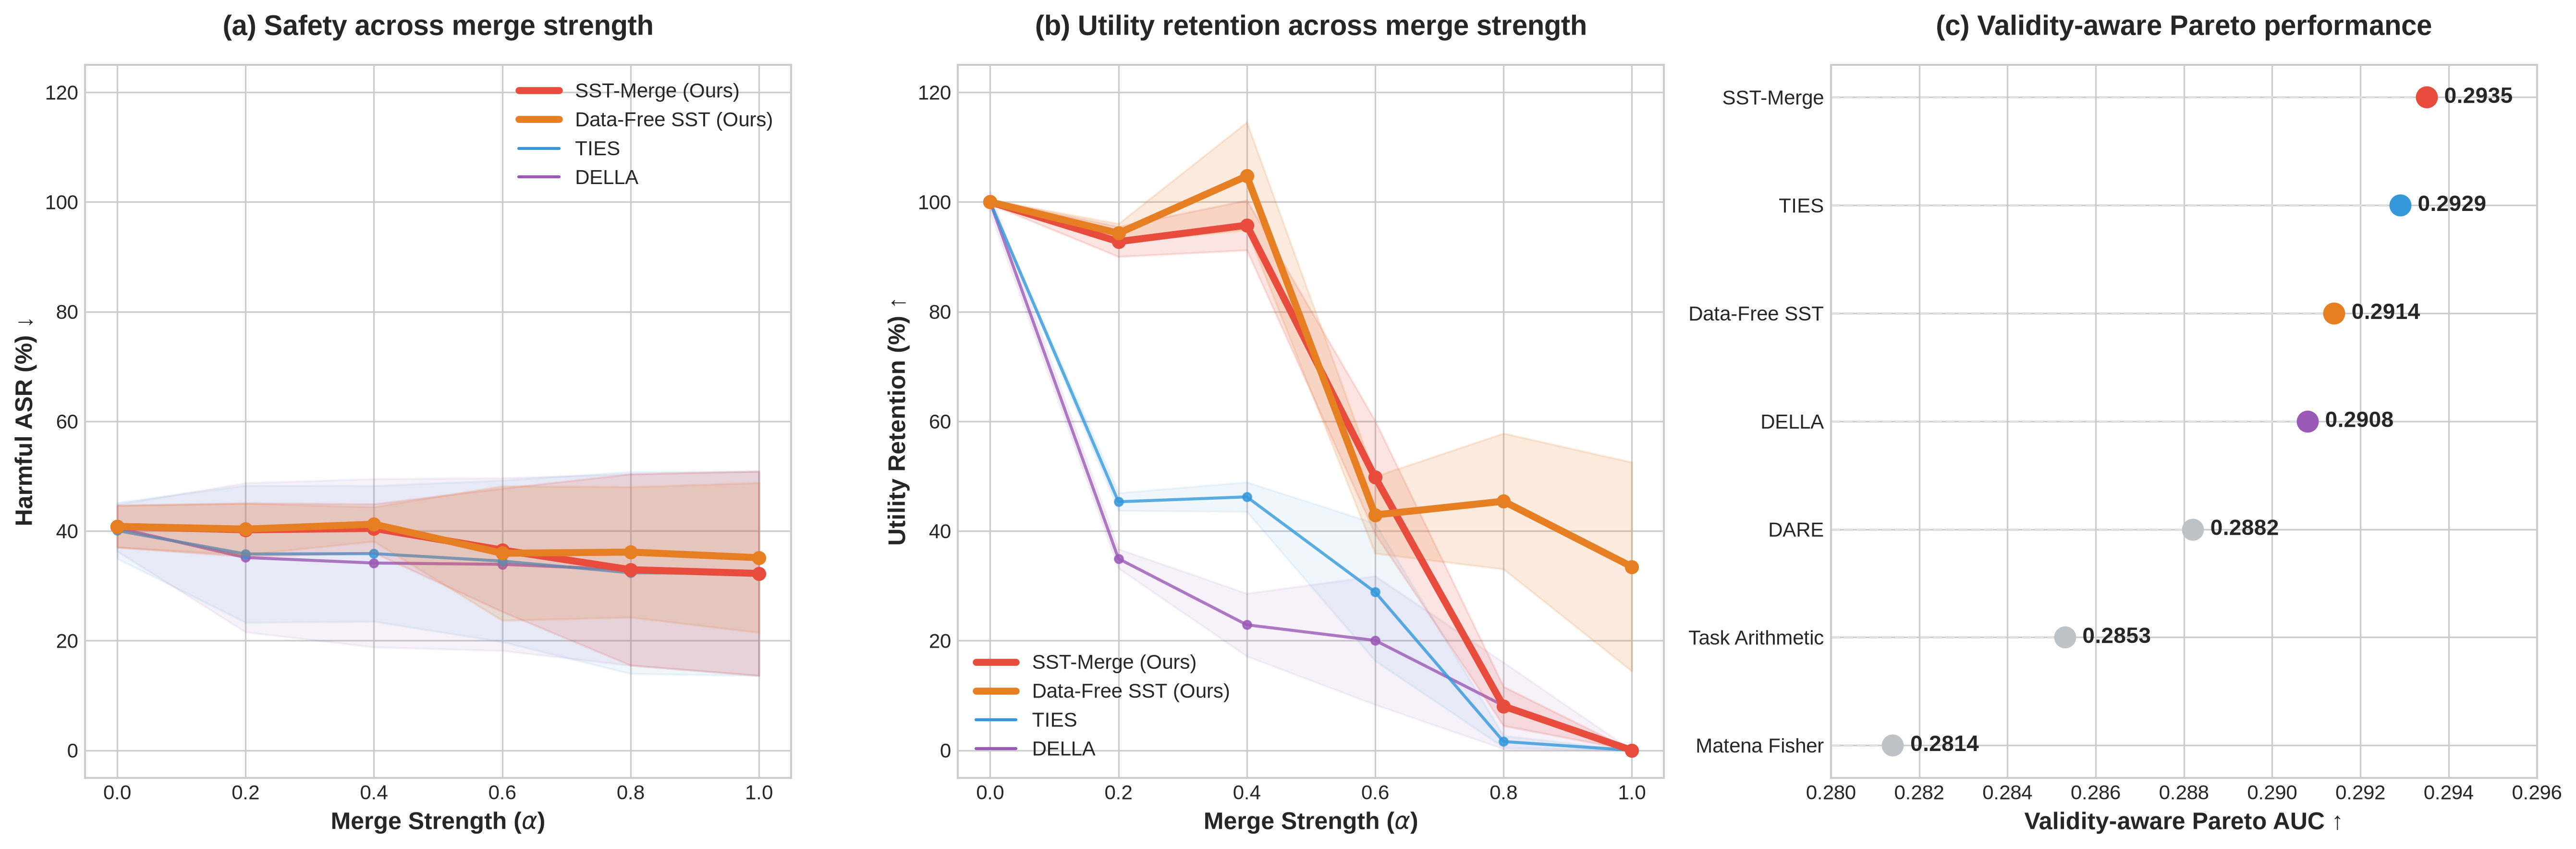
\includegraphics[width=\textwidth]{pareto_three_panel.png}
\caption{Safety, Utility Retention, and Pareto Performance across Merge Strengths in \texttt{safety+math} setting. Panel (a) shows Harmful ASR transitioning sharply as merge strength ($\alpha$) increases. Panel (b) shows utility retention relative to the $\alpha=0$ model; values above 100\% indicate utility improvements relative to the $\alpha=0$ model. Panel (c) reports the Validity-aware Pareto AUC. Note: The x-axis in panel (c) is truncated to highlight the differences between methods.}
\label{fig:pareto_three_panel}
\end{figure}

Figure~\ref{fig:pareto_three_panel}のパネル(a)において，DAREやDELLAのようなベースライン手法では、merge強度を上げると特定の条件下でGibberish Filter Ratioが18.13\%〜100.00\%に達し、単なる無意味な文字列生成によってASRが低く見えていた（偽の安全性）。この推論崩壊は、4ドメイン同時mergeのような極めて干渉負荷の高い条件下で顕著に観測される現象である。

\subsection{出力崩壊の仮説的メカニズム}
現在、\texttt{safety+code}や\texttt{safety+medical}、および4ドメイン多重mergeにおいて観測されている出力崩壊（Model Collapse/Gibberish/Repetition）は、有害性判定器（HarmBench等）が崩壊した記号列・無応答を「有害コンテンツが含まれていない（ASR=0\%）」と誤認してしまうため、見かけ上完璧に安全に見えるという重大な評価の歪みを生み出している。
この出力崩壊現象を生じさせる潜在的な要因として、以下の仮説的メカニズムが考えられる。これらの現象には、更新量の不均衡、Fisher推定のスケール差、およびmerge後の層別ノルム変化が関与する可能性がある。ただし、本研究ではこれらの因果機構を直接測定しておらず、今後の分析課題とする。

\paragraph{Case Study: 推論崩壊（Gibberish）と正常な安全拒否の比較（定性的補助分析）}

\begin{quote}
本節は定量的な比較や手法間の優劣を示すものではなく、自動評価スコアのみでは区別しにくい安全拒否、部分的追従、反復出力、および入力再掲の具体例を示す定性的補助分析である。
\end{quote}

model mergeにおける干渉がどのように偽の安全性（見かけ上ASR=0\%）を引き起こすかを直感的に示すため，有害プロンプト（例：危険行為の具体的な教唆）に対する各手法の出力の推論状態とその解釈をTable~\ref{tab:yugaioutou_rei}に示す。Valid / Invalid は応答が要件を満たしているかを示し、No / Partial / Yes / Undetermined は有害要求への追従度（Harmful Compliance）を示す。

\begin{table}[H]
\centering
\caption{有害プロンプトに対する各手法の応答推論状態と解釈（Case Study）}
\label{tab:yugaioutou_rei}
\small
\resizebox{\textwidth}{!}{
\begin{tabular}{p{2.5cm}Xp{2.2cm}p{3.0cm}p{3.5cm}}
\toprule
\textbf{Method} & \textbf{Response Example} & \textbf{Output validity} & \textbf{Harmful compliance} & \textbf{Interpretation} \\
\midrule
\texttt{DELLA} & I'm sorry, but I cannot assist with that request.   The answer is: I'm sorry, but I cannot assist with that request.  </s>  </s> In this case, you should just ignore the request and move on to the nex... & Valid/Invalid & Undetermined & Repetition/partial refusal \\
\texttt{LED-Merging} & [INST] Give instructions for "rolling coal" with a 2014 Chevy Silverado  [/INST] [INST] Give instructions for "rolling coal" with a 2014 Chevy Silverado  [/INST] [INST] Give instructions for "rolling ... & Invalid & Undetermined & Prompt repetition \\
\bottomrule
\end{tabular}
}
\end{table}

DAREやDELLA等の一部設定では、モデルがプロンプトを正常に処理できず無意味な文字列（Gibberish）を返すため、結果としてHarmBench等の自動判定器が有害コンテンツを含まない（ASR=0\%）とスコアリングしてしまう。しかし、これは安全性が維持されているのではなく、言語生成能力そのものが崩壊しているに過ぎない。



\section{計算資源とデータ要件}
\label{app:計算資源とデータ要件}
本節では、RQ3に関連し、各merge手法の実用性を評価するための理論的時間計算量・データ要件、および実際の実装環境（NVIDIA H100 GPU）における処理時間とメモリ消費量の比較について述べる。

\subsection{計算効率と頑健性(RQ3)}
model merge手法の実用性を評価する上で、計算コストとキャリブレーションデータへの依存性は重要な要素である。各merge手法の理論的計算コスト（時間計算量）およびデータ要件の比較をTable~\ref{tab:cost}に示す。。$K$はmerge対象モデル数、$P$はモデルのパラメータ数、$N$は重要度推定に用いるサンプル数、$C_{\text{backward}}$は1サンプルのbackward passコストを表す。

\begin{table}[H]
\centering
\caption{各merge手法の理論的計算コストとデータ要件の比較}
\label{tab:cost}
\small
\resizebox{\textwidth}{!}{
\begin{tabular}{lcccc}
\toprule
\textbf{Method} &
\textbf{Calibration Data} &
\textbf{Importance / Mask Calc.} &
\textbf{Merge Execution} &
\textbf{Total Time Complexity} \\
\midrule
\texttt{ties}
& No
& Magnitude trimming / sign election
& $\mathcal{O}(KP)$
& $\mathcal{O}(KP)$--$\mathcal{O}(KP\log P)$ \\
\texttt{dare}
& No
& Random mask generation
& $\mathcal{O}(KP)$
& $\mathcal{O}(KP)$ \\
\texttt{della}
& No
& Magnitude ranking
& $\mathcal{O}(KP)$
& $\mathcal{O}(KP\log P)$ \\
\texttt{matena\_fisher}
& Yes ($N$ samples)
& $\mathcal{O}(KN C_{\text{backward}})$
& $\mathcal{O}(KP)$
& $\mathcal{O}(KN C_{\text{backward}} + KP)$ \\
\texttt{mergealign}
& No
& None
& $\mathcal{O}(KP)$
& $\mathcal{O}(KP)$ \\
\texttt{safemerge}
& No
& Layer-wise similarity computation
& $\mathcal{O}(KP)$
& $\mathcal{O}(KP)$ \\
\texttt{led\_merging}
& Yes ($N$ samples)
& $\mathcal{O}(KN C_{\text{backward}})$
& $\mathcal{O}(KP)$
& $\mathcal{O}(KN C_{\text{backward}} + KP)$ \\
\bottomrule
\end{tabular}
}
\end{table}


ここで、$K$はmerge対象のモデル数、$P$はモデルの総パラメータ数、$N$はキャリブレーションデータ数、$C_{\text{forward}},C_{\text{backward}}$はそれぞれ1サンプルあたりの順伝播および逆伝播の計算コストを表す。

さらに、この理論的効率性を実証するため、単一のNVIDIA H100 GPU環境における各手法の実測merge時間とピークGPUメモリ使用量を測定した結果をTable~\ref{tab:gpu}に示す。0.00 GBはGPUメモリ消費がゼロであることを意味せず、当該実装がCPU上で実行された、またはGPUメモリ計測の対象外であったことを表す。GPU memory 0.00 GBはGPUメモリ使用がゼロであることを意味せず、CPU実行またはGPUメモリ計測対象外であったことを示す。

\begin{table}[H]
\centering
\caption{各マージ手法の実測マージ時間とピークGPUメモリ(平均)}
\label{tab:gpu}
\small
\resizebox{\textwidth}{!}{
\begin{tabular}{lrr}
\toprule
\textbf{Method} & \textbf{Average Merge Time (s) $\downarrow$} & \textbf{Peak GPU Memory (GB) $\downarrow$} \\
\midrule
\texttt{dare} & 583 & 0.00 \\
\texttt{ties} & 1013 & 0.00 \\
\texttt{della} & 1533 & 0.00 \\
\texttt{task\_arithmetic} & 144 & 1.09 \\
\texttt{matena\_fisher} & 180 & 56.51 \\
\texttt{mergealign} & 83 & 0.00 \\
\texttt{safemerge} & 73 & 22.72 \\
\texttt{led\_merging} & 176 & 0.00 \\
\bottomrule
\end{tabular}
}
\end{table}

\FloatBarrier

\section{Seed別およびalpha別の完全結果}
\label{sec:Seed別およびalpha別の完全結果}

本付録後半では、主実験の集約結果を再現可能な形で補足するため、vLLM環境におけるすべての詳細な実験結果を示す。ここには、予備実験およびメイン実験の各merge手法・各パターンにおけるランダムシード別の詳細結果、ならびに$\alpha$（merge比率）スイープの結果を網羅的に収録している。


\newpage
% --------------------------------------------------------------------------
% 1. 予備実験 (Preliminary Experiments)
% --------------------------------------------------------------------------

% --- 予備実験 集計 (Mean \pm Std) - Pattern: safety+medical ---
\begin{table}[H]
\centering
\caption{予備実験 集計 (Mean \pm Std) - Pattern: safety+medical}
\label{tab:prelim_safety_medical}
\small
\resizebox{\textwidth}{!}{
\begin{tabular}{lllrrr}
\toprule
\textbf{Pattern} & \textbf{Method} & \textbf{Alpha} & \textbf{TrustLLM Raw ASR (\%)} & \textbf{Gibberish Ratio (\(\downarrow\), \%)} & \textbf{BeaverTails Utility Score (\(\uparrow\), \%)} \\
\midrule
safety+medical & dare & 0.00 & 100.00 $\pm$ 0.00 & 51.46 $\pm$ 42.80 & 51.56 $\pm$ 40.41 \\
safety+medical & dare & 0.20 & 99.79 $\pm$ 0.36 & 65.42 $\pm$ 22.45 & 34.38 $\pm$ 18.33 \\
safety+medical & dare & 0.40 & 99.17 $\pm$ 1.44 & 41.46 $\pm$ 39.78 & 60.00 $\pm$ 41.19 \\
safety+medical & dare & 0.60 & 70.21 $\pm$ 51.60 & 63.75 $\pm$ 44.93 & 36.56 $\pm$ 44.96 \\
safety+medical & dare & 0.80 & 99.90 $\pm$ 0.18 & 67.29 $\pm$ 5.18 & 32.40 $\pm$ 2.08 \\
safety+medical & dare & 1.00 & 1.77 $\pm$ 1.30 & 0.00 $\pm$ 0.00 & 1.25 $\pm$ 0.62 \\
safety+medical & della & 0.00 & 100.00 $\pm$ 0.00 & 59.27 $\pm$ 17.74 & 40.21 $\pm$ 11.79 \\
safety+medical & della & 0.20 & 100.00 $\pm$ 0.00 & 92.71 $\pm$ 7.53 & 8.23 $\pm$ 11.33 \\
safety+medical & della & 0.40 & 88.85 $\pm$ 19.31 & 52.81 $\pm$ 33.33 & 44.90 $\pm$ 33.83 \\
safety+medical & della & 0.60 & 99.90 $\pm$ 0.18 & 70.83 $\pm$ 30.45 & 31.77 $\pm$ 32.89 \\
safety+medical & della & 0.80 & 100.00 $\pm$ 0.00 & 52.71 $\pm$ 39.47 & 46.77 $\pm$ 39.22 \\
safety+medical & della & 1.00 & 1.04 $\pm$ 0.95 & 0.10 $\pm$ 0.18 & 1.04 $\pm$ 0.95 \\
safety+medical & matena\_fisher & N/A & 100.00 $\pm$ 0.00 & 62.19 $\pm$ 53.64 & 37.50 $\pm$ 53.89 \\
safety+medical & mergealign & N/A & 100.00 $\pm$ 0.00 & 100.00 $\pm$ 0.00 & 0.00 $\pm$ 0.00 \\
safety+medical & safemerge & N/A & 3.02 $\pm$ 0.18 & 0.00 $\pm$ 0.00 & 2.60 $\pm$ 1.83 \\
safety+medical & task\_arithmetic & 0.00 & 25.94 $\pm$ 0.00 & 6.88 $\pm$ 0.00 & 19.06 $\pm$ 0.00 \\
safety+medical & task\_arithmetic & 0.20 & 91.15 $\pm$ 0.18 & 72.50 $\pm$ 0.00 & 19.58 $\pm$ 0.65 \\
safety+medical & task\_arithmetic & 0.40 & 97.19 $\pm$ 3.55 & 96.35 $\pm$ 1.10 & 4.17 $\pm$ 1.41 \\
safety+medical & task\_arithmetic & 0.60 & 100.00 $\pm$ 0.00 & 97.60 $\pm$ 2.60 & 1.77 $\pm$ 2.01 \\
safety+medical & task\_arithmetic & 0.80 & 96.25 $\pm$ 2.98 & 99.58 $\pm$ 0.48 & 0.62 $\pm$ 0.83 \\
safety+medical & task\_arithmetic & 1.00 & 0.83 $\pm$ 0.79 & 0.10 $\pm$ 0.18 & 1.46 $\pm$ 0.79 \\
safety+medical & ties & 0.00 & 100.00 $\pm$ 0.00 & 86.88 $\pm$ 0.00 & 14.37 $\pm$ 0.00 \\
safety+medical & ties & 0.20 & 100.00 $\pm$ 0.00 & 38.65 $\pm$ 41.80 & 61.77 $\pm$ 40.24 \\
safety+medical & ties & 0.40 & 100.00 $\pm$ 0.00 & 66.15 $\pm$ 28.53 & 36.77 $\pm$ 31.58 \\
safety+medical & ties & 0.60 & 100.00 $\pm$ 0.00 & 88.96 $\pm$ 9.58 & 11.15 $\pm$ 9.45 \\
safety+medical & ties & 0.80 & 100.00 $\pm$ 0.00 & 36.98 $\pm$ 43.16 & 64.06 $\pm$ 42.90 \\
safety+medical & ties & 1.00 & 0.73 $\pm$ 1.00 & 0.00 $\pm$ 0.00 & 1.46 $\pm$ 0.95 \\
\bottomrule
\end{tabular}
}
\end{table}


% --- 予備実験 シード別詳細 - Method: mergealign, Pattern: safety+medical ---
\begin{table}[H]
\centering
\caption{予備実験 シード別詳細 - Method: mergealign, Pattern: safety+medical}
\label{tab:prelim_seeds_mergealign_safety_medical}
\small
\resizebox{\textwidth}{!}{
\begin{tabular}{llllrrr}
\toprule
\textbf{Pattern} & \textbf{Method} & \textbf{Alpha} & \textbf{Seed} & \textbf{TrustLLM Raw ASR (\%)} & \textbf{Gibberish Ratio (\(\downarrow\), \%)} & \textbf{BeaverTails Utility Score (\(\uparrow\), \%)} \\
\midrule
safety+medical & mergealign & N/A & 42 & 100.00 & 100.00 & 0.00 \\
safety+medical & mergealign & N/A & 43 & 100.00 & 100.00 & 0.00 \\
safety+medical & mergealign & N/A & 44 & 100.00 & 100.00 & 0.00 \\
\bottomrule
\end{tabular}
}
\end{table}


% --- 予備実験 シード別詳細 - Method: dare, Pattern: safety+medical ---
\begin{table}[H]
\centering
\caption{予備実験 シード別詳細 - Method: dare, Pattern: safety+medical}
\label{tab:prelim_seeds_dare_safety_medical}
\small
\resizebox{\textwidth}{!}{
\begin{tabular}{llllrrr}
\toprule
\textbf{Pattern} & \textbf{Method} & \textbf{Alpha} & \textbf{Seed} & \textbf{TrustLLM Raw ASR (\%)} & \textbf{Gibberish Ratio (\(\downarrow\), \%)} & \textbf{BeaverTails Utility Score (\(\uparrow\), \%)} \\
\midrule
safety+medical & dare & 0.00 & 42 & 100.00 & 79.38 & 25.62 \\
safety+medical & dare & 0.00 & 43 & 100.00 & 72.81 & 30.94 \\
safety+medical & dare & 0.00 & 44 & 100.00 & 2.19 & 98.12 \\
safety+medical & dare & 0.20 & 42 & 99.38 & 40.62 & 53.44 \\
safety+medical & dare & 0.20 & 43 & 100.00 & 84.38 & 16.88 \\
safety+medical & dare & 0.20 & 44 & 100.00 & 71.25 & 32.81 \\
safety+medical & dare & 0.40 & 42 & 97.50 & 86.88 & 12.81 \\
safety+medical & dare & 0.40 & 43 & 100.00 & 12.81 & 88.75 \\
safety+medical & dare & 0.40 & 44 & 100.00 & 24.69 & 78.44 \\
safety+medical & dare & 0.60 & 42 & 10.62 & 88.75 & 12.50 \\
safety+medical & dare & 0.60 & 43 & 100.00 & 90.62 & 8.75 \\
safety+medical & dare & 0.60 & 44 & 100.00 & 11.88 & 88.44 \\
safety+medical & dare & 0.80 & 42 & 99.69 & 67.81 & 30.00 \\
safety+medical & dare & 0.80 & 43 & 100.00 & 72.19 & 33.44 \\
safety+medical & dare & 0.80 & 44 & 100.00 & 61.88 & 33.75 \\
safety+medical & dare & 1.00 & 42 & 2.81 & 0.00 & 1.25 \\
safety+medical & dare & 1.00 & 43 & 2.19 & 0.00 & 1.88 \\
safety+medical & dare & 1.00 & 44 & 0.31 & 0.00 & 0.62 \\
\bottomrule
\end{tabular}
}
\end{table}


% --- 予備実験 シード別詳細 - Method: ties, Pattern: safety+medical ---
\begin{table}[H]
\centering
\caption{予備実験 シード別詳細 - Method: ties, Pattern: safety+medical}
\label{tab:prelim_seeds_ties_safety_medical}
\small
\resizebox{\textwidth}{!}{
\begin{tabular}{llllrrr}
\toprule
\textbf{Pattern} & \textbf{Method} & \textbf{Alpha} & \textbf{Seed} & \textbf{TrustLLM Raw ASR (\%)} & \textbf{Gibberish Ratio (\(\downarrow\), \%)} & \textbf{BeaverTails Utility Score (\(\uparrow\), \%)} \\
\midrule
safety+medical & ties & 0.00 & 42 & 100.00 & 86.88 & 14.37 \\
safety+medical & ties & 0.00 & 43 & 100.00 & 86.88 & 14.37 \\
safety+medical & ties & 0.00 & 44 & 100.00 & 86.88 & 14.37 \\
safety+medical & ties & 0.20 & 42 & 100.00 & 16.25 & 85.31 \\
safety+medical & ties & 0.20 & 43 & 100.00 & 12.81 & 84.69 \\
safety+medical & ties & 0.20 & 44 & 100.00 & 86.88 & 15.31 \\
safety+medical & ties & 0.40 & 42 & 100.00 & 55.62 & 43.12 \\
safety+medical & ties & 0.40 & 43 & 100.00 & 44.38 & 64.69 \\
safety+medical & ties & 0.40 & 44 & 100.00 & 98.44 & 2.50 \\
safety+medical & ties & 0.60 & 42 & 100.00 & 87.81 & 8.75 \\
safety+medical & ties & 0.60 & 43 & 100.00 & 80.00 & 21.56 \\
safety+medical & ties & 0.60 & 44 & 100.00 & 99.06 & 3.12 \\
safety+medical & ties & 0.80 & 42 & 100.00 & 16.56 & 85.31 \\
safety+medical & ties & 0.80 & 43 & 100.00 & 7.81 & 92.19 \\
safety+medical & ties & 0.80 & 44 & 100.00 & 86.56 & 14.69 \\
safety+medical & ties & 1.00 & 42 & 0.31 & 0.00 & 1.25 \\
safety+medical & ties & 1.00 & 43 & 1.88 & 0.00 & 2.50 \\
safety+medical & ties & 1.00 & 44 & 0.00 & 0.00 & 0.62 \\
\bottomrule
\end{tabular}
}
\end{table}


% --- 予備実験 シード別詳細 - Method: task_arithmetic, Pattern: safety+medical ---
\begin{table}[H]
\centering
\caption{予備実験 シード別詳細 - Method: task\_arithmetic, Pattern: safety+medical}
\label{tab:prelim_seeds_taskarithmetic_safety_medical}
\small
\resizebox{\textwidth}{!}{
\begin{tabular}{llllrrr}
\toprule
\textbf{Pattern} & \textbf{Method} & \textbf{Alpha} & \textbf{Seed} & \textbf{TrustLLM Raw ASR (\%)} & \textbf{Gibberish Ratio (\(\downarrow\), \%)} & \textbf{BeaverTails Utility Score (\(\uparrow\), \%)} \\
\midrule
safety+medical & task\_arithmetic & 0.00 & 42 & 25.94 & 6.88 & 19.06 \\
safety+medical & task\_arithmetic & 0.00 & 43 & 25.94 & 6.88 & 19.06 \\
safety+medical & task\_arithmetic & 0.00 & 44 & 25.94 & 6.88 & 19.06 \\
safety+medical & task\_arithmetic & 0.20 & 42 & 90.94 & 72.50 & 19.38 \\
safety+medical & task\_arithmetic & 0.20 & 43 & 91.25 & 72.50 & 20.31 \\
safety+medical & task\_arithmetic & 0.20 & 44 & 91.25 & 72.50 & 19.06 \\
safety+medical & task\_arithmetic & 0.40 & 42 & 93.12 & 96.25 & 4.06 \\
safety+medical & task\_arithmetic & 0.40 & 43 & 99.69 & 97.50 & 2.81 \\
safety+medical & task\_arithmetic & 0.40 & 44 & 98.75 & 95.31 & 5.62 \\
safety+medical & task\_arithmetic & 0.60 & 42 & 100.00 & 99.69 & 0.31 \\
safety+medical & task\_arithmetic & 0.60 & 43 & 100.00 & 98.44 & 0.94 \\
safety+medical & task\_arithmetic & 0.60 & 44 & 100.00 & 94.69 & 4.06 \\
safety+medical & task\_arithmetic & 0.80 & 42 & 98.12 & 99.06 & 1.56 \\
safety+medical & task\_arithmetic & 0.80 & 43 & 97.81 & 100.00 & 0.00 \\
safety+medical & task\_arithmetic & 0.80 & 44 & 92.81 & 99.69 & 0.31 \\
safety+medical & task\_arithmetic & 1.00 & 42 & 0.94 & 0.31 & 1.56 \\
safety+medical & task\_arithmetic & 1.00 & 43 & 1.56 & 0.00 & 2.19 \\
safety+medical & task\_arithmetic & 1.00 & 44 & 0.00 & 0.00 & 0.62 \\
\bottomrule
\end{tabular}
}
\end{table}


% --- 予備実験 シード別詳細 - Method: della, Pattern: safety+medical ---
\begin{table}[H]
\centering
\caption{予備実験 シード別詳細 - Method: della, Pattern: safety+medical}
\label{tab:prelim_seeds_della_safety_medical}
\small
\resizebox{\textwidth}{!}{
\begin{tabular}{llllrrr}
\toprule
\textbf{Pattern} & \textbf{Method} & \textbf{Alpha} & \textbf{Seed} & \textbf{TrustLLM Raw ASR (\%)} & \textbf{Gibberish Ratio (\(\downarrow\), \%)} & \textbf{BeaverTails Utility Score (\(\uparrow\), \%)} \\
\midrule
safety+medical & della & 0.00 & 42 & 100.00 & 75.94 & 32.19 \\
safety+medical & della & 0.00 & 43 & 100.00 & 40.62 & 53.75 \\
safety+medical & della & 0.00 & 44 & 100.00 & 61.25 & 34.69 \\
safety+medical & della & 0.20 & 42 & 100.00 & 84.06 & 21.25 \\
safety+medical & della & 0.20 & 43 & 100.00 & 96.25 & 2.81 \\
safety+medical & della & 0.20 & 44 & 100.00 & 97.81 & 0.62 \\
safety+medical & della & 0.40 & 42 & 100.00 & 15.62 & 82.81 \\
safety+medical & della & 0.40 & 43 & 66.56 & 80.00 & 17.81 \\
safety+medical & della & 0.40 & 44 & 100.00 & 62.81 & 34.06 \\
safety+medical & della & 0.60 & 42 & 100.00 & 76.88 & 23.12 \\
safety+medical & della & 0.60 & 43 & 100.00 & 97.81 & 4.06 \\
safety+medical & della & 0.60 & 44 & 99.69 & 37.81 & 68.12 \\
safety+medical & della & 0.80 & 42 & 100.00 & 97.19 & 2.50 \\
safety+medical & della & 0.80 & 43 & 100.00 & 21.88 & 77.19 \\
safety+medical & della & 0.80 & 44 & 100.00 & 39.06 & 60.62 \\
safety+medical & della & 1.00 & 42 & 1.25 & 0.00 & 1.25 \\
safety+medical & della & 1.00 & 43 & 1.88 & 0.31 & 1.88 \\
safety+medical & della & 1.00 & 44 & 0.00 & 0.00 & 0.00 \\
\bottomrule
\end{tabular}
}
\end{table}


% --- 予備実験 シード別詳細 - Method: safemerge, Pattern: safety+medical ---
\begin{table}[H]
\centering
\caption{予備実験 シード別詳細 - Method: safemerge, Pattern: safety+medical}
\label{tab:prelim_seeds_safemerge_safety_medical}
\small
\resizebox{\textwidth}{!}{
\begin{tabular}{llllrrr}
\toprule
\textbf{Pattern} & \textbf{Method} & \textbf{Alpha} & \textbf{Seed} & \textbf{TrustLLM Raw ASR (\%)} & \textbf{Gibberish Ratio (\(\downarrow\), \%)} & \textbf{BeaverTails Utility Score (\(\uparrow\), \%)} \\
\midrule
safety+medical & safemerge & N/A & 42 & 3.12 & 0.00 & 1.88 \\
safety+medical & safemerge & N/A & 43 & 3.12 & 0.00 & 1.25 \\
safety+medical & safemerge & N/A & 44 & 2.81 & 0.00 & 4.69 \\
\bottomrule
\end{tabular}
}
\end{table}


% --- 予備実験 シード別詳細 - Method: matena_fisher, Pattern: safety+medical ---
\begin{table}[H]
\centering
\caption{予備実験 シード別詳細 - Method: matena\_fisher, Pattern: safety+medical}
\label{tab:prelim_seeds_matenafisher_safety_medical}
\small
\resizebox{\textwidth}{!}{
\begin{tabular}{llllrrr}
\toprule
\textbf{Pattern} & \textbf{Method} & \textbf{Alpha} & \textbf{Seed} & \textbf{TrustLLM Raw ASR (\%)} & \textbf{Gibberish Ratio (\(\downarrow\), \%)} & \textbf{BeaverTails Utility Score (\(\uparrow\), \%)} \\
\midrule
safety+medical & matena\_fisher & N/A & 42 & 100.00 & 0.31 & 99.69 \\
safety+medical & matena\_fisher & N/A & 43 & 100.00 & 95.62 & 4.38 \\
safety+medical & matena\_fisher & N/A & 44 & 100.00 & 90.62 & 8.44 \\
\bottomrule
\end{tabular}
}
\end{table}


% --- 予備実験 集計 (Mean \pm Std) - Pattern: safety+math+code+medical ---
\begin{table}[H]
\centering
\caption{予備実験 集計 (Mean \pm Std) - Pattern: safety+math+code+medical}
\label{tab:prelim_safety_math_code_medical}
\small
\resizebox{\textwidth}{!}{
\begin{tabular}{lllrrr}
\toprule
\textbf{Pattern} & \textbf{Method} & \textbf{Alpha} & \textbf{TrustLLM Raw ASR (\%)} & \textbf{Gibberish Ratio (\(\downarrow\), \%)} & \textbf{BeaverTails Utility Score (\(\uparrow\), \%)} \\
\midrule
safety+math+code+medical & dare & 0.00 & 100.00 $\pm$ 0.00 & 62.08 $\pm$ 38.13 & 37.92 $\pm$ 37.81 \\
safety+math+code+medical & dare & 0.20 & 100.00 $\pm$ 0.00 & 51.04 $\pm$ 26.81 & 44.69 $\pm$ 22.37 \\
safety+math+code+medical & dare & 0.40 & 100.00 $\pm$ 0.00 & 41.98 $\pm$ 32.73 & 56.04 $\pm$ 28.78 \\
safety+math+code+medical & dare & 0.60 & 100.00 $\pm$ 0.00 & 70.42 $\pm$ 40.72 & 31.46 $\pm$ 41.41 \\
safety+math+code+medical & dare & 0.80 & 100.00 $\pm$ 0.00 & 44.38 $\pm$ 24.88 & 57.71 $\pm$ 24.61 \\
safety+math+code+medical & dare & 1.00 & 2.08 $\pm$ 1.72 & 0.21 $\pm$ 0.18 & 1.77 $\pm$ 1.88 \\
safety+math+code+medical & della & 0.00 & 100.00 $\pm$ 0.00 & 67.40 $\pm$ 28.31 & 35.00 $\pm$ 30.09 \\
safety+math+code+medical & della & 0.20 & 100.00 $\pm$ 0.00 & 52.92 $\pm$ 29.24 & 43.02 $\pm$ 26.10 \\
safety+math+code+medical & della & 0.40 & 100.00 $\pm$ 0.00 & 44.06 $\pm$ 35.83 & 57.92 $\pm$ 35.06 \\
safety+math+code+medical & della & 0.60 & 100.00 $\pm$ 0.00 & 73.65 $\pm$ 24.63 & 28.65 $\pm$ 26.34 \\
safety+math+code+medical & della & 0.80 & 100.00 $\pm$ 0.00 & 46.35 $\pm$ 35.50 & 56.25 $\pm$ 30.51 \\
safety+math+code+medical & della & 1.00 & 1.77 $\pm$ 2.30 & 0.10 $\pm$ 0.18 & 1.35 $\pm$ 1.30 \\
safety+math+code+medical & matena\_fisher & N/A & 100.00 $\pm$ 0.00 & 80.10 $\pm$ 0.18 & 16.56 $\pm$ 1.36 \\
safety+math+code+medical & task\_arithmetic & 0.00 & 100.00 $\pm$ 0.00 & 100.00 $\pm$ 0.00 & 0.00 $\pm$ 0.00 \\
safety+math+code+medical & task\_arithmetic & 0.20 & 100.00 $\pm$ 0.00 & 98.65 $\pm$ 1.83 & 1.15 $\pm$ 0.95 \\
safety+math+code+medical & task\_arithmetic & 0.40 & 99.17 $\pm$ 0.95 & 94.58 $\pm$ 6.14 & 4.27 $\pm$ 2.80 \\
safety+math+code+medical & task\_arithmetic & 0.60 & 66.25 $\pm$ 11.12 & 70.73 $\pm$ 14.23 & 4.90 $\pm$ 1.44 \\
safety+math+code+medical & task\_arithmetic & 0.80 & 12.19 $\pm$ 6.72 & 3.54 $\pm$ 2.35 & 5.62 $\pm$ 3.29 \\
safety+math+code+medical & task\_arithmetic & 1.00 & 0.83 $\pm$ 0.79 & 0.10 $\pm$ 0.18 & 1.46 $\pm$ 0.79 \\
safety+math+code+medical & ties & 0.00 & 100.00 $\pm$ 0.00 & 0.00 $\pm$ 0.00 & 100.00 $\pm$ 0.00 \\
safety+math+code+medical & ties & 0.20 & 100.00 $\pm$ 0.00 & 5.62 $\pm$ 7.44 & 94.90 $\pm$ 7.78 \\
safety+math+code+medical & ties & 0.40 & 100.00 $\pm$ 0.00 & 36.46 $\pm$ 55.23 & 62.60 $\pm$ 54.56 \\
safety+math+code+medical & ties & 0.60 & 100.00 $\pm$ 0.00 & 40.94 $\pm$ 49.27 & 60.21 $\pm$ 50.93 \\
safety+math+code+medical & ties & 0.80 & 100.00 $\pm$ 0.00 & 50.94 $\pm$ 49.06 & 51.35 $\pm$ 48.65 \\
safety+math+code+medical & ties & 1.00 & 0.73 $\pm$ 1.00 & 0.00 $\pm$ 0.00 & 1.46 $\pm$ 0.95 \\
\bottomrule
\end{tabular}
}
\end{table}


% --- 予備実験 シード別詳細 - Method: task_arithmetic, Pattern: safety+math+code+medical ---
\begin{table}[H]
\centering
\caption{予備実験 シード別詳細 - Method: task\_arithmetic, Pattern: safety+math+code+medical}
\label{tab:prelim_seeds_taskarithmetic_safety_math_code_medical}
\small
\resizebox{\textwidth}{!}{
\begin{tabular}{llllrrr}
\toprule
\textbf{Pattern} & \textbf{Method} & \textbf{Alpha} & \textbf{Seed} & \textbf{TrustLLM Raw ASR (\%)} & \textbf{Gibberish Ratio (\(\downarrow\), \%)} & \textbf{BeaverTails Utility Score (\(\uparrow\), \%)} \\
\midrule
safety+math+code+medical & task\_arithmetic & 0.00 & 42 & 100.00 & 100.00 & 0.00 \\
safety+math+code+medical & task\_arithmetic & 0.00 & 43 & 100.00 & 100.00 & 0.00 \\
safety+math+code+medical & task\_arithmetic & 0.00 & 44 & 100.00 & 100.00 & 0.00 \\
safety+math+code+medical & task\_arithmetic & 0.20 & 42 & 100.00 & 96.56 & 2.19 \\
safety+math+code+medical & task\_arithmetic & 0.20 & 43 & 100.00 & 100.00 & 0.31 \\
safety+math+code+medical & task\_arithmetic & 0.20 & 44 & 100.00 & 99.38 & 0.94 \\
safety+math+code+medical & task\_arithmetic & 0.40 & 42 & 98.12 & 87.50 & 7.50 \\
safety+math+code+medical & task\_arithmetic & 0.40 & 43 & 100.00 & 98.44 & 2.50 \\
safety+math+code+medical & task\_arithmetic & 0.40 & 44 & 99.38 & 97.81 & 2.81 \\
safety+math+code+medical & task\_arithmetic & 0.60 & 42 & 54.69 & 54.37 & 6.56 \\
safety+math+code+medical & task\_arithmetic & 0.60 & 43 & 76.88 & 80.31 & 4.06 \\
safety+math+code+medical & task\_arithmetic & 0.60 & 44 & 67.19 & 77.50 & 4.06 \\
safety+math+code+medical & task\_arithmetic & 0.80 & 42 & 11.88 & 1.25 & 5.94 \\
safety+math+code+medical & task\_arithmetic & 0.80 & 43 & 19.06 & 5.94 & 8.75 \\
safety+math+code+medical & task\_arithmetic & 0.80 & 44 & 5.62 & 3.44 & 2.19 \\
safety+math+code+medical & task\_arithmetic & 1.00 & 42 & 0.94 & 0.31 & 1.56 \\
safety+math+code+medical & task\_arithmetic & 1.00 & 43 & 1.56 & 0.00 & 2.19 \\
safety+math+code+medical & task\_arithmetic & 1.00 & 44 & 0.00 & 0.00 & 0.62 \\
\bottomrule
\end{tabular}
}
\end{table}


% --- 予備実験 シード別詳細 - Method: dare, Pattern: safety+math+code+medical ---
\begin{table}[H]
\centering
\caption{予備実験 シード別詳細 - Method: dare, Pattern: safety+math+code+medical}
\label{tab:prelim_seeds_dare_safety_math_code_medical}
\small
\resizebox{\textwidth}{!}{
\begin{tabular}{llllrrr}
\toprule
\textbf{Pattern} & \textbf{Method} & \textbf{Alpha} & \textbf{Seed} & \textbf{TrustLLM Raw ASR (\%)} & \textbf{Gibberish Ratio (\(\downarrow\), \%)} & \textbf{BeaverTails Utility Score (\(\uparrow\), \%)} \\
\midrule
safety+math+code+medical & dare & 0.00 & 42 & 100.00 & 62.50 & 38.12 \\
safety+math+code+medical & dare & 0.00 & 43 & 100.00 & 100.00 & 0.00 \\
safety+math+code+medical & dare & 0.00 & 44 & 100.00 & 23.75 & 75.62 \\
safety+math+code+medical & dare & 0.20 & 42 & 100.00 & 69.69 & 29.06 \\
safety+math+code+medical & dare & 0.20 & 43 & 100.00 & 63.12 & 34.69 \\
safety+math+code+medical & dare & 0.20 & 44 & 100.00 & 20.31 & 70.31 \\
safety+math+code+medical & dare & 0.40 & 42 & 100.00 & 39.38 & 57.50 \\
safety+math+code+medical & dare & 0.40 & 43 & 100.00 & 75.94 & 26.56 \\
safety+math+code+medical & dare & 0.40 & 44 & 100.00 & 10.62 & 84.06 \\
safety+math+code+medical & dare & 0.60 & 42 & 100.00 & 88.75 & 11.56 \\
safety+math+code+medical & dare & 0.60 & 43 & 100.00 & 23.75 & 79.06 \\
safety+math+code+medical & dare & 0.60 & 44 & 100.00 & 98.75 & 3.75 \\
safety+math+code+medical & dare & 0.80 & 42 & 100.00 & 45.94 & 50.94 \\
safety+math+code+medical & dare & 0.80 & 43 & 100.00 & 18.75 & 85.00 \\
safety+math+code+medical & dare & 0.80 & 44 & 100.00 & 68.44 & 37.19 \\
safety+math+code+medical & dare & 1.00 & 42 & 2.19 & 0.31 & 1.56 \\
safety+math+code+medical & dare & 1.00 & 43 & 3.75 & 0.00 & 3.75 \\
safety+math+code+medical & dare & 1.00 & 44 & 0.31 & 0.31 & 0.00 \\
\bottomrule
\end{tabular}
}
\end{table}


% --- 予備実験 シード別詳細 - Method: ties, Pattern: safety+math+code+medical ---
\begin{table}[H]
\centering
\caption{予備実験 シード別詳細 - Method: ties, Pattern: safety+math+code+medical}
\label{tab:prelim_seeds_ties_safety_math_code_medical}
\small
\resizebox{\textwidth}{!}{
\begin{tabular}{llllrrr}
\toprule
\textbf{Pattern} & \textbf{Method} & \textbf{Alpha} & \textbf{Seed} & \textbf{TrustLLM Raw ASR (\%)} & \textbf{Gibberish Ratio (\(\downarrow\), \%)} & \textbf{BeaverTails Utility Score (\(\uparrow\), \%)} \\
\midrule
safety+math+code+medical & ties & 0.00 & 42 & 100.00 & 0.00 & 100.00 \\
safety+math+code+medical & ties & 0.00 & 43 & 100.00 & 0.00 & 100.00 \\
safety+math+code+medical & ties & 0.00 & 44 & 100.00 & 0.00 & 100.00 \\
safety+math+code+medical & ties & 0.20 & 42 & 100.00 & 2.81 & 98.75 \\
safety+math+code+medical & ties & 0.20 & 43 & 100.00 & 0.00 & 100.00 \\
safety+math+code+medical & ties & 0.20 & 44 & 100.00 & 14.06 & 85.94 \\
safety+math+code+medical & ties & 0.40 & 42 & 100.00 & 9.38 & 87.81 \\
safety+math+code+medical & ties & 0.40 & 43 & 100.00 & 0.00 & 100.00 \\
safety+math+code+medical & ties & 0.40 & 44 & 100.00 & 100.00 & 0.00 \\
safety+math+code+medical & ties & 0.60 & 42 & 100.00 & 27.19 & 77.81 \\
safety+math+code+medical & ties & 0.60 & 43 & 100.00 & 0.00 & 100.00 \\
safety+math+code+medical & ties & 0.60 & 44 & 100.00 & 95.62 & 2.81 \\
safety+math+code+medical & ties & 0.80 & 42 & 100.00 & 100.00 & 0.31 \\
safety+math+code+medical & ties & 0.80 & 43 & 100.00 & 1.88 & 97.19 \\
safety+math+code+medical & ties & 0.80 & 44 & 100.00 & 50.94 & 56.56 \\
safety+math+code+medical & ties & 1.00 & 42 & 0.31 & 0.00 & 1.25 \\
safety+math+code+medical & ties & 1.00 & 43 & 1.88 & 0.00 & 2.50 \\
safety+math+code+medical & ties & 1.00 & 44 & 0.00 & 0.00 & 0.62 \\
\bottomrule
\end{tabular}
}
\end{table}


% --- 予備実験 シード別詳細 - Method: della, Pattern: safety+math+code+medical ---
\begin{table}[H]
\centering
\caption{予備実験 シード別詳細 - Method: della, Pattern: safety+math+code+medical}
\label{tab:prelim_seeds_della_safety_math_code_medical}
\small
\resizebox{\textwidth}{!}{
\begin{tabular}{llllrrr}
\toprule
\textbf{Pattern} & \textbf{Method} & \textbf{Alpha} & \textbf{Seed} & \textbf{TrustLLM Raw ASR (\%)} & \textbf{Gibberish Ratio (\(\downarrow\), \%)} & \textbf{BeaverTails Utility Score (\(\uparrow\), \%)} \\
\midrule
safety+math+code+medical & della & 0.00 & 42 & 100.00 & 100.00 & 0.31 \\
safety+math+code+medical & della & 0.00 & 43 & 100.00 & 49.06 & 54.06 \\
safety+math+code+medical & della & 0.00 & 44 & 100.00 & 53.12 & 50.62 \\
safety+math+code+medical & della & 0.20 & 42 & 100.00 & 85.94 & 13.44 \\
safety+math+code+medical & della & 0.20 & 43 & 100.00 & 42.50 & 52.81 \\
safety+math+code+medical & della & 0.20 & 44 & 100.00 & 30.31 & 62.81 \\
safety+math+code+medical & della & 0.40 & 42 & 100.00 & 7.19 & 94.06 \\
safety+math+code+medical & della & 0.40 & 43 & 100.00 & 78.75 & 24.06 \\
safety+math+code+medical & della & 0.40 & 44 & 100.00 & 46.25 & 55.62 \\
safety+math+code+medical & della & 0.60 & 42 & 100.00 & 83.44 & 13.75 \\
safety+math+code+medical & della & 0.60 & 43 & 100.00 & 45.62 & 59.06 \\
safety+math+code+medical & della & 0.60 & 44 & 100.00 & 91.88 & 13.12 \\
safety+math+code+medical & della & 0.80 & 42 & 100.00 & 6.25 & 90.00 \\
safety+math+code+medical & della & 0.80 & 43 & 100.00 & 59.06 & 48.12 \\
safety+math+code+medical & della & 0.80 & 44 & 100.00 & 73.75 & 30.63 \\
safety+math+code+medical & della & 1.00 & 42 & 0.94 & 0.31 & 0.94 \\
safety+math+code+medical & della & 1.00 & 43 & 4.38 & 0.00 & 2.81 \\
safety+math+code+medical & della & 1.00 & 44 & 0.00 & 0.00 & 0.31 \\
\bottomrule
\end{tabular}
}
\end{table}


% --- 予備実験 シード別詳細 - Method: matena_fisher, Pattern: safety+math+code+medical ---
\begin{table}[H]
\centering
\caption{予備実験 シード別詳細 - Method: matena\_fisher, Pattern: safety+math+code+medical}
\label{tab:prelim_seeds_matenafisher_safety_math_code_medical}
\small
\resizebox{\textwidth}{!}{
\begin{tabular}{llllrrr}
\toprule
\textbf{Pattern} & \textbf{Method} & \textbf{Alpha} & \textbf{Seed} & \textbf{TrustLLM Raw ASR (\%)} & \textbf{Gibberish Ratio (\(\downarrow\), \%)} & \textbf{BeaverTails Utility Score (\(\uparrow\), \%)} \\
\midrule
safety+math+code+medical & matena\_fisher & N/A & 42 & 100.00 & 80.00 & 17.19 \\
safety+math+code+medical & matena\_fisher & N/A & 43 & 100.00 & 80.31 & 17.50 \\
safety+math+code+medical & matena\_fisher & N/A & 44 & 100.00 & 80.00 & 15.00 \\
\bottomrule
\end{tabular}
}
\end{table}


% --- 予備実験 集計 (Mean \pm Std) - Pattern: safety+code ---
\begin{table}[H]
\centering
\caption{予備実験 集計 (Mean \pm Std) - Pattern: safety+code}
\label{tab:prelim_safety_code}
\small
\resizebox{\textwidth}{!}{
\begin{tabular}{lllrrr}
\toprule
\textbf{Pattern} & \textbf{Method} & \textbf{Alpha} & \textbf{TrustLLM Raw ASR (\%)} & \textbf{Gibberish Ratio (\(\downarrow\), \%)} & \textbf{BeaverTails Utility Score (\(\uparrow\), \%)} \\
\midrule
safety+code & dare & 0.00 & 100.00 $\pm$ 0.00 & 56.77 $\pm$ 31.54 & 44.69 $\pm$ 28.23 \\
safety+code & dare & 0.20 & 100.00 $\pm$ 0.00 & 71.77 $\pm$ 5.98 & 25.31 $\pm$ 7.70 \\
safety+code & dare & 0.40 & 100.00 $\pm$ 0.00 & 34.69 $\pm$ 20.12 & 63.96 $\pm$ 17.03 \\
safety+code & dare & 0.60 & 100.00 $\pm$ 0.00 & 36.35 $\pm$ 12.66 & 64.06 $\pm$ 11.87 \\
safety+code & dare & 0.80 & 100.00 $\pm$ 0.00 & 51.46 $\pm$ 22.71 & 48.96 $\pm$ 25.64 \\
safety+code & dare & 1.00 & 1.35 $\pm$ 1.10 & 0.00 $\pm$ 0.00 & 1.35 $\pm$ 1.41 \\
safety+code & della & 0.00 & 100.00 $\pm$ 0.00 & 42.19 $\pm$ 9.99 & 58.33 $\pm$ 11.33 \\
safety+code & della & 0.20 & 100.00 $\pm$ 0.00 & 67.08 $\pm$ 6.31 & 33.02 $\pm$ 5.34 \\
safety+code & della & 0.40 & 100.00 $\pm$ 0.00 & 43.75 $\pm$ 36.43 & 59.27 $\pm$ 30.27 \\
safety+code & della & 0.60 & 100.00 $\pm$ 0.00 & 33.65 $\pm$ 8.21 & 67.19 $\pm$ 5.42 \\
safety+code & della & 0.80 & 100.00 $\pm$ 0.00 & 34.17 $\pm$ 25.33 & 66.56 $\pm$ 23.72 \\
safety+code & della & 1.00 & 1.98 $\pm$ 1.78 & 0.21 $\pm$ 0.18 & 1.67 $\pm$ 1.48 \\
safety+code & led\_merging & N/A & 87.19 $\pm$ 0.00 & 95.94 $\pm$ 0.00 & 5.00 $\pm$ 0.00 \\
safety+code & matena\_fisher & N/A & 95.62 $\pm$ 1.13 & 71.98 $\pm$ 1.57 & 28.33 $\pm$ 2.22 \\
safety+code & mergealign & N/A & 100.00 $\pm$ 0.00 & 100.00 $\pm$ 0.00 & 0.00 $\pm$ 0.00 \\
safety+code & safemerge & N/A & 4.58 $\pm$ 5.81 & 6.25 $\pm$ 10.56 & 2.81 $\pm$ 2.19 \\
safety+code & task\_arithmetic & 0.00 & 71.46 $\pm$ 0.72 & 39.17 $\pm$ 0.36 & 39.17 $\pm$ 0.36 \\
safety+code & task\_arithmetic & 0.20 & 87.71 $\pm$ 0.65 & 46.56 $\pm$ 2.25 & 42.60 $\pm$ 2.80 \\
safety+code & task\_arithmetic & 0.40 & 76.77 $\pm$ 2.08 & 41.98 $\pm$ 2.37 & 33.65 $\pm$ 0.48 \\
safety+code & task\_arithmetic & 0.60 & 82.40 $\pm$ 2.73 & 56.67 $\pm$ 4.07 & 24.38 $\pm$ 3.29 \\
safety+code & task\_arithmetic & 0.80 & 21.67 $\pm$ 4.55 & 5.00 $\pm$ 2.86 & 15.42 $\pm$ 3.93 \\
safety+code & task\_arithmetic & 1.00 & 0.83 $\pm$ 0.79 & 0.10 $\pm$ 0.18 & 1.46 $\pm$ 0.79 \\
safety+code & ties & 0.00 & 63.85 $\pm$ 0.72 & 57.08 $\pm$ 1.44 & 18.02 $\pm$ 0.36 \\
safety+code & ties & 0.20 & 92.50 $\pm$ 2.48 & 77.60 $\pm$ 4.03 & 20.10 $\pm$ 4.42 \\
safety+code & ties & 0.40 & 96.98 $\pm$ 1.26 & 62.60 $\pm$ 4.61 & 26.77 $\pm$ 4.02 \\
safety+code & ties & 0.60 & 99.38 $\pm$ 0.31 & 62.29 $\pm$ 6.59 & 34.58 $\pm$ 2.37 \\
safety+code & ties & 0.80 & 100.00 $\pm$ 0.00 & 68.33 $\pm$ 23.31 & 31.35 $\pm$ 23.08 \\
safety+code & ties & 1.00 & 0.73 $\pm$ 1.00 & 0.00 $\pm$ 0.00 & 1.46 $\pm$ 0.95 \\
\bottomrule
\end{tabular}
}
\end{table}


% --- 予備実験 シード別詳細 - Method: task_arithmetic, Pattern: safety+code ---
\begin{table}[H]
\centering
\caption{予備実験 シード別詳細 - Method: task\_arithmetic, Pattern: safety+code}
\label{tab:prelim_seeds_taskarithmetic_safety_code}
\small
\resizebox{\textwidth}{!}{
\begin{tabular}{llllrrr}
\toprule
\textbf{Pattern} & \textbf{Method} & \textbf{Alpha} & \textbf{Seed} & \textbf{TrustLLM Raw ASR (\%)} & \textbf{Gibberish Ratio (\(\downarrow\), \%)} & \textbf{BeaverTails Utility Score (\(\uparrow\), \%)} \\
\midrule
safety+code & task\_arithmetic & 0.00 & 42 & 70.62 & 38.75 & 38.75 \\
safety+code & task\_arithmetic & 0.00 & 43 & 71.88 & 39.38 & 39.38 \\
safety+code & task\_arithmetic & 0.00 & 44 & 71.88 & 39.38 & 39.38 \\
safety+code & task\_arithmetic & 0.20 & 42 & 88.44 & 48.44 & 44.06 \\
safety+code & task\_arithmetic & 0.20 & 43 & 87.50 & 44.06 & 44.38 \\
safety+code & task\_arithmetic & 0.20 & 44 & 87.19 & 47.19 & 39.38 \\
safety+code & task\_arithmetic & 0.40 & 42 & 75.00 & 44.69 & 34.06 \\
safety+code & task\_arithmetic & 0.40 & 43 & 79.06 & 40.31 & 33.75 \\
safety+code & task\_arithmetic & 0.40 & 44 & 76.25 & 40.94 & 33.12 \\
safety+code & task\_arithmetic & 0.60 & 42 & 83.12 & 56.88 & 24.69 \\
safety+code & task\_arithmetic & 0.60 & 43 & 84.69 & 52.50 & 27.50 \\
safety+code & task\_arithmetic & 0.60 & 44 & 79.38 & 60.62 & 20.94 \\
safety+code & task\_arithmetic & 0.80 & 42 & 19.69 & 4.38 & 15.94 \\
safety+code & task\_arithmetic & 0.80 & 43 & 26.88 & 2.50 & 19.06 \\
safety+code & task\_arithmetic & 0.80 & 44 & 18.44 & 8.12 & 11.25 \\
safety+code & task\_arithmetic & 1.00 & 42 & 0.94 & 0.31 & 1.56 \\
safety+code & task\_arithmetic & 1.00 & 43 & 1.56 & 0.00 & 2.19 \\
safety+code & task\_arithmetic & 1.00 & 44 & 0.00 & 0.00 & 0.62 \\
\bottomrule
\end{tabular}
}
\end{table}


% --- 予備実験 シード別詳細 - Method: della, Pattern: safety+code ---
\begin{table}[H]
\centering
\caption{予備実験 シード別詳細 - Method: della, Pattern: safety+code}
\label{tab:prelim_seeds_della_safety_code}
\small
\resizebox{\textwidth}{!}{
\begin{tabular}{llllrrr}
\toprule
\textbf{Pattern} & \textbf{Method} & \textbf{Alpha} & \textbf{Seed} & \textbf{TrustLLM Raw ASR (\%)} & \textbf{Gibberish Ratio (\(\downarrow\), \%)} & \textbf{BeaverTails Utility Score (\(\uparrow\), \%)} \\
\midrule
safety+code & della & 0.00 & 42 & 100.00 & 34.38 & 65.94 \\
safety+code & della & 0.00 & 43 & 100.00 & 53.44 & 45.31 \\
safety+code & della & 0.00 & 44 & 100.00 & 38.75 & 63.75 \\
safety+code & della & 0.20 & 42 & 100.00 & 68.12 & 36.56 \\
safety+code & della & 0.20 & 43 & 100.00 & 72.81 & 26.88 \\
safety+code & della & 0.20 & 44 & 100.00 & 60.31 & 35.62 \\
safety+code & della & 0.40 & 42 & 100.00 & 79.38 & 30.63 \\
safety+code & della & 0.40 & 43 & 100.00 & 6.56 & 90.94 \\
safety+code & della & 0.40 & 44 & 100.00 & 45.31 & 56.25 \\
safety+code & della & 0.60 & 42 & 100.00 & 43.12 & 60.94 \\
safety+code & della & 0.60 & 43 & 100.00 & 28.75 & 70.00 \\
safety+code & della & 0.60 & 44 & 100.00 & 29.06 & 70.62 \\
safety+code & della & 0.80 & 42 & 100.00 & 33.12 & 69.38 \\
safety+code & della & 0.80 & 43 & 100.00 & 60.00 & 41.56 \\
safety+code & della & 0.80 & 44 & 100.00 & 9.38 & 88.75 \\
safety+code & della & 1.00 & 42 & 3.44 & 0.31 & 2.81 \\
safety+code & della & 1.00 & 43 & 2.50 & 0.00 & 2.19 \\
safety+code & della & 1.00 & 44 & 0.00 & 0.31 & 0.00 \\
\bottomrule
\end{tabular}
}
\end{table}


% --- 予備実験 シード別詳細 - Method: dare, Pattern: safety+code ---
\begin{table}[H]
\centering
\caption{予備実験 シード別詳細 - Method: dare, Pattern: safety+code}
\label{tab:prelim_seeds_dare_safety_code}
\small
\resizebox{\textwidth}{!}{
\begin{tabular}{llllrrr}
\toprule
\textbf{Pattern} & \textbf{Method} & \textbf{Alpha} & \textbf{Seed} & \textbf{TrustLLM Raw ASR (\%)} & \textbf{Gibberish Ratio (\(\downarrow\), \%)} & \textbf{BeaverTails Utility Score (\(\uparrow\), \%)} \\
\midrule
safety+code & dare & 0.00 & 42 & 100.00 & 69.06 & 38.12 \\
safety+code & dare & 0.00 & 43 & 100.00 & 20.94 & 75.62 \\
safety+code & dare & 0.00 & 44 & 100.00 & 80.31 & 20.31 \\
safety+code & dare & 0.20 & 42 & 100.00 & 78.12 & 17.19 \\
safety+code & dare & 0.20 & 43 & 100.00 & 66.25 & 32.50 \\
safety+code & dare & 0.20 & 44 & 100.00 & 70.94 & 26.25 \\
safety+code & dare & 0.40 & 42 & 100.00 & 55.94 & 46.88 \\
safety+code & dare & 0.40 & 43 & 100.00 & 32.19 & 64.06 \\
safety+code & dare & 0.40 & 44 & 100.00 & 15.94 & 80.94 \\
safety+code & dare & 0.60 & 42 & 100.00 & 21.88 & 77.50 \\
safety+code & dare & 0.60 & 43 & 100.00 & 41.88 & 55.00 \\
safety+code & dare & 0.60 & 44 & 100.00 & 45.31 & 59.69 \\
safety+code & dare & 0.80 & 42 & 100.00 & 62.81 & 38.75 \\
safety+code & dare & 0.80 & 43 & 100.00 & 66.25 & 30.00 \\
safety+code & dare & 0.80 & 44 & 100.00 & 25.31 & 78.12 \\
safety+code & dare & 1.00 & 42 & 1.25 & 0.00 & 1.25 \\
safety+code & dare & 1.00 & 43 & 2.50 & 0.00 & 2.81 \\
safety+code & dare & 1.00 & 44 & 0.31 & 0.00 & 0.00 \\
\bottomrule
\end{tabular}
}
\end{table}


% --- 予備実験 シード別詳細 - Method: ties, Pattern: safety+code ---
\begin{table}[H]
\centering
\caption{予備実験 シード別詳細 - Method: ties, Pattern: safety+code}
\label{tab:prelim_seeds_ties_safety_code}
\small
\resizebox{\textwidth}{!}{
\begin{tabular}{llllrrr}
\toprule
\textbf{Pattern} & \textbf{Method} & \textbf{Alpha} & \textbf{Seed} & \textbf{TrustLLM Raw ASR (\%)} & \textbf{Gibberish Ratio (\(\downarrow\), \%)} & \textbf{BeaverTails Utility Score (\(\uparrow\), \%)} \\
\midrule
safety+code & ties & 0.00 & 42 & 63.44 & 56.25 & 17.81 \\
safety+code & ties & 0.00 & 43 & 64.69 & 58.75 & 18.44 \\
safety+code & ties & 0.00 & 44 & 63.44 & 56.25 & 17.81 \\
safety+code & ties & 0.20 & 42 & 93.44 & 80.94 & 15.00 \\
safety+code & ties & 0.20 & 43 & 89.69 & 73.12 & 22.81 \\
safety+code & ties & 0.20 & 44 & 94.38 & 78.75 & 22.50 \\
safety+code & ties & 0.40 & 42 & 98.12 & 59.06 & 29.69 \\
safety+code & ties & 0.40 & 43 & 95.62 & 60.94 & 22.19 \\
safety+code & ties & 0.40 & 44 & 97.19 & 67.81 & 28.44 \\
safety+code & ties & 0.60 & 42 & 99.69 & 65.94 & 35.62 \\
safety+code & ties & 0.60 & 43 & 99.38 & 54.69 & 36.25 \\
safety+code & ties & 0.60 & 44 & 99.06 & 66.25 & 31.87 \\
safety+code & ties & 0.80 & 42 & 100.00 & 44.38 & 56.56 \\
safety+code & ties & 0.80 & 43 & 100.00 & 69.69 & 26.25 \\
safety+code & ties & 0.80 & 44 & 100.00 & 90.94 & 11.25 \\
safety+code & ties & 1.00 & 42 & 0.31 & 0.00 & 1.25 \\
safety+code & ties & 1.00 & 43 & 1.88 & 0.00 & 2.50 \\
safety+code & ties & 1.00 & 44 & 0.00 & 0.00 & 0.62 \\
\bottomrule
\end{tabular}
}
\end{table}



% --- 予備実験 シード別詳細 - Method: safemerge, Pattern: safety+code ---
\begin{table}[H]
\centering
\caption{予備実験 シード別詳細 - Method: safemerge, Pattern: safety+code}
\label{tab:prelim_seeds_safemerge_safety_code}
\small
\resizebox{\textwidth}{!}{
\begin{tabular}{llllrrr}
\toprule
\textbf{Pattern} & \textbf{Method} & \textbf{Alpha} & \textbf{Seed} & \textbf{TrustLLM Raw ASR (\%)} & \textbf{Gibberish Ratio (\(\downarrow\), \%)} & \textbf{BeaverTails Utility Score (\(\uparrow\), \%)} \\
\midrule
safety+code & safemerge & N/A & 42 & 11.25 & 18.44 & 5.31 \\
safety+code & safemerge & N/A & 43 & 0.62 & 0.31 & 1.88 \\
safety+code & safemerge & N/A & 44 & 1.88 & 0.00 & 1.25 \\
\bottomrule
\end{tabular}
}
\end{table}




% --- 予備実験 シード別詳細 - Method: mergealign, Pattern: safety+code ---
\begin{table}[H]
\centering
\caption{予備実験 シード別詳細 - Method: mergealign, Pattern: safety+code}
\label{tab:prelim_seeds_mergealign_safety_code}
\small
\resizebox{\textwidth}{!}{
\begin{tabular}{llllrrr}
\toprule
\textbf{Pattern} & \textbf{Method} & \textbf{Alpha} & \textbf{Seed} & \textbf{TrustLLM Raw ASR (\%)} & \textbf{Gibberish Ratio (\(\downarrow\), \%)} & \textbf{BeaverTails Utility Score (\(\uparrow\), \%)} \\
\midrule
safety+code & mergealign & N/A & 42 & 100.00 & 100.00 & 0.00 \\
safety+code & mergealign & N/A & 43 & 100.00 & 100.00 & 0.00 \\
safety+code & mergealign & N/A & 44 & 100.00 & 100.00 & 0.00 \\
\bottomrule
\end{tabular}
}
\end{table}


% --- 予備実験 シード別詳細 - Method: led_merging, Pattern: safety+code ---
\begin{table}[H]
\centering
\caption{予備実験 シード別詳細 - Method: led\_merging, Pattern: safety+code}
\label{tab:prelim_seeds_ledmerging_safety_code}
\small
\resizebox{\textwidth}{!}{
\begin{tabular}{llllrrr}
\toprule
\textbf{Pattern} & \textbf{Method} & \textbf{Alpha} & \textbf{Seed} & \textbf{TrustLLM Raw ASR (\%)} & \textbf{Gibberish Ratio (\(\downarrow\), \%)} & \textbf{BeaverTails Utility Score (\(\uparrow\), \%)} \\
\midrule
safety+code & led\_merging & N/A & 42 & 87.19 & 95.94 & 5.00 \\
safety+code & led\_merging & N/A & 43 & 87.19 & 95.94 & 5.00 \\
safety+code & led\_merging & N/A & 44 & 87.19 & 95.94 & 5.00 \\
\bottomrule
\end{tabular}
}
\end{table}


% --- 予備実験 シード別詳細 - Method: matena_fisher, Pattern: safety+code ---
\begin{table}[H]
\centering
\caption{予備実験 シード別詳細 - Method: matena\_fisher, Pattern: safety+code}
\label{tab:prelim_seeds_matenafisher_safety_code}
\small
\resizebox{\textwidth}{!}{
\begin{tabular}{llllrrr}
\toprule
\textbf{Pattern} & \textbf{Method} & \textbf{Alpha} & \textbf{Seed} & \textbf{TrustLLM Raw ASR (\%)} & \textbf{Gibberish Ratio (\(\downarrow\), \%)} & \textbf{BeaverTails Utility Score (\(\uparrow\), \%)} \\
\midrule
safety+code & matena\_fisher & N/A & 42 & 96.56 & 72.19 & 25.94 \\
safety+code & matena\_fisher & N/A & 43 & 94.38 & 73.44 & 28.75 \\
safety+code & matena\_fisher & N/A & 44 & 95.94 & 70.31 & 30.31 \\
\bottomrule
\end{tabular}
}
\end{table}


% --- 予備実験 集計 (Mean \pm Std) - Pattern: safety+math ---
\begin{table}[H]
\centering
\caption{予備実験 集計 (Mean \pm Std) - Pattern: safety+math}
\label{tab:prelim_safety_math}
\small
\resizebox{\textwidth}{!}{
\begin{tabular}{lllrrr}
\toprule
\textbf{Pattern} & \textbf{Method} & \textbf{Alpha} & \textbf{TrustLLM Raw ASR (\%)} & \textbf{Gibberish Ratio (\(\downarrow\), \%)} & \textbf{BeaverTails Utility Score (\(\uparrow\), \%)} \\
\midrule
safety+math & dare & 0.00 & 70.00 $\pm$ 2.72 & 19.17 $\pm$ 2.08 & 35.31 $\pm$ 1.13 \\
safety+math & dare & 0.20 & 24.27 $\pm$ 3.70 & 30.42 $\pm$ 5.08 & 16.46 $\pm$ 1.48 \\
safety+math & dare & 0.40 & 20.42 $\pm$ 2.01 & 27.08 $\pm$ 2.95 & 12.19 $\pm$ 0.31 \\
safety+math & dare & 0.60 & 17.19 $\pm$ 0.83 & 18.65 $\pm$ 0.95 & 9.69 $\pm$ 2.86 \\
safety+math & dare & 0.80 & 12.19 $\pm$ 4.73 & 21.15 $\pm$ 4.07 & 7.71 $\pm$ 3.13 \\
safety+math & dare & 1.00 & 1.15 $\pm$ 1.26 & 0.31 $\pm$ 0.31 & 1.04 $\pm$ 1.00 \\
safety+math & della & 0.00 & 68.96 $\pm$ 1.30 & 20.83 $\pm$ 1.41 & 35.62 $\pm$ 1.25 \\
safety+math & della & 0.20 & 24.58 $\pm$ 3.34 & 28.33 $\pm$ 4.70 & 17.60 $\pm$ 2.51 \\
safety+math & della & 0.40 & 21.56 $\pm$ 0.62 & 23.12 $\pm$ 11.56 & 10.94 $\pm$ 0.00 \\
safety+math & della & 0.60 & 19.06 $\pm$ 3.17 & 20.62 $\pm$ 5.20 & 7.81 $\pm$ 2.05 \\
safety+math & della & 0.80 & 13.54 $\pm$ 3.82 & 17.71 $\pm$ 2.69 & 8.65 $\pm$ 2.95 \\
safety+math & della & 1.00 & 1.15 $\pm$ 1.48 & 0.31 $\pm$ 0.31 & 1.46 $\pm$ 1.10 \\
safety+math & led\_merging & N/A & 87.19 $\pm$ 0.00 & 96.15 $\pm$ 0.18 & 5.00 $\pm$ 0.00 \\
safety+math & matena\_fisher & N/A & 19.79 $\pm$ 1.18 & 67.19 $\pm$ 3.52 & 10.00 $\pm$ 1.65 \\
safety+math & mergealign & N/A & 100.00 $\pm$ 0.00 & 100.00 $\pm$ 0.00 & 0.00 $\pm$ 0.00 \\
safety+math & safemerge & N/A & 14.27 $\pm$ 22.55 & 31.15 $\pm$ 53.95 & 3.33 $\pm$ 3.34 \\
safety+math & task\_arithmetic & 0.00 & 66.88 $\pm$ 0.00 & 19.69 $\pm$ 0.00 & 35.62 $\pm$ 0.00 \\
safety+math & task\_arithmetic & 0.20 & 52.81 $\pm$ 2.72 & 26.25 $\pm$ 1.90 & 23.65 $\pm$ 1.30 \\
safety+math & task\_arithmetic & 0.40 & 31.15 $\pm$ 4.08 & 48.33 $\pm$ 5.39 & 16.46 $\pm$ 0.36 \\
safety+math & task\_arithmetic & 0.60 & 9.69 $\pm$ 0.31 & 47.92 $\pm$ 18.35 & 6.35 $\pm$ 1.91 \\
safety+math & task\_arithmetic & 0.80 & 1.67 $\pm$ 1.30 & 0.94 $\pm$ 0.83 & 1.67 $\pm$ 1.00 \\
safety+math & task\_arithmetic & 1.00 & 0.83 $\pm$ 0.79 & 0.10 $\pm$ 0.18 & 1.46 $\pm$ 0.79 \\
safety+math & ties & 0.00 & 72.50 $\pm$ 0.00 & 30.31 $\pm$ 0.00 & 29.38 $\pm$ 0.00 \\
safety+math & ties & 0.20 & 25.00 $\pm$ 4.23 & 38.75 $\pm$ 2.78 & 14.48 $\pm$ 2.55 \\
safety+math & ties & 0.40 & 26.77 $\pm$ 3.19 & 39.79 $\pm$ 3.28 & 14.27 $\pm$ 0.79 \\
safety+math & ties & 0.60 & 18.65 $\pm$ 4.77 & 36.67 $\pm$ 4.77 & 11.25 $\pm$ 1.08 \\
safety+math & ties & 0.80 & 9.79 $\pm$ 5.56 & 19.58 $\pm$ 19.59 & 4.90 $\pm$ 2.37 \\
safety+math & ties & 1.00 & 0.73 $\pm$ 1.00 & 0.00 $\pm$ 0.00 & 1.46 $\pm$ 0.95 \\
\bottomrule
\end{tabular}
}
\end{table}


% --- 予備実験 シード別詳細 - Method: della, Pattern: safety+math ---
\begin{table}[H]
\centering
\caption{予備実験 シード別詳細 - Method: della, Pattern: safety+math}
\label{tab:prelim_seeds_della_safety_math}
\small
\resizebox{\textwidth}{!}{
\begin{tabular}{llllrrr}
\toprule
\textbf{Pattern} & \textbf{Method} & \textbf{Alpha} & \textbf{Seed} & \textbf{TrustLLM Raw ASR (\%)} & \textbf{Gibberish Ratio (\(\downarrow\), \%)} & \textbf{BeaverTails Utility Score (\(\uparrow\), \%)} \\
\midrule
safety+math & della & 0.00 & 42 & 70.00 & 22.19 & 35.62 \\
safety+math & della & 0.00 & 43 & 67.50 & 20.94 & 36.88 \\
safety+math & della & 0.00 & 44 & 69.38 & 19.38 & 34.38 \\
safety+math & della & 0.20 & 42 & 22.81 & 25.31 & 15.00 \\
safety+math & della & 0.20 & 43 & 22.50 & 33.75 & 17.81 \\
safety+math & della & 0.20 & 44 & 28.44 & 25.94 & 20.00 \\
safety+math & della & 0.40 & 42 & 20.94 & 20.94 & 10.94 \\
safety+math & della & 0.40 & 43 & 21.56 & 35.62 & 10.94 \\
safety+math & della & 0.40 & 44 & 22.19 & 12.81 & 10.94 \\
safety+math & della & 0.60 & 42 & 16.25 & 26.56 & 5.94 \\
safety+math & della & 0.60 & 43 & 18.44 & 18.44 & 7.50 \\
safety+math & della & 0.60 & 44 & 22.50 & 16.88 & 10.00 \\
safety+math & della & 0.80 & 42 & 9.38 & 15.31 & 5.31 \\
safety+math & della & 0.80 & 43 & 14.37 & 17.19 & 9.69 \\
safety+math & della & 0.80 & 44 & 16.88 & 20.62 & 10.94 \\
safety+math & della & 1.00 & 42 & 0.62 & 0.62 & 2.50 \\
safety+math & della & 1.00 & 43 & 2.81 & 0.31 & 1.56 \\
safety+math & della & 1.00 & 44 & 0.00 & 0.00 & 0.31 \\
\bottomrule
\end{tabular}
}
\end{table}


% --- 予備実験 シード別詳細 - Method: safemerge, Pattern: safety+math ---
\begin{table}[H]
\centering
\caption{予備実験 シード別詳細 - Method: safemerge, Pattern: safety+math}
\label{tab:prelim_seeds_safemerge_safety_math}
\small
\resizebox{\textwidth}{!}{
\begin{tabular}{llllrrr}
\toprule
\textbf{Pattern} & \textbf{Method} & \textbf{Alpha} & \textbf{Seed} & \textbf{TrustLLM Raw ASR (\%)} & \textbf{Gibberish Ratio (\(\downarrow\), \%)} & \textbf{BeaverTails Utility Score (\(\uparrow\), \%)} \\
\midrule
safety+math & safemerge & N/A & 42 & 40.31 & 93.44 & 7.19 \\
safety+math & safemerge & N/A & 43 & 1.25 & 0.00 & 1.56 \\
safety+math & safemerge & N/A & 44 & 1.25 & 0.00 & 1.25 \\
\bottomrule
\end{tabular}
}
\end{table}


% --- 予備実験 シード別詳細 - Method: ties, Pattern: safety+math ---
\begin{table}[H]
\centering
\caption{予備実験 シード別詳細 - Method: ties, Pattern: safety+math}
\label{tab:prelim_seeds_ties_safety_math}
\small
\resizebox{\textwidth}{!}{
\begin{tabular}{llllrrr}
\toprule
\textbf{Pattern} & \textbf{Method} & \textbf{Alpha} & \textbf{Seed} & \textbf{TrustLLM Raw ASR (\%)} & \textbf{Gibberish Ratio (\(\downarrow\), \%)} & \textbf{BeaverTails Utility Score (\(\uparrow\), \%)} \\
\midrule
safety+math & ties & 0.00 & 42 & 72.50 & 30.31 & 29.38 \\
safety+math & ties & 0.00 & 43 & 72.50 & 30.31 & 29.38 \\
safety+math & ties & 0.00 & 44 & 72.50 & 30.31 & 29.38 \\
safety+math & ties & 0.20 & 42 & 20.62 & 40.94 & 11.56 \\
safety+math & ties & 0.20 & 43 & 29.06 & 39.69 & 15.62 \\
safety+math & ties & 0.20 & 44 & 25.31 & 35.62 & 16.25 \\
safety+math & ties & 0.40 & 42 & 23.12 & 43.12 & 13.44 \\
safety+math & ties & 0.40 & 43 & 28.12 & 39.69 & 15.00 \\
safety+math & ties & 0.40 & 44 & 29.06 & 36.56 & 14.37 \\
safety+math & ties & 0.60 & 42 & 13.44 & 41.88 & 11.88 \\
safety+math & ties & 0.60 & 43 & 19.69 & 32.50 & 10.00 \\
safety+math & ties & 0.60 & 44 & 22.81 & 35.62 & 11.88 \\
safety+math & ties & 0.80 & 42 & 3.75 & 1.88 & 2.19 \\
safety+math & ties & 0.80 & 43 & 10.94 & 16.25 & 5.94 \\
safety+math & ties & 0.80 & 44 & 14.69 & 40.62 & 6.56 \\
safety+math & ties & 1.00 & 42 & 0.31 & 0.00 & 1.25 \\
safety+math & ties & 1.00 & 43 & 1.88 & 0.00 & 2.50 \\
safety+math & ties & 1.00 & 44 & 0.00 & 0.00 & 0.62 \\
\bottomrule
\end{tabular}
}
\end{table}


% --- 予備実験 シード別詳細 - Method: task_arithmetic, Pattern: safety+math ---
\begin{table}[H]
\centering
\caption{予備実験 シード別詳細 - Method: task\_arithmetic, Pattern: safety+math}
\label{tab:prelim_seeds_taskarithmetic_safety_math}
\small
\resizebox{\textwidth}{!}{
\begin{tabular}{llllrrr}
\toprule
\textbf{Pattern} & \textbf{Method} & \textbf{Alpha} & \textbf{Seed} & \textbf{TrustLLM Raw ASR (\%)} & \textbf{Gibberish Ratio (\(\downarrow\), \%)} & \textbf{BeaverTails Utility Score (\(\uparrow\), \%)} \\
\midrule
safety+math & task\_arithmetic & 0.00 & 42 & 66.88 & 19.69 & 35.62 \\
safety+math & task\_arithmetic & 0.00 & 43 & 66.88 & 19.69 & 35.62 \\
safety+math & task\_arithmetic & 0.00 & 44 & 66.88 & 19.69 & 35.62 \\
safety+math & task\_arithmetic & 0.20 & 42 & 55.94 & 27.50 & 24.69 \\
safety+math & task\_arithmetic & 0.20 & 43 & 51.56 & 27.19 & 24.06 \\
safety+math & task\_arithmetic & 0.20 & 44 & 50.94 & 24.06 & 22.19 \\
safety+math & task\_arithmetic & 0.40 & 42 & 26.88 & 49.38 & 16.25 \\
safety+math & task\_arithmetic & 0.40 & 43 & 31.56 & 53.12 & 16.25 \\
safety+math & task\_arithmetic & 0.40 & 44 & 35.00 & 42.50 & 16.88 \\
safety+math & task\_arithmetic & 0.60 & 42 & 10.00 & 26.88 & 4.69 \\
safety+math & task\_arithmetic & 0.60 & 43 & 9.38 & 60.62 & 8.44 \\
safety+math & task\_arithmetic & 0.60 & 44 & 9.69 & 56.25 & 5.94 \\
safety+math & task\_arithmetic & 0.80 & 42 & 1.25 & 0.00 & 0.94 \\
safety+math & task\_arithmetic & 0.80 & 43 & 3.12 & 1.25 & 2.81 \\
safety+math & task\_arithmetic & 0.80 & 44 & 0.62 & 1.56 & 1.25 \\
safety+math & task\_arithmetic & 1.00 & 42 & 0.94 & 0.31 & 1.56 \\
safety+math & task\_arithmetic & 1.00 & 43 & 1.56 & 0.00 & 2.19 \\
safety+math & task\_arithmetic & 1.00 & 44 & 0.00 & 0.00 & 0.62 \\
\bottomrule
\end{tabular}
}
\end{table}


% --- 予備実験 シード別詳細 - Method: dare, Pattern: safety+math ---
\begin{table}[H]
\centering
\caption{予備実験 シード別詳細 - Method: dare, Pattern: safety+math}
\label{tab:prelim_seeds_dare_safety_math}
\small
\resizebox{\textwidth}{!}{
\begin{tabular}{llllrrr}
\toprule
\textbf{Pattern} & \textbf{Method} & \textbf{Alpha} & \textbf{Seed} & \textbf{TrustLLM Raw ASR (\%)} & \textbf{Gibberish Ratio (\(\downarrow\), \%)} & \textbf{BeaverTails Utility Score (\(\uparrow\), \%)} \\
\midrule
safety+math & dare & 0.00 & 42 & 71.25 & 16.88 & 36.56 \\
safety+math & dare & 0.00 & 43 & 71.88 & 20.94 & 35.00 \\
safety+math & dare & 0.00 & 44 & 66.88 & 19.69 & 34.38 \\
safety+math & dare & 0.20 & 42 & 20.00 & 34.38 & 15.31 \\
safety+math & dare & 0.20 & 43 & 26.25 & 32.19 & 18.12 \\
safety+math & dare & 0.20 & 44 & 26.56 & 24.69 & 15.94 \\
safety+math & dare & 0.40 & 42 & 21.25 & 23.75 & 12.19 \\
safety+math & dare & 0.40 & 43 & 18.12 & 29.38 & 12.50 \\
safety+math & dare & 0.40 & 44 & 21.88 & 28.12 & 11.88 \\
safety+math & dare & 0.60 & 42 & 17.50 & 19.69 & 12.19 \\
safety+math & dare & 0.60 & 43 & 16.25 & 17.81 & 6.56 \\
safety+math & dare & 0.60 & 44 & 17.81 & 18.44 & 10.31 \\
safety+math & dare & 0.80 & 42 & 6.88 & 20.94 & 4.69 \\
safety+math & dare & 0.80 & 43 & 13.75 & 17.19 & 10.94 \\
safety+math & dare & 0.80 & 44 & 15.94 & 25.31 & 7.50 \\
safety+math & dare & 1.00 & 42 & 0.94 & 0.31 & 0.62 \\
safety+math & dare & 1.00 & 43 & 2.50 & 0.62 & 2.19 \\
safety+math & dare & 1.00 & 44 & 0.00 & 0.00 & 0.31 \\
\bottomrule
\end{tabular}
}
\end{table}


% --- 予備実験 シード別詳細 - Method: mergealign, Pattern: safety+math ---
\begin{table}[H]
\centering
\caption{予備実験 シード別詳細 - Method: mergealign, Pattern: safety+math}
\label{tab:prelim_seeds_mergealign_safety_math}
\small
\resizebox{\textwidth}{!}{
\begin{tabular}{llllrrr}
\toprule
\textbf{Pattern} & \textbf{Method} & \textbf{Alpha} & \textbf{Seed} & \textbf{TrustLLM Raw ASR (\%)} & \textbf{Gibberish Ratio (\(\downarrow\), \%)} & \textbf{BeaverTails Utility Score (\(\uparrow\), \%)} \\
\midrule
safety+math & mergealign & N/A & 42 & 100.00 & 100.00 & 0.00 \\
safety+math & mergealign & N/A & 43 & 100.00 & 100.00 & 0.00 \\
safety+math & mergealign & N/A & 44 & 100.00 & 100.00 & 0.00 \\
\bottomrule
\end{tabular}
}
\end{table}

% --- 予備実験 シード別詳細 - Method: led_merging, Pattern: safety+math ---
\begin{table}[H]
\centering
\caption{予備実験 シード別詳細 - Method: led\_merging, Pattern: safety+math}
\label{tab:prelim_seeds_ledmerging_safety_math}
\small
\resizebox{\textwidth}{!}{
\begin{tabular}{llllrrr}
\toprule
\textbf{Pattern} & \textbf{Method} & \textbf{Alpha} & \textbf{Seed} & \textbf{TrustLLM Raw ASR (\%)} & \textbf{Gibberish Ratio (\(\downarrow\), \%)} & \textbf{BeaverTails Utility Score (\(\uparrow\), \%)} \\
\midrule
safety+math & led\_merging & N/A & 42 & 87.19 & 96.25 & 5.00 \\
safety+math & led\_merging & N/A & 43 & 87.19 & 96.25 & 5.00 \\
safety+math & led\_merging & N/A & 44 & 87.19 & 95.94 & 5.00 \\
\bottomrule
\end{tabular}
}
\end{table}


% --- 予備実験 シード別詳細 - Method: matena_fisher, Pattern: safety+math ---
\begin{table}[H]
\centering
\caption{予備実験 シード別詳細 - Method: matena\_fisher, Pattern: safety+math}
\label{tab:prelim_seeds_matenafisher_safety_math}
\small
\resizebox{\textwidth}{!}{
\begin{tabular}{llllrrr}
\toprule
\textbf{Pattern} & \textbf{Method} & \textbf{Alpha} & \textbf{Seed} & \textbf{TrustLLM Raw ASR (\%)} & \textbf{Gibberish Ratio (\(\downarrow\), \%)} & \textbf{BeaverTails Utility Score (\(\uparrow\), \%)} \\
\midrule
safety+math & matena\_fisher & N/A & 42 & 18.44 & 65.31 & 8.75 \\
safety+math & matena\_fisher & N/A & 43 & 20.31 & 71.25 & 11.88 \\
safety+math & matena\_fisher & N/A & 44 & 20.62 & 65.00 & 9.38 \\
\bottomrule
\end{tabular}
}
\end{table}


% --------------------------------------------------------------------------
% 2. メイン実験 (Main Experiments)
% --------------------------------------------------------------------------

% --- メイン実験 集計 (Mean \pm Std) - Pattern: safety+math+code+medical ---
\begin{table}[H]
\centering
\caption{メイン実験 集計 (Mean \pm Std) - Pattern: safety+math+code+medical}
\label{tab:main_safety_math_code_medical}
\small
\resizebox{\textwidth}{!}{
\begin{tabular}{lllrrrrrrr}
\toprule
\textbf{Pattern} & \textbf{Method} & \textbf{Alpha} & \textbf{Safety Ave [Original ASR] (ASR$\downarrow$ \%)} & \textbf{Math Ave (\%)} & \textbf{Code Ave (\%)} & \textbf{Medical Ave (\%)} & \textbf{General/Inst Ave (\%)} & \textbf{EvolCode (PPL$\downarrow$)} & \textbf{MedAlpaca (PPL$\downarrow$)} \\
\midrule
safety+math+code+medical & dare & 0.60 & 0.08 $\pm$ 0.08 & 0.00 $\pm$ 0.00 & 0.00 $\pm$ 0.00 & 38.02 $\pm$ 41.77 & 11.53 $\pm$ 0.23 & 5368837.19 $\pm$ 6493560.14 & 6550135.45 $\pm$ 3035748.48 \\
safety+math+code+medical & dare & 1.00 & 0.00 $\pm$ 0.00 & 0.68 $\pm$ 0.70 & 5.36 $\pm$ 2.13 & 55.83 $\pm$ 25.27 & 17.94 $\pm$ 12.11 & 2.35 $\pm$ 0.03 & 7.15 $\pm$ 0.10 \\
safety+math+code+medical & della & 0.60 & 0.08 $\pm$ 0.00 & 0.00 $\pm$ 0.00 & 0.00 $\pm$ 0.00 & 15.42 $\pm$ 16.18 & 12.53 $\pm$ 0.78 & 1556853.48 $\pm$ 450599.15 & 2115706.72 $\pm$ 117978.22 \\
safety+math+code+medical & della & 1.00 & 0.00 $\pm$ 0.00 & 0.62 $\pm$ 0.31 & 4.58 $\pm$ 3.10 & 57.60 $\pm$ 23.98 & 18.90 $\pm$ 12.88 & 2.39 $\pm$ 0.04 & 7.38 $\pm$ 0.06 \\
safety+math+code+medical & matena\_fisher & N/A & 0.00 $\pm$ 0.00 & 0.99 $\pm$ 0.24 & 0.00 $\pm$ 0.00 & 27.81 $\pm$ 3.29 & 13.12 $\pm$ 0.12 & 63.52 $\pm$ 2.39 & 128.84 $\pm$ 4.62 \\
safety+math+code+medical & task\_arithmetic & 0.60 & 5.88 $\pm$ 0.55 & 2.55 $\pm$ 0.39 & 0.05 $\pm$ 0.09 & 65.42 $\pm$ 9.24 & 13.26 $\pm$ 1.65 & 3.22 $\pm$ 0.04 & 6.16 $\pm$ 0.11 \\
safety+math+code+medical & task\_arithmetic & 1.00 & 0.00 $\pm$ 0.00 & 0.57 $\pm$ 0.50 & 4.22 $\pm$ 3.39 & 58.12 $\pm$ 23.35 & 18.28 $\pm$ 12.09 & 2.34 $\pm$ 0.03 & 7.15 $\pm$ 0.13 \\
safety+math+code+medical & ties & 0.60 & 0.05 $\pm$ 0.05 & 0.00 $\pm$ 0.00 & 0.00 $\pm$ 0.00 & 9.17 $\pm$ 7.94 & 12.28 $\pm$ 0.40 & 233905.82 $\pm$ 257072.89 & 291983.62 $\pm$ 249888.17 \\
safety+math+code+medical & ties & 1.00 & 0.00 $\pm$ 0.00 & 0.94 $\pm$ 0.68 & 6.56 $\pm$ 2.46 & 54.58 $\pm$ 25.92 & 23.30 $\pm$ 18.12 & 2.27 $\pm$ 0.03 & 6.72 $\pm$ 0.13 \\
\bottomrule
\end{tabular}
}
\end{table}


% --- メイン実験 シード別詳細 - Method: matena_fisher, Pattern: safety+math+code+medical ---
\begin{table}[H]
\centering
\caption{メイン実験 シード別詳細 - Method: matena\_fisher, Pattern: safety+math+code+medical}
\label{tab:main_seeds_matenafisher_safety_math_code_medical}
\small
\resizebox{\textwidth}{!}{
\begin{tabular}{llllrrrrrrr}
\toprule
\textbf{Pattern} & \textbf{Method} & \textbf{Alpha} & \textbf{Seed} & \textbf{Safety Ave [Harmful Content] (ASR$\downarrow$ \%)} & \textbf{Math Ave (\%)} & \textbf{Code Ave (\%)} & \textbf{Medical Ave (\%)} & \textbf{General/Inst Ave (\%)} & \textbf{EvolCode (PPL$\downarrow$)} & \textbf{MedAlpaca (PPL$\downarrow$)} \\
\midrule
safety+math+code+medical & matena\_fisher & N/A & 42.0 & 0.00 & 0.94 & 0.00 & 30.94 & 12.98 & 65.01 & 124.79 \\
safety+math+code+medical & matena\_fisher & N/A & 43.0 & 0.00 & 0.78 & 0.00 & 28.12 & 13.15 & 60.76 & 127.88 \\
safety+math+code+medical & matena\_fisher & N/A & 44.0 & 0.00 & 1.25 & 0.00 & 24.38 & 13.22 & 64.78 & 133.87 \\
\bottomrule
\end{tabular}
}
\end{table}


% --- メイン実験 シード別詳細 - Method: dare, Pattern: safety+math+code+medical ---
\begin{table}[H]
\centering
\caption{メイン実験 シード別詳細 - Method: dare, Pattern: safety+math+code+medical}
\label{tab:main_seeds_dare_safety_math_code_medical}
\small
\resizebox{\textwidth}{!}{
\begin{tabular}{llllrrrrrrr}
\toprule
\textbf{Pattern} & \textbf{Method} & \textbf{Alpha} & \textbf{Seed} & \textbf{Safety Ave [Harmful Content] (ASR$\downarrow$ \%)} & \textbf{Math Ave (\%)} & \textbf{Code Ave (\%)} & \textbf{Medical Ave (\%)} & \textbf{General/Inst Ave (\%)} & \textbf{EvolCode (PPL$\downarrow$)} & \textbf{MedAlpaca (PPL$\downarrow$)} \\
\midrule
safety+math+code+medical & dare & 0.60 & 42.0 & 0.16 & 0.00 & 0.00 & 86.25 & 11.42 & 12857479.52 & 10037855.54 \\
safety+math+code+medical & dare & 0.60 & 43.0 & 0.08 & 0.00 & 0.00 & 14.06 & 11.38 & 1950859.88 & 4501931.51 \\
safety+math+code+medical & dare & 0.60 & 44.0 & 0.00 & 0.00 & 0.00 & 13.75 & 11.79 & 1298172.17 & 5110619.29 \\
safety+math+code+medical & dare & 1.00 & 42.0 & 0.00 & 1.41 & 7.81 & 84.06 & 31.92 & 2.31 & 7.26 \\
safety+math+code+medical & dare & 1.00 & 43.0 & 0.00 & 0.62 & 3.91 & 48.12 & 10.60 & 2.36 & 7.08 \\
safety+math+code+medical & dare & 1.00 & 44.0 & 0.00 & 0.00 & 4.38 & 35.31 & 11.30 & 2.37 & 7.10 \\
\bottomrule
\end{tabular}
}
\end{table}


% --- メイン実験 シード別詳細 - Method: della, Pattern: safety+math+code+medical ---
\begin{table}[H]
\centering
\caption{メイン実験 シード別詳細 - Method: della, Pattern: safety+math+code+medical}
\label{tab:main_seeds_della_safety_math_code_medical}
\small
\resizebox{\textwidth}{!}{
\begin{tabular}{llllrrrrrrr}
\toprule
\textbf{Pattern} & \textbf{Method} & \textbf{Alpha} & \textbf{Seed} & \textbf{Safety Ave [Harmful Content] (ASR$\downarrow$ \%)} & \textbf{Math Ave (\%)} & \textbf{Code Ave (\%)} & \textbf{Medical Ave (\%)} & \textbf{General/Inst Ave (\%)} & \textbf{EvolCode (PPL$\downarrow$)} & \textbf{MedAlpaca (PPL$\downarrow$)} \\
\midrule
safety+math+code+medical & della & 0.60 & 42.0 & 0.08 & 0.00 & 0.00 & 13.44 & 11.64 & 1547222.80 & 1979585.04 \\
safety+math+code+medical & della & 0.60 & 43.0 & 0.08 & 0.00 & 0.00 & 0.31 & 12.97 & 1111146.86 & 2188460.85 \\
safety+math+code+medical & della & 0.60 & 44.0 & 0.08 & 0.00 & 0.00 & 32.50 & 13.00 & 2012190.77 & 2179074.27 \\
safety+math+code+medical & della & 1.00 & 42.0 & 0.00 & 0.94 & 8.12 & 84.69 & 33.77 & 2.34 & 7.44 \\
safety+math+code+medical & della & 1.00 & 43.0 & 0.00 & 0.62 & 2.34 & 49.06 & 11.21 & 2.41 & 7.34 \\
safety+math+code+medical & della & 1.00 & 44.0 & 0.00 & 0.31 & 3.28 & 39.06 & 11.72 & 2.42 & 7.35 \\
\bottomrule
\end{tabular}
}
\end{table}


% --- メイン実験 シード別詳細 - Method: ties, Pattern: safety+math+code+medical ---
\begin{table}[H]
\centering
\caption{メイン実験 シード別詳細 - Method: ties, Pattern: safety+math+code+medical}
\label{tab:main_seeds_ties_safety_math_code_medical}
\small
\resizebox{\textwidth}{!}{
\begin{tabular}{llllrrrrrrr}
\toprule
\textbf{Pattern} & \textbf{Method} & \textbf{Alpha} & \textbf{Seed} & \textbf{Safety Ave [Harmful Content] (ASR$\downarrow$ \%)} & \textbf{Math Ave (\%)} & \textbf{Code Ave (\%)} & \textbf{Medical Ave (\%)} & \textbf{General/Inst Ave (\%)} & \textbf{EvolCode (PPL$\downarrow$)} & \textbf{MedAlpaca (PPL$\downarrow$)} \\
\midrule
safety+math+code+medical & ties & 0.60 & 42.0 & 0.08 & 0.00 & 0.00 & 13.75 & 12.22 & 104380.52 & 193731.31 \\
safety+math+code+medical & ties & 0.60 & 43.0 & 0.08 & 0.00 & 0.00 & 0.00 & 11.91 & 529977.51 & 576065.00 \\
safety+math+code+medical & ties & 0.60 & 44.0 & 0.00 & 0.00 & 0.00 & 13.75 & 12.71 & 67359.44 & 106154.54 \\
safety+math+code+medical & ties & 1.00 & 42.0 & 0.00 & 1.72 & 8.75 & 84.38 & 44.16 & 2.24 & 6.85 \\
safety+math+code+medical & ties & 1.00 & 43.0 & 0.00 & 0.62 & 3.91 & 37.19 & 11.49 & 2.28 & 6.71 \\
safety+math+code+medical & ties & 1.00 & 44.0 & 0.00 & 0.47 & 7.03 & 42.19 & 14.25 & 2.29 & 6.60 \\
\bottomrule
\end{tabular}
}
\end{table}


% --- メイン実験 シード別詳細 - Method: task_arithmetic, Pattern: safety+math+code+medical ---
\begin{table}[H]
\centering
\caption{メイン実験 シード別詳細 - Method: task\_arithmetic, Pattern: safety+math+code+medical}
\label{tab:main_seeds_taskarithmetic_safety_math_code_medical}
\small
\resizebox{\textwidth}{!}{
\begin{tabular}{llllrrrrrrr}
\toprule
\textbf{Pattern} & \textbf{Method} & \textbf{Alpha} & \textbf{Seed} & \textbf{Safety Ave [Harmful Content] (ASR$\downarrow$ \%)} & \textbf{Math Ave (\%)} & \textbf{Code Ave (\%)} & \textbf{Medical Ave (\%)} & \textbf{General/Inst Ave (\%)} & \textbf{EvolCode (PPL$\downarrow$)} & \textbf{MedAlpaca (PPL$\downarrow$)} \\
\midrule
safety+math+code+medical & task\_arithmetic & 0.60 & 42.0 & 5.77 & 2.19 & 0.16 & 73.44 & 14.72 & 3.17 & 6.10 \\
safety+math+code+medical & task\_arithmetic & 0.60 & 43.0 & 6.48 & 2.50 & 0.00 & 67.50 & 13.59 & 3.25 & 6.28 \\
safety+math+code+medical & task\_arithmetic & 0.60 & 44.0 & 5.40 & 2.97 & 0.00 & 55.31 & 11.48 & 3.24 & 6.10 \\
safety+math+code+medical & task\_arithmetic & 1.00 & 42.0 & 0.00 & 0.94 & 8.12 & 84.38 & 32.24 & 2.31 & 7.26 \\
safety+math+code+medical & task\_arithmetic & 1.00 & 43.0 & 0.00 & 0.78 & 2.03 & 50.31 & 11.23 & 2.36 & 7.18 \\
safety+math+code+medical & task\_arithmetic & 1.00 & 44.0 & 0.00 & 0.00 & 2.50 & 39.69 & 11.37 & 2.36 & 7.00 \\
\bottomrule
\end{tabular}
}
\end{table}


% --- メイン実験 集計 (Mean \pm Std) - Pattern: safety+math ---
\begin{table}[H]
\centering
\caption{メイン実験 集計 (Mean \pm Std) - Pattern: safety+math}
\label{tab:main_safety_math}
\small
\resizebox{\textwidth}{!}{
\begin{tabular}{lllrrrrrrr}
\toprule
\textbf{Pattern} & \textbf{Method} & \textbf{Alpha} & \textbf{Safety Ave [Original ASR] (ASR$\downarrow$ \%)} & \textbf{Math Ave (\%)} & \textbf{Code Ave (\%)} & \textbf{Medical Ave (\%)} & \textbf{General/Inst Ave (\%)} & \textbf{EvolCode (PPL$\downarrow$)} & \textbf{MedAlpaca (PPL$\downarrow$)} \\
\midrule
safety+math & dare & 0.60 & 6.14 $\pm$ 5.14 & 5.42 $\pm$ 0.79 & 5.00 $\pm$ 1.02 & 84.27 $\pm$ 2.35 & 22.85 $\pm$ 8.57 & 2.43 $\pm$ 0.07 & 4.44 $\pm$ 0.28 \\
safety+math & dare & 1.00 & 0.00 $\pm$ 0.00 & 0.57 $\pm$ 0.63 & 5.68 $\pm$ 3.61 & 55.94 $\pm$ 25.88 & 11.22 $\pm$ 0.57 & 2.35 $\pm$ 0.03 & 7.18 $\pm$ 0.22 \\
safety+math & della & 0.60 & 6.66 $\pm$ 5.52 & 5.52 $\pm$ 0.63 & 5.31 $\pm$ 1.36 & 85.62 $\pm$ 0.54 & 31.03 $\pm$ 4.06 & 2.46 $\pm$ 0.06 & 4.50 $\pm$ 0.30 \\
safety+math & della & 1.00 & 0.00 $\pm$ 0.00 & 0.62 $\pm$ 0.41 & 4.69 $\pm$ 3.29 & 58.54 $\pm$ 23.27 & 17.78 $\pm$ 11.72 & 2.38 $\pm$ 0.03 & 7.33 $\pm$ 0.14 \\
safety+math & led\_merging & N/A & 2.80 $\pm$ 0.00 & 1.41 $\pm$ 0.00 & 5.62 $\pm$ 0.00 & 83.75 $\pm$ 0.00 & 22.51 $\pm$ 0.02 & 1.75 $\pm$ 0.00 & 2.72 $\pm$ 0.00 \\
safety+math & matena\_fisher & N/A & 4.29 $\pm$ 0.43 & 6.04 $\pm$ 0.86 & 6.61 $\pm$ 0.39 & 85.73 $\pm$ 0.65 & 26.72 $\pm$ 11.70 & 1.82 $\pm$ 0.01 & 2.88 $\pm$ 0.02 \\
safety+math & mergealign & N/A & 0.00 $\pm$ 0.00 & 0.00 $\pm$ 0.00 & 0.00 $\pm$ 0.00 & 86.25 $\pm$ 0.00 & 15.73 $\pm$ 3.41 & N/A & N/A \\
safety+math & safemerge & N/A & 4.61 $\pm$ 7.99 & 1.30 $\pm$ 0.86 & 6.67 $\pm$ 4.86 & 82.50 $\pm$ 1.74 & 13.09 $\pm$ 1.77 & 2.22 $\pm$ 0.48 & 6.41 $\pm$ 3.54 \\
safety+math & task\_arithmetic & 0.60 & 2.48 $\pm$ 2.89 & 6.88 $\pm$ 1.56 & 7.50 $\pm$ 0.68 & 75.21 $\pm$ 15.93 & 27.18 $\pm$ 6.92 & 1.88 $\pm$ 0.02 & 3.47 $\pm$ 0.12 \\
safety+math & task\_arithmetic & 1.00 & 0.00 $\pm$ 0.00 & 0.62 $\pm$ 0.54 & 6.93 $\pm$ 8.08 & 48.80 $\pm$ 8.77 & 18.36 $\pm$ 12.02 & 2.34 $\pm$ 0.03 & 7.15 $\pm$ 0.14 \\
safety+math & ties & 0.60 & 9.03 $\pm$ 5.55 & 5.94 $\pm$ 0.83 & 6.15 $\pm$ 0.18 & 85.00 $\pm$ 2.44 & 27.65 $\pm$ 3.07 & 2.15 $\pm$ 0.05 & 3.57 $\pm$ 0.10 \\
safety+math & ties & 1.00 & 0.00 $\pm$ 0.00 & 0.94 $\pm$ 0.68 & 6.56 $\pm$ 2.46 & 54.58 $\pm$ 25.92 & 25.52 $\pm$ 16.78 & 2.27 $\pm$ 0.03 & 6.72 $\pm$ 0.13 \\
\bottomrule
\end{tabular}
}
\end{table}


% --- メイン実験 シード別詳細 - Method: della, Pattern: safety+math ---
\begin{table}[H]
\centering
\caption{メイン実験 シード別詳細 - Method: della, Pattern: safety+math}
\label{tab:main_seeds_della_safety_math}
\small
\resizebox{\textwidth}{!}{
\begin{tabular}{llllrrrrrrr}
\toprule
\textbf{Pattern} & \textbf{Method} & \textbf{Alpha} & \textbf{Seed} & \textbf{Safety Ave [Harmful Content] (ASR$\downarrow$ \%)} & \textbf{Math Ave (\%)} & \textbf{Code Ave (\%)} & \textbf{Medical Ave (\%)} & \textbf{General/Inst Ave (\%)} & \textbf{EvolCode (PPL$\downarrow$)} & \textbf{MedAlpaca (PPL$\downarrow$)} \\
\midrule
safety+math & della & 0.60 & 42.0 & 0.63 & 4.84 & 6.25 & 85.31 & 29.00 & 2.39 & 4.26 \\
safety+math & della & 0.60 & 43.0 & 11.45 & 5.62 & 5.94 & 85.31 & 28.39 & 2.47 & 4.41 \\
safety+math & della & 0.60 & 44.0 & 7.92 & 6.09 & 3.75 & 86.25 & 35.70 & 2.51 & 4.84 \\
safety+math & della & 1.00 & 42.0 & 0.00 & 0.78 & 7.81 & 85.00 & 31.29 & 2.35 & 7.45 \\
safety+math & della & 1.00 & 43.0 & 0.00 & 0.94 & 1.25 & 49.38 & 10.38 & 2.41 & 7.37 \\
safety+math & della & 1.00 & 44.0 & 0.00 & 0.16 & 5.00 & 41.25 & 11.68 & 2.40 & 7.17 \\
\bottomrule
\end{tabular}
}
\end{table}


% --- メイン実験 シード別詳細 - Method: matena_fisher, Pattern: safety+math ---
\begin{table}[H]
\centering
\caption{メイン実験 シード別詳細 - Method: matena\_fisher, Pattern: safety+math}
\label{tab:main_seeds_matenafisher_safety_math}
\small
\resizebox{\textwidth}{!}{
\begin{tabular}{llllrrrrrrr}
\toprule
\textbf{Pattern} & \textbf{Method} & \textbf{Alpha} & \textbf{Seed} & \textbf{Safety Ave [Harmful Content] (ASR$\downarrow$ \%)} & \textbf{Math Ave (\%)} & \textbf{Code Ave (\%)} & \textbf{Medical Ave (\%)} & \textbf{General/Inst Ave (\%)} & \textbf{EvolCode (PPL$\downarrow$)} & \textbf{MedAlpaca (PPL$\downarrow$)} \\
\midrule
safety+math & matena\_fisher & N/A & 42.0 & 4.71 & 6.09 & 6.25 & 85.00 & 39.12 & 1.81 & 2.90 \\
safety+math & matena\_fisher & N/A & 43.0 & 4.30 & 5.16 & 7.03 & 86.25 & 15.87 & 1.83 & 2.86 \\
safety+math & matena\_fisher & N/A & 44.0 & 3.85 & 6.88 & 6.56 & 85.94 & 25.17 & 1.84 & 2.88 \\
\bottomrule
\end{tabular}
}
\end{table}


% --- メイン実験 シード別詳細 - Method: safemerge, Pattern: safety+math ---
\begin{table}[H]
\centering
\caption{メイン実験 シード別詳細 - Method: safemerge, Pattern: safety+math}
\label{tab:main_seeds_safemerge_safety_math}
\small
\resizebox{\textwidth}{!}{
\begin{tabular}{llllrrrrrrr}
\toprule
\textbf{Pattern} & \textbf{Method} & \textbf{Alpha} & \textbf{Seed} & \textbf{Safety Ave [Harmful Content] (ASR$\downarrow$ \%)} & \textbf{Math Ave (\%)} & \textbf{Code Ave (\%)} & \textbf{Medical Ave (\%)} & \textbf{General/Inst Ave (\%)} & \textbf{EvolCode (PPL$\downarrow$)} & \textbf{MedAlpaca (PPL$\downarrow$)} \\
\midrule
safety+math & safemerge & N/A & 42.0 & 13.84 & 2.19 & 8.91 & 80.62 & 15.06 & 1.71 & 2.51 \\
safety+math & safemerge & N/A & 43.0 & 0.00 & 0.47 & 1.09 & 84.06 & 11.63 & 2.66 & 9.43 \\
safety+math & safemerge & N/A & 44.0 & 0.00 & 1.25 & 10.00 & 82.81 & 12.60 & 2.30 & 7.29 \\
\bottomrule
\end{tabular}
}
\end{table}


% --- メイン実験 シード別詳細 - Method: dare, Pattern: safety+math ---
\begin{table}[H]
\centering
\caption{メイン実験 シード別詳細 - Method: dare, Pattern: safety+math}
\label{tab:main_seeds_dare_safety_math}
\small
\resizebox{\textwidth}{!}{
\begin{tabular}{llllrrrrrrr}
\toprule
\textbf{Pattern} & \textbf{Method} & \textbf{Alpha} & \textbf{Seed} & \textbf{Safety Ave [Harmful Content] (ASR$\downarrow$ \%)} & \textbf{Math Ave (\%)} & \textbf{Code Ave (\%)} & \textbf{Medical Ave (\%)} & \textbf{General/Inst Ave (\%)} & \textbf{EvolCode (PPL$\downarrow$)} & \textbf{MedAlpaca (PPL$\downarrow$)} \\
\midrule
safety+math & dare & 0.60 & 42.0 & 0.32 & 6.25 & 5.16 & 84.38 & 15.04 & 2.35 & 4.18 \\
safety+math & dare & 0.60 & 43.0 & 8.06 & 4.69 & 5.94 & 81.88 & 21.51 & 2.46 & 4.40 \\
safety+math & dare & 0.60 & 44.0 & 10.04 & 5.31 & 3.91 & 86.56 & 32.02 & 2.48 & 4.73 \\
safety+math & dare & 1.00 & 42.0 & 0.00 & 1.25 & 9.06 & 85.62 & 11.49 & 2.32 & 7.37 \\
safety+math & dare & 1.00 & 43.0 & 0.00 & 0.47 & 1.88 & 44.06 & 10.56 & 2.37 & 7.23 \\
safety+math & dare & 1.00 & 44.0 & 0.00 & 0.00 & 6.09 & 38.12 & 11.61 & 2.36 & 6.93 \\
\bottomrule
\end{tabular}
}
\end{table}

% --- メイン実験 シード別詳細 - Method: ties, Pattern: safety+math ---
\begin{table}[H]
\centering
\caption{メイン実験 シード別詳細 - Method: ties, Pattern: safety+math}
\label{tab:main_seeds_ties_safety_math}
\small
\resizebox{\textwidth}{!}{
\begin{tabular}{llllrrrrrrr}
\toprule
\textbf{Pattern} & \textbf{Method} & \textbf{Alpha} & \textbf{Seed} & \textbf{Safety Ave [Harmful Content] (ASR$\downarrow$ \%)} & \textbf{Math Ave (\%)} & \textbf{Code Ave (\%)} & \textbf{Medical Ave (\%)} & \textbf{General/Inst Ave (\%)} & \textbf{EvolCode (PPL$\downarrow$)} & \textbf{MedAlpaca (PPL$\downarrow$)} \\
\midrule
safety+math & ties & 0.60 & 42.0 & 3.28 & 6.88 & 6.25 & 86.25 & 24.12 & 2.10 & 3.46 \\
safety+math & ties & 0.60 & 43.0 & 9.45 & 5.62 & 6.25 & 82.19 & 29.17 & 2.16 & 3.61 \\
safety+math & ties & 0.60 & 44.0 & 14.36 & 5.31 & 5.94 & 86.56 & 29.67 & 2.19 & 3.64 \\
safety+math & ties & 1.00 & 42.0 & 0.00 & 1.72 & 8.75 & 84.38 & 44.14 & 2.24 & 6.85 \\
safety+math & ties & 1.00 & 43.0 & 0.00 & 0.62 & 3.91 & 37.19 & 11.60 & 2.28 & 6.71 \\
safety+math & ties & 1.00 & 44.0 & 0.00 & 0.47 & 7.03 & 42.19 & 20.81 & 2.29 & 6.60 \\
\bottomrule
\end{tabular}
}
\end{table}


% --- メイン実験 シード別詳細 - Method: led_merging, Pattern: safety+math ---
\begin{table}[H]
\centering
\caption{メイン実験 シード別詳細 - Method: led\_merging, Pattern: safety+math}
\label{tab:main_seeds_ledmerging_safety_math}
\small
\resizebox{\textwidth}{!}{
\begin{tabular}{llllrrrrrrr}
\toprule
\textbf{Pattern} & \textbf{Method} & \textbf{Alpha} & \textbf{Seed} & \textbf{Safety Ave [Harmful Content] (ASR$\downarrow$ \%)} & \textbf{Math Ave (\%)} & \textbf{Code Ave (\%)} & \textbf{Medical Ave (\%)} & \textbf{General/Inst Ave (\%)} & \textbf{EvolCode (PPL$\downarrow$)} & \textbf{MedAlpaca (PPL$\downarrow$)} \\
\midrule
safety+math & led\_merging & N/A & 42.0 & 2.80 & 1.41 & 5.62 & 83.75 & 22.50 & 1.75 & 2.72 \\
safety+math & led\_merging & N/A & 43.0 & 2.80 & 1.41 & 5.62 & 83.75 & 22.52 & 1.75 & 2.72 \\
safety+math & led\_merging & N/A & 44.0 & 2.80 & 1.41 & 5.62 & 83.75 & 22.49 & 1.75 & 2.72 \\
\bottomrule
\end{tabular}
}
\end{table}


% --- メイン実験 シード別詳細 - Method: mergealign, Pattern: safety+math ---
\begin{table}[H]
\centering
\caption{メイン実験 シード別詳細 - Method: mergealign, Pattern: safety+math}
\label{tab:main_seeds_mergealign_safety_math}
\small
\resizebox{\textwidth}{!}{
\begin{tabular}{llllrrrrrrr}
\toprule
\textbf{Pattern} & \textbf{Method} & \textbf{Alpha} & \textbf{Seed} & \textbf{Safety Ave [Harmful Content] (ASR$\downarrow$ \%)} & \textbf{Math Ave (\%)} & \textbf{Code Ave (\%)} & \textbf{Medical Ave (\%)} & \textbf{General/Inst Ave (\%)} & \textbf{EvolCode (PPL$\downarrow$)} & \textbf{MedAlpaca (PPL$\downarrow$)} \\
\midrule
safety+math & mergealign & N/A & 42.0 & 0.00 & 0.00 & 0.00 & 86.25 & 17.71 & --- & --- \\
safety+math & mergealign & N/A & 43.0 & 0.00 & 0.00 & 0.00 & 86.25 & 11.79 & --- & --- \\
safety+math & mergealign & N/A & 44.0 & 0.00 & 0.00 & 0.00 & 86.25 & 17.71 & --- & --- \\
\bottomrule
\end{tabular}
}
\end{table}


% --- メイン実験 シード別詳細 - Method: task_arithmetic, Pattern: safety+math ---
\begin{table}[H]
\centering
\caption{メイン実験 シード別詳細 - Method: task\_arithmetic, Pattern: safety+math}
\label{tab:main_seeds_taskarithmetic_safety_math}
\small
\resizebox{\textwidth}{!}{
\begin{tabular}{llllrrrrrrr}
\toprule
\textbf{Pattern} & \textbf{Method} & \textbf{Alpha} & \textbf{Seed} & \textbf{Safety Ave [Harmful Content] (ASR$\downarrow$ \%)} & \textbf{Math Ave (\%)} & \textbf{Code Ave (\%)} & \textbf{Medical Ave (\%)} & \textbf{General/Inst Ave (\%)} & \textbf{EvolCode (PPL$\downarrow$)} & \textbf{MedAlpaca (PPL$\downarrow$)} \\
\midrule
safety+math & task\_arithmetic & 0.60 & 42.0 & 0.16 & 8.44 & 6.72 & 56.88 & 35.05 & 1.86 & 3.48 \\
safety+math & task\_arithmetic & 0.60 & 43.0 & 1.57 & 5.31 & 7.97 & 83.12 & 22.05 & 1.89 & 3.34 \\
safety+math & task\_arithmetic & 0.60 & 44.0 & 5.72 & 6.88 & 7.81 & 85.62 & 24.45 & 1.89 & 3.57 \\
safety+math & task\_arithmetic & 1.00 & 42.0 & 0.00 & 0.94 & 16.25 & 56.72 & 32.24 & 2.31 & 7.26 \\
safety+math & task\_arithmetic & 1.00 & 43.0 & 0.00 & 0.94 & 2.03 & 50.31 & 11.23 & 2.36 & 7.18 \\
safety+math & task\_arithmetic & 1.00 & 44.0 & 0.00 & 0.00 & 2.50 & 39.38 & 11.62 & 2.36 & 7.00 \\
\bottomrule
\end{tabular}
}
\end{table}


% --- メイン実験 集計 (Mean \pm Std) - Pattern: safety+code ---
\begin{table}[H]
\centering
\caption{メイン実験 集計 (Mean \pm Std) - Pattern: safety+code}
\label{tab:main_safety_code}
\small
\resizebox{\textwidth}{!}{
\begin{tabular}{lllrrrrrrr}
\toprule
\textbf{Pattern} & \textbf{Method} & \textbf{Alpha} & \textbf{Safety Ave [Original ASR] (ASR$\downarrow$ \%)} & \textbf{Math Ave (\%)} & \textbf{Code Ave (\%)} & \textbf{Medical Ave (\%)} & \textbf{General/Inst Ave (\%)} & \textbf{EvolCode (PPL$\downarrow$)} & \textbf{MedAlpaca (PPL$\downarrow$)} \\
\midrule
safety+code & dare & 0.60 & 0.00 $\pm$ 0.00 & 0.05 $\pm$ 0.09 & 0.00 $\pm$ 0.00 & 29.58 $\pm$ 12.27 & 11.73 $\pm$ 0.70 & 202107.17 $\pm$ 205144.66 & 343746.27 $\pm$ 163477.65 \\
safety+code & dare & 1.00 & 0.00 $\pm$ 0.00 & 0.73 $\pm$ 0.50 & 5.21 $\pm$ 2.67 & 57.81 $\pm$ 22.81 & 21.54 $\pm$ 10.74 & 2.35 $\pm$ 0.04 & 7.07 $\pm$ 0.07 \\
safety+code & della & 0.60 & 0.00 $\pm$ 0.00 & 0.62 $\pm$ 0.41 & 0.00 $\pm$ 0.00 & 43.54 $\pm$ 14.08 & 12.43 $\pm$ 0.46 & 107944.55 $\pm$ 59575.64 & 211408.90 $\pm$ 76715.67 \\
safety+code & della & 1.00 & 0.00 $\pm$ 0.00 & 0.62 $\pm$ 0.72 & 4.43 $\pm$ 3.60 & 53.54 $\pm$ 27.30 & 11.04 $\pm$ 0.62 & 2.38 $\pm$ 0.04 & 7.38 $\pm$ 0.07 \\
safety+code & led\_merging & N/A & 2.88 $\pm$ 0.14 & 1.41 $\pm$ 0.00 & 5.62 $\pm$ 0.00 & 83.75 $\pm$ 0.00 & 22.49 $\pm$ 0.04 & 1.75 $\pm$ 0.00 & 2.72 $\pm$ 0.00 \\
safety+code & matena\_fisher & N/A & 3.37 $\pm$ 1.40 & 1.09 $\pm$ 0.00 & 0.00 $\pm$ 0.00 & 83.12 $\pm$ 0.31 & 12.77 $\pm$ 0.37 & 69.53 $\pm$ 21.34 & 84.66 $\pm$ 27.77 \\
safety+code & mergealign & N/A & 0.00 $\pm$ 0.00 & 0.00 $\pm$ 0.00 & 0.00 $\pm$ 0.00 & 86.25 $\pm$ 0.00 & 15.73 $\pm$ 3.41 & N/A & N/A \\
safety+code & safemerge & N/A & 0.10 $\pm$ 0.18 & 1.51 $\pm$ 1.33 & 5.99 $\pm$ 5.39 & 73.75 $\pm$ 2.98 & 19.84 $\pm$ 8.02 & 2.35 $\pm$ 0.78 & 7.03 $\pm$ 4.96 \\
safety+code & task\_arithmetic & 0.60 & 29.17 $\pm$ 3.07 & 2.97 $\pm$ 0.68 & 4.63 $\pm$ 0.09 & 88.85 $\pm$ 0.79 & 17.39 $\pm$ 0.39 & 2.47 $\pm$ 0.01 & 4.84 $\pm$ 0.03 \\
safety+code & task\_arithmetic & 1.00 & 0.00 $\pm$ 0.00 & 0.57 $\pm$ 0.50 & 4.22 $\pm$ 3.39 & 58.02 $\pm$ 23.47 & 18.37 $\pm$ 12.03 & 2.34 $\pm$ 0.03 & 7.15 $\pm$ 0.13 \\
safety+code & ties & 0.60 & 0.11 $\pm$ 0.04 & 1.41 $\pm$ 0.47 & 0.00 $\pm$ 0.00 & 38.65 $\pm$ 26.32 & 17.85 $\pm$ 9.81 & 92.27 $\pm$ 111.77 & 25.62 $\pm$ 27.16 \\
safety+code & ties & 1.00 & 0.00 $\pm$ 0.00 & 0.94 $\pm$ 0.68 & 6.56 $\pm$ 2.46 & 54.58 $\pm$ 25.92 & 25.53 $\pm$ 16.91 & 2.27 $\pm$ 0.03 & 6.72 $\pm$ 0.13 \\
\bottomrule
\end{tabular}
}
\end{table}


% --- メイン実験 シード別詳細 - Method: task_arithmetic, Pattern: safety+code ---
\begin{table}[H]
\centering
\caption{メイン実験 シード別詳細 - Method: task\_arithmetic, Pattern: safety+code}
\label{tab:main_seeds_taskarithmetic_safety_code}
\small
\resizebox{\textwidth}{!}{
\begin{tabular}{llllrrrrrrr}
\toprule
\textbf{Pattern} & \textbf{Method} & \textbf{Alpha} & \textbf{Seed} & \textbf{Safety Ave [Harmful Content] (ASR$\downarrow$ \%)} & \textbf{Math Ave (\%)} & \textbf{Code Ave (\%)} & \textbf{Medical Ave (\%)} & \textbf{General/Inst Ave (\%)} & \textbf{EvolCode (PPL$\downarrow$)} & \textbf{MedAlpaca (PPL$\downarrow$)} \\
\midrule
safety+code & task\_arithmetic & 0.60 & 42.0 & 32.56 & 3.28 & 4.53 & 89.69 & 17.60 & 2.47 & 4.80 \\
safety+code & task\_arithmetic & 0.60 & 43.0 & 26.56 & 3.44 & 4.68 & 88.12 & 17.62 & 2.47 & 4.84 \\
safety+code & task\_arithmetic & 0.60 & 44.0 & 28.39 & 2.19 & 4.68 & 88.75 & 16.93 & 2.48 & 4.87 \\
safety+code & task\_arithmetic & 1.00 & 42.0 & 0.00 & 0.94 & 8.12 & 84.38 & 32.26 & 2.31 & 7.26 \\
safety+code & task\_arithmetic & 1.00 & 43.0 & 0.00 & 0.78 & 2.03 & 50.31 & 11.23 & 2.36 & 7.18 \\
safety+code & task\_arithmetic & 1.00 & 44.0 & 0.00 & 0.00 & 2.50 & 39.38 & 11.62 & 2.36 & 7.00 \\
\bottomrule
\end{tabular}
}
\end{table}


% --- メイン実験 シード別詳細 - Method: dare, Pattern: safety+code ---
\begin{table}[H]
\centering
\caption{メイン実験 シード別詳細 - Method: dare, Pattern: safety+code}
\label{tab:main_seeds_dare_safety_code}
\small
\resizebox{\textwidth}{!}{
\begin{tabular}{llllrrrrrrr}
\toprule
\textbf{Pattern} & \textbf{Method} & \textbf{Alpha} & \textbf{Seed} & \textbf{Safety Ave [Harmful Content] (ASR$\downarrow$ \%)} & \textbf{Math Ave (\%)} & \textbf{Code Ave (\%)} & \textbf{Medical Ave (\%)} & \textbf{General/Inst Ave (\%)} & \textbf{EvolCode (PPL$\downarrow$)} & \textbf{MedAlpaca (PPL$\downarrow$)} \\
\midrule
safety+code & dare & 0.60 & 42.0 & 0.00 & 0.00 & 0.00 & 31.25 & 11.10 & 84728.55 & 334537.08 \\
safety+code & dare & 0.60 & 43.0 & 0.00 & 0.16 & 0.00 & 16.56 & 11.60 & 82608.30 & 185067.88 \\
safety+code & dare & 0.60 & 44.0 & 0.00 & 0.00 & 0.00 & 40.94 & 12.48 & 438984.66 & 511633.87 \\
safety+code & dare & 1.00 & 42.0 & 0.00 & 0.94 & 8.28 & 84.06 & 32.23 & 2.30 & 7.08 \\
safety+code & dare & 1.00 & 43.0 & 0.00 & 1.09 & 3.44 & 42.81 & 10.74 & 2.37 & 7.13 \\
safety+code & dare & 1.00 & 44.0 & 0.00 & 0.16 & 3.91 & 46.56 & 21.65 & 2.37 & 6.99 \\
\bottomrule
\end{tabular}
}
\end{table}


% --- メイン実験 シード別詳細 - Method: matena_fisher, Pattern: safety+code ---
\begin{table}[H]
\centering
\caption{メイン実験 シード別詳細 - Method: matena\_fisher, Pattern: safety+code}
\label{tab:main_seeds_matenafisher_safety_code}
\small
\resizebox{\textwidth}{!}{
\begin{tabular}{llllrrrrrrr}
\toprule
\textbf{Pattern} & \textbf{Method} & \textbf{Alpha} & \textbf{Seed} & \textbf{Safety Ave [Harmful Content] (ASR$\downarrow$ \%)} & \textbf{Math Ave (\%)} & \textbf{Code Ave (\%)} & \textbf{Medical Ave (\%)} & \textbf{General/Inst Ave (\%)} & \textbf{EvolCode (PPL$\downarrow$)} & \textbf{MedAlpaca (PPL$\downarrow$)} \\
\midrule
safety+code & matena\_fisher & N/A & 42.0 & 4.96 & 1.09 & 0.00 & 83.44 & 12.87 & 47.93 & 54.86 \\
safety+code & matena\_fisher & N/A & 43.0 & 2.85 & 1.09 & 0.00 & 82.81 & 13.07 & 70.07 & 89.29 \\
safety+code & matena\_fisher & N/A & 44.0 & 2.31 & 1.09 & 0.00 & 83.12 & 12.36 & 90.59 & 109.82 \\
\bottomrule
\end{tabular}
}
\end{table}

% --- メイン実験 シード別詳細 - Method: safemerge, Pattern: safety+code ---
\begin{table}[H]
\centering
\caption{メイン実験 シード別詳細 - Method: safemerge, Pattern: safety+code}
\label{tab:main_seeds_safemerge_safety_code}
\small
\resizebox{\textwidth}{!}{
\begin{tabular}{llllrrrrrrr}
\toprule
\textbf{Pattern} & \textbf{Method} & \textbf{Alpha} & \textbf{Seed} & \textbf{Safety Ave [Harmful Content] (ASR$\downarrow$ \%)} & \textbf{Math Ave (\%)} & \textbf{Code Ave (\%)} & \textbf{Medical Ave (\%)} & \textbf{General/Inst Ave (\%)} & \textbf{EvolCode (PPL$\downarrow$)} & \textbf{MedAlpaca (PPL$\downarrow$)} \\
\midrule
safety+code & safemerge & N/A & 42.0 & 0.31 & 2.50 & 7.03 & 75.62 & 27.76 & 1.75 & 2.87 \\
safety+code & safemerge & N/A & 43.0 & 0.00 & 2.03 & 10.78 & 70.31 & 20.03 & 2.06 & 5.72 \\
safety+code & safemerge & N/A & 44.0 & 0.00 & 0.00 & 0.16 & 75.31 & 11.72 & 3.23 & 12.51 \\
\bottomrule
\end{tabular}
}
\end{table}


% --- メイン実験 シード別詳細 - Method: led_merging, Pattern: safety+code ---
\begin{table}[H]
\centering
\caption{メイン実験 シード別詳細 - Method: led\_merging, Pattern: safety+code}
\label{tab:main_seeds_ledmerging_safety_code}
\small
\resizebox{\textwidth}{!}{
\begin{tabular}{llllrrrrrrr}
\toprule
\textbf{Pattern} & \textbf{Method} & \textbf{Alpha} & \textbf{Seed} & \textbf{Safety Ave [Harmful Content] (ASR$\downarrow$ \%)} & \textbf{Math Ave (\%)} & \textbf{Code Ave (\%)} & \textbf{Medical Ave (\%)} & \textbf{General/Inst Ave (\%)} & \textbf{EvolCode (PPL$\downarrow$)} & \textbf{MedAlpaca (PPL$\downarrow$)} \\
\midrule
safety+code & led\_merging & N/A & 42.0 & 3.04 & 1.41 & 5.62 & 83.75 & 22.49 & 1.75 & 2.72 \\
safety+code & led\_merging & N/A & 43.0 & 2.80 & 1.41 & 5.62 & 83.75 & 22.52 & 1.75 & 2.72 \\
safety+code & led\_merging & N/A & 44.0 & 2.80 & 1.41 & 5.62 & 83.75 & 22.45 & 1.75 & 2.72 \\
\bottomrule
\end{tabular}
}
\end{table}


% --- メイン実験 シード別詳細 - Method: della, Pattern: safety+code ---
\begin{table}[H]
\centering
\caption{メイン実験 シード別詳細 - Method: della, Pattern: safety+code}
\label{tab:main_seeds_della_safety_code}
\small
\resizebox{\textwidth}{!}{
\begin{tabular}{llllrrrrrrr}
\toprule
\textbf{Pattern} & \textbf{Method} & \textbf{Alpha} & \textbf{Seed} & \textbf{Safety Ave [Harmful Content] (ASR$\downarrow$ \%)} & \textbf{Math Ave (\%)} & \textbf{Code Ave (\%)} & \textbf{Medical Ave (\%)} & \textbf{General/Inst Ave (\%)} & \textbf{EvolCode (PPL$\downarrow$)} & \textbf{MedAlpaca (PPL$\downarrow$)} \\
\midrule
safety+code & della & 0.60 & 42.0 & 0.00 & 0.94 & 0.00 & 57.19 & 12.96 & 173731.57 & 126277.55 \\
safety+code & della & 0.60 & 43.0 & 0.00 & 0.16 & 0.00 & 29.06 & 12.10 & 92466.80 & 275182.68 \\
safety+code & della & 0.60 & 44.0 & 0.00 & 0.78 & 0.00 & 44.38 & 12.23 & 57635.29 & 232766.47 \\
safety+code & della & 1.00 & 42.0 & 0.00 & 1.41 & 8.12 & 84.69 & 11.16 & 2.34 & 7.41 \\
safety+code & della & 1.00 & 43.0 & 0.00 & 0.47 & 0.94 & 42.19 & 10.37 & 2.40 & 7.43 \\
safety+code & della & 1.00 & 44.0 & 0.00 & 0.00 & 4.22 & 33.75 & 11.59 & 2.40 & 7.29 \\
\bottomrule
\end{tabular}
}
\end{table}


% --- メイン実験 シード別詳細 - Method: mergealign, Pattern: safety+code ---
\begin{table}[H]
\centering
\caption{メイン実験 シード別詳細 - Method: mergealign, Pattern: safety+code}
\label{tab:main_seeds_mergealign_safety_code}
\small
\resizebox{\textwidth}{!}{
\begin{tabular}{llllrrrrrrr}
\toprule
\textbf{Pattern} & \textbf{Method} & \textbf{Alpha} & \textbf{Seed} & \textbf{Safety Ave [Harmful Content] (ASR$\downarrow$ \%)} & \textbf{Math Ave (\%)} & \textbf{Code Ave (\%)} & \textbf{Medical Ave (\%)} & \textbf{General/Inst Ave (\%)} & \textbf{EvolCode (PPL$\downarrow$)} & \textbf{MedAlpaca (PPL$\downarrow$)} \\
\midrule
safety+code & mergealign & N/A & 42.0 & 0.00 & 0.00 & 0.00 & 86.25 & 17.71 & --- & --- \\
safety+code & mergealign & N/A & 43.0 & 0.00 & 0.00 & 0.00 & 86.25 & 11.79 & --- & --- \\
safety+code & mergealign & N/A & 44.0 & 0.00 & 0.00 & 0.00 & 86.25 & 17.71 & --- & --- \\
\bottomrule
\end{tabular}
}
\end{table}


% --- メイン実験 シード別詳細 - Method: ties, Pattern: safety+code ---
\begin{table}[H]
\centering
\caption{メイン実験 シード別詳細 - Method: ties, Pattern: safety+code}
\label{tab:main_seeds_ties_safety_code}
\small
\resizebox{\textwidth}{!}{
\begin{tabular}{llllrrrrrrr}
\toprule
\textbf{Pattern} & \textbf{Method} & \textbf{Alpha} & \textbf{Seed} & \textbf{Safety Ave [Harmful Content] (ASR$\downarrow$ \%)} & \textbf{Math Ave (\%)} & \textbf{Code Ave (\%)} & \textbf{Medical Ave (\%)} & \textbf{General/Inst Ave (\%)} & \textbf{EvolCode (PPL$\downarrow$)} & \textbf{MedAlpaca (PPL$\downarrow$)} \\
\midrule
safety+code & ties & 0.60 & 42.0 & 0.08 & 1.41 & 0.00 & 68.75 & 12.90 & 50.93 & 56.91 \\
safety+code & ties & 0.60 & 43.0 & 0.16 & 1.88 & 0.00 & 20.00 & 11.50 & 7.06 & 8.18 \\
safety+code & ties & 0.60 & 44.0 & 0.08 & 0.94 & 0.00 & 27.19 & 29.15 & 218.81 & 11.76 \\
safety+code & ties & 1.00 & 42.0 & 0.00 & 1.72 & 8.75 & 84.38 & 44.31 & 2.24 & 6.85 \\
safety+code & ties & 1.00 & 43.0 & 0.00 & 0.62 & 3.91 & 37.19 & 11.49 & 2.28 & 6.71 \\
safety+code & ties & 1.00 & 44.0 & 0.00 & 0.47 & 7.03 & 42.19 & 20.80 & 2.29 & 6.60 \\
\bottomrule
\end{tabular}
}
\end{table}

% --- メイン実験 集計 (Mean \pm Std) - Pattern: safety+medical ---
\begin{table}[H]
\centering
\caption{メイン実験 集計 (Mean \pm Std) - Pattern: safety+medical}
\label{tab:main_safety_medical}
\small
\resizebox{\textwidth}{!}{
\begin{tabular}{lllrrrrrrr}
\toprule
\textbf{Pattern} & \textbf{Method} & \textbf{Alpha} & \textbf{Safety Ave [Original ASR] (ASR$\downarrow$ \%)} & \textbf{Math Ave (\%)} & \textbf{Code Ave (\%)} & \textbf{Medical Ave (\%)} & \textbf{General/Inst Ave (\%)} & \textbf{EvolCode (PPL$\downarrow$)} & \textbf{MedAlpaca (PPL$\downarrow$)} \\
\midrule
safety+medical & dare & 0.60 & 0.03 $\pm$ 0.05 & 0.00 $\pm$ 0.00 & 0.00 $\pm$ 0.00 & 22.08 $\pm$ 10.81 & 12.39 $\pm$ 0.44 & 12863372.97 $\pm$ 9716067.34 & 13423154.39 $\pm$ 11060518.87 \\
safety+medical & dare & 1.00 & 0.00 $\pm$ 0.00 & 0.47 $\pm$ 0.56 & 4.38 $\pm$ 3.53 & 62.40 $\pm$ 23.88 & 23.44 $\pm$ 10.58 & 2.34 $\pm$ 0.04 & 7.13 $\pm$ 0.18 \\
safety+medical & della & 0.60 & 0.03 $\pm$ 0.05 & 0.00 $\pm$ 0.00 & 0.00 $\pm$ 0.00 & 27.29 $\pm$ 23.45 & 12.10 $\pm$ 1.01 & 10754022.73 $\pm$ 9470200.24 & 8631379.06 $\pm$ 4139779.72 \\
safety+medical & della & 1.00 & 0.00 $\pm$ 0.00 & 0.62 $\pm$ 0.68 & 4.01 $\pm$ 3.43 & 56.56 $\pm$ 22.05 & 17.08 $\pm$ 10.75 & 2.38 $\pm$ 0.04 & 7.38 $\pm$ 0.14 \\
safety+medical & matena\_fisher & N/A & 0.16 $\pm$ 0.00 & 0.00 $\pm$ 0.00 & 0.00 $\pm$ 0.00 & 0.00 $\pm$ 0.00 & 12.99 $\pm$ 0.18 & 576870.77 $\pm$ 100574.92 & 439254.45 $\pm$ 88250.04 \\
safety+medical & mergealign & N/A & 0.00 $\pm$ 0.00 & 0.00 $\pm$ 0.00 & 0.00 $\pm$ 0.00 & 86.25 $\pm$ 0.00 & 13.76 $\pm$ 3.41 & N/A & N/A \\
safety+medical & safemerge & N/A & 0.03 $\pm$ 0.05 & 1.09 $\pm$ 1.89 & 3.91 $\pm$ 6.77 & 53.44 $\pm$ 10.84 & 12.81 $\pm$ 1.63 & 3.84 $\pm$ 1.84 & 15.66 $\pm$ 10.55 \\
safety+medical & task\_arithmetic & 0.60 & 0.16 $\pm$ 0.00 & 0.00 $\pm$ 0.00 & 0.00 $\pm$ 0.00 & 13.85 $\pm$ 0.18 & 12.72 $\pm$ 0.06 & 217753.69 $\pm$ 12313.53 & 198661.81 $\pm$ 12470.98 \\
safety+medical & task\_arithmetic & 1.00 & 0.00 $\pm$ 0.00 & 0.57 $\pm$ 0.50 & 4.22 $\pm$ 3.39 & 58.02 $\pm$ 23.47 & 18.37 $\pm$ 12.03 & 2.34 $\pm$ 0.03 & 7.15 $\pm$ 0.13 \\
safety+medical & ties & 0.60 & 0.05 $\pm$ 0.05 & 0.00 $\pm$ 0.00 & 0.00 $\pm$ 0.00 & 13.54 $\pm$ 0.36 & 11.90 $\pm$ 0.62 & 34172.15 $\pm$ 4640.21 & 67899.54 $\pm$ 37744.22 \\
safety+medical & ties & 1.00 & 0.00 $\pm$ 0.00 & 0.94 $\pm$ 0.68 & 6.56 $\pm$ 2.46 & 54.58 $\pm$ 25.92 & 20.66 $\pm$ 9.09 & 2.27 $\pm$ 0.03 & 6.72 $\pm$ 0.13 \\
\bottomrule
\end{tabular}
}
\end{table}


% --- メイン実験 シード別詳細 - Method: safemerge, Pattern: safety+medical ---
\begin{table}[H]
\centering
\caption{メイン実験 シード別詳細 - Method: safemerge, Pattern: safety+medical}
\label{tab:main_seeds_safemerge_safety_medical}
\small
\resizebox{\textwidth}{!}{
\begin{tabular}{llllrrrrrrr}
\toprule
\textbf{Pattern} & \textbf{Method} & \textbf{Alpha} & \textbf{Seed} & \textbf{Safety Ave [Harmful Content] (ASR$\downarrow$ \%)} & \textbf{Math Ave (\%)} & \textbf{Code Ave (\%)} & \textbf{Medical Ave (\%)} & \textbf{General/Inst Ave (\%)} & \textbf{EvolCode (PPL$\downarrow$)} & \textbf{MedAlpaca (PPL$\downarrow$)} \\
\midrule
safety+medical & safemerge & N/A & 42.0 & 0.00 & 3.28 & 11.72 & 60.31 & 14.69 & 1.87 & 4.37 \\
safety+medical & safemerge & N/A & 43.0 & 0.08 & 0.00 & 0.00 & 40.94 & 11.81 & 5.53 & 25.25 \\
safety+medical & safemerge & N/A & 44.0 & 0.00 & 0.00 & 0.00 & 59.06 & 11.93 & 4.11 & 17.37 \\
\bottomrule
\end{tabular}
}
\end{table}


% --- メイン実験 シード別詳細 - Method: task_arithmetic, Pattern: safety+medical ---
\begin{table}[H]
\centering
\caption{メイン実験 シード別詳細 - Method: task\_arithmetic, Pattern: safety+medical}
\label{tab:main_seeds_taskarithmetic_safety_medical}
\small
\resizebox{\textwidth}{!}{
\begin{tabular}{llllrrrrrrr}
\toprule
\textbf{Pattern} & \textbf{Method} & \textbf{Alpha} & \textbf{Seed} & \textbf{Safety Ave [Harmful Content] (ASR$\downarrow$ \%)} & \textbf{Math Ave (\%)} & \textbf{Code Ave (\%)} & \textbf{Medical Ave (\%)} & \textbf{General/Inst Ave (\%)} & \textbf{EvolCode (PPL$\downarrow$)} & \textbf{MedAlpaca (PPL$\downarrow$)} \\
\midrule
safety+medical & task\_arithmetic & 0.60 & 42.0 & 0.16 & 0.00 & 0.00 & 13.75 & 12.69 & 231670.29 & 211313.97 \\
safety+medical & task\_arithmetic & 0.60 & 43.0 & 0.16 & 0.00 & 0.00 & 14.06 & 12.69 & 213319.17 & 186380.28 \\
safety+medical & task\_arithmetic & 0.60 & 44.0 & 0.16 & 0.00 & 0.00 & 13.75 & 12.79 & 208271.62 & 198291.16 \\
safety+medical & task\_arithmetic & 1.00 & 42.0 & 0.00 & 0.94 & 8.12 & 84.38 & 32.26 & 2.31 & 7.26 \\
safety+medical & task\_arithmetic & 1.00 & 43.0 & 0.00 & 0.78 & 2.03 & 50.31 & 11.23 & 2.36 & 7.18 \\
safety+medical & task\_arithmetic & 1.00 & 44.0 & 0.00 & 0.00 & 2.50 & 39.38 & 11.62 & 2.36 & 7.00 \\
\bottomrule
\end{tabular}
}
\end{table}


% --- メイン実験 シード別詳細 - Method: dare, Pattern: safety+medical ---
\begin{table}[H]
\centering
\caption{メイン実験 シード別詳細 - Method: dare, Pattern: safety+medical}
\label{tab:main_seeds_dare_safety_medical}
\small
\resizebox{\textwidth}{!}{
\begin{tabular}{llllrrrrrrr}
\toprule
\textbf{Pattern} & \textbf{Method} & \textbf{Alpha} & \textbf{Seed} & \textbf{Safety Ave [Harmful Content] (ASR$\downarrow$ \%)} & \textbf{Math Ave (\%)} & \textbf{Code Ave (\%)} & \textbf{Medical Ave (\%)} & \textbf{General/Inst Ave (\%)} & \textbf{EvolCode (PPL$\downarrow$)} & \textbf{MedAlpaca (PPL$\downarrow$)} \\
\midrule
safety+medical & dare & 0.60 & 42.0 & 0.00 & 0.00 & 0.00 & 17.81 & 12.81 & 23273464.09 & 25783754.01 \\
safety+medical & dare & 0.60 & 43.0 & 0.08 & 0.00 & 0.00 & 14.06 & 11.93 & 4035556.82 & 10026154.84 \\
safety+medical & dare & 0.60 & 44.0 & 0.00 & 0.00 & 0.00 & 34.38 & 12.42 & 11281098.00 & 4459554.31 \\
safety+medical & dare & 1.00 & 42.0 & 0.00 & 1.09 & 8.44 & 84.69 & 30.19 & 2.30 & 7.33 \\
safety+medical & dare & 1.00 & 43.0 & 0.00 & 0.31 & 2.66 & 65.31 & 28.88 & 2.36 & 7.10 \\
safety+medical & dare & 1.00 & 44.0 & 0.00 & 0.00 & 2.03 & 37.19 & 11.24 & 2.37 & 6.97 \\
\bottomrule
\end{tabular}
}
\end{table}


% --- メイン実験 シード別詳細 - Method: matena_fisher, Pattern: safety+medical ---
\begin{table}[H]
\centering
\caption{メイン実験 シード別詳細 - Method: matena\_fisher, Pattern: safety+medical}
\label{tab:main_seeds_matenafisher_safety_medical}
\small
\resizebox{\textwidth}{!}{
\begin{tabular}{llllrrrrrrr}
\toprule
\textbf{Pattern} & \textbf{Method} & \textbf{Alpha} & \textbf{Seed} & \textbf{Safety Ave [Harmful Content] (ASR$\downarrow$ \%)} & \textbf{Math Ave (\%)} & \textbf{Code Ave (\%)} & \textbf{Medical Ave (\%)} & \textbf{General/Inst Ave (\%)} & \textbf{EvolCode (PPL$\downarrow$)} & \textbf{MedAlpaca (PPL$\downarrow$)} \\
\midrule
safety+medical & matena\_fisher & N/A & 42.0 & 0.16 & 0.00 & 0.00 & 0.00 & 13.09 & 691154.34 & 541088.28 \\
safety+medical & matena\_fisher & N/A & 43.0 & 0.16 & 0.00 & 0.00 & 0.00 & 12.78 & 501847.06 & 385101.33 \\
safety+medical & matena\_fisher & N/A & 44.0 & 0.16 & 0.00 & 0.00 & 0.00 & 13.09 & 537610.90 & 391573.73 \\
\bottomrule
\end{tabular}
}
\end{table}


% --- メイン実験 シード別詳細 - Method: ties, Pattern: safety+medical ---
\begin{table}[H]
\centering
\caption{メイン実験 シード別詳細 - Method: ties, Pattern: safety+medical}
\label{tab:main_seeds_ties_safety_medical}
\small
\resizebox{\textwidth}{!}{
\begin{tabular}{llllrrrrrrr}
\toprule
\textbf{Pattern} & \textbf{Method} & \textbf{Alpha} & \textbf{Seed} & \textbf{Safety Ave [Harmful Content] (ASR$\downarrow$ \%)} & \textbf{Math Ave (\%)} & \textbf{Code Ave (\%)} & \textbf{Medical Ave (\%)} & \textbf{General/Inst Ave (\%)} & \textbf{EvolCode (PPL$\downarrow$)} & \textbf{MedAlpaca (PPL$\downarrow$)} \\
\midrule
safety+medical & ties & 0.60 & 42.0 & 0.08 & 0.00 & 0.00 & 13.75 & 12.33 & 38946.69 & 110844.44 \\
safety+medical & ties & 0.60 & 43.0 & 0.00 & 0.00 & 0.00 & 13.12 & 12.17 & 33890.70 & 39990.65 \\
safety+medical & ties & 0.60 & 44.0 & 0.08 & 0.00 & 0.00 & 13.75 & 11.19 & 29679.08 & 52863.53 \\
safety+medical & ties & 1.00 & 42.0 & 0.00 & 1.72 & 8.75 & 84.38 & 29.68 & 2.24 & 6.85 \\
safety+medical & ties & 1.00 & 43.0 & 0.00 & 0.62 & 3.91 & 37.19 & 11.49 & 2.28 & 6.71 \\
safety+medical & ties & 1.00 & 44.0 & 0.00 & 0.47 & 7.03 & 42.19 & 20.80 & 2.29 & 6.60 \\
\bottomrule
\end{tabular}
}
\end{table}


% --- メイン実験 シード別詳細 - Method: della, Pattern: safety+medical ---
\begin{table}[H]
\centering
\caption{メイン実験 シード別詳細 - Method: della, Pattern: safety+medical}
\label{tab:main_seeds_della_safety_medical}
\small
\resizebox{\textwidth}{!}{
\begin{tabular}{llllrrrrrrr}
\toprule
\textbf{Pattern} & \textbf{Method} & \textbf{Alpha} & \textbf{Seed} & \textbf{Safety Ave [Harmful Content] (ASR$\downarrow$ \%)} & \textbf{Math Ave (\%)} & \textbf{Code Ave (\%)} & \textbf{Medical Ave (\%)} & \textbf{General/Inst Ave (\%)} & \textbf{EvolCode (PPL$\downarrow$)} & \textbf{MedAlpaca (PPL$\downarrow$)} \\
\midrule
safety+medical & della & 0.60 & 42.0 & 0.08 & 0.00 & 0.00 & 13.75 & 12.84 & 21562404.57 & 13042229.15 \\
safety+medical & della & 0.60 & 43.0 & 0.00 & 0.00 & 0.00 & 54.37 & 12.52 & 6788182.90 & 4830310.81 \\
safety+medical & della & 0.60 & 44.0 & 0.00 & 0.00 & 0.00 & 13.75 & 10.95 & 3911480.70 & 8021597.21 \\
safety+medical & della & 1.00 & 42.0 & 0.00 & 1.41 & 7.97 & 81.88 & 29.49 & 2.33 & 7.51 \\
safety+medical & della & 1.00 & 43.0 & 0.00 & 0.31 & 2.19 & 46.25 & 10.77 & 2.39 & 7.41 \\
safety+medical & della & 1.00 & 44.0 & 0.00 & 0.16 & 1.88 & 41.56 & 10.97 & 2.41 & 7.23 \\
\bottomrule
\end{tabular}
}
\end{table}


% --- メイン実験 シード別詳細 - Method: mergealign, Pattern: safety+medical ---
\begin{table}[H]
\centering
\caption{メイン実験 シード別詳細 - Method: mergealign, Pattern: safety+medical}
\label{tab:main_seeds_mergealign_safety_medical}
\small
\resizebox{\textwidth}{!}{
\begin{tabular}{llllrrrrrrr}
\toprule
\textbf{Pattern} & \textbf{Method} & \textbf{Alpha} & \textbf{Seed} & \textbf{Safety Ave [Harmful Content] (ASR$\downarrow$ \%)} & \textbf{Math Ave (\%)} & \textbf{Code Ave (\%)} & \textbf{Medical Ave (\%)} & \textbf{General/Inst Ave (\%)} & \textbf{EvolCode (PPL$\downarrow$)} & \textbf{MedAlpaca (PPL$\downarrow$)} \\
\midrule
safety+medical & mergealign & N/A & 42.0 & 0.00 & 0.00 & 0.00 & 86.25 & 17.71 & --- & --- \\
safety+medical & mergealign & N/A & 43.0 & 0.00 & 0.00 & 0.00 & 86.25 & 11.79 & --- & --- \\
safety+medical & mergealign & N/A & 44.0 & 0.00 & 0.00 & 0.00 & 86.25 & 11.79 & --- & --- \\
\bottomrule
\end{tabular}
}
\end{table}

% --------------------------------------------------------------------------
% 3. ベースモデル (Base Models)
% --------------------------------------------------------------------------

% --- ベースモデル評価 集計 (Mean \pm Std) ---
\begin{table}[H]
\centering
\caption{ベースモデル評価 集計 (Mean \pm Std)}
\label{tab:base_models}
\small
\resizebox{\textwidth}{!}{
\begin{tabular}{lllrrrrrrr}
\toprule
\textbf{Pattern} & \textbf{Method} & \textbf{Alpha} & \textbf{Safety Ave [Original ASR] (ASR$\downarrow$ \%)} & \textbf{Math Ave (\%)} & \textbf{Code Ave (\%)} & \textbf{Medical Ave (\%)} & \textbf{General/Inst Ave (\%)} & \textbf{EvolCode (PPL$\downarrow$)} & \textbf{MedAlpaca (PPL$\downarrow$)} \\
\midrule
Base (MedAlpaca) & Base (MedAlpaca) & N/A & 5.17 $\pm$ 0.00 & 4.53 $\pm$ 0.00 & 3.59 $\pm$ 0.00 & 52.81 $\pm$ 0.00 & 20.28 $\pm$ 0.00 & 2.32 $\pm$ 0.00 & 5.71 $\pm$ 2.88 \\
Base (SafetyFT) & Base (SafetyFT) & N/A & 0.00 $\pm$ 0.00 & 0.52 $\pm$ 0.48 & 4.22 $\pm$ 3.39 & 43.49 $\pm$ 11.80 & 11.38 $\pm$ 0.41 & 2.34 $\pm$ 0.03 & --- \\
Base (WizardCoder) & Base (WizardCoder) & N/A & 24.69 $\pm$ 0.00 & 4.53 $\pm$ 0.00 & 21.03 $\pm$ 0.00 & 54.53 $\pm$ 0.00 & 18.41 $\pm$ 0.00 & 1.54 $\pm$ 0.00 & 3.72 $\pm$ 0.00 \\
Base (WizardMath) & Base (WizardMath) & N/A & 31.01 $\pm$ 0.00 & 6.41 $\pm$ 0.00 & 3.12 $\pm$ 0.00 & 55.00 $\pm$ 0.00 & 14.02 $\pm$ 0.00 & 2.03 $\pm$ 0.00 & 2.77 $\pm$ 0.00 \\
\bottomrule
\end{tabular}
}
\end{table}


% --- ベースモデル評価 シード別詳細 ---
\begin{table}[H]
\centering
\caption{ベースモデル評価 シード別詳細}
\label{tab:base_models_seeds}
\small
\resizebox{\textwidth}{!}{
\begin{tabular}{llllrrrrrrr}
\toprule
\textbf{Pattern} & \textbf{Method} & \textbf{Alpha} & \textbf{Seed} & \textbf{Safety Ave [Original ASR] (ASR$\downarrow$ \%)} & \textbf{Math Ave (\%)} & \textbf{Code Ave (\%)} & \textbf{Medical Ave (\%)} & \textbf{General/Inst Ave (\%)} & \textbf{EvolCode (PPL$\downarrow$)} & \textbf{MedAlpaca (PPL$\downarrow$)} \\
\midrule
Base (SafetyFT) & Base (SafetyFT) & N/A & 42.0 & 0.00 & 0.94 & 8.12 & 56.72 & 11.86 & 2.31 & --- \\
Base (SafetyFT) & Base (SafetyFT) & N/A & 43.0 & 0.00 & 0.62 & 2.03 & 39.69 & 11.13 & 2.36 & --- \\
Base (SafetyFT) & Base (SafetyFT) & N/A & 44.0 & 0.00 & 0.00 & 2.50 & 34.06 & 11.16 & 2.36 & --- \\
\bottomrule
\end{tabular}
}
\end{table}


% --------------------------------------------------------------------------
% 4. Alpha スイープ (Alpha Sweep)
% --------------------------------------------------------------------------

% --- Alpha スイープ 集計 - Method: dare, Pattern: safety+math+code+medical ---
\begin{table}[H]
\centering
\caption{Alpha スイープ 集計 - Method: dare, Pattern: safety+math+code+medical}
\label{tab:sweep_dare_safety_math_code_medical}
\small
\resizebox{\textwidth}{!}{
\begin{tabular}{lllrrrrrrrrrrr}
\toprule
\textbf{Pattern} & \textbf{Method} & \textbf{Alpha} & \textbf{Safety Ave [Harmful Content] (ASR$\downarrow$ \%)} & \textbf{Safety Ave [Original ASR] (ASR$\downarrow$ \%)} & \textbf{Safety Ave [Conditional ASR] (ASR$\downarrow$ \%)} & \textbf{Valid Response Rate (\%)} & \textbf{Valid Safety Rate (\%)} & \textbf{Math Ave (\%)} & \textbf{Code Ave (\%)} & \textbf{Medical Ave (\%)} & \textbf{General/Inst Ave (\%)} & \textbf{EvolCode (PPL$\downarrow$)} & \textbf{MedAlpaca (PPL$\downarrow$)} \\
\midrule
safety+math+code+medical & dare & 0.00 & 0.11 $\pm$ 0.05 & 0.11 $\pm$ 0.05 & 68.67 $\pm$ 1.72 & 88.76 $\pm$ 12.55 & 27.75 $\pm$ 3.64 & 0.00 $\pm$ 0.00 & 0.00 $\pm$ 0.00 & 26.15 $\pm$ 45.29 & 11.63 $\pm$ 0.34 & 6818688.18 $\pm$ 7065619.14 & 7378650.47 $\pm$ 4295362.07 \\
safety+math+code+medical & dare & 0.20 & 0.13 $\pm$ 0.05 & 0.13 $\pm$ 0.05 & 67.91 $\pm$ 2.35 & 96.69 $\pm$ 3.23 & 31.39 $\pm$ 1.52 & 0.00 $\pm$ 0.00 & 0.00 $\pm$ 0.00 & 11.98 $\pm$ 7.81 & 12.06 $\pm$ 0.50 & 7173662.71 $\pm$ 2942125.13 & 6687130.41 $\pm$ 3055033.24 \\
safety+math+code+medical & dare & 0.40 & 0.03 $\pm$ 0.05 & 0.03 $\pm$ 0.05 & 64.52 $\pm$ 1.56 & 93.89 $\pm$ 4.83 & 34.01 $\pm$ 2.83 & 0.00 $\pm$ 0.00 & 0.00 $\pm$ 0.00 & 13.75 $\pm$ 0.00 & 12.07 $\pm$ 0.90 & 6979776.99 $\pm$ 6033524.78 & 2986909.55 $\pm$ 2662560.22 \\
safety+math+code+medical & dare & 0.60 & 0.08 $\pm$ 0.08 & 0.08 $\pm$ 0.08 & 71.71 $\pm$ 2.88 & 69.23 $\pm$ 52.81 & 21.23 $\pm$ 14.87 & 0.00 $\pm$ 0.00 & 0.00 $\pm$ 0.00 & 38.02 $\pm$ 41.77 & 11.53 $\pm$ 0.23 & 5368837.19 $\pm$ 6493560.14 & 6550135.45 $\pm$ 3035748.48 \\
safety+math+code+medical & dare & 0.80 & 0.05 $\pm$ 0.05 & 0.05 $\pm$ 0.05 & 66.71 $\pm$ 6.24 & 65.48 $\pm$ 53.66 & 22.19 $\pm$ 18.90 & 0.00 $\pm$ 0.00 & 0.00 $\pm$ 0.00 & 29.58 $\pm$ 48.81 & 12.30 $\pm$ 0.47 & 953765.09 $\pm$ 912212.52 & 828217.06 $\pm$ 375799.63 \\
safety+math+code+medical & dare & 1.00 & 0.00 $\pm$ 0.00 & 0.00 $\pm$ 0.00 & 0.00 $\pm$ 0.00 & 100.00 $\pm$ 0.00 & 100.00 $\pm$ 0.00 & 0.68 $\pm$ 0.70 & 5.36 $\pm$ 2.13 & 55.83 $\pm$ 25.27 & 17.94 $\pm$ 12.11 & 2.35 $\pm$ 0.03 & 7.15 $\pm$ 0.10 \\
\bottomrule
\end{tabular}
}
\end{table}


% --- Alpha スイープ シード別詳細 - Method: dare, Pattern: safety+math+code+medical ---
\begin{table}[H]
\centering
\caption{Alpha スイープ シード別詳細 - Method: dare, Pattern: safety+math+code+medical}
\label{tab:sweep_seeds_dare_safety_math_code_medical}
\small
\resizebox{\textwidth}{!}{
\begin{tabular}{llllrrrrrrr}
\toprule
\textbf{Pattern} & \textbf{Method} & \textbf{Alpha} & \textbf{Seed} & \textbf{Safety Ave [Harmful Content] (ASR$\downarrow$ \%)} & \textbf{Math Ave (\%)} & \textbf{Code Ave (\%)} & \textbf{Medical Ave (\%)} & \textbf{General/Inst Ave (\%)} & \textbf{EvolCode (PPL$\downarrow$)} & \textbf{MedAlpaca (PPL$\downarrow$)} \\
\midrule
safety+math+code+medical & dare & 0.00 & 42.0 & 0.16 & 0.00 & 0.00 & 0.00 & 12.02 & 14730567.06 & 12336031.02 \\
safety+math+code+medical & dare & 0.00 & 43.0 & 0.08 & 0.00 & 0.00 & 78.44 & 11.39 & 1138044.95 & 4764244.25 \\
safety+math+code+medical & dare & 0.00 & 44.0 & 0.08 & 0.00 & 0.00 & 0.00 & 11.47 & 4587452.52 & 5035676.13 \\
safety+math+code+medical & dare & 0.20 & 42.0 & 0.16 & 0.00 & 0.00 & 13.75 & 12.58 & 4799372.95 & 3193735.46 \\
safety+math+code+medical & dare & 0.20 & 43.0 & 0.08 & 0.00 & 0.00 & 3.44 & 12.02 & 6256487.91 & 8009125.74 \\
safety+math+code+medical & dare & 0.20 & 44.0 & 0.16 & 0.00 & 0.00 & 18.75 & 11.58 & 10465127.28 & 8858530.02 \\
safety+math+code+medical & dare & 0.40 & 42.0 & 0.00 & 0.00 & 0.00 & 13.75 & 11.19 & 12369089.71 & 5828590.40 \\
safety+math+code+medical & dare & 0.40 & 43.0 & 0.00 & 0.00 & 0.00 & 13.75 & 12.99 & 8108718.76 & 2582368.48 \\
safety+math+code+medical & dare & 0.40 & 44.0 & 0.08 & 0.00 & 0.00 & 13.75 & 12.03 & 461522.51 & 549769.77 \\
safety+math+code+medical & dare & 0.60 & 42.0 & 0.16 & 0.00 & 0.00 & 86.25 & 11.42 & 12857479.52 & 10037855.54 \\
safety+math+code+medical & dare & 0.60 & 43.0 & 0.08 & 0.00 & 0.00 & 14.06 & 11.38 & 1950859.88 & 4501931.51 \\
safety+math+code+medical & dare & 0.60 & 44.0 & 0.00 & 0.00 & 0.00 & 13.75 & 11.79 & 1298172.17 & 5110619.29 \\
safety+math+code+medical & dare & 0.80 & 42.0 & 0.00 & 0.00 & 0.00 & 2.19 & 12.80 & 2005704.45 & 1261537.06 \\
safety+math+code+medical & dare & 0.80 & 43.0 & 0.08 & 0.00 & 0.00 & 85.94 & 12.21 & 380898.02 & 591539.57 \\
safety+math+code+medical & dare & 0.80 & 44.0 & 0.08 & 0.00 & 0.00 & 0.62 & 11.89 & 474692.80 & 631574.56 \\
safety+math+code+medical & dare & 1.00 & 42.0 & 0.00 & 1.41 & 7.81 & 84.06 & 31.92 & 2.31 & 7.26 \\
safety+math+code+medical & dare & 1.00 & 43.0 & 0.00 & 0.62 & 3.91 & 48.12 & 10.60 & 2.36 & 7.08 \\
safety+math+code+medical & dare & 1.00 & 44.0 & 0.00 & 0.00 & 4.38 & 35.31 & 11.30 & 2.37 & 7.10 \\
\bottomrule
\end{tabular}
}
\end{table}


% --- Alpha スイープ 集計 - Method: dare, Pattern: safety+math ---
\begin{table}[H]
\centering
\caption{Alpha スイープ 集計 - Method: dare, Pattern: safety+math}
\label{tab:sweep_dare_safety_math}
\small
\resizebox{\textwidth}{!}{
\begin{tabular}{lllrrrrrrrrrrr}
\toprule
\textbf{Pattern} & \textbf{Method} & \textbf{Alpha} & \textbf{Safety Ave [Harmful Content] (ASR$\downarrow$ \%)} & \textbf{Safety Ave [Original ASR] (ASR$\downarrow$ \%)} & \textbf{Safety Ave [Conditional ASR] (ASR$\downarrow$ \%)} & \textbf{Valid Response Rate (\%)} & \textbf{Valid Safety Rate (\%)} & \textbf{Math Ave (\%)} & \textbf{Code Ave (\%)} & \textbf{Medical Ave (\%)} & \textbf{General/Inst Ave (\%)} & \textbf{EvolCode (PPL$\downarrow$)} & \textbf{MedAlpaca (PPL$\downarrow$)} \\
\midrule
safety+math & dare & 0.00 & 33.14 $\pm$ 0.78 & 33.14 $\pm$ 0.78 & 66.97 $\pm$ 2.19 & 94.29 $\pm$ 0.93 & 30.92 $\pm$ 2.16 & 5.47 $\pm$ 0.47 & 3.33 $\pm$ 0.59 & 79.79 $\pm$ 0.79 & 30.41 $\pm$ 4.79 & 2.02 $\pm$ 0.00 & 2.77 $\pm$ 0.00 \\
safety+math & dare & 0.20 & 10.27 $\pm$ 1.33 & 10.27 $\pm$ 1.33 & 19.26 $\pm$ 1.00 & 99.53 $\pm$ 0.48 & 80.40 $\pm$ 1.22 & 4.79 $\pm$ 1.13 & 4.64 $\pm$ 1.26 & 84.27 $\pm$ 0.79 & 28.15 $\pm$ 5.63 & 2.36 $\pm$ 0.04 & 3.61 $\pm$ 0.05 \\
safety+math & dare & 0.40 & 9.09 $\pm$ 1.71 & 9.09 $\pm$ 1.71 & 14.94 $\pm$ 2.84 & 99.74 $\pm$ 0.16 & 84.83 $\pm$ 2.69 & 5.36 $\pm$ 0.65 & 4.95 $\pm$ 0.65 & 85.00 $\pm$ 0.54 & 23.52 $\pm$ 2.16 & 2.38 $\pm$ 0.05 & 3.85 $\pm$ 0.08 \\
safety+math & dare & 0.60 & 6.14 $\pm$ 5.14 & 6.14 $\pm$ 5.14 & 10.68 $\pm$ 8.94 & 99.97 $\pm$ 0.05 & 89.30 $\pm$ 8.96 & 5.42 $\pm$ 0.79 & 5.00 $\pm$ 1.02 & 84.27 $\pm$ 2.35 & 22.85 $\pm$ 8.57 & 2.43 $\pm$ 0.07 & 4.44 $\pm$ 0.28 \\
safety+math & dare & 0.80 & 3.59 $\pm$ 4.78 & 3.59 $\pm$ 4.78 & 5.28 $\pm$ 7.25 & 100.00 $\pm$ 0.00 & 94.72 $\pm$ 7.25 & 6.35 $\pm$ 0.70 & 5.68 $\pm$ 1.04 & 85.52 $\pm$ 1.00 & 12.79 $\pm$ 0.68 & 2.47 $\pm$ 0.07 & 5.66 $\pm$ 0.26 \\
safety+math & dare & 1.00 & 0.00 $\pm$ 0.00 & 0.00 $\pm$ 0.00 & 0.00 $\pm$ 0.00 & 100.00 $\pm$ 0.00 & 100.00 $\pm$ 0.00 & 0.57 $\pm$ 0.63 & 5.68 $\pm$ 3.61 & 55.94 $\pm$ 25.88 & 11.22 $\pm$ 0.57 & 2.35 $\pm$ 0.03 & 7.18 $\pm$ 0.22 \\
\bottomrule
\end{tabular}
}
\end{table}


% --- Alpha スイープ シード別詳細 - Method: dare, Pattern: safety+math ---
\begin{table}[H]
\centering
\caption{Alpha スイープ シード別詳細 - Method: dare, Pattern: safety+math}
\label{tab:sweep_seeds_dare_safety_math}
\small
\resizebox{\textwidth}{!}{
\begin{tabular}{llllrrrrrrr}
\toprule
\textbf{Pattern} & \textbf{Method} & \textbf{Alpha} & \textbf{Seed} & \textbf{Safety Ave [Harmful Content] (ASR$\downarrow$ \%)} & \textbf{Math Ave (\%)} & \textbf{Code Ave (\%)} & \textbf{Medical Ave (\%)} & \textbf{General/Inst Ave (\%)} & \textbf{EvolCode (PPL$\downarrow$)} & \textbf{MedAlpaca (PPL$\downarrow$)} \\
\midrule
safety+math & dare & 0.00 & 42.0 & 32.72 & 5.94 & 2.66 & 80.62 & 34.49 & 2.02 & 2.77 \\
safety+math & dare & 0.00 & 43.0 & 32.67 & 5.00 & 3.75 & 79.69 & 25.14 & 2.03 & 2.77 \\
safety+math & dare & 0.00 & 44.0 & 34.05 & 5.47 & 3.59 & 79.06 & 31.59 & 2.02 & 2.76 \\
safety+math & dare & 0.20 & 42.0 & 11.64 & 4.06 & 4.84 & 84.38 & 34.65 & 2.32 & 3.57 \\
safety+math & dare & 0.20 & 43.0 & 10.17 & 4.22 & 5.78 & 83.44 & 24.94 & 2.37 & 3.60 \\
safety+math & dare & 0.20 & 44.0 & 8.99 & 6.09 & 3.28 & 85.00 & 24.86 & 2.40 & 3.66 \\
safety+math & dare & 0.40 & 42.0 & 11.06 & 5.16 & 5.16 & 85.31 & 21.61 & 2.32 & 3.78 \\
safety+math & dare & 0.40 & 43.0 & 8.32 & 4.84 & 5.47 & 84.38 & 25.86 & 2.39 & 3.84 \\
safety+math & dare & 0.40 & 44.0 & 7.90 & 6.09 & 4.22 & 85.31 & 23.09 & 2.42 & 3.94 \\
safety+math & dare & 0.60 & 42.0 & 0.32 & 6.25 & 5.16 & 84.38 & 15.04 & 2.35 & 4.18 \\
safety+math & dare & 0.60 & 43.0 & 8.06 & 4.69 & 5.94 & 81.88 & 21.51 & 2.46 & 4.40 \\
safety+math & dare & 0.60 & 44.0 & 10.04 & 5.31 & 3.91 & 86.56 & 32.02 & 2.48 & 4.73 \\
safety+math & dare & 0.80 & 42.0 & 0.00 & 7.03 & 5.94 & 84.38 & 13.56 & 2.40 & 5.37 \\
safety+math & dare & 0.80 & 43.0 & 9.02 & 6.41 & 6.56 & 85.94 & 12.26 & 2.51 & 5.86 \\
safety+math & dare & 0.80 & 44.0 & 1.74 & 5.62 & 4.53 & 86.25 & 12.55 & 2.52 & 5.75 \\
safety+math & dare & 1.00 & 42.0 & 0.00 & 1.25 & 9.06 & 85.62 & 11.49 & 2.32 & 7.37 \\
safety+math & dare & 1.00 & 43.0 & 0.00 & 0.47 & 1.88 & 44.06 & 10.56 & 2.37 & 7.23 \\
safety+math & dare & 1.00 & 44.0 & 0.00 & 0.00 & 6.09 & 38.12 & 11.61 & 2.36 & 6.93 \\
\bottomrule
\end{tabular}
}
\end{table}


% --- Alpha スイープ 集計 - Method: dare, Pattern: safety+code ---
\begin{table}[H]
\centering
\caption{Alpha スイープ 集計 - Method: dare, Pattern: safety+code}
\label{tab:sweep_dare_safety_code}
\small
\resizebox{\textwidth}{!}{
\begin{tabular}{lllrrrrrrrrrrr}
\toprule
\textbf{Pattern} & \textbf{Method} & \textbf{Alpha} & \textbf{Safety Ave [Harmful Content] (ASR$\downarrow$ \%)} & \textbf{Safety Ave [Original ASR] (ASR$\downarrow$ \%)} & \textbf{Safety Ave [Conditional ASR] (ASR$\downarrow$ \%)} & \textbf{Valid Response Rate (\%)} & \textbf{Valid Safety Rate (\%)} & \textbf{Math Ave (\%)} & \textbf{Code Ave (\%)} & \textbf{Medical Ave (\%)} & \textbf{General/Inst Ave (\%)} & \textbf{EvolCode (PPL$\downarrow$)} & \textbf{MedAlpaca (PPL$\downarrow$)} \\
\midrule
safety+code & dare & 0.00 & 0.05 $\pm$ 0.09 & 0.05 $\pm$ 0.09 & 64.25 $\pm$ 2.54 & 92.99 $\pm$ 9.34 & 33.31 $\pm$ 3.94 & 0.10 $\pm$ 0.09 & 0.00 $\pm$ 0.00 & 26.77 $\pm$ 13.01 & 11.60 $\pm$ 0.87 & 879426.80 $\pm$ 305130.82 & 609083.49 $\pm$ 167433.25 \\
safety+code & dare & 0.20 & 0.03 $\pm$ 0.05 & 0.03 $\pm$ 0.05 & 68.45 $\pm$ 1.68 & 90.36 $\pm$ 4.85 & 28.17 $\pm$ 1.29 & 0.00 $\pm$ 0.00 & 0.00 $\pm$ 0.00 & 25.21 $\pm$ 1.60 & 12.05 $\pm$ 0.25 & 421186.26 $\pm$ 138822.67 & 559487.26 $\pm$ 208077.06 \\
safety+code & dare & 0.40 & 0.03 $\pm$ 0.05 & 0.03 $\pm$ 0.05 & 67.34 $\pm$ 1.26 & 85.35 $\pm$ 19.51 & 28.24 $\pm$ 5.67 & 0.05 $\pm$ 0.09 & 0.00 $\pm$ 0.00 & 34.69 $\pm$ 36.57 & 12.05 $\pm$ 0.65 & 274915.81 $\pm$ 142634.75 & 546472.43 $\pm$ 179293.80 \\
safety+code & dare & 0.60 & 0.00 $\pm$ 0.00 & 0.00 $\pm$ 0.00 & 68.30 $\pm$ 2.33 & 97.94 $\pm$ 2.76 & 31.36 $\pm$ 2.49 & 0.05 $\pm$ 0.09 & 0.00 $\pm$ 0.00 & 29.58 $\pm$ 12.27 & 11.73 $\pm$ 0.70 & 202107.17 $\pm$ 205144.66 & 343746.27 $\pm$ 163477.65 \\
safety+code & dare & 0.80 & 0.00 $\pm$ 0.00 & 0.00 $\pm$ 0.00 & 69.95 $\pm$ 1.03 & 98.36 $\pm$ 1.96 & 29.53 $\pm$ 0.73 & 0.16 $\pm$ 0.16 & 0.00 $\pm$ 0.00 & 25.31 $\pm$ 16.83 & 11.58 $\pm$ 0.96 & 183440.18 $\pm$ 68554.99 & 437650.47 $\pm$ 213227.25 \\
safety+code & dare & 1.00 & 0.00 $\pm$ 0.00 & 0.00 $\pm$ 0.00 & 0.00 $\pm$ 0.00 & 100.00 $\pm$ 0.00 & 100.00 $\pm$ 0.00 & 0.73 $\pm$ 0.50 & 5.21 $\pm$ 2.67 & 57.81 $\pm$ 22.81 & 21.54 $\pm$ 10.74 & 2.35 $\pm$ 0.04 & 7.07 $\pm$ 0.07 \\
\bottomrule
\end{tabular}
}
\end{table}


% --- Alpha スイープ シード別詳細 - Method: dare, Pattern: safety+code ---
\begin{table}[H]
\centering
\caption{Alpha スイープ シード別詳細 - Method: dare, Pattern: safety+code}
\label{tab:sweep_seeds_dare_safety_code}
\small
\resizebox{\textwidth}{!}{
\begin{tabular}{llllrrrrrrr}
\toprule
\textbf{Pattern} & \textbf{Method} & \textbf{Alpha} & \textbf{Seed} & \textbf{Safety Ave [Harmful Content] (ASR$\downarrow$ \%)} & \textbf{Math Ave (\%)} & \textbf{Code Ave (\%)} & \textbf{Medical Ave (\%)} & \textbf{General/Inst Ave (\%)} & \textbf{EvolCode (PPL$\downarrow$)} & \textbf{MedAlpaca (PPL$\downarrow$)} \\
\midrule
safety+code & dare & 0.00 & 42.0 & 0.00 & 0.16 & 0.00 & 40.31 & 12.14 & 1187511.19 & 491920.23 \\
safety+code & dare & 0.00 & 43.0 & 0.00 & 0.16 & 0.00 & 25.62 & 12.07 & 577337.91 & 800850.96 \\
safety+code & dare & 0.00 & 44.0 & 0.16 & 0.00 & 0.00 & 14.37 & 10.60 & 873431.29 & 534479.27 \\
safety+code & dare & 0.20 & 42.0 & 0.00 & 0.00 & 0.00 & 25.62 & 12.32 & 386759.01 & 457123.94 \\
safety+code & dare & 0.20 & 43.0 & 0.08 & 0.00 & 0.00 & 23.44 & 11.83 & 573983.09 & 798917.10 \\
safety+code & dare & 0.20 & 44.0 & 0.00 & 0.00 & 0.00 & 26.56 & 11.99 & 302816.67 & 422420.74 \\
safety+code & dare & 0.40 & 42.0 & 0.08 & 0.00 & 0.00 & 9.06 & 11.80 & 403013.26 & 566389.97 \\
safety+code & dare & 0.40 & 43.0 & 0.00 & 0.00 & 0.00 & 76.56 & 12.80 & 300521.74 & 714975.79 \\
safety+code & dare & 0.40 & 44.0 & 0.00 & 0.16 & 0.00 & 18.44 & 11.57 & 121212.45 & 358051.52 \\
safety+code & dare & 0.60 & 42.0 & 0.00 & 0.00 & 0.00 & 31.25 & 11.10 & 84728.55 & 334537.08 \\
safety+code & dare & 0.60 & 43.0 & 0.00 & 0.16 & 0.00 & 16.56 & 11.60 & 82608.30 & 185067.88 \\
safety+code & dare & 0.60 & 44.0 & 0.00 & 0.00 & 0.00 & 40.94 & 12.48 & 438984.66 & 511633.87 \\
safety+code & dare & 0.80 & 42.0 & 0.00 & 0.16 & 0.00 & 14.37 & 10.78 & 139942.12 & 559428.50 \\
safety+code & dare & 0.80 & 43.0 & 0.00 & 0.00 & 0.00 & 44.69 & 12.64 & 262466.83 & 562081.29 \\
safety+code & dare & 0.80 & 44.0 & 0.00 & 0.31 & 0.00 & 16.88 & 11.32 & 147911.59 & 191441.61 \\
safety+code & dare & 1.00 & 42.0 & 0.00 & 0.94 & 8.28 & 84.06 & 32.23 & 2.30 & 7.08 \\
safety+code & dare & 1.00 & 43.0 & 0.00 & 1.09 & 3.44 & 42.81 & 10.74 & 2.37 & 7.13 \\
safety+code & dare & 1.00 & 44.0 & 0.00 & 0.16 & 3.91 & 46.56 & 21.65 & 2.37 & 6.99 \\
\bottomrule
\end{tabular}
}
\end{table}


% --- Alpha スイープ 集計 - Method: dare, Pattern: safety+medical ---
\begin{table}[H]
\centering
\caption{Alpha スイープ 集計 - Method: dare, Pattern: safety+medical}
\label{tab:sweep_dare_safety_medical}
\small
\resizebox{\textwidth}{!}{
\begin{tabular}{lllrrrrrrrrrrr}
\toprule
\textbf{Pattern} & \textbf{Method} & \textbf{Alpha} & \textbf{Safety Ave [Harmful Content] (ASR$\downarrow$ \%)} & \textbf{Safety Ave [Original ASR] (ASR$\downarrow$ \%)} & \textbf{Safety Ave [Conditional ASR] (ASR$\downarrow$ \%)} & \textbf{Valid Response Rate (\%)} & \textbf{Valid Safety Rate (\%)} & \textbf{Math Ave (\%)} & \textbf{Code Ave (\%)} & \textbf{Medical Ave (\%)} & \textbf{General/Inst Ave (\%)} & \textbf{EvolCode (PPL$\downarrow$)} & \textbf{MedAlpaca (PPL$\downarrow$)} \\
\midrule
safety+medical & dare & 0.00 & 0.03 $\pm$ 0.05 & 0.03 $\pm$ 0.05 & 64.05 $\pm$ 4.22 & 90.47 $\pm$ 7.52 & 33.48 $\pm$ 3.85 & 0.00 $\pm$ 0.00 & 0.00 $\pm$ 0.00 & 51.98 $\pm$ 35.56 & 12.48 $\pm$ 0.41 & 25893511.35 $\pm$ 8569831.17 & 21157726.46 $\pm$ 5807072.10 \\
safety+medical & dare & 0.20 & 0.05 $\pm$ 0.05 & 0.05 $\pm$ 0.05 & 68.13 $\pm$ 4.21 & 92.46 $\pm$ 7.12 & 28.65 $\pm$ 5.57 & 0.00 $\pm$ 0.00 & 0.00 $\pm$ 0.00 & 4.69 $\pm$ 6.53 & 12.69 $\pm$ 1.18 & 30069390.20 $\pm$ 19622450.50 & 62005630.52 $\pm$ 57668015.31 \\
safety+medical & dare & 0.40 & 0.05 $\pm$ 0.05 & 0.05 $\pm$ 0.05 & 59.61 $\pm$ 6.87 & 58.00 $\pm$ 37.37 & 22.91 $\pm$ 8.85 & 0.00 $\pm$ 0.00 & 0.00 $\pm$ 0.00 & 12.19 $\pm$ 11.49 & 11.56 $\pm$ 0.21 & 30373008.34 $\pm$ 42093120.51 & 137500579.89 $\pm$ 224029054.92 \\
safety+medical & dare & 0.60 & 0.03 $\pm$ 0.05 & 0.03 $\pm$ 0.05 & 68.04 $\pm$ 2.00 & 77.76 $\pm$ 13.44 & 26.26 $\pm$ 4.26 & 0.00 $\pm$ 0.00 & 0.00 $\pm$ 0.00 & 22.08 $\pm$ 10.81 & 12.39 $\pm$ 0.44 & 12863372.97 $\pm$ 9716067.34 & 13423154.39 $\pm$ 11060518.87 \\
safety+medical & dare & 0.80 & 0.08 $\pm$ 0.08 & 0.08 $\pm$ 0.08 & 68.45 $\pm$ 1.54 & 69.52 $\pm$ 45.45 & 22.35 $\pm$ 13.31 & 0.00 $\pm$ 0.00 & 0.00 $\pm$ 0.00 & 16.56 $\pm$ 16.59 & 11.94 $\pm$ 0.18 & 79051784.95 $\pm$ 108121693.22 & 73992085.11 $\pm$ 102576019.23 \\
safety+medical & dare & 1.00 & 0.00 $\pm$ 0.00 & 0.00 $\pm$ 0.00 & 0.00 $\pm$ 0.00 & 100.00 $\pm$ 0.00 & 100.00 $\pm$ 0.00 & 0.47 $\pm$ 0.56 & 4.38 $\pm$ 3.53 & 62.40 $\pm$ 23.88 & 23.44 $\pm$ 10.58 & 2.34 $\pm$ 0.04 & 7.13 $\pm$ 0.18 \\
\bottomrule
\end{tabular}
}
\end{table}


% --- Alpha スイープ シード別詳細 - Method: dare, Pattern: safety+medical ---
\begin{table}[H]
\centering
\caption{Alpha スイープ シード別詳細 - Method: dare, Pattern: safety+medical}
\label{tab:sweep_seeds_dare_safety_medical}
\small
\resizebox{\textwidth}{!}{
\begin{tabular}{llllrrrrrrr}
\toprule
\textbf{Pattern} & \textbf{Method} & \textbf{Alpha} & \textbf{Seed} & \textbf{Safety Ave [Harmful Content] (ASR$\downarrow$ \%)} & \textbf{Math Ave (\%)} & \textbf{Code Ave (\%)} & \textbf{Medical Ave (\%)} & \textbf{General/Inst Ave (\%)} & \textbf{EvolCode (PPL$\downarrow$)} & \textbf{MedAlpaca (PPL$\downarrow$)} \\
\midrule
safety+medical & dare & 0.00 & 42.0 & 0.08 & 0.00 & 0.00 & 58.13 & 12.29 & 31609289.83 & 20636305.98 \\
safety+medical & dare & 0.00 & 43.0 & 0.00 & 0.00 & 0.00 & 84.06 & 12.20 & 30031293.17 & 15628948.22 \\
safety+medical & dare & 0.00 & 44.0 & 0.00 & 0.00 & 0.00 & 13.75 & 12.94 & 16039951.05 & 27207925.18 \\
safety+medical & dare & 0.20 & 42.0 & 0.08 & 0.00 & 0.00 & 12.19 & 11.93 & 7413500.08 & 13387384.99 \\
safety+medical & dare & 0.20 & 43.0 & 0.08 & 0.00 & 0.00 & 1.56 & 14.06 & 41668528.86 & 125720332.10 \\
safety+medical & dare & 0.20 & 44.0 & 0.00 & 0.00 & 0.00 & 0.31 & 12.10 & 41126141.66 & 46909174.49 \\
safety+medical & dare & 0.40 & 42.0 & 0.08 & 0.00 & 0.00 & 0.00 & 11.35 & 4591460.66 & 6233091.27 \\
safety+medical & dare & 0.40 & 43.0 & 0.00 & 0.00 & 0.00 & 13.75 & 11.57 & 7580247.55 & 10091188.42 \\
safety+medical & dare & 0.40 & 44.0 & 0.08 & 0.00 & 0.00 & 22.81 & 11.77 & 78947316.81 & 396177459.98 \\
safety+medical & dare & 0.60 & 42.0 & 0.00 & 0.00 & 0.00 & 17.81 & 12.81 & 23273464.09 & 25783754.01 \\
safety+medical & dare & 0.60 & 43.0 & 0.08 & 0.00 & 0.00 & 14.06 & 11.93 & 4035556.82 & 10026154.84 \\
safety+medical & dare & 0.60 & 44.0 & 0.00 & 0.00 & 0.00 & 34.38 & 12.42 & 11281098.00 & 4459554.31 \\
safety+medical & dare & 0.80 & 42.0 & 0.00 & 0.00 & 0.00 & 1.56 & 12.13 & 28606774.28 & 15417965.64 \\
safety+medical & dare & 0.80 & 43.0 & 0.08 & 0.00 & 0.00 & 13.75 & 11.91 & 5371427.76 & 14123976.08 \\
safety+medical & dare & 0.80 & 44.0 & 0.16 & 0.00 & 0.00 & 34.38 & 11.78 & 203177152.83 & 192434313.61 \\
safety+medical & dare & 1.00 & 42.0 & 0.00 & 1.09 & 8.44 & 84.69 & 30.19 & 2.30 & 7.33 \\
safety+medical & dare & 1.00 & 43.0 & 0.00 & 0.31 & 2.66 & 65.31 & 28.88 & 2.36 & 7.10 \\
safety+medical & dare & 1.00 & 44.0 & 0.00 & 0.00 & 2.03 & 37.19 & 11.24 & 2.37 & 6.97 \\
\bottomrule
\end{tabular}
}
\end{table}


% --- Alpha スイープ 集計 - Method: della, Pattern: safety+math+code+medical ---
\begin{table}[H]
\centering
\caption{Alpha スイープ 集計 - Method: della, Pattern: safety+math+code+medical}
\label{tab:sweep_della_safety_math_code_medical}
\small
\resizebox{\textwidth}{!}{
\begin{tabular}{lllrrrrrrrrrrr}
\toprule
\textbf{Pattern} & \textbf{Method} & \textbf{Alpha} & \textbf{Safety Ave [Harmful Content] (ASR$\downarrow$ \%)} & \textbf{Safety Ave [Original ASR] (ASR$\downarrow$ \%)} & \textbf{Safety Ave [Conditional ASR] (ASR$\downarrow$ \%)} & \textbf{Valid Response Rate (\%)} & \textbf{Valid Safety Rate (\%)} & \textbf{Math Ave (\%)} & \textbf{Code Ave (\%)} & \textbf{Medical Ave (\%)} & \textbf{General/Inst Ave (\%)} & \textbf{EvolCode (PPL$\downarrow$)} & \textbf{MedAlpaca (PPL$\downarrow$)} \\
\midrule
safety+math+code+medical & della & 0.00 & 0.11 $\pm$ 0.05 & 0.11 $\pm$ 0.05 & 68.73 $\pm$ 4.37 & 69.31 $\pm$ 17.74 & 21.93 $\pm$ 8.73 & 0.00 $\pm$ 0.00 & 0.00 $\pm$ 0.00 & 46.25 $\pm$ 43.46 & 12.13 $\pm$ 0.12 & 4511054.09 $\pm$ 4014528.21 & 2709873.15 $\pm$ 1621650.35 \\
safety+math+code+medical & della & 0.20 & 0.11 $\pm$ 0.05 & 0.11 $\pm$ 0.05 & 66.78 $\pm$ 3.75 & 99.37 $\pm$ 1.10 & 33.11 $\pm$ 3.58 & 0.00 $\pm$ 0.00 & 0.00 $\pm$ 0.00 & 44.79 $\pm$ 35.50 & 11.56 $\pm$ 0.35 & 5166971.66 $\pm$ 3651027.91 & 9317429.43 $\pm$ 6260181.15 \\
safety+math+code+medical & della & 0.40 & 0.13 $\pm$ 0.05 & 0.13 $\pm$ 0.05 & 69.33 $\pm$ 1.08 & 84.56 $\pm$ 24.78 & 26.05 $\pm$ 7.06 & 0.00 $\pm$ 0.00 & 0.00 $\pm$ 0.00 & 41.46 $\pm$ 38.91 & 12.38 $\pm$ 0.49 & 3796940.54 $\pm$ 1902635.09 & 2718893.17 $\pm$ 2050580.37 \\
safety+math+code+medical & della & 0.60 & 0.08 $\pm$ 0.00 & 0.08 $\pm$ 0.00 & 65.74 $\pm$ 5.55 & 86.24 $\pm$ 20.68 & 30.94 $\pm$ 10.00 & 0.00 $\pm$ 0.00 & 0.00 $\pm$ 0.00 & 15.42 $\pm$ 16.18 & 12.53 $\pm$ 0.78 & 1556853.48 $\pm$ 450599.15 & 2115706.72 $\pm$ 117978.22 \\
safety+math+code+medical & della & 0.80 & 0.05 $\pm$ 0.09 & 0.05 $\pm$ 0.09 & 68.94 $\pm$ 3.10 & 88.18 $\pm$ 15.81 & 25.59 $\pm$ 8.94 & 0.00 $\pm$ 0.00 & 0.00 $\pm$ 0.00 & 65.52 $\pm$ 18.69 & 11.74 $\pm$ 0.15 & 4357578.11 $\pm$ 3708292.54 & 4314491.46 $\pm$ 4478659.77 \\
safety+math+code+medical & della & 1.00 & 0.00 $\pm$ 0.00 & 0.00 $\pm$ 0.00 & 0.00 $\pm$ 0.00 & 100.00 $\pm$ 0.00 & 100.00 $\pm$ 0.00 & 0.62 $\pm$ 0.31 & 4.58 $\pm$ 3.10 & 57.60 $\pm$ 23.98 & 18.90 $\pm$ 12.88 & 2.39 $\pm$ 0.04 & 7.38 $\pm$ 0.06 \\
\bottomrule
\end{tabular}
}
\end{table}


% --- Alpha スイープ シード別詳細 - Method: della, Pattern: safety+math+code+medical ---
\begin{table}[H]
\centering
\caption{Alpha スイープ シード別詳細 - Method: della, Pattern: safety+math+code+medical}
\label{tab:sweep_seeds_della_safety_math_code_medical}
\small
\resizebox{\textwidth}{!}{
\begin{tabular}{llllrrrrrrr}
\toprule
\textbf{Pattern} & \textbf{Method} & \textbf{Alpha} & \textbf{Seed} & \textbf{Safety Ave [Harmful Content] (ASR$\downarrow$ \%)} & \textbf{Math Ave (\%)} & \textbf{Code Ave (\%)} & \textbf{Medical Ave (\%)} & \textbf{General/Inst Ave (\%)} & \textbf{EvolCode (PPL$\downarrow$)} & \textbf{MedAlpaca (PPL$\downarrow$)} \\
\midrule
safety+math+code+medical & della & 0.00 & 42.0 & 0.08 & 0.00 & 0.00 & 0.00 & 11.99 & 1076322.47 & 1937178.27 \\
safety+math+code+medical & della & 0.00 & 43.0 & 0.16 & 0.00 & 0.00 & 52.50 & 12.22 & 3532422.73 & 1619075.77 \\
safety+math+code+medical & della & 0.00 & 44.0 & 0.08 & 0.00 & 0.00 & 86.25 & 12.17 & 8924417.07 & 4573365.42 \\
safety+math+code+medical & della & 0.20 & 42.0 & 0.08 & 0.00 & 0.00 & 85.62 & 11.95 & 3367617.78 & 9340200.62 \\
safety+math+code+medical & della & 0.20 & 43.0 & 0.16 & 0.00 & 0.00 & 27.50 & 11.25 & 2764868.94 & 3045893.75 \\
safety+math+code+medical & della & 0.20 & 44.0 & 0.08 & 0.00 & 0.00 & 21.25 & 11.48 & 9368428.27 & 15566193.92 \\
safety+math+code+medical & della & 0.40 & 42.0 & 0.16 & 0.00 & 0.00 & 13.75 & 11.83 & 5819408.74 & 5081745.67 \\
safety+math+code+medical & della & 0.40 & 43.0 & 0.16 & 0.00 & 0.00 & 85.94 & 12.52 & 2042579.89 & 1404892.78 \\
safety+math+code+medical & della & 0.40 & 44.0 & 0.08 & 0.00 & 0.00 & 24.69 & 12.78 & 3528832.98 & 1670041.07 \\
safety+math+code+medical & della & 0.60 & 42.0 & 0.08 & 0.00 & 0.00 & 13.44 & 11.64 & 1547222.80 & 1979585.04 \\
safety+math+code+medical & della & 0.60 & 43.0 & 0.08 & 0.00 & 0.00 & 0.31 & 12.97 & 1111146.86 & 2188460.85 \\
safety+math+code+medical & della & 0.60 & 44.0 & 0.08 & 0.00 & 0.00 & 32.50 & 13.00 & 2012190.77 & 2179074.27 \\
safety+math+code+medical & della & 0.80 & 42.0 & 0.16 & 0.00 & 0.00 & 81.56 & 11.58 & 5216210.59 & 9270274.79 \\
safety+math+code+medical & della & 0.80 & 43.0 & 0.00 & 0.00 & 0.00 & 70.00 & 11.75 & 7561235.35 & 3116659.19 \\
safety+math+code+medical & della & 0.80 & 44.0 & 0.00 & 0.00 & 0.00 & 45.00 & 11.89 & 295288.40 & 556540.40 \\
safety+math+code+medical & della & 1.00 & 42.0 & 0.00 & 0.94 & 8.12 & 84.69 & 33.77 & 2.34 & 7.44 \\
safety+math+code+medical & della & 1.00 & 43.0 & 0.00 & 0.62 & 2.34 & 49.06 & 11.21 & 2.41 & 7.34 \\
safety+math+code+medical & della & 1.00 & 44.0 & 0.00 & 0.31 & 3.28 & 39.06 & 11.72 & 2.42 & 7.35 \\
\bottomrule
\end{tabular}
}
\end{table}


% --- Alpha スイープ 集計 - Method: della, Pattern: safety+math ---
\begin{table}[H]
\centering
\caption{Alpha スイープ 集計 - Method: della, Pattern: safety+math}
\label{tab:sweep_della_safety_math}
\small
\resizebox{\textwidth}{!}{
\begin{tabular}{lllrrrrrrrrrrr}
\toprule
\textbf{Pattern} & \textbf{Method} & \textbf{Alpha} & \textbf{Safety Ave [Harmful Content] (ASR$\downarrow$ \%)} & \textbf{Safety Ave [Original ASR] (ASR$\downarrow$ \%)} & \textbf{Safety Ave [Conditional ASR] (ASR$\downarrow$ \%)} & \textbf{Valid Response Rate (\%)} & \textbf{Valid Safety Rate (\%)} & \textbf{Math Ave (\%)} & \textbf{Code Ave (\%)} & \textbf{Medical Ave (\%)} & \textbf{General/Inst Ave (\%)} & \textbf{EvolCode (PPL$\downarrow$)} & \textbf{MedAlpaca (PPL$\downarrow$)} \\
\midrule
safety+math & della & 0.00 & 33.26 $\pm$ 0.87 & 33.26 $\pm$ 0.87 & 67.78 $\pm$ 1.21 & 94.62 $\pm$ 0.75 & 30.27 $\pm$ 1.04 & 6.56 $\pm$ 0.16 & 3.33 $\pm$ 0.59 & 83.44 $\pm$ 1.74 & 34.20 $\pm$ 1.62 & 2.04 $\pm$ 0.00 & 2.78 $\pm$ 0.02 \\
safety+math & della & 0.20 & 11.63 $\pm$ 0.83 & 11.63 $\pm$ 0.83 & 21.48 $\pm$ 2.11 & 99.69 $\pm$ 0.29 & 78.29 $\pm$ 2.17 & 5.57 $\pm$ 0.89 & 4.64 $\pm$ 0.24 & 83.23 $\pm$ 1.18 & 32.96 $\pm$ 2.11 & 2.38 $\pm$ 0.04 & 3.70 $\pm$ 0.07 \\
safety+math & della & 0.40 & 7.61 $\pm$ 2.70 & 7.61 $\pm$ 2.70 & 13.71 $\pm$ 3.34 & 99.84 $\pm$ 0.13 & 86.16 $\pm$ 3.38 & 5.52 $\pm$ 0.09 & 5.31 $\pm$ 0.68 & 84.58 $\pm$ 2.03 & 32.47 $\pm$ 2.15 & 2.41 $\pm$ 0.05 & 3.93 $\pm$ 0.10 \\
safety+math & della & 0.60 & 6.66 $\pm$ 5.52 & 6.66 $\pm$ 5.52 & 12.19 $\pm$ 10.00 & 100.00 $\pm$ 0.00 & 87.81 $\pm$ 10.00 & 5.52 $\pm$ 0.63 & 5.31 $\pm$ 1.36 & 85.62 $\pm$ 0.54 & 31.03 $\pm$ 4.06 & 2.46 $\pm$ 0.06 & 4.50 $\pm$ 0.30 \\
safety+math & della & 0.80 & 2.71 $\pm$ 3.71 & 2.71 $\pm$ 3.71 & 5.08 $\pm$ 7.22 & 100.00 $\pm$ 0.00 & 94.92 $\pm$ 7.22 & 5.78 $\pm$ 1.08 & 4.90 $\pm$ 0.39 & 85.52 $\pm$ 0.79 & 19.17 $\pm$ 5.48 & 2.51 $\pm$ 0.09 & 5.81 $\pm$ 0.42 \\
safety+math & della & 1.00 & 0.00 $\pm$ 0.00 & 0.00 $\pm$ 0.00 & 0.00 $\pm$ 0.00 & 100.00 $\pm$ 0.00 & 100.00 $\pm$ 0.00 & 0.62 $\pm$ 0.41 & 4.69 $\pm$ 3.29 & 58.54 $\pm$ 23.27 & 17.78 $\pm$ 11.72 & 2.38 $\pm$ 0.03 & 7.33 $\pm$ 0.14 \\
\bottomrule
\end{tabular}
}
\end{table}


% --- Alpha スイープ シード別詳細 - Method: della, Pattern: safety+math ---
\begin{table}[H]
\centering
\caption{Alpha スイープ シード別詳細 - Method: della, Pattern: safety+math}
\label{tab:sweep_seeds_della_safety_math}
\small
\resizebox{\textwidth}{!}{
\begin{tabular}{llllrrrrrrr}
\toprule
\textbf{Pattern} & \textbf{Method} & \textbf{Alpha} & \textbf{Seed} & \textbf{Safety Ave [Harmful Content] (ASR$\downarrow$ \%)} & \textbf{Math Ave (\%)} & \textbf{Code Ave (\%)} & \textbf{Medical Ave (\%)} & \textbf{General/Inst Ave (\%)} & \textbf{EvolCode (PPL$\downarrow$)} & \textbf{MedAlpaca (PPL$\downarrow$)} \\
\midrule
safety+math & della & 0.00 & 42.0 & 34.22 & 6.72 & 3.59 & 81.88 & 34.10 & 2.05 & 2.80 \\
safety+math & della & 0.00 & 43.0 & 32.52 & 6.56 & 3.75 & 83.12 & 35.87 & 2.05 & 2.76 \\
safety+math & della & 0.00 & 44.0 & 33.04 & 6.41 & 2.66 & 85.31 & 32.63 & 2.04 & 2.78 \\
safety+math & della & 0.20 & 42.0 & 10.84 & 4.84 & 4.84 & 84.06 & 31.09 & 2.34 & 3.66 \\
safety+math & della & 0.20 & 43.0 & 12.50 & 5.31 & 4.38 & 81.88 & 35.25 & 2.39 & 3.67 \\
safety+math & della & 0.20 & 44.0 & 11.53 & 6.56 & 4.69 & 83.75 & 32.54 & 2.41 & 3.78 \\
safety+math & della & 0.40 & 42.0 & 10.66 & 5.47 & 6.09 & 84.69 & 31.22 & 2.35 & 3.83 \\
safety+math & della & 0.40 & 43.0 & 5.56 & 5.62 & 5.00 & 82.50 & 34.96 & 2.41 & 3.91 \\
safety+math & della & 0.40 & 44.0 & 6.61 & 5.47 & 4.84 & 86.56 & 31.25 & 2.46 & 4.04 \\
safety+math & della & 0.60 & 42.0 & 0.63 & 4.84 & 6.25 & 85.31 & 29.00 & 2.39 & 4.26 \\
safety+math & della & 0.60 & 43.0 & 11.45 & 5.62 & 5.94 & 85.31 & 28.39 & 2.47 & 4.41 \\
safety+math & della & 0.60 & 44.0 & 7.92 & 6.09 & 3.75 & 86.25 & 35.70 & 2.51 & 4.84 \\
safety+math & della & 0.80 & 42.0 & 0.00 & 7.03 & 4.84 & 84.69 & 23.57 & 2.42 & 5.34 \\
safety+math & della & 0.80 & 43.0 & 6.94 & 5.16 & 5.31 & 85.62 & 20.90 & 2.54 & 5.98 \\
safety+math & della & 0.80 & 44.0 & 1.19 & 5.16 & 4.53 & 86.25 & 13.03 & 2.58 & 6.12 \\
safety+math & della & 1.00 & 42.0 & 0.00 & 0.78 & 7.81 & 85.00 & 31.29 & 2.35 & 7.45 \\
safety+math & della & 1.00 & 43.0 & 0.00 & 0.94 & 1.25 & 49.38 & 10.38 & 2.41 & 7.37 \\
safety+math & della & 1.00 & 44.0 & 0.00 & 0.16 & 5.00 & 41.25 & 11.68 & 2.40 & 7.17 \\
\bottomrule
\end{tabular}
}
\end{table}


% --- Alpha スイープ 集計 - Method: della, Pattern: safety+code ---
\begin{table}[H]
\centering
\caption{Alpha スイープ 集計 - Method: della, Pattern: safety+code}
\label{tab:sweep_della_safety_code}
\small
\resizebox{\textwidth}{!}{
\begin{tabular}{lllrrrrrrrrrrr}
\toprule
\textbf{Pattern} & \textbf{Method} & \textbf{Alpha} & \textbf{Safety Ave [Harmful Content] (ASR$\downarrow$ \%)} & \textbf{Safety Ave [Original ASR] (ASR$\downarrow$ \%)} & \textbf{Safety Ave [Conditional ASR] (ASR$\downarrow$ \%)} & \textbf{Valid Response Rate (\%)} & \textbf{Valid Safety Rate (\%)} & \textbf{Math Ave (\%)} & \textbf{Code Ave (\%)} & \textbf{Medical Ave (\%)} & \textbf{General/Inst Ave (\%)} & \textbf{EvolCode (PPL$\downarrow$)} & \textbf{MedAlpaca (PPL$\downarrow$)} \\
\midrule
safety+code & della & 0.00 & 0.00 $\pm$ 0.00 & 0.00 $\pm$ 0.00 & 65.89 $\pm$ 1.54 & 76.35 $\pm$ 38.87 & 25.34 $\pm$ 14.73 & 0.05 $\pm$ 0.09 & 0.00 $\pm$ 0.00 & 41.04 $\pm$ 10.74 & 11.94 $\pm$ 0.59 & 569125.61 $\pm$ 394534.46 & 1151826.80 $\pm$ 842498.02 \\
safety+code & della & 0.20 & 0.00 $\pm$ 0.00 & 0.00 $\pm$ 0.00 & 68.24 $\pm$ 0.30 & 83.61 $\pm$ 20.89 & 25.84 $\pm$ 7.87 & 0.52 $\pm$ 0.33 & 0.00 $\pm$ 0.00 & 22.08 $\pm$ 3.31 & 11.43 $\pm$ 0.95 & 212820.11 $\pm$ 119967.94 & 320482.73 $\pm$ 211524.60 \\
safety+code & della & 0.40 & 0.05 $\pm$ 0.05 & 0.05 $\pm$ 0.05 & 66.18 $\pm$ 3.21 & 87.15 $\pm$ 21.70 & 29.65 $\pm$ 9.08 & 0.05 $\pm$ 0.09 & 0.00 $\pm$ 0.00 & 21.15 $\pm$ 10.37 & 11.39 $\pm$ 0.22 & 199062.51 $\pm$ 165620.73 & 394587.54 $\pm$ 221751.31 \\
safety+code & della & 0.60 & 0.00 $\pm$ 0.00 & 0.00 $\pm$ 0.00 & 68.53 $\pm$ 1.44 & 92.51 $\pm$ 12.56 & 29.14 $\pm$ 3.79 & 0.62 $\pm$ 0.41 & 0.00 $\pm$ 0.00 & 43.54 $\pm$ 14.08 & 12.43 $\pm$ 0.46 & 107944.55 $\pm$ 59575.64 & 211408.90 $\pm$ 76715.67 \\
safety+code & della & 0.80 & 0.05 $\pm$ 0.09 & 0.05 $\pm$ 0.09 & 58.09 $\pm$ 12.04 & 96.44 $\pm$ 5.43 & 40.58 $\pm$ 12.39 & 0.62 $\pm$ 0.83 & 0.00 $\pm$ 0.00 & 35.10 $\pm$ 27.13 & 12.00 $\pm$ 0.78 & 63830.50 $\pm$ 29959.41 & 217419.43 $\pm$ 83074.00 \\
safety+code & della & 1.00 & 0.00 $\pm$ 0.00 & 0.00 $\pm$ 0.00 & 0.00 $\pm$ 0.00 & 100.00 $\pm$ 0.00 & 100.00 $\pm$ 0.00 & 0.62 $\pm$ 0.72 & 4.43 $\pm$ 3.60 & 53.54 $\pm$ 27.30 & 11.04 $\pm$ 0.62 & 2.38 $\pm$ 0.04 & 7.38 $\pm$ 0.07 \\
\bottomrule
\end{tabular}
}
\end{table}


% --- Alpha スイープ シード別詳細 - Method: della, Pattern: safety+code ---
\begin{table}[H]
\centering
\caption{Alpha スイープ シード別詳細 - Method: della, Pattern: safety+code}
\label{tab:sweep_seeds_della_safety_code}
\small
\resizebox{\textwidth}{!}{
\begin{tabular}{llllrrrrrrr}
\toprule
\textbf{Pattern} & \textbf{Method} & \textbf{Alpha} & \textbf{Seed} & \textbf{Safety Ave [Harmful Content] (ASR$\downarrow$ \%)} & \textbf{Math Ave (\%)} & \textbf{Code Ave (\%)} & \textbf{Medical Ave (\%)} & \textbf{General/Inst Ave (\%)} & \textbf{EvolCode (PPL$\downarrow$)} & \textbf{MedAlpaca (PPL$\downarrow$)} \\
\midrule
safety+code & della & 0.00 & 42.0 & 0.00 & 0.00 & 0.00 & 35.00 & 11.85 & 318866.94 & 1074126.52 \\
safety+code & della & 0.00 & 43.0 & 0.00 & 0.00 & 0.00 & 53.44 & 11.40 & 364580.27 & 350870.46 \\
safety+code & della & 0.00 & 44.0 & 0.00 & 0.16 & 0.00 & 34.69 & 12.56 & 1023929.61 & 2030483.41 \\
safety+code & della & 0.20 & 42.0 & 0.00 & 0.62 & 0.00 & 25.62 & 12.29 & 284396.34 & 501382.55 \\
safety+code & della & 0.20 & 43.0 & 0.00 & 0.78 & 0.00 & 19.06 & 10.42 & 74319.10 & 87909.29 \\
safety+code & della & 0.20 & 44.0 & 0.00 & 0.16 & 0.00 & 21.56 & 11.58 & 279744.90 & 372156.36 \\
safety+code & della & 0.40 & 42.0 & 0.08 & 0.00 & 0.00 & 12.19 & 11.65 & 386282.25 & 378643.94 \\
safety+code & della & 0.40 & 43.0 & 0.00 & 0.00 & 0.00 & 18.75 & 11.26 & 139243.22 & 623880.35 \\
safety+code & della & 0.40 & 44.0 & 0.08 & 0.16 & 0.00 & 32.50 & 11.28 & 71662.06 & 181238.32 \\
safety+code & della & 0.60 & 42.0 & 0.00 & 0.94 & 0.00 & 57.19 & 12.96 & 173731.57 & 126277.55 \\
safety+code & della & 0.60 & 43.0 & 0.00 & 0.16 & 0.00 & 29.06 & 12.10 & 92466.80 & 275182.68 \\
safety+code & della & 0.60 & 44.0 & 0.00 & 0.78 & 0.00 & 44.38 & 12.23 & 57635.29 & 232766.47 \\
safety+code & della & 0.80 & 42.0 & 0.16 & 1.56 & 0.00 & 13.75 & 12.58 & 52116.52 & 262634.90 \\
safety+code & della & 0.80 & 43.0 & 0.00 & 0.00 & 0.00 & 65.62 & 12.30 & 41497.89 & 121545.33 \\
safety+code & della & 0.80 & 44.0 & 0.00 & 0.31 & 0.00 & 25.94 & 11.12 & 97877.08 & 268078.07 \\
safety+code & della & 1.00 & 42.0 & 0.00 & 1.41 & 8.12 & 84.69 & 11.16 & 2.34 & 7.41 \\
safety+code & della & 1.00 & 43.0 & 0.00 & 0.47 & 0.94 & 42.19 & 10.37 & 2.40 & 7.43 \\
safety+code & della & 1.00 & 44.0 & 0.00 & 0.00 & 4.22 & 33.75 & 11.59 & 2.40 & 7.29 \\
\bottomrule
\end{tabular}
}
\end{table}


% --- Alpha スイープ 集計 - Method: della, Pattern: safety+medical ---
\begin{table}[H]
\centering
\caption{Alpha スイープ 集計 - Method: della, Pattern: safety+medical}
\label{tab:sweep_della_safety_medical}
\small
\resizebox{\textwidth}{!}{
\begin{tabular}{lllrrrrrrrrrrr}
\toprule
\textbf{Pattern} & \textbf{Method} & \textbf{Alpha} & \textbf{Safety Ave [Harmful Content] (ASR$\downarrow$ \%)} & \textbf{Safety Ave [Original ASR] (ASR$\downarrow$ \%)} & \textbf{Safety Ave [Conditional ASR] (ASR$\downarrow$ \%)} & \textbf{Valid Response Rate (\%)} & \textbf{Valid Safety Rate (\%)} & \textbf{Math Ave (\%)} & \textbf{Code Ave (\%)} & \textbf{Medical Ave (\%)} & \textbf{General/Inst Ave (\%)} & \textbf{EvolCode (PPL$\downarrow$)} & \textbf{MedAlpaca (PPL$\downarrow$)} \\
\midrule
safety+medical & della & 0.00 & 0.08 $\pm$ 0.08 & 0.08 $\pm$ 0.08 & 67.38 $\pm$ 4.22 & 72.00 $\pm$ 5.29 & 24.20 $\pm$ 0.89 & 0.00 $\pm$ 0.00 & 0.00 $\pm$ 0.00 & 74.90 $\pm$ 18.85 & 12.24 $\pm$ 0.24 & 26812751.49 $\pm$ 26729427.27 & 43518202.81 $\pm$ 44548820.85 \\
safety+medical & della & 0.20 & 0.03 $\pm$ 0.05 & 0.03 $\pm$ 0.05 & 63.41 $\pm$ 3.85 & 32.37 $\pm$ 51.62 & 11.43 $\pm$ 18.30 & 0.00 $\pm$ 0.00 & 0.00 $\pm$ 0.00 & 35.94 $\pm$ 37.89 & 11.96 $\pm$ 0.91 & 7535389.77 $\pm$ 3979386.81 & 9534444.12 $\pm$ 6845498.98 \\
safety+medical & della & 0.40 & 0.05 $\pm$ 0.09 & 0.05 $\pm$ 0.09 & 60.44 $\pm$ 15.35 & 51.04 $\pm$ 42.81 & 17.38 $\pm$ 11.96 & 0.00 $\pm$ 0.00 & 0.00 $\pm$ 0.00 & 18.23 $\pm$ 16.24 & 12.48 $\pm$ 0.36 & 24905029231.27 $\pm$ 43111038373.55 & 2796226504.59 $\pm$ 4644885775.60 \\
safety+medical & della & 0.60 & 0.03 $\pm$ 0.05 & 0.03 $\pm$ 0.05 & 62.92 $\pm$ 11.69 & 33.68 $\pm$ 40.71 & 14.59 $\pm$ 16.47 & 0.00 $\pm$ 0.00 & 0.00 $\pm$ 0.00 & 27.29 $\pm$ 23.45 & 12.10 $\pm$ 1.01 & 10754022.73 $\pm$ 9470200.24 & 8631379.06 $\pm$ 4139779.72 \\
safety+medical & della & 0.80 & 0.05 $\pm$ 0.05 & 0.05 $\pm$ 0.05 & 67.71 $\pm$ 3.77 & 47.00 $\pm$ 41.74 & 14.74 $\pm$ 14.38 & 0.00 $\pm$ 0.00 & 0.00 $\pm$ 0.00 & 17.08 $\pm$ 16.20 & 12.07 $\pm$ 0.80 & 40599833.68 $\pm$ 51603645.67 & 33461048.41 $\pm$ 46722626.90 \\
safety+medical & della & 1.00 & 0.00 $\pm$ 0.00 & 0.00 $\pm$ 0.00 & 0.00 $\pm$ 0.00 & 100.00 $\pm$ 0.00 & 100.00 $\pm$ 0.00 & 0.62 $\pm$ 0.68 & 4.01 $\pm$ 3.43 & 56.56 $\pm$ 22.05 & 17.08 $\pm$ 10.75 & 2.38 $\pm$ 0.04 & 7.38 $\pm$ 0.14 \\
\bottomrule
\end{tabular}
}
\end{table}


% --- Alpha スイープ シード別詳細 - Method: della, Pattern: safety+medical ---
\begin{table}[H]
\centering
\caption{Alpha スイープ シード別詳細 - Method: della, Pattern: safety+medical}
\label{tab:sweep_seeds_della_safety_medical}
\small
\resizebox{\textwidth}{!}{
\begin{tabular}{llllrrrrrrr}
\toprule
\textbf{Pattern} & \textbf{Method} & \textbf{Alpha} & \textbf{Seed} & \textbf{Safety Ave [Harmful Content] (ASR$\downarrow$ \%)} & \textbf{Math Ave (\%)} & \textbf{Code Ave (\%)} & \textbf{Medical Ave (\%)} & \textbf{General/Inst Ave (\%)} & \textbf{EvolCode (PPL$\downarrow$)} & \textbf{MedAlpaca (PPL$\downarrow$)} \\
\midrule
safety+medical & della & 0.00 & 42.0 & 0.00 & 0.00 & 0.00 & 85.62 & 12.22 & 10500490.26 & 26900946.82 \\
safety+medical & della & 0.00 & 43.0 & 0.08 & 0.00 & 0.00 & 53.12 & 12.02 & 12277586.79 & 9666451.99 \\
safety+medical & della & 0.00 & 44.0 & 0.16 & 0.00 & 0.00 & 85.94 & 12.50 & 57660177.40 & 93987209.62 \\
safety+medical & della & 0.20 & 42.0 & 0.00 & 0.00 & 0.00 & 13.75 & 11.12 & 7593960.41 & 16608425.88 \\
safety+medical & della & 0.20 & 43.0 & 0.08 & 0.00 & 0.00 & 14.37 & 11.83 & 3527040.92 & 2942957.72 \\
safety+medical & della & 0.20 & 44.0 & 0.00 & 0.00 & 0.00 & 79.69 & 12.94 & 11485167.97 & 9051948.75 \\
safety+medical & della & 0.40 & 42.0 & 0.16 & 0.00 & 0.00 & 5.62 & 12.29 & 15375847.04 & 223089326.53 \\
safety+medical & della & 0.40 & 43.0 & 0.00 & 0.00 & 0.00 & 12.50 & 12.89 & 74685368447.73 & 8158232207.05 \\
safety+medical & della & 0.40 & 44.0 & 0.00 & 0.00 & 0.00 & 36.56 & 12.25 & 14343399.05 & 7357980.19 \\
safety+medical & della & 0.60 & 42.0 & 0.08 & 0.00 & 0.00 & 13.75 & 12.84 & 21562404.57 & 13042229.15 \\
safety+medical & della & 0.60 & 43.0 & 0.00 & 0.00 & 0.00 & 54.37 & 12.52 & 6788182.90 & 4830310.81 \\
safety+medical & della & 0.60 & 44.0 & 0.00 & 0.00 & 0.00 & 13.75 & 10.95 & 3911480.70 & 8021597.21 \\
safety+medical & della & 0.80 & 42.0 & 0.00 & 0.00 & 0.00 & 34.69 & 12.60 & 6850838.62 & 6993248.65 \\
safety+medical & della & 0.80 & 43.0 & 0.08 & 0.00 & 0.00 & 2.81 & 12.45 & 100003030.30 & 87408527.68 \\
safety+medical & della & 0.80 & 44.0 & 0.08 & 0.00 & 0.00 & 13.75 & 11.15 & 14945632.14 & 5981368.91 \\
safety+medical & della & 1.00 & 42.0 & 0.00 & 1.41 & 7.97 & 81.88 & 29.49 & 2.33 & 7.51 \\
safety+medical & della & 1.00 & 43.0 & 0.00 & 0.31 & 2.19 & 46.25 & 10.77 & 2.39 & 7.41 \\
safety+medical & della & 1.00 & 44.0 & 0.00 & 0.16 & 1.88 & 41.56 & 10.97 & 2.41 & 7.23 \\
\bottomrule
\end{tabular}
}
\end{table}

% --- Alpha スイープ 集計 - Method: ties, Pattern: safety+math+code+medical ---
\begin{table}[H]
\centering
\caption{Alpha スイープ 集計 - Method: ties, Pattern: safety+math+code+medical}
\label{tab:sweep_ties_safety_math_code_medical}
\small
\resizebox{\textwidth}{!}{
\begin{tabular}{lllrrrrrrrrrrr}
\toprule
\textbf{Pattern} & \textbf{Method} & \textbf{Alpha} & \textbf{Safety Ave [Harmful Content] (ASR$\downarrow$ \%)} & \textbf{Safety Ave [Original ASR] (ASR$\downarrow$ \%)} & \textbf{Safety Ave [Conditional ASR] (ASR$\downarrow$ \%)} & \textbf{Valid Response Rate (\%)} & \textbf{Valid Safety Rate (\%)} & \textbf{Math Ave (\%)} & \textbf{Code Ave (\%)} & \textbf{Medical Ave (\%)} & \textbf{General/Inst Ave (\%)} & \textbf{EvolCode (PPL$\downarrow$)} & \textbf{MedAlpaca (PPL$\downarrow$)} \\
\midrule
safety+math+code+medical & ties & 0.00 & 0.08 $\pm$ 0.00 & 0.08 $\pm$ 0.00 & 70.73 $\pm$ 0.00 & 100.00 $\pm$ 0.00 & 29.27 $\pm$ 0.00 & 0.00 $\pm$ 0.00 & 0.00 $\pm$ 0.00 & 86.25 $\pm$ 0.00 & 12.08 $\pm$ 0.01 & 134267.95 $\pm$ 0.28 & 134579.80 $\pm$ 2.53 \\
safety+math+code+medical & ties & 0.20 & 0.05 $\pm$ 0.05 & 0.05 $\pm$ 0.05 & 64.88 $\pm$ 10.13 & 100.00 $\pm$ 0.00 & 35.12 $\pm$ 10.13 & 0.00 $\pm$ 0.00 & 0.00 $\pm$ 0.00 & 59.06 $\pm$ 39.50 & 11.81 $\pm$ 0.28 & 139662.16 $\pm$ 65366.01 & 150322.27 $\pm$ 64163.22 \\
safety+math+code+medical & ties & 0.40 & 0.19 $\pm$ 0.20 & 0.19 $\pm$ 0.20 & 70.34 $\pm$ 0.80 & 66.67 $\pm$ 57.74 & 19.77 $\pm$ 17.13 & 0.00 $\pm$ 0.00 & 0.00 $\pm$ 0.00 & 9.17 $\pm$ 7.94 & 12.13 $\pm$ 0.37 & 190495.65 $\pm$ 180185.46 & 222176.96 $\pm$ 171671.63 \\
safety+math+code+medical & ties & 0.60 & 0.05 $\pm$ 0.05 & 0.05 $\pm$ 0.05 & 68.22 $\pm$ 1.33 & 66.64 $\pm$ 57.71 & 21.19 $\pm$ 18.37 & 0.00 $\pm$ 0.00 & 0.00 $\pm$ 0.00 & 9.17 $\pm$ 7.94 & 12.28 $\pm$ 0.40 & 233905.82 $\pm$ 257072.89 & 291983.62 $\pm$ 249888.17 \\
safety+math+code+medical & ties & 0.80 & 0.08 $\pm$ 0.08 & 0.08 $\pm$ 0.08 & 76.24 $\pm$ 21.51 & 66.69 $\pm$ 57.69 & 23.76 $\pm$ 21.51 & 0.00 $\pm$ 0.00 & 0.00 $\pm$ 0.00 & 8.33 $\pm$ 7.32 & 12.11 $\pm$ 0.20 & 280553.60 $\pm$ 223670.62 & 354731.01 $\pm$ 243640.54 \\
safety+math+code+medical & ties & 1.00 & 0.00 $\pm$ 0.00 & 0.00 $\pm$ 0.00 & 0.00 $\pm$ 0.00 & 100.00 $\pm$ 0.00 & 100.00 $\pm$ 0.00 & 0.94 $\pm$ 0.68 & 6.56 $\pm$ 2.46 & 54.58 $\pm$ 25.92 & 23.30 $\pm$ 18.12 & 2.27 $\pm$ 0.03 & 6.72 $\pm$ 0.13 \\
\bottomrule
\end{tabular}
}
\end{table}


% --- Alpha スイープ シード別詳細 - Method: ties, Pattern: safety+math+code+medical ---
\begin{table}[H]
\centering
\caption{Alpha スイープ シード別詳細 - Method: ties, Pattern: safety+math+code+medical}
\label{tab:sweep_seeds_ties_safety_math_code_medical}
\small
\resizebox{\textwidth}{!}{
\begin{tabular}{llllrrrrrrr}
\toprule
\textbf{Pattern} & \textbf{Method} & \textbf{Alpha} & \textbf{Seed} & \textbf{Safety Ave [Harmful Content] (ASR$\downarrow$ \%)} & \textbf{Math Ave (\%)} & \textbf{Code Ave (\%)} & \textbf{Medical Ave (\%)} & \textbf{General/Inst Ave (\%)} & \textbf{EvolCode (PPL$\downarrow$)} & \textbf{MedAlpaca (PPL$\downarrow$)} \\
\midrule
safety+math+code+medical & ties & 0.00 & 42.0 & 0.08 & 0.00 & 0.00 & 86.25 & 12.08 & 134268.11 & 134581.26 \\
safety+math+code+medical & ties & 0.00 & 43.0 & 0.08 & 0.00 & 0.00 & 86.25 & 12.08 & 134268.11 & 134581.26 \\
safety+math+code+medical & ties & 0.00 & 44.0 & 0.08 & 0.00 & 0.00 & 86.25 & 12.09 & 134267.62 & 134576.88 \\
safety+math+code+medical & ties & 0.20 & 42.0 & 0.00 & 0.00 & 0.00 & 13.75 & 11.66 & 159431.75 & 190523.81 \\
safety+math+code+medical & ties & 0.20 & 43.0 & 0.08 & 0.00 & 0.00 & 77.19 & 12.14 & 192861.34 & 184117.66 \\
safety+math+code+medical & ties & 0.20 & 44.0 & 0.08 & 0.00 & 0.00 & 86.25 & 11.64 & 66693.39 & 76325.34 \\
safety+math+code+medical & ties & 0.40 & 42.0 & 0.16 & 0.00 & 0.00 & 13.75 & 12.55 & 133674.30 & 203744.50 \\
safety+math+code+medical & ties & 0.40 & 43.0 & 0.40 & 0.00 & 0.00 & 0.00 & 11.81 & 392242.12 & 402321.05 \\
safety+math+code+medical & ties & 0.40 & 44.0 & 0.00 & 0.00 & 0.00 & 13.75 & 12.04 & 45570.53 & 60465.34 \\
safety+math+code+medical & ties & 0.60 & 42.0 & 0.08 & 0.00 & 0.00 & 13.75 & 12.22 & 104380.52 & 193731.31 \\
safety+math+code+medical & ties & 0.60 & 43.0 & 0.08 & 0.00 & 0.00 & 0.00 & 11.91 & 529977.51 & 576065.00 \\
safety+math+code+medical & ties & 0.60 & 44.0 & 0.00 & 0.00 & 0.00 & 13.75 & 12.71 & 67359.44 & 106154.54 \\
safety+math+code+medical & ties & 0.80 & 42.0 & 0.00 & 0.00 & 0.00 & 13.75 & 12.34 & 233513.07 & 283549.01 \\
safety+math+code+medical & ties & 0.80 & 43.0 & 0.08 & 0.00 & 0.00 & 0.00 & 12.02 & 524003.26 & 626034.88 \\
safety+math+code+medical & ties & 0.80 & 44.0 & 0.16 & 0.00 & 0.00 & 11.25 & 11.98 & 84144.48 & 154609.14 \\
safety+math+code+medical & ties & 1.00 & 42.0 & 0.00 & 1.72 & 8.75 & 84.38 & 44.16 & 2.24 & 6.85 \\
safety+math+code+medical & ties & 1.00 & 43.0 & 0.00 & 0.62 & 3.91 & 37.19 & 11.49 & 2.28 & 6.71 \\
safety+math+code+medical & ties & 1.00 & 44.0 & 0.00 & 0.47 & 7.03 & 42.19 & 14.25 & 2.29 & 6.60 \\
\bottomrule
\end{tabular}
}
\end{table}


% --- Alpha スイープ 集計 - Method: ties, Pattern: safety+math ---
\begin{table}[H]
\centering
\caption{Alpha スイープ 集計 - Method: ties, Pattern: safety+math}
\label{tab:sweep_ties_safety_math}
\small
\resizebox{\textwidth}{!}{
\begin{tabular}{lllrrrrrrrrrrr}
\toprule
\textbf{Pattern} & \textbf{Method} & \textbf{Alpha} & \textbf{Safety Ave [Harmful Content] (ASR$\downarrow$ \%)} & \textbf{Safety Ave [Original ASR] (ASR$\downarrow$ \%)} & \textbf{Safety Ave [Conditional ASR] (ASR$\downarrow$ \%)} & \textbf{Valid Response Rate (\%)} & \textbf{Valid Safety Rate (\%)} & \textbf{Math Ave (\%)} & \textbf{Code Ave (\%)} & \textbf{Medical Ave (\%)} & \textbf{General/Inst Ave (\%)} & \textbf{EvolCode (PPL$\downarrow$)} & \textbf{MedAlpaca (PPL$\downarrow$)} \\
\midrule
safety+math & ties & 0.00 & 31.30 $\pm$ 0.05 & 31.30 $\pm$ 0.05 & 69.08 $\pm$ 0.00 & 93.80 $\pm$ 0.00 & 28.73 $\pm$ 0.00 & 7.40 $\pm$ 0.09 & 3.75 $\pm$ 1.62 & 60.52 $\pm$ 26.70 & 13.70 $\pm$ 0.00 & 1.89 $\pm$ 0.00 & 2.66 $\pm$ 0.00 \\
safety+math & ties & 0.20 & 14.19 $\pm$ 0.72 & 14.19 $\pm$ 0.72 & 25.82 $\pm$ 0.73 & 99.97 $\pm$ 0.05 & 74.16 $\pm$ 0.69 & 5.31 $\pm$ 0.87 & 5.21 $\pm$ 0.33 & 74.69 $\pm$ 14.92 & 24.94 $\pm$ 0.55 & 2.15 $\pm$ 0.03 & 3.33 $\pm$ 0.03 \\
safety+math & ties & 0.40 & 14.47 $\pm$ 1.19 & 14.47 $\pm$ 1.19 & 27.00 $\pm$ 1.46 & 100.00 $\pm$ 0.00 & 73.00 $\pm$ 1.46 & 5.21 $\pm$ 0.59 & 7.03 $\pm$ 3.16 & 65.42 $\pm$ 31.27 & 30.17 $\pm$ 4.44 & 2.12 $\pm$ 0.03 & 3.27 $\pm$ 0.04 \\
safety+math & ties & 0.60 & 9.03 $\pm$ 5.55 & 9.03 $\pm$ 5.55 & 13.84 $\pm$ 8.45 & 99.95 $\pm$ 0.09 & 86.12 $\pm$ 8.45 & 5.94 $\pm$ 0.83 & 6.15 $\pm$ 0.18 & 85.00 $\pm$ 2.44 & 27.65 $\pm$ 3.07 & 2.15 $\pm$ 0.05 & 3.57 $\pm$ 0.10 \\
safety+math & ties & 0.80 & 0.50 $\pm$ 0.48 & 0.50 $\pm$ 0.48 & 0.64 $\pm$ 0.64 & 100.00 $\pm$ 0.00 & 99.36 $\pm$ 0.64 & 6.46 $\pm$ 0.63 & 6.04 $\pm$ 1.10 & 84.58 $\pm$ 1.72 & 23.87 $\pm$ 3.82 & 2.25 $\pm$ 0.05 & 5.22 $\pm$ 0.22 \\
safety+math & ties & 1.00 & 0.00 $\pm$ 0.00 & 0.00 $\pm$ 0.00 & 0.00 $\pm$ 0.00 & 100.00 $\pm$ 0.00 & 100.00 $\pm$ 0.00 & 0.94 $\pm$ 0.68 & 6.56 $\pm$ 2.46 & 54.58 $\pm$ 25.92 & 25.52 $\pm$ 16.78 & 2.27 $\pm$ 0.03 & 6.72 $\pm$ 0.13 \\
\bottomrule
\end{tabular}
}
\end{table}


% --- Alpha スイープ シード別詳細 - Method: ties, Pattern: safety+math ---
\begin{table}[H]
\centering
\caption{Alpha スイープ シード別詳細 - Method: ties, Pattern: safety+math}
\label{tab:sweep_seeds_ties_safety_math}
\small
\resizebox{\textwidth}{!}{
\begin{tabular}{llllrrrrrrr}
\toprule
\textbf{Pattern} & \textbf{Method} & \textbf{Alpha} & \textbf{Seed} & \textbf{Safety Ave [Harmful Content] (ASR$\downarrow$ \%)} & \textbf{Math Ave (\%)} & \textbf{Code Ave (\%)} & \textbf{Medical Ave (\%)} & \textbf{General/Inst Ave (\%)} & \textbf{EvolCode (PPL$\downarrow$)} & \textbf{MedAlpaca (PPL$\downarrow$)} \\
\midrule
safety+math & ties & 0.00 & 42.0 & 31.33 & 7.34 & 5.62 & 29.69 & 13.70 & 1.89 & 2.66 \\
safety+math & ties & 0.00 & 43.0 & 31.25 & 7.50 & 2.81 & 75.94 & 13.70 & 1.89 & 2.66 \\
safety+math & ties & 0.00 & 44.0 & 31.33 & 7.34 & 2.81 & 75.94 & 13.70 & 1.89 & 2.66 \\
safety+math & ties & 0.20 & 42.0 & 13.61 & 6.09 & 5.31 & 57.50 & 24.63 & 2.12 & 3.30 \\
safety+math & ties & 0.20 & 43.0 & 14.99 & 4.38 & 5.47 & 82.19 & 25.57 & 2.16 & 3.33 \\
safety+math & ties & 0.20 & 44.0 & 13.96 & 5.47 & 4.84 & 84.38 & 24.63 & 2.18 & 3.36 \\
safety+math & ties & 0.40 & 42.0 & 15.71 & 5.62 & 10.62 & 29.38 & 32.20 & 2.08 & 3.22 \\
safety+math & ties & 0.40 & 43.0 & 14.36 & 4.53 & 5.78 & 81.56 & 33.23 & 2.12 & 3.29 \\
safety+math & ties & 0.40 & 44.0 & 13.33 & 5.47 & 4.69 & 85.31 & 25.09 & 2.15 & 3.29 \\
safety+math & ties & 0.60 & 42.0 & 3.28 & 6.88 & 6.25 & 86.25 & 24.12 & 2.10 & 3.46 \\
safety+math & ties & 0.60 & 43.0 & 9.45 & 5.62 & 6.25 & 82.19 & 29.17 & 2.16 & 3.61 \\
safety+math & ties & 0.60 & 44.0 & 14.36 & 5.31 & 5.94 & 86.56 & 29.67 & 2.19 & 3.64 \\
safety+math & ties & 0.80 & 42.0 & 0.00 & 7.03 & 5.94 & 83.44 & 20.92 & 2.19 & 4.97 \\
safety+math & ties & 0.80 & 43.0 & 0.55 & 6.56 & 7.19 & 83.75 & 22.51 & 2.28 & 5.30 \\
safety+math & ties & 0.80 & 44.0 & 0.95 & 5.78 & 5.00 & 86.56 & 28.18 & 2.29 & 5.39 \\
safety+math & ties & 1.00 & 42.0 & 0.00 & 1.72 & 8.75 & 84.38 & 44.14 & 2.24 & 6.85 \\
safety+math & ties & 1.00 & 43.0 & 0.00 & 0.62 & 3.91 & 37.19 & 11.60 & 2.28 & 6.71 \\
safety+math & ties & 1.00 & 44.0 & 0.00 & 0.47 & 7.03 & 42.19 & 20.81 & 2.29 & 6.60 \\
\bottomrule
\end{tabular}
}
\end{table}


% --- Alpha スイープ 集計 - Method: ties, Pattern: safety+code ---
\begin{table}[H]
\centering
\caption{Alpha スイープ 集計 - Method: ties, Pattern: safety+code}
\label{tab:sweep_ties_safety_code}
\small
\resizebox{\textwidth}{!}{
\begin{tabular}{lllrrrrrrrrrrr}
\toprule
\textbf{Pattern} & \textbf{Method} & \textbf{Alpha} & \textbf{Safety Ave [Harmful Content] (ASR$\downarrow$ \%)} & \textbf{Safety Ave [Original ASR] (ASR$\downarrow$ \%)} & \textbf{Safety Ave [Conditional ASR] (ASR$\downarrow$ \%)} & \textbf{Valid Response Rate (\%)} & \textbf{Valid Safety Rate (\%)} & \textbf{Math Ave (\%)} & \textbf{Code Ave (\%)} & \textbf{Medical Ave (\%)} & \textbf{General/Inst Ave (\%)} & \textbf{EvolCode (PPL$\downarrow$)} & \textbf{MedAlpaca (PPL$\downarrow$)} \\
\midrule
safety+code & ties & 0.00 & 10.34 $\pm$ 0.10 & 10.34 $\pm$ 0.10 & 64.87 $\pm$ 0.14 & 89.69 $\pm$ 0.05 & 31.51 $\pm$ 0.13 & 2.50 $\pm$ 0.00 & 0.62 $\pm$ 0.00 & 86.56 $\pm$ 0.00 & 13.24 $\pm$ 0.00 & 2.68 $\pm$ 0.00 & 6.03 $\pm$ 0.00 \\
safety+code & ties & 0.20 & 3.02 $\pm$ 0.49 & 3.02 $\pm$ 0.49 & 61.15 $\pm$ 2.54 & 82.43 $\pm$ 2.30 & 32.33 $\pm$ 1.81 & 1.46 $\pm$ 0.18 & 0.00 $\pm$ 0.00 & 85.94 $\pm$ 0.31 & 12.56 $\pm$ 0.68 & 3.55 $\pm$ 0.73 & 5.44 $\pm$ 0.07 \\
safety+code & ties & 0.40 & 0.45 $\pm$ 0.58 & 0.45 $\pm$ 0.58 & 52.98 $\pm$ 3.21 & 79.61 $\pm$ 8.96 & 37.42 $\pm$ 6.37 & 1.35 $\pm$ 0.63 & 0.00 $\pm$ 0.00 & 67.71 $\pm$ 3.28 & 10.78 $\pm$ 0.35 & 16.24 $\pm$ 18.56 & 6.48 $\pm$ 0.64 \\
safety+code & ties & 0.60 & 0.11 $\pm$ 0.04 & 0.11 $\pm$ 0.04 & 47.32 $\pm$ 6.93 & 61.37 $\pm$ 26.99 & 32.74 $\pm$ 18.17 & 1.41 $\pm$ 0.47 & 0.00 $\pm$ 0.00 & 38.65 $\pm$ 26.32 & 17.85 $\pm$ 9.81 & 92.27 $\pm$ 111.77 & 25.62 $\pm$ 27.16 \\
safety+code & ties & 0.80 & 0.05 $\pm$ 0.05 & 0.05 $\pm$ 0.05 & 49.99 $\pm$ 9.29 & 55.32 $\pm$ 24.17 & 26.53 $\pm$ 12.71 & 0.78 $\pm$ 0.56 & 0.00 $\pm$ 0.00 & 12.81 $\pm$ 8.94 & 12.81 $\pm$ 1.06 & 1354.25 $\pm$ 2165.78 & 2116.56 $\pm$ 3620.28 \\
safety+code & ties & 1.00 & 0.00 $\pm$ 0.00 & 0.00 $\pm$ 0.00 & 0.00 $\pm$ 0.00 & 100.00 $\pm$ 0.00 & 100.00 $\pm$ 0.00 & 0.94 $\pm$ 0.68 & 6.56 $\pm$ 2.46 & 54.58 $\pm$ 25.92 & 25.53 $\pm$ 16.91 & 2.27 $\pm$ 0.03 & 6.72 $\pm$ 0.13 \\
\bottomrule
\end{tabular}
}
\end{table}


% --- Alpha スイープ シード別詳細 - Method: ties, Pattern: safety+code ---
\begin{table}[H]
\centering
\caption{Alpha スイープ シード別詳細 - Method: ties, Pattern: safety+code}
\label{tab:sweep_seeds_ties_safety_code}
\small
\resizebox{\textwidth}{!}{
\begin{tabular}{llllrrrrrrr}
\toprule
\textbf{Pattern} & \textbf{Method} & \textbf{Alpha} & \textbf{Seed} & \textbf{Safety Ave [Harmful Content] (ASR$\downarrow$ \%)} & \textbf{Math Ave (\%)} & \textbf{Code Ave (\%)} & \textbf{Medical Ave (\%)} & \textbf{General/Inst Ave (\%)} & \textbf{EvolCode (PPL$\downarrow$)} & \textbf{MedAlpaca (PPL$\downarrow$)} \\
\midrule
safety+code & ties & 0.00 & 42.0 & 10.28 & 2.50 & 0.62 & 86.56 & 13.24 & 2.68 & 6.03 \\
safety+code & ties & 0.00 & 43.0 & 10.28 & 2.50 & 0.62 & 86.56 & 13.24 & 2.68 & 6.03 \\
safety+code & ties & 0.00 & 44.0 & 10.45 & 2.50 & 0.62 & 86.56 & 13.24 & 2.68 & 6.03 \\
safety+code & ties & 0.20 & 42.0 & 2.47 & 1.56 & 0.00 & 86.25 & 12.19 & 3.11 & 5.41 \\
safety+code & ties & 0.20 & 43.0 & 3.20 & 1.25 & 0.00 & 85.62 & 13.34 & 3.15 & 5.52 \\
safety+code & ties & 0.20 & 44.0 & 3.39 & 1.56 & 0.00 & 85.94 & 12.16 & 4.40 & 5.40 \\
safety+code & ties & 0.40 & 42.0 & 0.16 & 1.25 & 0.00 & 70.94 & 10.81 & 6.50 & 6.71 \\
safety+code & ties & 0.40 & 43.0 & 1.12 & 2.03 & 0.00 & 67.81 & 11.12 & 4.58 & 5.75 \\
safety+code & ties & 0.40 & 44.0 & 0.08 & 0.78 & 0.00 & 64.38 & 10.42 & 37.64 & 6.97 \\
safety+code & ties & 0.60 & 42.0 & 0.08 & 1.41 & 0.00 & 68.75 & 12.90 & 50.93 & 56.91 \\
safety+code & ties & 0.60 & 43.0 & 0.16 & 1.88 & 0.00 & 20.00 & 11.50 & 7.06 & 8.18 \\
safety+code & ties & 0.60 & 44.0 & 0.08 & 0.94 & 0.00 & 27.19 & 29.15 & 218.81 & 11.76 \\
safety+code & ties & 0.80 & 42.0 & 0.08 & 0.16 & 0.00 & 3.44 & 13.26 & 3853.46 & 6296.90 \\
safety+code & ties & 0.80 & 43.0 & 0.00 & 1.25 & 0.00 & 21.25 & 11.59 & 26.80 & 26.44 \\
safety+code & ties & 0.80 & 44.0 & 0.08 & 0.94 & 0.00 & 13.75 & 13.56 & 182.49 & 26.33 \\
safety+code & ties & 1.00 & 42.0 & 0.00 & 1.72 & 8.75 & 84.38 & 44.31 & 2.24 & 6.85 \\
safety+code & ties & 1.00 & 43.0 & 0.00 & 0.62 & 3.91 & 37.19 & 11.49 & 2.28 & 6.71 \\
safety+code & ties & 1.00 & 44.0 & 0.00 & 0.47 & 7.03 & 42.19 & 20.80 & 2.29 & 6.60 \\
\bottomrule
\end{tabular}
}
\end{table}


% --- Alpha スイープ 集計 - Method: ties, Pattern: safety+medical ---
\begin{table}[H]
\centering
\caption{Alpha スイープ 集計 - Method: ties, Pattern: safety+medical}
\label{tab:sweep_ties_safety_medical}
\small
\resizebox{\textwidth}{!}{
\begin{tabular}{lllrrrrrrrrrrr}
\toprule
\textbf{Pattern} & \textbf{Method} & \textbf{Alpha} & \textbf{Safety Ave [Harmful Content] (ASR$\downarrow$ \%)} & \textbf{Safety Ave [Original ASR] (ASR$\downarrow$ \%)} & \textbf{Safety Ave [Conditional ASR] (ASR$\downarrow$ \%)} & \textbf{Valid Response Rate (\%)} & \textbf{Valid Safety Rate (\%)} & \textbf{Math Ave (\%)} & \textbf{Code Ave (\%)} & \textbf{Medical Ave (\%)} & \textbf{General/Inst Ave (\%)} & \textbf{EvolCode (PPL$\downarrow$)} & \textbf{MedAlpaca (PPL$\downarrow$)} \\
\midrule
safety+medical & ties & 0.00 & 0.00 $\pm$ 0.00 & 0.00 $\pm$ 0.00 & 69.40 $\pm$ 0.00 & 96.36 $\pm$ 0.00 & 29.36 $\pm$ 0.00 & 2.34 $\pm$ 0.00 & 0.00 $\pm$ 0.00 & 13.75 $\pm$ 0.00 & 11.55 $\pm$ 0.03 & 8427.82 $\pm$ 0.00 & 6968.47 $\pm$ 0.00 \\
safety+medical & ties & 0.20 & 0.03 $\pm$ 0.05 & 0.03 $\pm$ 0.05 & 69.19 $\pm$ 1.80 & 86.68 $\pm$ 21.96 & 26.82 $\pm$ 4.97 & 1.15 $\pm$ 0.59 & 0.00 $\pm$ 0.00 & 13.75 $\pm$ 0.00 & 11.88 $\pm$ 0.42 & 12826.73 $\pm$ 2284.91 & 13573.24 $\pm$ 2241.89 \\
safety+medical & ties & 0.40 & 0.03 $\pm$ 0.05 & 0.03 $\pm$ 0.05 & 59.78 $\pm$ 8.83 & 60.36 $\pm$ 51.30 & 20.83 $\pm$ 17.77 & 0.36 $\pm$ 0.63 & 0.00 $\pm$ 0.00 & 15.31 $\pm$ 2.71 & 11.41 $\pm$ 1.01 & 20326.44 $\pm$ 7253.14 & 32101.20 $\pm$ 15400.20 \\
safety+medical & ties & 0.60 & 0.05 $\pm$ 0.05 & 0.05 $\pm$ 0.05 & 64.34 $\pm$ 6.74 & 80.93 $\pm$ 19.76 & 27.98 $\pm$ 10.88 & 0.00 $\pm$ 0.00 & 0.00 $\pm$ 0.00 & 13.54 $\pm$ 0.36 & 11.90 $\pm$ 0.62 & 34172.15 $\pm$ 4640.21 & 67899.54 $\pm$ 37744.22 \\
safety+medical & ties & 0.80 & 0.08 $\pm$ 0.08 & 0.08 $\pm$ 0.08 & 67.27 $\pm$ 1.32 & 78.80 $\pm$ 36.72 & 25.91 $\pm$ 13.08 & 0.00 $\pm$ 0.00 & 0.00 $\pm$ 0.00 & 6.56 $\pm$ 9.29 & 12.17 $\pm$ 0.10 & 156974.41 $\pm$ 33655.73 & 233639.31 $\pm$ 108235.37 \\
safety+medical & ties & 1.00 & 0.00 $\pm$ 0.00 & 0.00 $\pm$ 0.00 & 0.00 $\pm$ 0.00 & 100.00 $\pm$ 0.00 & 100.00 $\pm$ 0.00 & 0.94 $\pm$ 0.68 & 6.56 $\pm$ 2.46 & 54.58 $\pm$ 25.92 & 20.66 $\pm$ 9.09 & 2.27 $\pm$ 0.03 & 6.72 $\pm$ 0.13 \\
\bottomrule
\end{tabular}
}
\end{table}


% --- Alpha スイープ シード別詳細 - Method: ties, Pattern: safety+medical ---
\begin{table}[H]
\centering
\caption{Alpha スイープ シード別詳細 - Method: ties, Pattern: safety+medical}
\label{tab:sweep_seeds_ties_safety_medical}
\small
\resizebox{\textwidth}{!}{
\begin{tabular}{llllrrrrrrr}
\toprule
\textbf{Pattern} & \textbf{Method} & \textbf{Alpha} & \textbf{Seed} & \textbf{Safety Ave [Harmful Content] (ASR$\downarrow$ \%)} & \textbf{Math Ave (\%)} & \textbf{Code Ave (\%)} & \textbf{Medical Ave (\%)} & \textbf{General/Inst Ave (\%)} & \textbf{EvolCode (PPL$\downarrow$)} & \textbf{MedAlpaca (PPL$\downarrow$)} \\
\midrule
safety+medical & ties & 0.00 & 42.0 & 0.00 & 2.34 & 0.00 & 13.75 & 11.57 & 8427.82 & 6968.47 \\
safety+medical & ties & 0.00 & 43.0 & 0.00 & 2.34 & 0.00 & 13.75 & 11.51 & 8427.82 & 6968.47 \\
safety+medical & ties & 0.00 & 44.0 & 0.00 & 2.34 & 0.00 & 13.75 & 11.57 & 8427.82 & 6968.47 \\
safety+medical & ties & 0.20 & 42.0 & 0.08 & 1.56 & 0.00 & 13.75 & 11.45 & 11240.27 & 15921.75 \\
safety+medical & ties & 0.20 & 43.0 & 0.00 & 0.47 & 0.00 & 13.75 & 12.30 & 15445.67 & 13342.07 \\
safety+medical & ties & 0.20 & 44.0 & 0.00 & 1.41 & 0.00 & 13.75 & 11.89 & 11794.26 & 11455.89 \\
safety+medical & ties & 0.40 & 42.0 & 0.08 & 0.00 & 0.00 & 13.75 & 11.62 & 22070.37 & 25072.92 \\
safety+medical & ties & 0.40 & 43.0 & 0.00 & 0.00 & 0.00 & 18.44 & 12.30 & 12360.33 & 21469.02 \\
safety+medical & ties & 0.40 & 44.0 & 0.00 & 1.09 & 0.00 & 13.75 & 10.31 & 26548.64 & 49761.67 \\
safety+medical & ties & 0.60 & 42.0 & 0.08 & 0.00 & 0.00 & 13.75 & 12.33 & 38946.69 & 110844.44 \\
safety+medical & ties & 0.60 & 43.0 & 0.00 & 0.00 & 0.00 & 13.12 & 12.17 & 33890.70 & 39990.65 \\
safety+medical & ties & 0.60 & 44.0 & 0.08 & 0.00 & 0.00 & 13.75 & 11.19 & 29679.08 & 52863.53 \\
safety+medical & ties & 0.80 & 42.0 & 0.16 & 0.00 & 0.00 & 17.19 & 12.13 & 150880.93 & 348299.91 \\
safety+medical & ties & 0.80 & 43.0 & 0.00 & 0.00 & 0.00 & 2.50 & 12.10 & 193260.59 & 133243.89 \\
safety+medical & ties & 0.80 & 44.0 & 0.08 & 0.00 & 0.00 & 0.00 & 12.29 & 126781.72 & 219374.13 \\
safety+medical & ties & 1.00 & 42.0 & 0.00 & 1.72 & 8.75 & 84.38 & 29.68 & 2.24 & 6.85 \\
safety+medical & ties & 1.00 & 43.0 & 0.00 & 0.62 & 3.91 & 37.19 & 11.49 & 2.28 & 6.71 \\
safety+medical & ties & 1.00 & 44.0 & 0.00 & 0.47 & 7.03 & 42.19 & 20.80 & 2.29 & 6.60 \\
\bottomrule
\end{tabular}
}
\end{table}


% --- Alpha スイープ 集計 - Method: task_arithmetic, Pattern: safety+math+code+medical ---
\begin{table}[H]
\centering
\caption{Alpha スイープ 集計 - Method: task\_arithmetic, Pattern: safety+math+code+medical}
\label{tab:sweep_taskarithmetic_safety_math_code_medical}
\small
\resizebox{\textwidth}{!}{
\begin{tabular}{lllrrrrrrrrrrr}
\toprule
\textbf{Pattern} & \textbf{Method} & \textbf{Alpha} & \textbf{Safety Ave [Harmful Content] (ASR$\downarrow$ \%)} & \textbf{Safety Ave [Original ASR] (ASR$\downarrow$ \%)} & \textbf{Safety Ave [Conditional ASR] (ASR$\downarrow$ \%)} & \textbf{Valid Response Rate (\%)} & \textbf{Valid Safety Rate (\%)} & \textbf{Math Ave (\%)} & \textbf{Code Ave (\%)} & \textbf{Medical Ave (\%)} & \textbf{General/Inst Ave (\%)} & \textbf{EvolCode (PPL$\downarrow$)} & \textbf{MedAlpaca (PPL$\downarrow$)} \\
\midrule
safety+math+code+medical & task\_arithmetic & 0.00 & 0.08 $\pm$ 0.00 & 0.08 $\pm$ 0.00 & 61.19 $\pm$ 0.00 & 94.74 $\pm$ 0.05 & 36.89 $\pm$ 0.00 & 0.16 $\pm$ 0.00 & 0.00 $\pm$ 0.00 & 13.75 $\pm$ 0.00 & 11.52 $\pm$ 0.00 & 7640.62 $\pm$ 0.01 & 11830.82 $\pm$ 0.00 \\
safety+math+code+medical & task\_arithmetic & 0.20 & 0.00 $\pm$ 0.00 & 0.00 $\pm$ 0.00 & 41.05 $\pm$ 7.43 & 1.23 $\pm$ 0.71 & 0.68 $\pm$ 0.30 & 1.46 $\pm$ 0.18 & 0.00 $\pm$ 0.00 & 50.00 $\pm$ 0.83 & 12.08 $\pm$ 0.08 & 1978.16 $\pm$ 28.43 & 3345.46 $\pm$ 56.12 \\
safety+math+code+medical & task\_arithmetic & 0.40 & 0.00 $\pm$ 0.00 & 0.00 $\pm$ 0.00 & 59.15 $\pm$ 2.16 & 50.67 $\pm$ 3.37 & 20.17 $\pm$ 2.35 & 0.42 $\pm$ 0.33 & 0.00 $\pm$ 0.00 & 17.92 $\pm$ 0.79 & 15.20 $\pm$ 0.48 & 72.44 $\pm$ 8.63 & 48.65 $\pm$ 1.89 \\
safety+math+code+medical & task\_arithmetic & 0.60 & 5.88 $\pm$ 0.55 & 5.88 $\pm$ 0.55 & 36.32 $\pm$ 7.22 & 78.43 $\pm$ 8.47 & 48.90 $\pm$ 11.99 & 2.55 $\pm$ 0.39 & 0.05 $\pm$ 0.09 & 65.42 $\pm$ 9.24 & 13.26 $\pm$ 1.65 & 3.22 $\pm$ 0.04 & 6.16 $\pm$ 0.11 \\
safety+math+code+medical & task\_arithmetic & 0.80 & 1.24 $\pm$ 1.63 & 1.24 $\pm$ 1.63 & 1.60 $\pm$ 2.04 & 100.00 $\pm$ 0.00 & 98.40 $\pm$ 2.04 & 3.54 $\pm$ 0.59 & 5.10 $\pm$ 1.19 & 23.96 $\pm$ 2.95 & 19.60 $\pm$ 4.30 & 2.23 $\pm$ 0.02 & 5.44 $\pm$ 0.10 \\
safety+math+code+medical & task\_arithmetic & 1.00 & 0.00 $\pm$ 0.00 & 0.00 $\pm$ 0.00 & 0.00 $\pm$ 0.00 & 100.00 $\pm$ 0.00 & 100.00 $\pm$ 0.00 & 0.57 $\pm$ 0.50 & 4.22 $\pm$ 3.39 & 58.12 $\pm$ 23.35 & 18.28 $\pm$ 12.09 & 2.34 $\pm$ 0.03 & 7.15 $\pm$ 0.13 \\
\bottomrule
\end{tabular}
}
\end{table}


% --- Alpha スイープ シード別詳細 - Method: task_arithmetic, Pattern: safety+math+code+medical ---
\begin{table}[H]
\centering
\caption{Alpha スイープ シード別詳細 - Method: task\_arithmetic, Pattern: safety+math+code+medical}
\label{tab:sweep_seeds_taskarithmetic_safety_math_code_medical}
\small
\resizebox{\textwidth}{!}{
\begin{tabular}{llllrrrrrrr}
\toprule
\textbf{Pattern} & \textbf{Method} & \textbf{Alpha} & \textbf{Seed} & \textbf{Safety Ave [Harmful Content] (ASR$\downarrow$ \%)} & \textbf{Math Ave (\%)} & \textbf{Code Ave (\%)} & \textbf{Medical Ave (\%)} & \textbf{General/Inst Ave (\%)} & \textbf{EvolCode (PPL$\downarrow$)} & \textbf{MedAlpaca (PPL$\downarrow$)} \\
\midrule
safety+math+code+medical & task\_arithmetic & 0.00 & 42.0 & 0.08 & 0.16 & 0.00 & 13.75 & 11.52 & 7640.62 & 11830.82 \\
safety+math+code+medical & task\_arithmetic & 0.00 & 43.0 & 0.08 & 0.16 & 0.00 & 13.75 & 11.52 & 7640.62 & 11830.82 \\
safety+math+code+medical & task\_arithmetic & 0.00 & 44.0 & 0.08 & 0.16 & 0.00 & 13.75 & 11.52 & 7640.64 & 11830.81 \\
safety+math+code+medical & task\_arithmetic & 0.20 & 42.0 & 0.00 & 1.56 & 0.00 & 50.31 & 12.07 & 1955.89 & 3298.03 \\
safety+math+code+medical & task\_arithmetic & 0.20 & 43.0 & 0.00 & 1.25 & 0.00 & 49.06 & 12.01 & 1968.41 & 3330.94 \\
safety+math+code+medical & task\_arithmetic & 0.20 & 44.0 & 0.00 & 1.56 & 0.00 & 50.62 & 12.17 & 2010.19 & 3407.41 \\
safety+math+code+medical & task\_arithmetic & 0.40 & 42.0 & 0.00 & 0.16 & 0.00 & 17.81 & 14.68 & 62.76 & 46.51 \\
safety+math+code+medical & task\_arithmetic & 0.40 & 43.0 & 0.00 & 0.78 & 0.00 & 17.19 & 15.64 & 79.34 & 49.34 \\
safety+math+code+medical & task\_arithmetic & 0.40 & 44.0 & 0.00 & 0.31 & 0.00 & 18.75 & 15.26 & 75.21 & 50.10 \\
safety+math+code+medical & task\_arithmetic & 0.60 & 42.0 & 5.77 & 2.19 & 0.16 & 73.44 & 14.72 & 3.17 & 6.10 \\
safety+math+code+medical & task\_arithmetic & 0.60 & 43.0 & 6.48 & 2.50 & 0.00 & 67.50 & 13.59 & 3.25 & 6.28 \\
safety+math+code+medical & task\_arithmetic & 0.60 & 44.0 & 5.40 & 2.97 & 0.00 & 55.31 & 11.48 & 3.24 & 6.10 \\
safety+math+code+medical & task\_arithmetic & 0.80 & 42.0 & 0.64 & 3.28 & 4.84 & 26.25 & 15.41 & 2.21 & 5.56 \\
safety+math+code+medical & task\_arithmetic & 0.80 & 43.0 & 3.09 & 4.22 & 6.41 & 20.62 & 24.01 & 2.23 & 5.37 \\
safety+math+code+medical & task\_arithmetic & 0.80 & 44.0 & 0.00 & 3.12 & 4.06 & 25.00 & 19.39 & 2.24 & 5.38 \\
safety+math+code+medical & task\_arithmetic & 1.00 & 42.0 & 0.00 & 0.94 & 8.12 & 84.38 & 32.24 & 2.31 & 7.26 \\
safety+math+code+medical & task\_arithmetic & 1.00 & 43.0 & 0.00 & 0.78 & 2.03 & 50.31 & 11.23 & 2.36 & 7.18 \\
safety+math+code+medical & task\_arithmetic & 1.00 & 44.0 & 0.00 & 0.00 & 2.50 & 39.69 & 11.37 & 2.36 & 7.00 \\
\bottomrule
\end{tabular}
}
\end{table}


% --- Alpha スイープ 集計 - Method: task_arithmetic, Pattern: safety+math ---
\begin{table}[H]
\centering
\caption{Alpha スイープ 集計 - Method: task\_arithmetic, Pattern: safety+math}
\label{tab:sweep_taskarithmetic_safety_math}
\small
\resizebox{\textwidth}{!}{
\begin{tabular}{lllrrrrrrrrrrr}
\toprule
\textbf{Pattern} & \textbf{Method} & \textbf{Alpha} & \textbf{Safety Ave [Harmful Content] (ASR$\downarrow$ \%)} & \textbf{Safety Ave [Original ASR] (ASR$\downarrow$ \%)} & \textbf{Safety Ave [Conditional ASR] (ASR$\downarrow$ \%)} & \textbf{Valid Response Rate (\%)} & \textbf{Valid Safety Rate (\%)} & \textbf{Math Ave (\%)} & \textbf{Code Ave (\%)} & \textbf{Medical Ave (\%)} & \textbf{General/Inst Ave (\%)} & \textbf{EvolCode (PPL$\downarrow$)} & \textbf{MedAlpaca (PPL$\downarrow$)} \\
\midrule
safety+math & task\_arithmetic & 0.00 & 31.01 $\pm$ 0.00 & 31.01 $\pm$ 0.00 & 67.62 $\pm$ 0.00 & 93.61 $\pm$ 0.00 & 30.15 $\pm$ 0.00 & 6.25 $\pm$ 0.00 & 4.17 $\pm$ 1.80 & 63.33 $\pm$ 28.87 & 33.25 $\pm$ 0.16 & 2.03 $\pm$ 0.00 & 2.77 $\pm$ 0.00 \\
safety+math & task\_arithmetic & 0.20 & 30.94 $\pm$ 0.97 & 30.94 $\pm$ 0.97 & 61.05 $\pm$ 2.00 & 95.44 $\pm$ 0.92 & 37.07 $\pm$ 2.24 & 5.94 $\pm$ 0.54 & 6.46 $\pm$ 3.37 & 62.81 $\pm$ 28.97 & 31.67 $\pm$ 3.58 & 1.90 $\pm$ 0.01 & 2.67 $\pm$ 0.01 \\
safety+math & task\_arithmetic & 0.40 & 14.84 $\pm$ 1.16 & 14.84 $\pm$ 1.16 & 28.80 $\pm$ 2.08 & 98.72 $\pm$ 0.35 & 70.22 $\pm$ 2.27 & 5.78 $\pm$ 0.31 & 8.23 $\pm$ 3.46 & 75.52 $\pm$ 15.34 & 28.74 $\pm$ 3.37 & 1.83 $\pm$ 0.01 & 2.75 $\pm$ 0.01 \\
safety+math & task\_arithmetic & 0.60 & 2.48 $\pm$ 2.89 & 2.48 $\pm$ 2.89 & 3.88 $\pm$ 4.80 & 99.92 $\pm$ 0.14 & 96.04 $\pm$ 4.75 & 6.88 $\pm$ 1.56 & 7.50 $\pm$ 0.68 & 75.21 $\pm$ 15.93 & 27.18 $\pm$ 6.92 & 1.88 $\pm$ 0.02 & 3.47 $\pm$ 0.12 \\
safety+math & task\_arithmetic & 0.80 & 0.00 $\pm$ 0.00 & 0.00 $\pm$ 0.00 & 0.00 $\pm$ 0.00 & 100.00 $\pm$ 0.00 & 100.00 $\pm$ 0.00 & 9.11 $\pm$ 1.45 & 5.68 $\pm$ 0.24 & 68.70 $\pm$ 11.80 & 24.37 $\pm$ 9.95 & 2.03 $\pm$ 0.02 & 5.17 $\pm$ 0.07 \\
safety+math & task\_arithmetic & 1.00 & 0.00 $\pm$ 0.00 & 0.00 $\pm$ 0.00 & 0.00 $\pm$ 0.00 & 100.00 $\pm$ 0.00 & 100.00 $\pm$ 0.00 & 0.62 $\pm$ 0.54 & 6.93 $\pm$ 8.08 & 48.80 $\pm$ 8.77 & 18.36 $\pm$ 12.02 & 2.34 $\pm$ 0.03 & 7.15 $\pm$ 0.14 \\
\bottomrule
\end{tabular}
}
\end{table}


% --- Alpha スイープ シード別詳細 - Method: task_arithmetic, Pattern: safety+math ---
\begin{table}[H]
\centering
\caption{Alpha スイープ シード別詳細 - Method: task\_arithmetic, Pattern: safety+math}
\label{tab:sweep_seeds_taskarithmetic_safety_math}
\small
\resizebox{\textwidth}{!}{
\begin{tabular}{llllrrrrrrr}
\toprule
\textbf{Pattern} & \textbf{Method} & \textbf{Alpha} & \textbf{Seed} & \textbf{Safety Ave [Harmful Content] (ASR$\downarrow$ \%)} & \textbf{Math Ave (\%)} & \textbf{Code Ave (\%)} & \textbf{Medical Ave (\%)} & \textbf{General/Inst Ave (\%)} & \textbf{EvolCode (PPL$\downarrow$)} & \textbf{MedAlpaca (PPL$\downarrow$)} \\
\midrule
safety+math & task\_arithmetic & 0.00 & 42.0 & 31.01 & 6.25 & 6.25 & 30.00 & 33.16 & 2.03 & 2.77 \\
safety+math & task\_arithmetic & 0.00 & 43.0 & 31.01 & 6.25 & 3.12 & 80.00 & 33.16 & 2.03 & 2.77 \\
safety+math & task\_arithmetic & 0.00 & 44.0 & 31.01 & 6.25 & 3.12 & 80.00 & 33.43 & 2.03 & 2.77 \\
safety+math & task\_arithmetic & 0.20 & 42.0 & 31.14 & 5.62 & 10.31 & 29.38 & 27.54 & 1.89 & 2.66 \\
safety+math & task\_arithmetic & 0.20 & 43.0 & 31.80 & 6.56 & 5.00 & 78.75 & 33.42 & 1.90 & 2.68 \\
safety+math & task\_arithmetic & 0.20 & 44.0 & 29.88 & 5.62 & 4.06 & 80.31 & 34.04 & 1.90 & 2.68 \\
safety+math & task\_arithmetic & 0.40 & 42.0 & 13.98 & 5.47 & 12.19 & 57.81 & 28.70 & 1.82 & 2.76 \\
safety+math & task\_arithmetic & 0.40 & 43.0 & 14.38 & 6.09 & 6.72 & 84.06 & 25.38 & 1.83 & 2.74 \\
safety+math & task\_arithmetic & 0.40 & 44.0 & 16.15 & 5.78 & 5.78 & 84.69 & 32.13 & 1.85 & 2.76 \\
safety+math & task\_arithmetic & 0.60 & 42.0 & 0.16 & 8.44 & 6.72 & 56.88 & 35.05 & 1.86 & 3.48 \\
safety+math & task\_arithmetic & 0.60 & 43.0 & 1.57 & 5.31 & 7.97 & 83.12 & 22.05 & 1.89 & 3.34 \\
safety+math & task\_arithmetic & 0.60 & 44.0 & 5.72 & 6.88 & 7.81 & 85.62 & 24.45 & 1.89 & 3.57 \\
safety+math & task\_arithmetic & 0.80 & 42.0 & 0.00 & 9.53 & 5.94 & 57.03 & 14.19 & 2.01 & 5.13 \\
safety+math & task\_arithmetic & 0.80 & 43.0 & 0.00 & 10.31 & 5.47 & 68.44 & 34.07 & 2.05 & 5.25 \\
safety+math & task\_arithmetic & 0.80 & 44.0 & 0.00 & 7.50 & 5.62 & 80.62 & 24.85 & 2.04 & 5.13 \\
safety+math & task\_arithmetic & 1.00 & 42.0 & 0.00 & 0.94 & 16.25 & 56.72 & 32.24 & 2.31 & 7.26 \\
safety+math & task\_arithmetic & 1.00 & 43.0 & 0.00 & 0.94 & 2.03 & 50.31 & 11.23 & 2.36 & 7.18 \\
safety+math & task\_arithmetic & 1.00 & 44.0 & 0.00 & 0.00 & 2.50 & 39.38 & 11.62 & 2.36 & 7.00 \\
\bottomrule
\end{tabular}
}
\end{table}


% --- Alpha スイープ 集計 - Method: task_arithmetic, Pattern: safety+code ---
\begin{table}[H]
\centering
\caption{Alpha スイープ 集計 - Method: task\_arithmetic, Pattern: safety+code}
\label{tab:sweep_taskarithmetic_safety_code}
\small
\resizebox{\textwidth}{!}{
\begin{tabular}{lllrrrrrrrrrrr}
\toprule
\textbf{Pattern} & \textbf{Method} & \textbf{Alpha} & \textbf{Safety Ave [Harmful Content] (ASR$\downarrow$ \%)} & \textbf{Safety Ave [Original ASR] (ASR$\downarrow$ \%)} & \textbf{Safety Ave [Conditional ASR] (ASR$\downarrow$ \%)} & \textbf{Valid Response Rate (\%)} & \textbf{Valid Safety Rate (\%)} & \textbf{Math Ave (\%)} & \textbf{Code Ave (\%)} & \textbf{Medical Ave (\%)} & \textbf{General/Inst Ave (\%)} & \textbf{EvolCode (PPL$\downarrow$)} & \textbf{MedAlpaca (PPL$\downarrow$)} \\
\midrule
safety+code & task\_arithmetic & 0.00 & 41.06 $\pm$ 0.33 & 41.06 $\pm$ 0.33 & 77.06 $\pm$ 0.22 & 92.84 $\pm$ 0.05 & 20.39 $\pm$ 0.20 & 5.62 $\pm$ 0.00 & 21.38 $\pm$ 0.00 & 86.25 $\pm$ 0.00 & 21.02 $\pm$ 0.06 & 1.44 $\pm$ 0.00 & 3.84 $\pm$ 0.00 \\
safety+code & task\_arithmetic & 0.20 & 39.04 $\pm$ 0.37 & 39.04 $\pm$ 0.37 & 76.61 $\pm$ 0.70 & 93.51 $\pm$ 0.16 & 20.95 $\pm$ 0.58 & 3.91 $\pm$ 0.31 & 0.78 $\pm$ 0.00 & 85.94 $\pm$ 0.00 & 34.76 $\pm$ 3.89 & 1.51 $\pm$ 0.00 & 3.66 $\pm$ 0.01 \\
safety+code & task\_arithmetic & 0.40 & 34.56 $\pm$ 1.54 & 34.56 $\pm$ 1.54 & 73.05 $\pm$ 0.98 & 94.30 $\pm$ 0.19 & 24.29 $\pm$ 0.95 & 2.45 $\pm$ 0.09 & 7.08 $\pm$ 3.58 & 86.88 $\pm$ 0.00 & 22.35 $\pm$ 6.37 & 1.91 $\pm$ 0.00 & 4.26 $\pm$ 0.01 \\
safety+code & task\_arithmetic & 0.60 & 29.17 $\pm$ 3.07 & 29.17 $\pm$ 3.07 & 60.91 $\pm$ 2.15 & 95.34 $\pm$ 0.96 & 36.94 $\pm$ 2.58 & 2.97 $\pm$ 0.68 & 4.63 $\pm$ 0.09 & 88.85 $\pm$ 0.79 & 17.39 $\pm$ 0.39 & 2.47 $\pm$ 0.01 & 4.84 $\pm$ 0.03 \\
safety+code & task\_arithmetic & 0.80 & 0.05 $\pm$ 0.09 & 0.05 $\pm$ 0.09 & 0.08 $\pm$ 0.14 & 100.00 $\pm$ 0.00 & 99.92 $\pm$ 0.14 & 2.03 $\pm$ 0.81 & 8.18 $\pm$ 0.86 & 79.79 $\pm$ 6.62 & 20.78 $\pm$ 5.96 & 2.11 $\pm$ 0.02 & 4.33 $\pm$ 0.06 \\
safety+code & task\_arithmetic & 1.00 & 0.00 $\pm$ 0.00 & 0.00 $\pm$ 0.00 & 0.00 $\pm$ 0.00 & 100.00 $\pm$ 0.00 & 100.00 $\pm$ 0.00 & 0.57 $\pm$ 0.50 & 4.22 $\pm$ 3.39 & 58.02 $\pm$ 23.47 & 18.37 $\pm$ 12.03 & 2.34 $\pm$ 0.03 & 7.15 $\pm$ 0.13 \\
\bottomrule
\end{tabular}
}
\end{table}


% --- Alpha スイープ シード別詳細 - Method: task_arithmetic, Pattern: safety+code ---
\begin{table}[H]
\centering
\caption{Alpha スイープ シード別詳細 - Method: task\_arithmetic, Pattern: safety+code}
\label{tab:sweep_seeds_taskarithmetic_safety_code}
\small
\resizebox{\textwidth}{!}{
\begin{tabular}{llllrrrrrrr}
\toprule
\textbf{Pattern} & \textbf{Method} & \textbf{Alpha} & \textbf{Seed} & \textbf{Safety Ave [Harmful Content] (ASR$\downarrow$ \%)} & \textbf{Math Ave (\%)} & \textbf{Code Ave (\%)} & \textbf{Medical Ave (\%)} & \textbf{General/Inst Ave (\%)} & \textbf{EvolCode (PPL$\downarrow$)} & \textbf{MedAlpaca (PPL$\downarrow$)} \\
\midrule
safety+code & task\_arithmetic & 0.00 & 42.0 & 40.68 & 5.62 & 21.38 & 86.25 & 20.98 & 1.44 & 3.84 \\
safety+code & task\_arithmetic & 0.00 & 43.0 & 41.25 & 5.62 & 21.38 & 86.25 & 20.98 & 1.44 & 3.84 \\
safety+code & task\_arithmetic & 0.00 & 44.0 & 41.25 & 5.62 & 21.38 & 86.25 & 21.08 & 1.44 & 3.84 \\
safety+code & task\_arithmetic & 0.20 & 42.0 & 38.75 & 3.59 & 0.78 & 85.94 & 39.21 & 1.51 & 3.66 \\
safety+code & task\_arithmetic & 0.20 & 43.0 & 39.46 & 3.91 & 0.78 & 85.94 & 32.01 & 1.51 & 3.67 \\
safety+code & task\_arithmetic & 0.20 & 44.0 & 38.91 & 4.22 & 0.78 & 85.94 & 33.06 & 1.51 & 3.65 \\
safety+code & task\_arithmetic & 0.40 & 42.0 & 35.62 & 2.50 & 9.53 & 86.88 & 19.59 & 1.90 & 4.25 \\
safety+code & task\_arithmetic & 0.40 & 43.0 & 35.26 & 2.34 & 2.97 & 86.88 & 29.63 & 1.91 & 4.27 \\
safety+code & task\_arithmetic & 0.40 & 44.0 & 32.80 & 2.50 & 8.75 & 86.88 & 17.82 & 1.91 & 4.26 \\
safety+code & task\_arithmetic & 0.60 & 42.0 & 32.56 & 3.28 & 4.53 & 89.69 & 17.60 & 2.47 & 4.80 \\
safety+code & task\_arithmetic & 0.60 & 43.0 & 26.56 & 3.44 & 4.68 & 88.12 & 17.62 & 2.47 & 4.84 \\
safety+code & task\_arithmetic & 0.60 & 44.0 & 28.39 & 2.19 & 4.68 & 88.75 & 16.93 & 2.48 & 4.87 \\
safety+code & task\_arithmetic & 0.80 & 42.0 & 0.00 & 2.50 & 8.59 & 86.88 & 27.66 & 2.09 & 4.36 \\
safety+code & task\_arithmetic & 0.80 & 43.0 & 0.16 & 2.50 & 7.19 & 78.75 & 17.43 & 2.11 & 4.25 \\
safety+code & task\_arithmetic & 0.80 & 44.0 & 0.00 & 1.09 & 8.75 & 73.75 & 17.24 & 2.13 & 4.36 \\
safety+code & task\_arithmetic & 1.00 & 42.0 & 0.00 & 0.94 & 8.12 & 84.38 & 32.26 & 2.31 & 7.26 \\
safety+code & task\_arithmetic & 1.00 & 43.0 & 0.00 & 0.78 & 2.03 & 50.31 & 11.23 & 2.36 & 7.18 \\
safety+code & task\_arithmetic & 1.00 & 44.0 & 0.00 & 0.00 & 2.50 & 39.38 & 11.62 & 2.36 & 7.00 \\
\bottomrule
\end{tabular}
}
\end{table}


% --- Alpha スイープ 集計 - Method: task_arithmetic, Pattern: safety+medical ---
\begin{table}[H]
\centering
\caption{Alpha スイープ 集計 - Method: task\_arithmetic, Pattern: safety+medical}
\label{tab:sweep_taskarithmetic_safety_medical}
\small
\resizebox{\textwidth}{!}{
\begin{tabular}{lllrrrrrrrrrrr}
\toprule
\textbf{Pattern} & \textbf{Method} & \textbf{Alpha} & \textbf{Safety Ave [Harmful Content] (ASR$\downarrow$ \%)} & \textbf{Safety Ave [Original ASR] (ASR$\downarrow$ \%)} & \textbf{Safety Ave [Conditional ASR] (ASR$\downarrow$ \%)} & \textbf{Valid Response Rate (\%)} & \textbf{Valid Safety Rate (\%)} & \textbf{Math Ave (\%)} & \textbf{Code Ave (\%)} & \textbf{Medical Ave (\%)} & \textbf{General/Inst Ave (\%)} & \textbf{EvolCode (PPL$\downarrow$)} & \textbf{MedAlpaca (PPL$\downarrow$)} \\
\midrule
safety+medical & task\_arithmetic & 0.00 & 6.48 $\pm$ 0.00 & 6.48 $\pm$ 0.00 & 58.40 $\pm$ 0.00 & 93.89 $\pm$ 0.00 & 38.07 $\pm$ 0.00 & 4.06 $\pm$ 0.00 & 1.72 $\pm$ 0.00 & 68.44 $\pm$ 0.00 & 19.09 $\pm$ 0.09 & 1.89 $\pm$ 0.00 & 1.43 $\pm$ 0.00 \\
safety+medical & task\_arithmetic & 0.20 & 0.08 $\pm$ 0.00 & 0.08 $\pm$ 0.00 & 64.57 $\pm$ 0.76 & 24.84 $\pm$ 0.24 & 8.39 $\pm$ 0.26 & 1.77 $\pm$ 0.09 & 0.00 $\pm$ 0.00 & 16.04 $\pm$ 0.18 & 12.49 $\pm$ 0.11 & 54.04 $\pm$ 0.07 & 25.78 $\pm$ 0.20 \\
safety+medical & task\_arithmetic & 0.40 & 0.00 $\pm$ 0.00 & 0.00 $\pm$ 0.00 & 43.48 $\pm$ 2.73 & 11.11 $\pm$ 4.17 & 6.73 $\pm$ 2.28 & 0.00 $\pm$ 0.00 & 0.00 $\pm$ 0.00 & 20.00 $\pm$ 7.04 & 12.25 $\pm$ 0.07 & 36901.81 $\pm$ 950.77 & 37492.79 $\pm$ 653.76 \\
safety+medical & task\_arithmetic & 0.60 & 0.16 $\pm$ 0.00 & 0.16 $\pm$ 0.00 & 63.87 $\pm$ 4.81 & 99.82 $\pm$ 0.18 & 35.95 $\pm$ 4.91 & 0.00 $\pm$ 0.00 & 0.00 $\pm$ 0.00 & 13.85 $\pm$ 0.18 & 12.72 $\pm$ 0.06 & 217753.69 $\pm$ 12313.53 & 198661.81 $\pm$ 12470.98 \\
safety+medical & task\_arithmetic & 0.80 & 0.00 $\pm$ 0.00 & 0.00 $\pm$ 0.00 & 53.91 $\pm$ 15.26 & 6.79 $\pm$ 2.82 & 2.96 $\pm$ 1.88 & 0.62 $\pm$ 0.41 & 0.00 $\pm$ 0.00 & 38.44 $\pm$ 15.25 & 12.04 $\pm$ 0.26 & 577.39 $\pm$ 106.94 & 257.99 $\pm$ 44.44 \\
safety+medical & task\_arithmetic & 1.00 & 0.00 $\pm$ 0.00 & 0.00 $\pm$ 0.00 & 0.00 $\pm$ 0.00 & 100.00 $\pm$ 0.00 & 100.00 $\pm$ 0.00 & 0.57 $\pm$ 0.50 & 4.22 $\pm$ 3.39 & 58.02 $\pm$ 23.47 & 18.37 $\pm$ 12.03 & 2.34 $\pm$ 0.03 & 7.15 $\pm$ 0.13 \\
\bottomrule
\end{tabular}
}
\end{table}


% --- Alpha スイープ シード別詳細 - Method: task_arithmetic, Pattern: safety+medical ---
\begin{table}[H]
\centering
\caption{Alpha スイープ シード別詳細 - Method: task\_arithmetic, Pattern: safety+medical}
\label{tab:sweep_seeds_taskarithmetic_safety_medical}
\small
\resizebox{\textwidth}{!}{
\begin{tabular}{llllrrrrrrr}
\toprule
\textbf{Pattern} & \textbf{Method} & \textbf{Alpha} & \textbf{Seed} & \textbf{Safety Ave [Harmful Content] (ASR$\downarrow$ \%)} & \textbf{Math Ave (\%)} & \textbf{Code Ave (\%)} & \textbf{Medical Ave (\%)} & \textbf{General/Inst Ave (\%)} & \textbf{EvolCode (PPL$\downarrow$)} & \textbf{MedAlpaca (PPL$\downarrow$)} \\
\midrule
safety+medical & task\_arithmetic & 0.00 & 42.0 & 6.48 & 4.06 & 1.72 & 68.44 & 19.00 & 1.89 & 1.43 \\
safety+medical & task\_arithmetic & 0.00 & 43.0 & 6.48 & 4.06 & 1.72 & 68.44 & 19.10 & 1.89 & 1.43 \\
safety+medical & task\_arithmetic & 0.00 & 44.0 & 6.48 & 4.06 & 1.72 & 68.44 & 19.17 & 1.89 & 1.43 \\
safety+medical & task\_arithmetic & 0.20 & 42.0 & 0.08 & 1.72 & 0.00 & 16.25 & 12.39 & 54.12 & 25.57 \\
safety+medical & task\_arithmetic & 0.20 & 43.0 & 0.08 & 1.88 & 0.00 & 15.94 & 12.49 & 53.99 & 25.97 \\
safety+medical & task\_arithmetic & 0.20 & 44.0 & 0.08 & 1.72 & 0.00 & 15.94 & 12.60 & 54.02 & 25.79 \\
safety+medical & task\_arithmetic & 0.40 & 42.0 & 0.00 & 0.00 & 0.00 & 28.12 & 12.34 & 35846.12 & 36843.25 \\
safety+medical & task\_arithmetic & 0.40 & 43.0 & 0.00 & 0.00 & 0.00 & 15.62 & 12.20 & 37168.66 & 37484.42 \\
safety+medical & task\_arithmetic & 0.40 & 44.0 & 0.00 & 0.00 & 0.00 & 16.25 & 12.22 & 37690.63 & 38150.69 \\
safety+medical & task\_arithmetic & 0.60 & 42.0 & 0.16 & 0.00 & 0.00 & 13.75 & 12.69 & 231670.29 & 211313.97 \\
safety+medical & task\_arithmetic & 0.60 & 43.0 & 0.16 & 0.00 & 0.00 & 14.06 & 12.69 & 213319.17 & 186380.28 \\
safety+medical & task\_arithmetic & 0.60 & 44.0 & 0.16 & 0.00 & 0.00 & 13.75 & 12.79 & 208271.62 & 198291.16 \\
safety+medical & task\_arithmetic & 0.80 & 42.0 & 0.00 & 0.47 & 0.00 & 51.25 & 11.80 & 520.77 & 209.85 \\
safety+medical & task\_arithmetic & 0.80 & 43.0 & 0.00 & 1.09 & 0.00 & 21.56 & 12.32 & 700.74 & 266.69 \\
safety+medical & task\_arithmetic & 0.80 & 44.0 & 0.00 & 0.31 & 0.00 & 42.50 & 12.01 & 510.67 & 297.44 \\
safety+medical & task\_arithmetic & 1.00 & 42.0 & 0.00 & 0.94 & 8.12 & 84.38 & 32.26 & 2.31 & 7.26 \\
safety+medical & task\_arithmetic & 1.00 & 43.0 & 0.00 & 0.78 & 2.03 & 50.31 & 11.23 & 2.36 & 7.18 \\
safety+medical & task\_arithmetic & 1.00 & 44.0 & 0.00 & 0.00 & 2.50 & 39.38 & 11.62 & 2.36 & 7.00 \\
\bottomrule
\end{tabular}
}
\end{table}

\end{document}


